% Problems, Chapter 5: Magnetostatics, Faraday's Law, Quasi-Static Fields
% Jackson, Classical Electrodynamics, 3rd ed.
% Requires: amsmath, amssymb, tikz

\section*{Problems}

\Needspace{5\baselineskip}
\par\bigskip
\noindent\textbf{5.1}\quad Starting with the differential expression
\[
d\mathbf{B}=\frac{\mu_{0}I}{4\pi}\,d\mathbf{l}'\times\frac{\mathbf{x}-\mathbf{x}'}{|\mathbf{x}-\mathbf{x}'|^{3}}
\]
for the magnetic induction at the point $P$ with coordinate $\mathbf{x}$ produced by an increment of current $I\,d\mathbf{l}'$ at $\mathbf{x}'$, show explicitly that for a closed loop carrying a current $I$ the magnetic induction at $P$ is
\[
\mathbf{B}=\frac{\mu_{0}I}{4\pi}\nabla\Omega
\]
where $\Omega$ is the solid angle subtended by the loop at the point $P$. This corresponds to a magnetic scalar potential, $\Phi_{M}=-\mu_{0}I\Omega/4\pi$. The sign convention for the solid angle is that $\Omega$ is positive if the point $P$ views the ``inner'' side of the surface spanning the loop, that is, if a unit normal $\mathbf{n}$ to the surface is defined by the direction of current flow via the right-hand rule, $\Omega$ is positive if $\mathbf{n}$ points \emph{away} from the point $P$, and negative otherwise. This is the same convention as in Section 1.6 for the electric dipole layer.
\solution
Let $G=|\mathbf x-\mathbf x'|^{-1}$ and orient a spanning surface $S$
by the right-hand rule for the current. The specified solid angle is
\[
\Omega(\mathbf x)=\int_S\frac{\mathbf n'\cdot(\mathbf x'-\mathbf x)}
{|\mathbf x-\mathbf x'|^3}da'
=\int_S n'_j\partial_jG\,da'.
\]
Here unprimed derivatives act on the observation point, and
$\partial'_jG=-\partial_jG$. Put
$\mathbf C=\oint d\mathbf l'\times\nabla'G$.
Componentwise Stokes's theorem gives
\[
\begin{split}
C_i&=\epsilon_{ijk}\epsilon_{jlm}
\int_S n'_l\partial'_m\partial'_kG\,da'\\
&=\int_S[n'_k\partial'_i\partial'_kG-n'_i\nabla'^2G]da'
=\partial_i\int_Sn'_k\partial_kG\,da'=\partial_i\Omega.
\end{split}
\]
The delta term $\nabla'^2G=-4\pi\delta^3(\mathbf x'-\mathbf x)$ is absent
when the observation point is off the chosen spanning surface.
Since $\nabla'G=(\mathbf x-\mathbf x')/|\mathbf x-\mathbf x'|^3$,
Biot--Savart now gives
\[
\boxed{\mathbf B=\frac{\mu_0I}{4\pi}\nabla\Omega,\qquad
\Phi_M=-\frac{\mu_0I}{4\pi}\Omega,\quad\mathbf B=-\nabla\Phi_M.}
\]
For $\mathbf H$ rather than $\mathbf B$, divide this scalar potential by
$\mu_0$. The solid angle changes by $4\pi$ on crossing a spanning surface.
One must use a continuous local branch before differentiating; a
distributional derivative of a discontinuous branch would add a spurious
sheet term. This multivaluedness is necessary because a path linking the
wire has $\oint\mathbf H\cdot d\mathbf l=I$, despite the existence of a
local scalar potential away from the current.


\Needspace{5\baselineskip}
\par\bigskip
\noindent\textbf{5.2}\quad A long, right cylindrical, ideal solenoid of arbitrary cross section is created by stacking a large number of identical current-carrying loops one above the other, with $N$ coils per unit length and each loop carrying a current $I$. [In practice such a solenoid could be wound on a mandrel machined to the arbitrary cross section. After the coil was made rigid (e.g., with epoxy), the mandrel would be withdrawn.]
\begin{enumerate}
\item[(a)] In the approximation that the solenoidal coil is an ideal current sheet and infinitely long, use Problem 5.1 to establish that at any point inside the coil the magnetic field is axial and equal to
\[
H=NI
\]
and that $H=0$ for any point outside the coil.
\item[(b)] For a realistic solenoid of circular cross section of radius $a$ ($Na\gg1$), but still infinite in length, show that the ``smoothed'' magnetic field just outside the solenoid (averaged axially over several turns) is not zero, but is the same in magnitude and direction as that of a single wire on the axis carrying a current $I$, even if $Na\to\infty$. Compare fields inside and out.
\end{enumerate}
\solution
\textbf{(a)} Orient the loops counterclockwise as seen from $+z$.
Let $D$ be their cross section and $u=z'-z$ the height of a source loop
above the observation point. Its principal solid angle is
\[
\Omega_0(u)=\int_D\frac{u\,d^2s'}{[|\mathbf s-\mathbf s'|^2+u^2]^{3/2}}.
\]
It is odd in $u$, tends to zero at $u=\pm\infty$, and, for
$\mathbf s$ strictly inside $D$, tends to $\pm2\pi$ as $u\to0^\pm$.
The last limit follows by integrating over a small disk centered at
$\mathbf s$:
\[
\int_0^\delta\frac{2\pi u\,s\,ds}{(s^2+u^2)^{3/2}}
=2\pi\left[\operatorname{sgn}u-\frac{u}{\sqrt{\delta^2+u^2}}\right].
\]
Outside $D$ there is no jump.

For interior observation points choose the continuous local branch
$\widetilde\Omega=\Omega_0(z'-z)+4\pi H(z-z')$; outside use $\Omega_0$.
The sum of the loop potentials for a finite stack is
$-NI\int\widetilde\Omega\,dz'/(4\pi)$ for the $\mathbf H$ potential.
As both ends recede to infinity, derivatives of the principal-angle
integral vanish: its transverse contributions cancel by oddness, and its
axial end terms tend to zero. Inside, the added branch contributes
\[
\nabla\int4\pi H(z-z')\,dz'=4\pi\widehat{\mathbf z}.
\]
There is no such term outside. Problem 5.1 therefore gives
\[
\boxed{\mathbf H=NI\,\widehat{\mathbf z}\quad(\mathbf s\in D),
\qquad\mathbf H=0\quad(\mathbf s\notin\overline D).}
\]
This result is independent of the shape of $D$. The jump agrees with
$\mathbf n\times(\mathbf H_{\rm out}-\mathbf H_{\rm in})=\mathbf K$,
where $\mathbf K=NI\,\widehat{\mathbf z}\times\mathbf n$.

\textbf{(b)} A continuous helical wire advances by one pitch $1/N$ per
turn. Axial averaging gives two components of sheet current:
\[
K_\phi=NI,\qquad 2\pi aK_z=I,\qquad K_z=\frac{I}{2\pi a}.
\]
The second equality follows because a plane perpendicular to the axis
cuts the single winding once and carries net axial current $I$.
The azimuthal sheet produces the field in part (a). An Amperian circle
for the axial sheet gives $2\pi\rho H_\phi=I$ outside, and zero inside.
Thus, neglecting the spatial ripple between turns,
\[
\boxed{\mathbf H_{\rm in}=NI\,\widehat{\mathbf z},\qquad
\mathbf H_{\rm out}=\frac{I}{2\pi\rho}\widehat{\boldsymbol\phi}.}
\]
At $\rho=a^+$, $H_{\rm out}/H_{\rm in}=1/(2\pi Na)$.
For fixed $I$, the exterior field does not vanish as $N$ increases,
although its ratio to the interior field does. A return lead can alter
this exterior field; the result is for the isolated helical winding.


\Needspace{5\baselineskip}
\par\bigskip
\noindent\textbf{5.3}\quad A right-circular solenoid of finite length $L$ and radius $a$ has $N$ turns per unit length and carries a current $I$. Show that the magnetic induction on the cylinder axis in the limit $NL\to\infty$ is
\[
B_{z}=\frac{\mu_{0}NI}{2}\left(\cos\theta_{1}+\cos\theta_{2}\right)
\]
where the angles are defined in the figure.

\begin{center}
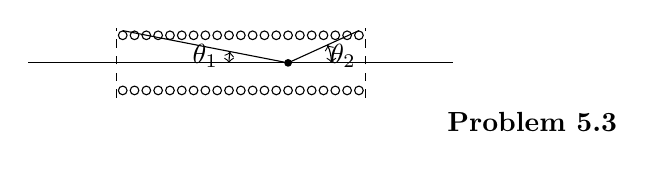
\begin{tikzpicture}[scale=1.0]
  % solenoid: two rows of coil cross-section circles
  \foreach \i in {0,...,20}{
    \draw (\i*0.15,0.35) circle (0.055);
    \draw (\i*0.15,-0.35) circle (0.055);
  }
  % dashed end caps
  \draw[dashed] (-0.08,-0.44) -- (-0.08,0.44);
  \draw[dashed] (3.08,-0.44) -- (3.08,0.44);
  % axis
  \draw (-1.2,0) -- (4.2,0);
  % point P on the axis, right of center
  \fill (2.1,0) circle (1.4pt);
  % lines from ends of solenoid to P
  \draw (0,0.41) -- (2.1,0);
  \draw (3.0,0.41) -- (2.1,0);
  % theta angles: arcs between axis and slanted lines, centered at P
  \draw[<->] (1.35,0) arc (180:169:0.75);
  \node at (1.05,0.09) {$\theta_{1}$};
  \draw[<->] (2.65,0) arc (0:24.5:0.55);
  \node at (2.8,0.09) {$\theta_{2}$};
  \node[below right] at (4.0,-0.5) {\textbf{Problem 5.3}};
\end{tikzpicture}
\end{center}
\solution
First derive the axial field of one loop. Parameterize it by
\[
\mathbf x'=(a\cos\phi',a\sin\phi',z'),\qquad
d\mathbf l'=a(-\sin\phi',\cos\phi',0)d\phi'.
\]
Then
the axial component of $d\mathbf l'\times(\mathbf x-\mathbf x')$
at $(0,0,z)$ is $a^2d\phi'$. The transverse components integrate to zero,
so
\[
dB_z=\frac{\mu_0(NI\,dz')a^2}
{2[a^2+(z-z')^2]^{3/2}}.
\]
Choose the ends at $\pm L/2$ and integrate:
\[
\begin{split}
B_z(z)&=\frac{\mu_0NI}{2}\int_{-L/2}^{L/2}
\frac{a^2\,dz'}{[a^2+(z-z')^2]^{3/2}}\\
&=\frac{\mu_0NI}{2}
\left[\frac{z+L/2}{\sqrt{a^2+(z+L/2)^2}}
-\frac{z-L/2}{\sqrt{a^2+(z-L/2)^2}}\right].
\end{split}
\]
The antiderivative used here is
$u/\sqrt{a^2+u^2}$, whose derivative is $a^2/(a^2+u^2)^{3/2}$.
For a point between the ends,
\[
\cos\theta_1=\frac{z+L/2}{\sqrt{a^2+(z+L/2)^2}},\qquad
\cos\theta_2=\frac{L/2-z}{\sqrt{a^2+(L/2-z)^2}},
\]
which proves the stated result. The algebraic formula also applies
outside the solenoid, with the corresponding signed cosines.
The continuum limit replaces the discrete turns by a sheet of current
$NI$; a long solenoid gives $B_z\to\mu_0NI$ deep inside.


\Needspace{5\baselineskip}
\par\bigskip
\noindent\textbf{5.4}\quad A magnetic induction $\mathbf{B}$ in a current-free region in a uniform medium is cylindrically symmetric with components $B_{z}(\rho,z)$ and $B_{\rho}(\rho,z)$ and with a known $B_{z}(0,z)$ on the axis of symmetry. The magnitude of the axial field varies slowly in $z$.
\begin{enumerate}
\item[(a)] Show that near the axis the axial and radial components of magnetic induction are approximately
\begin{align*}
B_{z}(\rho,z)&\simeq B_{z}(0,z)-\left(\frac{\rho^{2}}{4}\right)\!\left[\frac{\partial^{2}B_{z}(0,z)}{\partial z^{2}}\right]+\cdots\\
B_{\rho}(\rho,z)&\simeq-\left(\frac{\rho}{2}\right)\!\left[\frac{\partial B_{z}(0,z)}{\partial z}\right]+\left(\frac{\rho^{3}}{16}\right)\!\left[\frac{\partial^{3}B_{z}(0,z)}{\partial z^{3}}\right]+\cdots
\end{align*}
\item[(b)] What are the magnitudes of the neglected terms, or equivalently what is the criterion defining ``near'' the axis?
\end{enumerate}
\solution
\textbf{(a)} Smooth axial symmetry requires expansions
\[
B_z(\rho,z)=\sum_{n=0}^\infty a_n(z)\rho^{2n},\qquad
B_\rho(\rho,z)=\sum_{n=0}^\infty b_n(z)\rho^{2n+1}.
\]
The divergence equation and the azimuthal curl equation are
\[
\rho^{-1}\partial_\rho(\rho B_\rho)+\partial_zB_z=0,\qquad
\partial_zB_\rho-\partial_\rho B_z=0.
\]
Equating powers of $\rho$ gives
\[
(2n+2)b_n+a_n'=0,\qquad b_n'=2(n+1)a_{n+1}.
\]
Combining these, $a_{n+1}=-a_n''/[4(n+1)^2]$.
Writing $f(z)=B_z(0,z)=a_0(z)$, repeated substitution yields
\[
a_n=\frac{(-1)^nf^{(2n)}}{2^{2n}(n!)^2},\qquad
b_n=\frac{(-1)^{n+1}f^{(2n+1)}}{2^{2n+1}n!(n+1)!}.
\]
In particular,
\[
\boxed{B_z=f-\frac{\rho^2}{4}f''+\frac{\rho^4}{64}f^{(4)}+\cdots,}
\qquad
\boxed{B_\rho=-\frac{\rho}{2}f'+\frac{\rho^3}{16}f'''
-\frac{\rho^5}{384}f^{(5)}+\cdots.}
\]
\textbf{(b)} The first omitted terms in the question are
$\rho^4f^{(4)}/64$ and $-\rho^5f^{(5)}/384$.
If derivatives have a common variation length $\ell$,
$|f^{(n)}|\sim |f|/\ell^n$, the expansion parameter is $\rho/\ell\ll1$.
More precisely, each omitted term must be small relative to the accuracy
required of the retained sum. Ratios to $f'$ or $f''$ alone are
inappropriate where those derivatives happen to vanish. The series is
local and its radius of convergence cannot extend through a current sheet
or another field singularity.


\Needspace{5\baselineskip}
\par\bigskip
\noindent\textbf{5.5}\quad\begin{enumerate}
\item[(a)] Use the results of Problems 5.4 and 5.3 to find the axial and radial components of magnetic induction in the \emph{central region} ($|z|\ll L/2$) of a long uniform solenoid of radius $a$ and ends at $z=\pm L/2$, including the value of $B_{z}$ just inside the coil ($\rho=a^{-}$).
\item[(b)] Use Amp\`ere's law to show that the longitudinal magnetic induction just outside the coil is approximately
\[
B_{z}(\rho=a^{+},z)\simeq-\left(\frac{2\mu_{0}NIa^{2}}{L^{2}}\right)\!\left(1+\frac{12z^{2}}{L^{2}}-\frac{9a^{2}}{L^{2}}+\cdots\right)
\]
For $L\gg a$, the field outside is negligible compared to inside. How does this axial component compare in size to the azimuthal component of Problem 5.2b?
\item[(c)] Show that at the end of the solenoid the magnetic induction near the axis has components
\[
B_{z}\simeq\frac{\mu_{0}NI}{2},\qquad B_{\rho}\simeq\pm\frac{\mu_{0}NI}{4}\left(\frac{\rho}{a}\right)
\]
\end{enumerate}
\solution
Put $\ell=L/2$ and $B_s=\mu_0NI$. We consider $a,\rho,|z|\ll\ell$.
The exact on-axis result of 5.3 is
\[
\frac{f(z)}{B_s}
=\frac12\left[\frac{\ell+z}{\sqrt{a^2+(\ell+z)^2}}
+\frac{\ell-z}{\sqrt{a^2+(\ell-z)^2}}\right].
\]
Use $(1+x)^{-1/2}=1-x/2+3x^2/8+\cdots$ and then expand in $z/\ell$:
\[
\frac f{B_s}
=1-\frac{a^2}{2\ell^2}-\frac{3a^2z^2}{2\ell^4}
+\frac{3a^4}{8\ell^4}
+O\left(\frac{a^2z^4+a^4z^2+a^6}{\ell^6}\right).
\]
\textbf{(a)} Differentiating this axis function and using 5.4 gives
\[
\boxed{\frac{B_z}{B_s}
=1-\frac{a^2}{2\ell^2}
-\frac{3a^2z^2}{2\ell^4}
+\frac{3a^4}{8\ell^4}
+\frac{3a^2\rho^2}{4\ell^4}+\cdots,\qquad
\frac{B_\rho}{B_s}=\frac{3a^2\rho z}{2\ell^4}+\cdots.}
\]
For example, the next terms in $B_\rho/B_s$ are
$5a^2\rho z^3/\ell^6-15a^4\rho z/(4\ell^6)
-15a^2\rho^3z/(4\ell^6)$.
At the inner wall,
\[
B_z(a^-,z)=B_s\left[1-\frac{2a^2}{L^2}
-\frac{24a^2z^2}{L^4}+\frac{18a^4}{L^4}+\cdots\right].
\]
\textbf{(b)} A narrow rectangular Ampere loop straddling the winding
gives $H_z(a^-)-H_z(a^+)=NI$. Subtracting $B_s$ from the preceding
expression therefore gives
\[
\boxed{B_z(a^+,z)=-\frac{2\mu_0NIa^2}{L^2}
\left[1+\frac{12z^2}{L^2}-\frac{9a^2}{L^2}+\cdots\right].}
\]
It is an axial return field. For an actual helical winding,
$B_\phi(a^+)=\mu_0I/(2\pi a)$, so near the center
\[
\frac{|B_z(a^+)|}{|B_\phi(a^+)|}\simeq
\frac{4\pi Na^3}{L^2}.
\]
Thus either exterior component can dominate, depending on $N,a,L$;
both can be small compared with the main interior field.

\textbf{(c)} At the upper end $z=\ell$,
\[
f(\ell)=\frac{B_s}{2}\frac{L}{\sqrt{L^2+a^2}}
\simeq\frac{B_s}{2},\qquad
f'(\ell)=\frac{B_s}{2}
\left[\frac{a^2}{(L^2+a^2)^{3/2}}-\frac1a\right]
\simeq-\frac{B_s}{2a}.
\]
For $\rho\ll a$ and $L\gg a$, 5.4 then gives
$B_\rho\simeq B_s\rho/(4a)$. At the lower end the derivative changes
sign. Consequently
\[
\boxed{B_z\simeq B_s/2,\qquad
B_\rho\simeq\pm B_s\rho/(4a)}
\]
at the upper/lower ends, respectively.


\Needspace{5\baselineskip}
\par\bigskip
\noindent\textbf{5.6}\quad A cylindrical conductor of radius $a$ has a hole of radius $b$ bored parallel to, and centered a distance $d$ from, the cylinder axis ($d+b<a$). The current density is uniform throughout the remaining metal of the cylinder and is parallel to the axis. Use Amp\`ere's law and principle of linear superposition to find the magnitude and the direction of the magnetic-flux density in the hole.
\solution
Let the axis of the original cylinder be the origin of transverse
coordinates, and let the hole center have displacement $\mathbf d$.
Take $\mathbf J=J\widehat{\mathbf z}$ in the remaining metal.
For a uniformly filled cylinder, an Amperian circle gives
$2\pi\rho B_\phi=\mu_0J\pi\rho^2$, or
\[
\mathbf B_{\rm full}(\boldsymbol\rho)
=\frac{\mu_0}{2}\mathbf J\times\boldsymbol\rho.
\]
Represent the hole by superposing a cylinder with density $-\mathbf J$
and local coordinate $\boldsymbol\rho-\mathbf d$. Every point in the
hole is inside both cylinders, so
\[
\boxed{\mathbf B_{\rm hole}
=\frac{\mu_0}{2}\left[\mathbf J\times\boldsymbol\rho
-\mathbf J\times(\boldsymbol\rho-\mathbf d)\right]
=\frac{\mu_0}{2}\mathbf J\times\mathbf d.}
\]
The field is uniform, of magnitude $\mu_0Jd/2$, perpendicular both to
the current and to the displacement toward the hole. If the total
current is $I$, then $J=I/[\pi(a^2-b^2)]$. A centered hole gives zero
field, providing a symmetry check.


\Needspace{5\baselineskip}
\par\bigskip
\noindent\textbf{5.7}\quad A compact circular coil of radius $a$, carrying a current $I$ (perhaps $N$ turns, each with current $I/N$), lies in the $x$-$y$ plane with its center at the origin.
\begin{enumerate}
\item[(a)] By elementary means [Eq.~(5.4)] find the magnetic induction at any point on the $z$ axis.
\item[(b)] An identical coil with the same magnitude and sense of the current is located on the same axis, parallel to, and a distance $b$ above, the first coil. With the coordinate origin relocated at the point midway between the centers of the two coils, determine the magnetic induction on the axis near the origin as an expansion in powers of $z$, up to $z^{4}$ inclusive:
\[
B_{z}=\left(\frac{\mu_{0}Ia^{2}}{d^{3}}\right)\!\left[1+\frac{3(b^{2}-a^{2})z^{2}}{2d^{4}}+\frac{15(b^{4}-6b^{2}a^{2}+2a^{4})z^{4}}{16d^{8}}+\cdots\right]
\]
where $d^{2}=a^{2}+b^{2}/4$.
\item[(c)] Show that, off-axis near the origin, the axial and radial components, correct to second order in the coordinates, take the form
\[
B_{z}=\sigma_{0}+\sigma_{2}\left(z^{2}-\frac{\rho^{2}}{2}\right);\qquad B_{\rho}=-\sigma_{2}z\rho
\]
\item[(d)] For the two coils in part b show that the magnetic induction on the $z$ axis for large $|z|$ is given by the expansion in inverse odd powers of $|z|$ obtained from the small $z$ expansion of part b by the formal substitution, $d\to|z|$.
\item[(e)] If $b=a$, the two coils are known as a pair of Helmholtz coils. For this choice of geometry the second terms in the expansions of parts b and d are absent ($\sigma_{2}=0$ in part c). The field near the origin is then very uniform. What is the maximum permitted value of $|z|/a$ if the axial field is to be uniform to one part in $10^{4}$, one part in $10^{2}$?
\end{enumerate}
\solution
\textbf{(a)} The element calculation in 5.3 gives
\[
\boxed{B_z(0,z)=\frac{\mu_0Ia^2}{2(a^2+z^2)^{3/2}},\qquad
B_x=B_y=0.}
\]
Here $I$ is the total ampere-turns specified in the question.

\textbf{(b)} Put the centers at $z=\pm b/2$ and
$d^2=a^2+b^2/4$. The exact sum is
\[
B_z=\frac{\mu_0Ia^2}{2d^3}
\left[\left(1+\frac{z^2-bz}{d^2}\right)^{-3/2}
+\left(1+\frac{z^2+bz}{d^2}\right)^{-3/2}\right].
\]
The binomial coefficients needed are
$1,-3/2,15/8,-35/16,315/128$.
After averaging the two signs, the coefficients of $z^2$ and $z^4$ are
\[
-\frac3{2d^2}+\frac{15b^2}{8d^4}
=\frac{3(b^2-a^2)}{2d^4},
\]
\[
\frac{15}{8d^4}-\frac{105b^2}{16d^6}
+\frac{315b^4}{128d^8}
=\frac{15(b^4-6a^2b^2+2a^4)}{16d^8}.
\]
The odd powers cancel, proving the stated series.

\textbf{(c)} Write its first terms as $f(z)=\sigma_0+\sigma_2z^2+\cdots$,
where
\[
\sigma_0=\frac{\mu_0Ia^2}{d^3},\qquad
\sigma_2=\sigma_0\frac{3(b^2-a^2)}{2d^4}.
\]
Then $f'=2\sigma_2z+\cdots$ and $f''=2\sigma_2+\cdots$.
Substitution into 5.4 gives
\[
\boxed{B_z=\sigma_0+\sigma_2(z^2-\rho^2/2)+O(r^4),\qquad
B_\rho=-\sigma_2z\rho+O(r^4).}
\]
\textbf{(d)} For $|z|\gg d$, factor $|z|^3$ from the exact denominators:
\[
B_z=\frac{\mu_0Ia^2}{2|z|^3}
\sum_{\pm}\left(1\pm\frac b{|z|}+\frac{d^2}{z^2}\right)^{-3/2}.
\]
The same binomial calculation yields
\[
\boxed{B_z=\frac{\mu_0Ia^2}{|z|^3}
\left[1+\frac{3(b^2-a^2)}{2z^2}
+\frac{15(b^4-6a^2b^2+2a^4)}{16z^4}+\cdots\right].}
\]
This is the stated formal replacement $d\mapsto|z|$ in part (b),
including its prefactor. It does not replace $a$ or $b$.

\textbf{(e)} At $b=a$, $d^2=5a^2/4$ and
\[
\frac{B_z(z)}{B_z(0)}
=1-\frac{144}{125}(z/a)^4+O((z/a)^6).
\]
The fourth-order estimate for relative tolerance $\delta$ is
$|z|/a\le(125\delta/144)^{1/4}$, namely $0.09652$ for $10^{-4}$
and $0.30524$ for $10^{-2}$. To determine the actual edge of the
central uniform interval, solve with the exact field:
\[
\frac{(5/4)^{3/2}}2
\left\{[1+(u-1/2)^2]^{-3/2}+[1+(u+1/2)^2]^{-3/2}\right\}
=1-\delta,\qquad u=|z|/a.
\]
The exact central-interval limits are
$\boxed{|z|/a\le0.0967727}$ and $\boxed{|z|/a\le0.3137460}$,
respectively. Substitution into the exact expression gives field ratios
$0.9999$ and $0.9900$.


\Needspace{5\baselineskip}
\par\bigskip
\noindent\textbf{5.8}\quad A localized cylindrically symmetric current distribution is such that the current flows only in the azimuthal direction; the current density is a function only of $r$ and $\theta$ (or $\rho$ and $z$): $\mathbf{J}=\hat{\boldsymbol{\phi}}J(r,\theta)$. The distribution is ``hollow'' in the sense that there is a current-free region near the origin, as well as outside.
\begin{enumerate}
\item[(a)] Show that the magnetic field can be derived from the azimuthal component of the vector potential, with a multipole expansion
\[
A_{\phi}(r,\theta)=-\frac{\mu_{0}}{4\pi}\sum_{L}m_{L}r^{L}P_{L}^{1}(\cos\theta)
\]
in the interior and
\[
A_{\phi}(r,\theta)=-\frac{\mu_{0}}{4\pi}\sum_{L}\mu_{L}r^{-L-1}P_{L}^{1}(\cos\theta)
\]
outside the current distribution.
\item[(b)] Show that the internal and external multipole moments are
\[
m_{L}=-\frac{1}{L(L+1)}\int d^{3}x\;r^{-L-1}P_{L}^{1}(\cos\theta)\,J(r,\theta)
\]
and
\[
\mu_{L}=-\frac{1}{L(L+1)}\int d^{3}x\;r^{L}P_{L}^{1}(\cos\theta)\,J(r,\theta)
\]
\end{enumerate}
\solution
\textbf{(a)} Choose the observation azimuth to be zero. Reflection in the
$x$--$z$ plane cancels the radial part of
$\mathbf A=(\mu_0/4\pi)\int\mathbf J(\mathbf x')/|\mathbf x-\mathbf x'|\,d^3x'$.
There is no $z$ component, and
\[
A_\phi=\frac{\mu_0}{4\pi}\int
\frac{J(r',\theta')\cos\phi'}{|\mathbf x-\mathbf x'|}\,d^3x'.
\]
Expand the Coulomb kernel as
$\sum_{L\ge0}r_<^Lr_>^{-L-1}P_L(\cos\gamma)$.
The addition theorem in real azimuthal form is
\[
P_L(\cos\gamma)=P_L(\cos\theta)P_L(\cos\theta')
+2\sum_{m=1}^L\frac{(L-m)!}{(L+m)!}
P_L^m(\cos\theta)P_L^m(\cos\theta')\cos(m\phi').
\]
Multiplication by $\cos\phi'$ and integration over $0\le\phi'<2\pi$
kills every term except $m=1$, whose cosine integral is $\pi$.
Thus
\[
A_\phi=\frac{\mu_0}{4\pi}\sum_{L=1}^\infty
\frac{P_L^1(\cos\theta)}{L(L+1)}
\int d^3x'\,\frac{r_<^L}{r_>^{L+1}}
P_L^1(\cos\theta')J(r',\theta').
\]
\textbf{(b)} In a source-free ball containing the origin, $r<r'$ for
all source points, so factor out $r^L$. In the exterior of a sphere
containing all currents, $r>r'$ and one factors out $r^{-L-1}$.
Define
\[
\boxed{m_L=-\frac1{L(L+1)}\int r'^{-L-1}P_L^1(\cos\theta')J\,d^3x',
\qquad
\mu_L=-\frac1{L(L+1)}\int r'^LP_L^1(\cos\theta')J\,d^3x'.}
\]
Then
\[
\boxed{A_{\phi,\rm in}=-\frac{\mu_0}{4\pi}\sum_{L\ge1}m_Lr^LP_L^1,
\qquad
A_{\phi,\rm out}=-\frac{\mu_0}{4\pi}\sum_{L\ge1}\mu_Lr^{-L-1}P_L^1.}
\]
The moments use the Condon--Shortley convention
$P_L^1(\cos\theta)=\partial_\theta P_L(\cos\theta)$.
Finally,
$B_r=(r\sin\theta)^{-1}\partial_\theta(\sin\theta A_\phi)$ and
$B_\theta=-r^{-1}\partial_r(rA_\phi)$, with $B_\phi=0$.
These convergence domains are spherical source-free regions; an
arbitrary point merely outside the current support need not belong to
the convergence domain of either expansion.


\Needspace{5\baselineskip}
\par\bigskip
\noindent\textbf{5.9}\quad The two circular coils of radius $a$ and separation $b$ of Problem 5.7 can be described in cylindrical coordinates by the current density
\[
\mathbf{J}=\hat{\boldsymbol{\phi}}I\delta(\rho-a)[\delta(z-b/2)+\delta(z+b/2)]
\]
\begin{enumerate}
\item[(a)] Using the formalism of Problem 5.8, calculate the internal and external multipole moments for $L=1,\ldots,5$.
\item[(b)] Using the internal multipole expansion of Problem 5.8, write down explicitly an expression for $B_{z}$ on the $z$ axis and relate it to the answer of Problem 5.7b.
\end{enumerate}
\solution
\textbf{(a)} Let $d=\sqrt{a^2+b^2/4}$ and $c=b/(2d)$.
At the two source rings, $r'=d$ and $\cos\theta'=\pm c$.
The cylindrical volume element supplies
$\int J\,d^3x'=2\pi aI$ for each ring.
Because $P_L^1(-c)=(-1)^{L+1}P_L^1(c)$, even $L$ vanish and odd $L$ give
\[
m_L=-\frac{4\pi aI}{L(L+1)d^{L+1}}P_L^1(c),\qquad
\mu_L=d^{2L+1}m_L.
\]
Use
\[
P_1^1(c)=-\sqrt{1-c^2},\quad
P_3^1(c)=-\tfrac32(5c^2-1)\sqrt{1-c^2},\quad
P_5^1(c)=-\tfrac{15}{8}(21c^4-14c^2+1)\sqrt{1-c^2},
\]
with $\sqrt{1-c^2}=a/d$. The explicit moments are
\[
\begin{array}{c|c|c}
L&m_L&\mu_L\\\hline
1&2\pi Ia^2/d^3&2\pi Ia^2\\[2pt]
2&0&0\\[2pt]
3&\pi Ia^2(b^2-a^2)/(2d^7)&\pi Ia^2(b^2-a^2)/2\\[2pt]
4&0&0\\[2pt]
5&\pi Ia^2(b^4-6a^2b^2+2a^4)/(8d^{11})
&\pi Ia^2(b^4-6a^2b^2+2a^4)/8
\end{array}
\]
\textbf{(b)} The identity $\partial_\theta(\sin\theta P_L^1)
=-L(L+1)\sin\theta P_L$ gives
\[
B_{r,\rm in}=\frac{\mu_0}{4\pi}
\sum_{L\ge1}L(L+1)m_Lr^{L-1}P_L(\cos\theta).
\]
On the positive $z$ axis $P_L(1)=1$ and $B_z=B_r$, hence
\[
B_z(0,z)=\frac{\mu_0}{4\pi}
[2m_1+12m_3z^2+30m_5z^4+\cdots].
\]
Inserting the table reproduces every coefficient in 5.7(b).
Reflection symmetry extends this even polynomial to negative $z$.


\Needspace{5\baselineskip}
\par\bigskip
\noindent\textbf{5.10}\quad A circular current loop of radius $a$ carrying a current $I$ lies in the $x$-$y$ plane with its center at the origin.
\begin{enumerate}
\item[(a)] Show that the only nonvanishing component of the vector potential is
\[
A_{\phi}(\rho,z)=\frac{\mu_{0}Ia}{\pi}\int_{0}^{\infty}dk\,\cos kz\,I_{1}(k\rho_{<})K_{1}(k\rho_{>})
\]
where $\rho_{<}$ ($\rho_{>}$) is the smaller (larger) of $a$ and $\rho$.
\item[(b)] Show that an alternative expression for $A_{\phi}$ is
\[
A_{\phi}(\rho,z)=\frac{\mu_{0}Ia}{2}\int_{0}^{\infty}dk\;e^{-k|z|}J_{1}(ka)J_{1}(k\rho)
\]
\item[(c)] Write down integral expressions for the components of magnetic induction, using the expressions of parts a and b. Evaluate explicitly the components of $\mathbf{B}$ on the $z$ axis by performing the necessary integrations.
\end{enumerate}
\solution
The scalar cylindrical Green expansions needed here follow by
separating the Fourier variable along $z$, or by separating radial
Bessel modes:
\[
\begin{split}
\frac1{|\mathbf x-\mathbf x'|}
&=\frac2\pi\sum_{m=-\infty}^{\infty}e^{im(\phi-\phi')}
\int_0^\infty \cos[k(z-z')]I_m(k\rho_<)K_m(k\rho_>)\,dk,\\
\frac1{|\mathbf x-\mathbf x'|}
&=\sum_{m=-\infty}^{\infty}e^{im(\phi-\phi')}
\int_0^\infty e^{-k|z-z'|}J_m(k\rho)J_m(k\rho')\,dk.
\end{split}
\]
For completeness, the first normalization follows from
$\int_0^\infty\cos(kz)K_0(ks)\,dk=\pi/[2\sqrt{s^2+z^2}]$ and
the cylindrical addition theorem for $K_0$.
The second follows from
$\int_0^\infty e^{-k|z|}J_0(ks)\,dk=1/\sqrt{s^2+z^2}$
and the addition theorem for $J_0$.

\textbf{(a),(b)} The current loop has $d\mathbf l'=a\widehat{\boldsymbol\phi}'d\phi'$.
Projecting onto the observation $\widehat{\boldsymbol\phi}$ supplies
$\cos(\phi-\phi')$. Its angular integral is $\pi$ for each of $m=\pm1$
and zero for all other $m$. Consequently the first kernel gives
\[
\boxed{A_\phi=\frac{\mu_0Ia}{\pi}\int_0^\infty
\cos(kz)I_1(k\rho_<)K_1(k\rho_>)\,dk,}
\]
and the second gives
\[
\boxed{A_\phi=\frac{\mu_0Ia}{2}\int_0^\infty
e^{-k|z|}J_1(ka)J_1(k\rho)\,dk.}
\]
All other components vanish by the same reflection symmetry as in 5.8.

\textbf{(c)} The curl equations are
$B_\rho=-\partial_zA_\phi$ and
$B_z=\rho^{-1}\partial_\rho(\rho A_\phi)$.
Using $(xI_1)'=xI_0$, $(xK_1)'=-xK_0$, and $(xJ_1)'=xJ_0$, one obtains
\[
B_\rho=\frac{\mu_0Ia}{\pi}\int_0^\infty
k\sin(kz)I_1(k\rho_<)K_1(k\rho_>)\,dk,
\]
\[
B_z=\frac{\mu_0Ia}{\pi}\int_0^\infty k\cos(kz)
\begin{cases}
I_0(k\rho)K_1(ka),&\rho<a,\\
-I_1(ka)K_0(k\rho),&\rho>a
\end{cases}dk,
\]
or, for $z\ne0$,
\[
\boxed{\begin{aligned}
B_\rho&=\frac{\mu_0Ia}{2}\operatorname{sgn}(z)
\int_0^\infty k e^{-k|z|}J_1(ka)J_1(k\rho)\,dk,\\
B_z&=\frac{\mu_0Ia}{2}\int_0^\infty
k e^{-k|z|}J_1(ka)J_0(k\rho)\,dk.
\end{aligned}}
\]
At $z=0$ off the wire, take the limiting fields; symmetry gives
$B_\rho=0$. On the axis $J_1(0)=0$ and $J_0(0)=1$.
Differentiate the elementary Laplace integral
$\int_0^\infty e^{-sk}J_0(ak)\,dk=(s^2+a^2)^{-1/2}$ with respect to $a$:
\[
\int_0^\infty k e^{-sk}J_1(ak)\,dk=\frac{a}{(s^2+a^2)^{3/2}}.
\]
This gives
$\boxed{B_\rho(0,z)=0,\ B_z(0,z)=\mu_0Ia^2/[2(a^2+z^2)^{3/2}]}$.
The modified-Bessel representation independently gives the same result:
differentiate
$\int_0^\infty\cos(kz)K_0(ka)\,dk=\pi/[2\sqrt{a^2+z^2}]$
with respect to $a$, producing the required integral of $kK_1(ka)$.


\Needspace{5\baselineskip}
\par\bigskip
\noindent\textbf{5.11}\quad A circular loop of wire carrying a current $I$ is located with its center at the origin of coordinates and the normal to its plane having spherical angles $\theta_{0}$, $\phi_{0}$. There is an applied magnetic field, $B_{x}=B_{0}(1+\beta y)$ and $B_{y}=B_{0}(1+\beta x)$.
\begin{enumerate}
\item[(a)] Calculate the force acting on the loop without making any approximations. Compare your result with the approximate result (5.69). Comment.
\item[(b)] Calculate the torque in lowest order. Can you deduce anything about the higher order contributions? Do they vanish for the circular loop? What about for other shapes?
\end{enumerate}
\solution
Let the radius be $a$, the area be $S=\pi a^2$, and
\[
\mathbf m=IS(\sin\theta_0\cos\phi_0,\sin\theta_0\sin\phi_0,\cos\theta_0).
\]
\textbf{(a)} Starting with
$\mathbf F=I\oint d\mathbf l\times\mathbf B$ and writing
$B_k=B_{k0}+G_{kj}x_j$, the constant term vanishes.
Stokes's theorem gives
$\oint x_j\,dx_i=\epsilon_{jil}S n_l$.
In indices, the remaining term is
\[
F_i=I\epsilon_{ijk}G_{k\ell}\oint x_\ell\,dx_j
=\epsilon_{ijk}\epsilon_{\ell jn}G_{k\ell}m_n
=m_kG_{ki}-m_iG_{kk}.
\]
Here $\epsilon_{ijk}\epsilon_{\ell jn}=\delta_{i\ell}\delta_{kn}
-\delta_{in}\delta_{k\ell}$ and $G_{kk}=\nabla\cdot\mathbf B=0$.
Therefore $F_i=m_j\partial_iB_j$.
Here $\partial_yB_x=\partial_xB_y=\beta B_0$, and thus
\[
\boxed{\mathbf F=\beta B_0(m_y,m_x,0)
=\beta B_0I\pi a^2\sin\theta_0
(\sin\phi_0,\cos\phi_0,0).}
\]
This is exactly $\nabla(\mathbf m\cdot\mathbf B)$, with no small-loop
approximation: a linear applied field has no derivatives that could
couple to higher force multipoles.

\textbf{(b)} To dipole order,
\[
\boxed{\mathbf N=\mathbf m\times\mathbf B(0)
=B_0(-m_z,m_z,m_x-m_y).}
\]
One can also see why this is exact for the centered circle. The torque
integrand is $\mathbf x\times[I\,d\mathbf l\times\mathbf B]$.
Its correction from the linear part of $\mathbf B$ is odd under
$(\mathbf x,d\mathbf l)\mapsto(-\mathbf x,-d\mathbf l)$, so opposite
points cancel. Terms beyond this correction are absent because the field
is linear.

For a general planar loop with area centroid
$\overline{\mathbf x}=S^{-1}\int_S\mathbf x\,da$, an explicit surface
form of the torque is
\[
\mathbf N=I\int_S\left[\mathbf n\times\mathbf B(\mathbf x)
+\mathbf x\times\nabla(\mathbf n\cdot\mathbf B)\right]da.
\]
This follows by dividing the spanning surface into small loops; all
interior edges cancel, leaving the original boundary loop.
For the present linear field it becomes
\[
\mathbf N=\mathbf m\times[\mathbf B(0)+G\overline{\mathbf x}]
+\overline{\mathbf x}\times(G^T\mathbf m).
\]
Thus a general shape can have a correction about a specified origin.
It vanishes for every planar shape when the origin is its area centroid,
not only for circles or shapes with inversion symmetry.


\Needspace{5\baselineskip}
\par\bigskip
\noindent\textbf{5.12}\quad Two concentric circular loops of radii $a$, $b$ and currents $I$, $I'$, respectively ($b<a$), have an angle $\alpha$ between their planes. Show that the torque on one of the loops is about the line of intersection of the two planes containing the loops and has the \erratum{signed component in the direction of increasing $\alpha$}
\[
\erratum{N_\alpha}=\frac{\mu_{0}\pi II'b^{2}}{2a}\sum_{n=0}^{\infty}\frac{(n+1)}{(2n+1)}\left[\frac{\Gamma(n+\frac{3}{2})}{\Gamma(n+2)\Gamma(\frac{3}{2})}\right]^{2}\!\left(\frac{b}{a}\right)^{2n}\!P_{2n+1}^{1}(\cos\alpha)
\]
where $P_{l}^{1}(\cos\alpha)$ is an associated Legendre polynomial. Determine the sense of the torque for $\alpha$ an acute angle and the currents in the same (opposite) directions.
\solution
Take the larger loop's normal along $z$ and let $\alpha$ be the angle
through which the smaller normal is rotated about the line of intersection.
We use $P_l^1(\cos\alpha)=dP_l(\cos\alpha)/d\alpha$.
For the single larger loop, the interior moment from 5.8 is
\[
m_l=-\frac{2\pi I}{l(l+1)a^l}P_l^1(0),\qquad l=1,3,5,\ldots.
\]
Its scalar potential for $\mathbf H$ is
\[
\Phi_H=-\frac1{4\pi}\sum_l(l+1)m_lr^lP_l(\cos\theta),
\]
as direct radial differentiation verifies against the curl of $A_\phi$.

Introduce coordinates with $z'$ normal to the smaller loop.
Azimuthal averaging about that axis, using the addition theorem, replaces
$P_l(\cos\theta)$ by $P_l(\cos\alpha)P_l(\cos\theta')$.
On its spanning disk $z'=0$,
\[
\left.\partial_{z'}[r^lP_l(z'/r)]\right|_{z'=0}
=r^{l-1}P_l'(0)=-r^{l-1}P_l^1(0).
\]
Integrating $B_{z'}=-\mu_0\partial_{z'}\Phi_H$ over the disk gives its flux:
\[
\begin{split}
F&=-\frac{\mu_0}{4\pi}\sum_l(l+1)m_lP_l^1(0)P_l(\cos\alpha)
\int_0^b2\pi r^l\,dr\\
&=-\frac{\mu_0}{2}\sum_lm_lP_l^1(0)b^{l+1}P_l(\cos\alpha).
\end{split}
\]
Thus
\[
M(\alpha)=F/I=\mu_0\pi\sum_{l\ {\rm odd}}
\frac{[P_l^1(0)]^2}{l(l+1)}
\frac{b^{l+1}}{a^l}P_l(\cos\alpha).
\]
At fixed currents the torque component that increases $\alpha$ is
$N_\alpha=II'\,dM/d\alpha$. Put $l=2n+1$ and use
\[
P_{2n+1}^1(0)=(-1)^{n+1}\frac{(2n+1)!!}{(2n)!!}
=(-1)^{n+1}(n+1)
\frac{\Gamma(n+3/2)}{\Gamma(n+2)\Gamma(3/2)}.
\]
Then
\[
\boxed{N_\alpha=\frac{\mu_0\pi II'b^2}{2a}
\sum_{n=0}^\infty\frac{n+1}{2n+1}
\left[\frac{\Gamma(n+3/2)}{\Gamma(n+2)\Gamma(3/2)}\right]^2
\left(\frac ba\right)^{2n}P_{2n+1}^1(\cos\alpha).}
\]
The mechanical interaction potential is $-II'M$, which fixes this sign.
The displayed expression is a signed component, not an always-positive
magnitude; the magnitude is $|N_\alpha|$.

For $0<\alpha<\pi/2$, like-directed currents tend to decrease $\alpha$,
and opposite currents tend to increase it. To establish the sign beyond
the dipole limit, put $c=\cos\alpha>0$ and parameterize the smaller ring.
Its cylindrical radius satisfies
$\rho^2=b^2(\cos^2\varphi+c^2\sin^2\varphi)$, and
$\mathbf A\cdot d\mathbf l=b^2c(A_\phi/\rho)d\varphi$.
On the sphere $r=b<a$, the Biot--Savart expression for $A_\phi/\rho$
has a convergent expansion in nonnegative powers of $\rho^2$ with
positive coefficients: expand
$[a^2+b^2-2a\rho\cos\varphi']^{-1/2}$ and integrate its product with
$\cos\varphi'$. Only positive even cosine integrals survive.
Hence $M(c)=c$ times a positive, increasing function of $c^2$,
so $dM/d\alpha=-\sin\alpha\,dM/dc<0$.
Rotational symmetry leaves only a torque about the line of intersection.


\Needspace{5\baselineskip}
\par\bigskip
\noindent\textbf{5.13}\quad A sphere of radius $a$ carries a uniform surface-charge distribution $\sigma$. The sphere is rotated about a diameter with constant angular velocity $\omega$. Find the vector potential and magnetic-flux density both inside and outside the sphere.
\solution
Take $\boldsymbol\omega=\omega\widehat{\mathbf z}$. The moving surface
charge is the surface current
$\mathbf K=\sigma(\boldsymbol\omega\times\mathbf r)
=\sigma\omega a\sin\theta\,\widehat{\boldsymbol\phi}$.
It has only the $l=1$ angular dependence, so write
\[
A_\phi=\begin{cases}Cr\sin\theta,&r<a,\\D r^{-2}\sin\theta,&r>a.\end{cases}
\]
Continuity of $A_\phi$ gives $D=Ca^3$. Taking its curl gives
\[
\mathbf B_{\rm in}=2C(\cos\theta\,\widehat{\mathbf r}
-\sin\theta\,\widehat{\boldsymbol\theta}),\quad
\mathbf B_{\rm out}=\frac D{r^3}
(2\cos\theta\,\widehat{\mathbf r}+\sin\theta\,\widehat{\boldsymbol\theta}).
\]
The normal component is continuous, while the sheet-current condition is
$B_{\theta,\rm out}-B_{\theta,\rm in}=\mu_0K_\phi$.
Thus $3C\sin\theta=\mu_0\sigma\omega a\sin\theta$, giving
\[
\boxed{A_\phi=\frac{\mu_0\sigma\omega a}{3}
\begin{cases}r\sin\theta,&r<a,\\a^3r^{-2}\sin\theta,&r>a,\end{cases}}
\]
\[
\boxed{\mathbf B_{\rm in}=\frac{2\mu_0\sigma\omega a}{3}\widehat{\mathbf z},
\qquad
\mathbf B_{\rm out}=\frac{\mu_0\sigma\omega a^4}{3r^3}
(2\cos\theta\,\widehat{\mathbf r}+\sin\theta\,\widehat{\boldsymbol\theta}).}
\]
The external moment is
$\mathbf m=(4\pi\sigma\omega a^4/3)\widehat{\mathbf z}
=(Q\omega a^2/3)\widehat{\mathbf z}$.
Independently, $\mathbf m=\frac12\int\mathbf r\times\mathbf K\,da$
gives $m_z=(\sigma\omega a^2/2)\int\sin^2\theta\,da
=4\pi\sigma\omega a^4/3$.


\Needspace{5\baselineskip}
\par\bigskip
\noindent\textbf{5.14}\quad A long, hollow, right circular cylinder of inner (outer) radius $a$ ($b$), and of relative permeability $\mu_{r}$, is placed in a region of initially uniform magnetic-flux density $\mathbf{B}_{0}$ at right angles to the field. Find the flux density at all points in space, and sketch the logarithm of the ratio of the magnitudes of $\mathbf{B}$ on the cylinder axis to $\mathbf{B}_{0}$ as a function of $\log_{10}\mu_{r}$ for $a^{2}/b^{2}=0.5$, 0.1. Neglect end effects.
\solution
Let $\kappa=\mu_r>0$, $\eta=a^2/b^2$, and put the original field along
$x$. The magnetic scalar potential for $\mathbf H$ obeys the same
boundary equations as the dielectric-shell potential of Problem 4.8:
$H_\phi$ and $\mu H_\rho$ are continuous. Define
\[
\Delta=(\kappa+1)^2-(\kappa-1)^2\eta,\qquad
A=\frac{4\kappa}{\Delta},\quad B=\frac{2(\kappa+1)}{\Delta},\quad
C=\frac{2(\kappa-1)a^2}{\Delta},\quad
D=\frac{(\kappa^2-1)(b^2-a^2)}{\Delta}.
\]
In detail, the trial potential
$\Phi_H=-(B_0/\mu_0)\cos\phi\{A\rho,\ B\rho+C/\rho,\ \rho-D/\rho\}$
gives the four interface equations
\[
A=B+C/a^2,\quad A=\kappa(B-C/a^2),\quad
B+C/b^2=1-D/b^2,\quad \kappa(B-C/b^2)=1+D/b^2.
\]
The first pair gives
$C=a^2(\kappa-1)B/(\kappa+1)$ and
$A=2\kappa B/(\kappa+1)$.
Adding the last two equations eliminates $D$:
\[
(\kappa+1)B-(\kappa-1)C/b^2=2,\qquad
\frac{(\kappa+1)^2-(\kappa-1)^2\eta}{\kappa+1}B=2.
\]
Thus $B=2(\kappa+1)/\Delta$, which gives $A,C$ above.
Finally
\[
\frac D{b^2}=1-B-\frac C{b^2}
=\frac{\Delta-2(\kappa+1)-2(\kappa-1)\eta}{\Delta}
=\frac{(\kappa^2-1)(1-\eta)}{\Delta}.
\]
The requested induction components are
\[
\boxed{\frac{B_\rho}{B_0}=\cos\phi
\begin{cases}A,&\rho<a,\\\kappa(B-C/\rho^2),&a<\rho<b,\\
1+D/\rho^2,&\rho>b,\end{cases}}
\]
\[
\boxed{\frac{B_\phi}{B_0}=-\sin\phi
\begin{cases}A,&\rho<a,\\\kappa(B+C/\rho^2),&a<\rho<b,\\
1-D/\rho^2,&\rho>b,\end{cases}\qquad B_z=0.}
\]
In particular the core field is uniform, with
\[
F=\frac{|\mathbf B_{\rm core}|}{B_0}
=\frac{4\kappa}{(1-\eta)(\kappa^2+1)+2(1+\eta)\kappa}.
\]
The logarithmic curves below use $x=\log_{10}\kappa$ and $y=\log_{10}F$.
They are symmetric under $x\mapsto-x$, since $F(\kappa)=F(1/\kappa)$.
Both reach $F=1$ at $\kappa=1$; at large $\kappa$,
$F\sim4/[(1-\eta)\kappa]$, while at small $\kappa$,
$F\sim4\kappa/(1-\eta)$.
\begin{center}
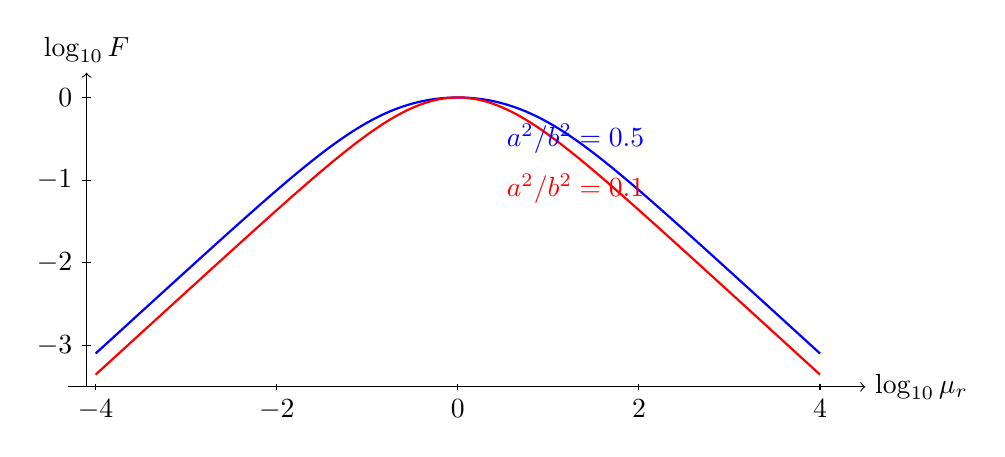
\begin{tikzpicture}[x=1.15cm,y=1.05cm]
\draw[->] (-4.3,-3.5)--(4.5,-3.5) node[right] {$\log_{10}\mu_r$};
\draw[->] (-4.1,-3.5)--(-4.1,.3) node[above] {$\log_{10}F$};
\draw[blue,thick] plot coordinates {(-4.0000000,-3.0971705) (-3.9500000,-3.0472023) (-3.9000000,-2.9972379) (-3.8500000,-2.9472779) (-3.8000000,-2.8973228) (-3.7500000,-2.8473732) (-3.7000000,-2.7974296) (-3.6500000,-2.7474930) (-3.6000000,-2.6975641) (-3.5500000,-2.6476438) (-3.5000000,-2.5977333) (-3.4500000,-2.5478336) (-3.4000000,-2.4979462) (-3.3500000,-2.4480725) (-3.3000000,-2.3982141) (-3.2500000,-2.3483730) (-3.2000000,-2.2985512) (-3.1500000,-2.2487511) (-3.1000000,-2.1989752) (-3.0500000,-2.1492266) (-3.0000000,-2.0995084) (-2.9500000,-2.0498245) (-2.9000000,-2.0001788) (-2.8500000,-1.9505761) (-2.8000000,-1.9010214) (-2.7500000,-1.8515206) (-2.7000000,-1.8020800) (-2.6500000,-1.7527069) (-2.6000000,-1.7034093) (-2.5500000,-1.6541961) (-2.5000000,-1.6050772) (-2.4500000,-1.5560639) (-2.4000000,-1.5071685) (-2.3500000,-1.4584047) (-2.3000000,-1.4097879) (-2.2500000,-1.3613348) (-2.2000000,-1.3130644) (-2.1500000,-1.2649973) (-2.1000000,-1.2171564) (-2.0500000,-1.1695670) (-2.0000000,-1.1222568) (-1.9500000,-1.0752563) (-1.9000000,-1.0285988) (-1.8500000,-0.9823204) (-1.8000000,-0.9364609) (-1.7500000,-0.8910627) (-1.7000000,-0.8461722) (-1.6500000,-0.8018387) (-1.6000000,-0.7581152) (-1.5500000,-0.7150578) (-1.5000000,-0.6727257) (-1.4500000,-0.6311813) (-1.4000000,-0.5904890) (-1.3500000,-0.5507156) (-1.3000000,-0.5119292) (-1.2500000,-0.4741986) (-1.2000000,-0.4375926) (-1.1500000,-0.4021790) (-1.1000000,-0.3680238) (-1.0500000,-0.3351898) (-1.0000000,-0.3037359) (-0.9500000,-0.2737161) (-0.9000000,-0.2451786) (-0.8500000,-0.2181648) (-0.8000000,-0.1927090) (-0.7500000,-0.1688377) (-0.7000000,-0.1465698) (-0.6500000,-0.1259165) (-0.6000000,-0.1068816) (-0.5500000,-0.0894623) (-0.5000000,-0.0736499) (-0.4500000,-0.0594307) (-0.4000000,-0.0467874) (-0.3500000,-0.0357001) (-0.3000000,-0.0261475) (-0.2500000,-0.0181084) (-0.2000000,-0.0115625) (-0.1500000,-0.0064919) (-0.1000000,-0.0028814) (-0.0500000,-0.0007198) (0.0000000,0.0000000) (0.0500000,-0.0007198) (0.1000000,-0.0028814) (0.1500000,-0.0064919) (0.2000000,-0.0115625) (0.2500000,-0.0181084) (0.3000000,-0.0261475) (0.3500000,-0.0357001) (0.4000000,-0.0467874) (0.4500000,-0.0594307) (0.5000000,-0.0736499) (0.5500000,-0.0894623) (0.6000000,-0.1068816) (0.6500000,-0.1259165) (0.7000000,-0.1465698) (0.7500000,-0.1688377) (0.8000000,-0.1927090) (0.8500000,-0.2181648) (0.9000000,-0.2451786) (0.9500000,-0.2737161) (1.0000000,-0.3037359) (1.0500000,-0.3351898) (1.1000000,-0.3680238) (1.1500000,-0.4021790) (1.2000000,-0.4375926) (1.2500000,-0.4741986) (1.3000000,-0.5119292) (1.3500000,-0.5507156) (1.4000000,-0.5904890) (1.4500000,-0.6311813) (1.5000000,-0.6727257) (1.5500000,-0.7150578) (1.6000000,-0.7581152) (1.6500000,-0.8018387) (1.7000000,-0.8461722) (1.7500000,-0.8910627) (1.8000000,-0.9364609) (1.8500000,-0.9823204) (1.9000000,-1.0285988) (1.9500000,-1.0752563) (2.0000000,-1.1222568) (2.0500000,-1.1695670) (2.1000000,-1.2171564) (2.1500000,-1.2649973) (2.2000000,-1.3130644) (2.2500000,-1.3613348) (2.3000000,-1.4097879) (2.3500000,-1.4584047) (2.4000000,-1.5071685) (2.4500000,-1.5560639) (2.5000000,-1.6050772) (2.5500000,-1.6541961) (2.6000000,-1.7034093) (2.6500000,-1.7527069) (2.7000000,-1.8020800) (2.7500000,-1.8515206) (2.8000000,-1.9010214) (2.8500000,-1.9505761) (2.9000000,-2.0001788) (2.9500000,-2.0498245) (3.0000000,-2.0995084) (3.0500000,-2.1492266) (3.1000000,-2.1989752) (3.1500000,-2.2487511) (3.2000000,-2.2985512) (3.2500000,-2.3483730) (3.3000000,-2.3982141) (3.3500000,-2.4480725) (3.4000000,-2.4979462) (3.4500000,-2.5478336) (3.5000000,-2.5977333) (3.5500000,-2.6476438) (3.6000000,-2.6975641) (3.6500000,-2.7474930) (3.7000000,-2.7974296) (3.7500000,-2.8473732) (3.8000000,-2.8973228) (3.8500000,-2.9472779) (3.9000000,-2.9972379) (3.9500000,-3.0472023) (4.0000000,-3.0971705)};
\draw[red,thick] plot coordinates {(-4.0000000,-3.3522887) (-3.9500000,-3.3023016) (-3.9000000,-3.2523162) (-3.8500000,-3.2023325) (-3.8000000,-3.1523508) (-3.7500000,-3.1023713) (-3.7000000,-3.0523943) (-3.6500000,-3.0024201) (-3.6000000,-2.9524491) (-3.5500000,-2.9024817) (-3.5000000,-2.8525181) (-3.4500000,-2.8025591) (-3.4000000,-2.7526050) (-3.3500000,-2.7026565) (-3.3000000,-2.6527144) (-3.2500000,-2.6027792) (-3.2000000,-2.5528520) (-3.1500000,-2.5029336) (-3.1000000,-2.4530252) (-3.0500000,-2.4031280) (-3.0000000,-2.3532433) (-2.9500000,-2.3033726) (-2.9000000,-2.2535176) (-2.8500000,-2.2036804) (-2.8000000,-2.1538629) (-2.7500000,-2.1040676) (-2.7000000,-2.0542973) (-2.6500000,-2.0045548) (-2.6000000,-1.9548437) (-2.5500000,-1.9051677) (-2.5000000,-1.8555310) (-2.4500000,-1.8059384) (-2.4000000,-1.7563952) (-2.3500000,-1.7069074) (-2.3000000,-1.6574816) (-2.2500000,-1.6081253) (-2.2000000,-1.5588467) (-2.1500000,-1.5096552) (-2.1000000,-1.4605612) (-2.0500000,-1.4115763) (-2.0000000,-1.3627133) (-1.9500000,-1.3139868) (-1.9000000,-1.2654126) (-1.8500000,-1.2170088) (-1.8000000,-1.1687951) (-1.7500000,-1.1207937) (-1.7000000,-1.0730289) (-1.6500000,-1.0255278) (-1.6000000,-0.9783204) (-1.5500000,-0.9314397) (-1.5000000,-0.8849222) (-1.4500000,-0.8388079) (-1.4000000,-0.7931407) (-1.3500000,-0.7479687) (-1.3000000,-0.7033444) (-1.2500000,-0.6593248) (-1.2000000,-0.6159717) (-1.1500000,-0.5733519) (-1.1000000,-0.5315370) (-1.0500000,-0.4906038) (-1.0000000,-0.4506340) (-0.9500000,-0.4117140) (-0.9000000,-0.3739348) (-0.8500000,-0.3373914) (-0.8000000,-0.3021824) (-0.7500000,-0.2684093) (-0.7000000,-0.2361755) (-0.6500000,-0.2055858) (-0.6000000,-0.1767447) (-0.5500000,-0.1497559) (-0.5000000,-0.1247206) (-0.4500000,-0.1017365) (-0.4000000,-0.0808964) (-0.3500000,-0.0622871) (-0.3000000,-0.0459881) (-0.2500000,-0.0320704) (-0.2000000,-0.0205959) (-0.1500000,-0.0116164) (-0.1000000,-0.0051728) (-0.0500000,-0.0012947) (0.0000000,0.0000000) (0.0500000,-0.0012947) (0.1000000,-0.0051728) (0.1500000,-0.0116164) (0.2000000,-0.0205959) (0.2500000,-0.0320704) (0.3000000,-0.0459881) (0.3500000,-0.0622871) (0.4000000,-0.0808964) (0.4500000,-0.1017365) (0.5000000,-0.1247206) (0.5500000,-0.1497559) (0.6000000,-0.1767447) (0.6500000,-0.2055858) (0.7000000,-0.2361755) (0.7500000,-0.2684093) (0.8000000,-0.3021824) (0.8500000,-0.3373914) (0.9000000,-0.3739348) (0.9500000,-0.4117140) (1.0000000,-0.4506340) (1.0500000,-0.4906038) (1.1000000,-0.5315370) (1.1500000,-0.5733519) (1.2000000,-0.6159717) (1.2500000,-0.6593248) (1.3000000,-0.7033444) (1.3500000,-0.7479687) (1.4000000,-0.7931407) (1.4500000,-0.8388079) (1.5000000,-0.8849222) (1.5500000,-0.9314397) (1.6000000,-0.9783204) (1.6500000,-1.0255278) (1.7000000,-1.0730289) (1.7500000,-1.1207937) (1.8000000,-1.1687951) (1.8500000,-1.2170088) (1.9000000,-1.2654126) (1.9500000,-1.3139868) (2.0000000,-1.3627133) (2.0500000,-1.4115763) (2.1000000,-1.4605612) (2.1500000,-1.5096552) (2.2000000,-1.5588467) (2.2500000,-1.6081253) (2.3000000,-1.6574816) (2.3500000,-1.7069074) (2.4000000,-1.7563952) (2.4500000,-1.8059384) (2.5000000,-1.8555310) (2.5500000,-1.9051677) (2.6000000,-1.9548437) (2.6500000,-2.0045548) (2.7000000,-2.0542973) (2.7500000,-2.1040676) (2.8000000,-2.1538629) (2.8500000,-2.2036804) (2.9000000,-2.2535176) (2.9500000,-2.3033726) (3.0000000,-2.3532433) (3.0500000,-2.4031280) (3.1000000,-2.4530252) (3.1500000,-2.5029336) (3.2000000,-2.5528520) (3.2500000,-2.6027792) (3.3000000,-2.6527144) (3.3500000,-2.7026565) (3.4000000,-2.7526050) (3.4500000,-2.8025591) (3.5000000,-2.8525181) (3.5500000,-2.9024817) (3.6000000,-2.9524491) (3.6500000,-3.0024201) (3.7000000,-3.0523943) (3.7500000,-3.1023713) (3.8000000,-3.1523508) (3.8500000,-3.2023325) (3.9000000,-3.2523162) (3.9500000,-3.3023016) (4.0000000,-3.3522887)};
\foreach \x in {-4,-2,0,2,4} \draw (\x,-3.46)--(\x,-3.54) node[below] {$\x$};
\foreach \y in {-3,-2,-1,0} \draw (-4.05,\y)--(-4.15,\y) node[left] {$\y$};
\node[blue] at (1.3,-.5) {$a^2/b^2=0.5$};
\node[red] at (1.3,-1.1) {$a^2/b^2=0.1$};
\end{tikzpicture}

\end{center}
Thus a permeable shell and an ideal diamagnetic shell can both shield
the cavity, by different limiting boundary conditions.


\Needspace{5\baselineskip}
\par\bigskip
\noindent\textbf{5.15}\quad Consider two long, straight wires, parallel to the $z$ axis, spaced a distance $d$ apart and carrying currents $I$ in opposite directions. Describe the magnetic field $\mathbf{H}$ in terms of a magnetic scalar potential $\Phi_{M}$, with $\mathbf{H}=-\nabla\Phi_{M}$.
\begin{enumerate}
\item[(a)] If the wires are parallel to the $z$ axis with positions, $x=\pm d/2$, $y=0$, show that in the limit of small spacing, the potential is approximately that of a two-dimensional dipole,
\[
\Phi_{M}\simeq-\frac{Id\,\sin\phi}{2\pi\rho}+O(d^{2}/\rho^{2})
\]
where $\rho$ and $\phi$ are the usual polar coordinates.
\item[(b)] The closely spaced wires are now centered in a hollow right circular cylinder of steel, of inner (outer) radius $a$ ($b$) and magnetic permeability $\mu=\mu_{r}\mu_{0}$. Determine the magnetic scalar potential in the three regions, $0<\rho<a$, $a<\rho<b$, and $\rho>b$. Show that the field outside the steel cylinder is a two-dimensional dipole field, as in part a, but with a strength reduced by the factor
\[
F=\frac{4\mu_{r}b^{2}}{(\mu_{r}+1)^{2}b^{2}-(\mu_{r}-1)^{2}a^{2}}
\]
Relate your result to Problem 5.14.
\item[(c)] Assuming that $\mu_{r}\gg1$, and $b=a+t$, where the thickness $t\ll b$, write down an approximate expression for $F$ and determine its numerical value for $\mu_{r}=200$ (typical of steel at 20 G), $b=1.25$ cm, $t=3$ mm. The shielding effect is relevant for reduction of stray fields in residential and commercial 60 Hz, 110 or 220 V wiring. The figure illustrates the shielding effect for $a/b=0.9$, $\mu_{r}=100$.
\end{enumerate}

\begin{center}
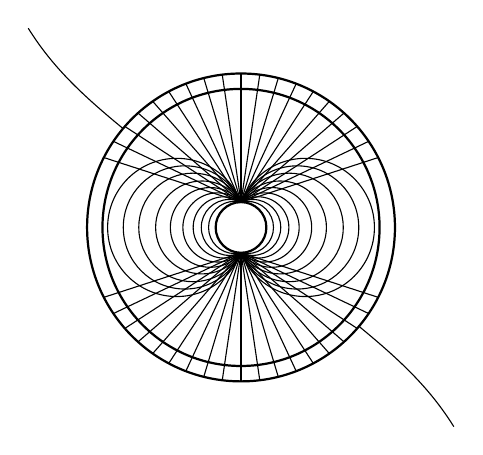
\begin{tikzpicture}[scale=1.15]
  % residual (weak) field lines leaking outside the shell
  \draw (-1.30,1.09) .. controls (-1.8,1.5) and (-2.1,1.8) .. (-2.35,2.2);
  \draw (1.30,-1.09) .. controls (1.8,-1.5) and (2.1,-1.8) .. (2.35,-2.2);
  % field lines looping around the wire pair inside the cavity
  % (circles through (0,+-0.28), i.e. the two wires hidden behind the
  %  central white circle)
  \foreach \c in {0.07,0.13,0.19,0.26,0.34,0.43,0.53,0.62,0.71}{
    \draw (\c,0) circle ({sqrt(\c*\c+0.0784)});
    \draw (-\c,0) circle ({sqrt(\c*\c+0.0784)});
  }
  % flux crossing the permeable shell at top and bottom (drawn inside the
  %  shell as nearly radial spokes)
  \foreach \t in {-63,-56,-49,-42,-35,-28,-21,-14,-7,0,7,14,21,28,35,42,49,56,63}{
    \draw (0,0.28) -- ({1.7*sin(\t)},{1.7*cos(\t)});
    \draw (0,-0.28) -- ({-1.7*sin(\t)},{-1.7*cos(\t)});
  }
  % steel shell
  \draw[thick] (0,0) circle (1.53);
  \draw[thick] (0,0) circle (1.7);
  % blank core covering the two wires
  \fill[white] (0,0) circle (0.28);
  \draw[thick] (0,0) circle (0.28);
\end{tikzpicture}
\par\vspace{0.5em}\textbf{Problem 5.15}
\end{center}
\solution
\textbf{(a)} Put $+I\widehat{\mathbf z}$ at $x=d/2$ and
$-I\widehat{\mathbf z}$ at $x=-d/2$. A straight wire has
$\mathbf H=(I/2\pi)\nabla\phi$, so a local scalar potential for the pair is
\[
\Phi_H=\frac I{2\pi}\{\arg(x+iy+d/2)-\arg(x+iy-d/2)\}.
\]
For $\rho\gg d$, expand the logarithms whose imaginary parts give the
arguments:
\[
\ln(w+d/2)-\ln(w-d/2)=\frac d w+\frac{d^3}{12w^3}+\cdots,
\qquad w=\rho e^{i\phi}.
\]
Consequently
\[
\boxed{\Phi_H=-\frac{Id}{2\pi\rho}\sin\phi
+O\!\left(I\frac{d^3}{\rho^3}\right).}
\]
The next term is actually odd in $d$ and of third order; the
second-order remainder quoted in the question is a looser estimate.

\textbf{(b)} Work to this dipole order, so $d\ll a$.
Set $p=Id/(2\pi)$, $\kappa=\mu_r$, $\eta=a^2/b^2$, and
$\Delta=(\kappa+1)^2-(\kappa-1)^2\eta$. Write
\[
\Phi_H=-p\sin\phi
\begin{cases}\rho^{-1}+A\rho,&0<\rho<a,\\
B\rho^{-1}+C\rho,&a<\rho<b,\\D\rho^{-1},&\rho>b.\end{cases}
\]
Continuity of potential and $\mu\partial_\rho\Phi_H$ gives
\[
1+Aa^2=B+Ca^2,\quad Aa^2-1=\kappa(Ca^2-B),\quad
B+Cb^2=D,\quad\kappa(Cb^2-B)=-D.
\]
The last pair gives $C=(\kappa-1)B/[(\kappa+1)b^2]$ and
$D=2\kappa B/(\kappa+1)$. The first pair then implies
$(\kappa+1)B-(\kappa-1)Ca^2=2$. Hence
\[
\boxed{A=-\frac{(\kappa^2-1)(1-\eta)}{\Delta a^2},\quad
B=\frac{2(\kappa+1)}{\Delta},\quad
C=\frac{2(\kappa-1)}{\Delta b^2},\quad
D=\frac{4\kappa}{\Delta}=F.}
\]
The exterior is the original two-dimensional dipole multiplied by $F$.
This is exactly the core-field transmission factor of 5.14, consistent
with reciprocity between a source inside and an applied field outside.
The singular central dipole represents the two wires only at distances
large compared with $d$.

\textbf{(c)} It is useful to rearrange the exact factor before expanding:
\[
F^{-1}=1+\frac{(\kappa-1)^2}{4\kappa}(1-a^2/b^2).
\]
For $t=b-a\ll b$,
$1-a^2/b^2=2t/b-t^2/b^2$, so for $\kappa\gg1$
\[
\boxed{F\simeq\frac1{1+\kappa t/(2b)}.}
\]
If also $\kappa t/(2b)\gg1$, this further reduces to $2b/(\kappa t)$.
With the specified numbers these estimates are $0.0400$ and $0.04167$,
respectively. The exact factor is $0.04564$, because $t/b=0.24$
is only moderately small. The exact suppression is about a factor
of $21.9$; the leading thin-shell estimate gives a factor of $25$.


\Needspace{5\baselineskip}
\par\bigskip
\noindent\textbf{5.16}\quad A circular loop of wire of radius $a$ and negligible thickness carries a current $I$. The loop is centered in a spherical cavity of radius $b>a$ in a large block of soft iron. Assume that the relative permeability of the iron is effectively infinite and that of the medium in the cavity, unity.
\begin{enumerate}
\item[(a)] In the approximation of $b\gg a$, show that the magnetic field at the center of the loop is augmented by a factor $(1+a^{3}/2b^{3})$ by the presence of the iron.
\item[(b)] What is the radius of the ``image'' current loop (carrying the same current) that simulates \erratum{the leading, nearly uniform reaction field of the iron for $r<b$, in the same $b\gg a$ approximation}? \erratum{Check whether a single such loop can reproduce the complete reaction field exactly.}
\end{enumerate}
\solution
\textbf{(a)} For $b\gg a$, the loop's field at the cavity wall is
dominated by its dipole moment $m=I\pi a^2$. The direct scalar potential
for $\mathbf H$ there is $m\cos\theta/(4\pi r^2)$.
Infinite permeability outside makes tangential $\mathbf H$ vanish
at $r=b$, so the wall must be an equipotential. The regular $l=1$
reaction potential that cancels its angular variation is
\[
\Phi_{H,\rm react}=-\frac{m}{4\pi b^3}r\cos\theta.
\]
Taking $-\mu_0\nabla$ gives the uniform reaction induction
$\mathbf B_{\rm react}=\mu_0m\widehat{\mathbf z}/(4\pi b^3)$.
Adding the exact free-loop center field $\mu_0I/(2a)$ gives
\[
\boxed{B_{\rm center}\simeq\frac{\mu_0I}{2a}
\left(1+\frac{a^3}{2b^3}\right).}
\]
Higher regular multipoles do not contribute at the exact center, so
this center value is in fact unchanged by retaining the other loop
multipoles; the dipole approximation is needed for the statement that
the reaction field is uniform throughout the cavity.

\textbf{(b)} A coaxial image loop carrying the same current $I$ has
center field $\mu_0I/(2R_{\rm im})$. Matching the leading uniform
reaction field gives
\[
\frac{\mu_0I}{2R_{\rm im}}=\frac{\mu_0Ia^2}{4b^3},\qquad
\boxed{R_{\rm im}=\frac{2b^3}{a^2}.}
\]
Since $R_{\rm im}\gg b$ when $b\gg a$, this image produces an almost
uniform field over the cavity.

It is not an exact image for all $r<b$ at arbitrary $a/b$.
Here is a direct check of that necessary qualification.
For an odd $l$, the real-loop exterior $A_\phi$ is proportional to
$\mu_l r^{-l-1}P_l^1$, while the regular reaction term is proportional
to $m_l^{\,R}r^lP_l^1$. The condition $B_\theta(b)=0$ requires
\[
\frac{m_l^{\,R}}{\mu_l}=\frac{l}{l+1}b^{-2l-1}.
\]
A single same-current image loop of radius $R$ instead has, from 5.8,
$m_l^{\,R}/\mu_l=R^{-l}a^{-l-1}$.
The $l=1$ condition demands $R=2b^3/a^2$, whereas $l=3$ demands
$R^3=4b^7/(3a^4)$. These cannot both hold for $b>a$:
their combination would require $b^2/a^2=1/6$.
Thus the equal-current image-loop statement must be understood in
the leading uniform-field approximation, as made explicit above.


\Needspace{5\baselineskip}
\par\bigskip
\noindent\textbf{5.17}\quad A current distribution $\mathbf{J}(\mathbf{x})$ exists in a medium of unit relative permeability adjacent to a semi-infinite slab of material having relative permeability $\mu_{r}$ and filling the half-space, $z<0$.
\begin{enumerate}
\item[(a)] Show that for $z>0$ the magnetic induction can be calculated by replacing the medium of permeability $\mu_{r}$ by an image current distribution, $\mathbf{J}^{*}$, with components,
\[
\left(\frac{\mu_{r}-1}{\mu_{r}+1}\right)\!J_{x}(x,y,-z),\qquad
\left(\frac{\mu_{r}-1}{\mu_{r}+1}\right)\!J_{y}(x,y,-z),\qquad
-\left(\frac{\mu_{r}-1}{\mu_{r}+1}\right)\!J_{z}(x,y,-z)
\]
\item[(b)] Show that for $z<0$ the magnetic induction appears to be due to a current distribution $[2\mu_{r}/(\mu_{r}+1)]\mathbf{J}$ in a medium of unit relative permeability.
\end{enumerate}
\solution
Let $\mathcal R=\operatorname{diag}(1,1,-1)$ reflect a vector across
the interface, and let $\mathbf B^{(0)}$ be the field of the original
current computed in vacuum everywhere.
Under spatial reflection a current is a polar vector but its magnetic
field is an axial vector. Direct substitution in Biot--Savart gives
\[
\mathbf J_{\rm ref}(\mathbf x)=\mathcal R\mathbf J(\mathcal R\mathbf x),
\qquad
\mathbf B_{\rm ref}(\mathbf x)=-\mathcal R\mathbf B^{(0)}(\mathcal R\mathbf x).
\]
In particular, at $z=0$ its tangential field reverses sign and its
normal field keeps its sign.

Take the upper field to be $\mathbf B^{(0)}+\chi\mathbf B_{\rm ref}$
and the lower field to be $T\mathbf B^{(0)}$. At the interface,
continuity of $B_n$ and $H_t$ requires
\[
1+\chi=T,\qquad 1-\chi=T/\mu_r.
\]
Solving gives $\chi=(\mu_r-1)/(\mu_r+1)$ and
$T=2\mu_r/(\mu_r+1)$.
Therefore
\[
\boxed{\mathbf J^*(x,y,z)=\frac{\mu_r-1}{\mu_r+1}
(J_x(x,y,-z),J_y(x,y,-z),-J_z(x,y,-z))}
\]
is the image distribution for part (a), and
\[
\boxed{\mathbf B_{z<0}=\frac{2\mu_r}{\mu_r+1}\mathbf B^{(0)}}
\]
proves part (b). Both candidate fields are divergence-free and satisfy
the correct source-free curl equations in their respective regions,
the interface conditions, and decay at infinity; uniqueness completes
the construction. At $\mu_r=1$ the image disappears and $T=1$.


\Needspace{5\baselineskip}
\par\bigskip
\noindent\textbf{5.18}\quad A circular loop of wire having a radius $a$ and carrying a current $I$ is located in vacuum with its center a distance $d$ away from a semi-infinite slab of permeability $\mu$. Find the force acting on the loop when
\begin{enumerate}
\item[(a)] the plane of the loop is parallel to the face of the slab,
\item[(b)] the plane of the loop is perpendicular to the face of the slab.
\item[(c)] Determine the limiting form of your answer to parts a and b when $d\gg a$. Can you obtain these limiting values in some simple and direct way?
\end{enumerate}
\solution
Choose the slab as $z<0$, the center as $(0,0,d)$, and write
$\chi=(\mu-\mu_0)/(\mu+\mu_0)$.
For each orientation the image is centered at $z=-d$. Let $s=2d$.
In computing the Lorentz force, the real loop moves in the field of
an image at its instantaneous position; one does not differentiate
that position a second time. Equivalently, the mechanical image
interaction energy carries a factor $1/2$.

\textbf{(a)} A loop parallel to the interface has a same-sense image
with current $\chi I$. For coaxial equal loops (derived in 5.28),
\[
M_\parallel(s)=\mu_0a\left[\left(\frac2k-k\right)K(k)-\frac2kE(k)\right],
\qquad k=\frac{2a}{\sqrt{4a^2+s^2}}.
\]
The force is purely normal, $F_z=\chi I^2M_\parallel'(s)$.
Using
$K'=E/[k(1-k^2)]-K/k$, $E'=(E-K)/k$, and
$dk/ds=-ks/(4a^2+s^2)$ gives
\[
\boxed{F_z=-\frac{\mu_0\chi I^2s k}{4a}
\left[\frac{2-k^2}{1-k^2}E(k)-2K(k)\right]_{s=2d}.}
\]
This holds for any $d>0$ in the ideal filament model.

\textbf{(b)} A perpendicular loop must have $d>a$ to lie wholly
in vacuum. Its image is coplanar with it and carries opposite-sense
current $-\chi I$. Define the positive coefficients
\[
D_n=\frac{[(2n+2)!]^2}
{2^{2n+2}n!(n+2)![(n+1)!]^2},\qquad
E_n=D_n\frac{(2n+2)!}{2^{2n+2}[(n+1)!]^2}.
\]
The convergent coplanar mutual inductance derived in 5.34 is
$M_\perp(s)=-\mu_0\pi a\sum_{n\ge0}E_n(a/s)^{2n+3}$.
Thus the exact force throughout the allowed domain $s=2d>2a$ is
\[
\boxed{F_z=-\chi I^2M_\perp'(2d)
=-\mu_0\pi\chi I^2\sum_{n=0}^\infty
(2n+3)E_n\left(\frac{a}{2d}\right)^{2n+4}.}
\]
All coefficients are positive, so the direction is toward a more
permeable slab and away from a less permeable one.
The two in-plane transverse force components cancel by symmetry.

\textbf{(c)} Expanding the preceding results, or using
$D_0=1/2$ and $E_0=1/4$, gives
\[
\boxed{F_{z,\parallel}\sim-\frac{3\mu_0\pi\chi I^2a^4}{32d^4},
\qquad F_{z,\perp}\sim-\frac{3\mu_0\pi\chi I^2a^4}{64d^4}.}
\]
For a direct dipole check, use $m=I\pi a^2$ and separation $s$.
Parallel-to-interface loops have axial moments $m,\chi m$:
$U_{\rm pair}=-2\mu_0\chi m^2/(4\pi s^3)$.
Perpendicular loops have transverse moments $m,-\chi m$:
$U_{\rm pair}=-\mu_0\chi m^2/(4\pi s^3)$.
The force on the real dipole is $-\partial_sU_{\rm pair}$.
Putting $s=2d$ gives the two boxed limits, with the first twice the second.


\Needspace{5\baselineskip}
\par\bigskip
\noindent\textbf{5.19}\quad A magnetically ``hard'' material is in the shape of a right circular cylinder of length $L$ and radius $a$. The cylinder has a permanent magnetization $M_{0}$, uniform throughout its volume and parallel to its axis.
\begin{enumerate}
\item[(a)] Determine the magnetic field $\mathbf{H}$ and magnetic induction $\mathbf{B}$ at all points on the axis of the cylinder, both inside and outside.
\item[(b)] Plot the ratios $\mathbf{B}/\mu_{0}M_{0}$ and $\mathbf{H}/M_{0}$ on the axis as functions of $z$ for $L/a=5$.
\end{enumerate}
\solution
\textbf{(a)} Let the cylinder occupy $-L/2<z<L/2$, with
$\mathbf M=M_0\widehat{\mathbf z}$.
Its volume bound current vanishes, and its curved surface carries
$\mathbf K_M=\mathbf M\times\widehat{\boldsymbol\rho}
=M_0\widehat{\boldsymbol\phi}$.
Thus its induction is that of the ideal finite solenoid in 5.3, with
$NI$ replaced by $M_0$. Define
\[
f(z)=\frac12\left[
\frac{z+L/2}{\sqrt{a^2+(z+L/2)^2}}
-\frac{z-L/2}{\sqrt{a^2+(z-L/2)^2}}\right].
\]
The answers on the entire axis, with one-sided limits at the end faces, are
\[
\boxed{\mathbf B(z)=\mu_0M_0f(z)\widehat{\mathbf z},\qquad
\mathbf H(z)=M_0[f(z)-\mathbf1_{\{|z|<L/2\}}]\widehat{\mathbf z}.}
\]
The subtraction follows from $\mathbf B=\mu_0(\mathbf H+\mathbf M)$.
The axial induction is continuous across either face, while $H_z$
jumps by the magnetic pole-sheet strength $M_0$.
\textbf{(b)} For $L/a=5$, at the center $f(0)=2.5/\sqrt{7.25}=0.928477$,
so $H_z(0)/M_0=-0.0715233$. At either end $f=\tfrac12(5/\sqrt{26})
=0.490290$.
\begin{center}
\begin{tikzpicture}[x=.8cm,y=2.5cm]
\draw[->] (-6.2,0)--(6.5,0) node[right] {$z/a$};
\draw[->] (-6,-.65)--(-6,1.2) node[above] {axial field};
\draw[blue,thick] plot coordinates {(-6.0000000,0.0158133) (-5.9500000,0.0163019) (-5.9000000,0.0168114) (-5.8500000,0.0173430) (-5.8000000,0.0178979) (-5.7500000,0.0184774) (-5.7000000,0.0190829) (-5.6500000,0.0197161) (-5.6000000,0.0203783) (-5.5500000,0.0210714) (-5.5000000,0.0217973) (-5.4500000,0.0225578) (-5.4000000,0.0233552) (-5.3500000,0.0241918) (-5.3000000,0.0250699) (-5.2500000,0.0259922) (-5.2000000,0.0269617) (-5.1500000,0.0279813) (-5.1000000,0.0290543) (-5.0500000,0.0301845) (-5.0000000,0.0313756) (-4.9500000,0.0326318) (-4.9000000,0.0339578) (-4.8500000,0.0353583) (-4.8000000,0.0368387) (-4.7500000,0.0384048) (-4.7000000,0.0400629) (-4.6500000,0.0418198) (-4.6000000,0.0436830) (-4.5500000,0.0456605) (-4.5000000,0.0477612) (-4.4500000,0.0499946) (-4.4000000,0.0523712) (-4.3500000,0.0549025) (-4.3000000,0.0576009) (-4.2500000,0.0604802) (-4.2000000,0.0635551) (-4.1500000,0.0668420) (-4.1000000,0.0703586) (-4.0500000,0.0741244) (-4.0000000,0.0781607) (-3.9500000,0.0824906) (-3.9000000,0.0871393) (-3.8500000,0.0921344) (-3.8000000,0.0975058) (-3.7500000,0.1032859) (-3.7000000,0.1095099) (-3.6500000,0.1162157) (-3.6000000,0.1234438) (-3.5500000,0.1312377) (-3.5000000,0.1396436) (-3.4500000,0.1487098) (-3.4000000,0.1584869) (-3.3500000,0.1690269) (-3.3000000,0.1803825) (-3.2500000,0.1926059) (-3.2000000,0.2057473) (-3.1500000,0.2198537) (-3.1000000,0.2349659) (-3.0500000,0.2511168) (-3.0000000,0.2683282) (-2.9500000,0.2866076) (-2.9000000,0.3059457) (-2.8500000,0.3263128) (-2.8000000,0.3476569) (-2.7500000,0.3699015) (-2.7000000,0.3929452) (-2.6500000,0.4166623) (-2.6000000,0.4409050) (-2.5500000,0.4655074) (-2.5000000,0.4902903) (-2.4500000,0.5150678) (-2.4000000,0.5396539) (-2.3500000,0.5638694) (-2.3000000,0.5875483) (-2.2500000,0.6105427) (-2.2000000,0.6327269) (-2.1500000,0.6539994) (-2.1000000,0.6742835) (-2.0500000,0.6935271) (-2.0000000,0.7117003) (-1.9500000,0.7287936) (-1.9000000,0.7448143) (-1.8500000,0.7597840) (-1.8000000,0.7737352) (-1.7500000,0.7867086) (-1.7000000,0.7987506) (-1.6500000,0.8099113) (-1.6000000,0.8202425) (-1.5500000,0.8297965) (-1.5000000,0.8386246) (-1.4500000,0.8467772) (-1.4000000,0.8543020) (-1.3500000,0.8612446) (-1.3000000,0.8676479) (-1.2500000,0.8735519) (-1.2000000,0.8789937) (-1.1500000,0.8840077) (-1.1000000,0.8886257) (-1.0500000,0.8928766) (-1.0000000,0.8967871) (-0.9500000,0.9003815) (-0.9000000,0.9036819) (-0.8500000,0.9067084) (-0.8000000,0.9094793) (-0.7500000,0.9120111) (-0.7000000,0.9143186) (-0.6500000,0.9164154) (-0.6000000,0.9183134) (-0.5500000,0.9200235) (-0.5000000,0.9215552) (-0.4500000,0.9229172) (-0.4000000,0.9241168) (-0.3500000,0.9251605) (-0.3000000,0.9260542) (-0.2500000,0.9268025) (-0.2000000,0.9274094) (-0.1500000,0.9278782) (-0.1000000,0.9282113) (-0.0500000,0.9284104) (0.0000000,0.9284767) (0.0500000,0.9284104) (0.1000000,0.9282113) (0.1500000,0.9278782) (0.2000000,0.9274094) (0.2500000,0.9268025) (0.3000000,0.9260542) (0.3500000,0.9251605) (0.4000000,0.9241168) (0.4500000,0.9229172) (0.5000000,0.9215552) (0.5500000,0.9200235) (0.6000000,0.9183134) (0.6500000,0.9164154) (0.7000000,0.9143186) (0.7500000,0.9120111) (0.8000000,0.9094793) (0.8500000,0.9067084) (0.9000000,0.9036819) (0.9500000,0.9003815) (1.0000000,0.8967871) (1.0500000,0.8928766) (1.1000000,0.8886257) (1.1500000,0.8840077) (1.2000000,0.8789937) (1.2500000,0.8735519) (1.3000000,0.8676479) (1.3500000,0.8612446) (1.4000000,0.8543020) (1.4500000,0.8467772) (1.5000000,0.8386246) (1.5500000,0.8297965) (1.6000000,0.8202425) (1.6500000,0.8099113) (1.7000000,0.7987506) (1.7500000,0.7867086) (1.8000000,0.7737352) (1.8500000,0.7597840) (1.9000000,0.7448143) (1.9500000,0.7287936) (2.0000000,0.7117003) (2.0500000,0.6935271) (2.1000000,0.6742835) (2.1500000,0.6539994) (2.2000000,0.6327269) (2.2500000,0.6105427) (2.3000000,0.5875483) (2.3500000,0.5638694) (2.4000000,0.5396539) (2.4500000,0.5150678) (2.5000000,0.4902903) (2.5500000,0.4655074) (2.6000000,0.4409050) (2.6500000,0.4166623) (2.7000000,0.3929452) (2.7500000,0.3699015) (2.8000000,0.3476569) (2.8500000,0.3263128) (2.9000000,0.3059457) (2.9500000,0.2866076) (3.0000000,0.2683282) (3.0500000,0.2511168) (3.1000000,0.2349659) (3.1500000,0.2198537) (3.2000000,0.2057473) (3.2500000,0.1926059) (3.3000000,0.1803825) (3.3500000,0.1690269) (3.4000000,0.1584869) (3.4500000,0.1487098) (3.5000000,0.1396436) (3.5500000,0.1312377) (3.6000000,0.1234438) (3.6500000,0.1162157) (3.7000000,0.1095099) (3.7500000,0.1032859) (3.8000000,0.0975058) (3.8500000,0.0921344) (3.9000000,0.0871393) (3.9500000,0.0824906) (4.0000000,0.0781607) (4.0500000,0.0741244) (4.1000000,0.0703586) (4.1500000,0.0668420) (4.2000000,0.0635551) (4.2500000,0.0604802) (4.3000000,0.0576009) (4.3500000,0.0549025) (4.4000000,0.0523712) (4.4500000,0.0499946) (4.5000000,0.0477612) (4.5500000,0.0456605) (4.6000000,0.0436830) (4.6500000,0.0418198) (4.7000000,0.0400629) (4.7500000,0.0384048) (4.8000000,0.0368387) (4.8500000,0.0353583) (4.9000000,0.0339578) (4.9500000,0.0326318) (5.0000000,0.0313756) (5.0500000,0.0301845) (5.1000000,0.0290543) (5.1500000,0.0279813) (5.2000000,0.0269617) (5.2500000,0.0259922) (5.3000000,0.0250699) (5.3500000,0.0241918) (5.4000000,0.0233552) (5.4500000,0.0225578) (5.5000000,0.0217973) (5.5500000,0.0210714) (5.6000000,0.0203783) (5.6500000,0.0197161) (5.7000000,0.0190829) (5.7500000,0.0184774) (5.8000000,0.0178979) (5.8500000,0.0173430) (5.9000000,0.0168114) (5.9500000,0.0163019) (6.0000000,0.0158133)};
\draw[red,thick,dashed] plot coordinates {(-6.0000000,0.0158133) (-5.9562500,0.0162397) (-5.9125000,0.0166820) (-5.8687500,0.0171410) (-5.8250000,0.0176174) (-5.7812500,0.0181122) (-5.7375000,0.0186263) (-5.6937500,0.0191605) (-5.6500000,0.0197161) (-5.6062500,0.0202939) (-5.5625000,0.0208952) (-5.5187500,0.0215211) (-5.4750000,0.0221731) (-5.4312500,0.0228524) (-5.3875000,0.0235606) (-5.3437500,0.0242992) (-5.3000000,0.0250699) (-5.2562500,0.0258744) (-5.2125000,0.0267147) (-5.1687500,0.0275928) (-5.1250000,0.0285109) (-5.0812500,0.0294713) (-5.0375000,0.0304764) (-4.9937500,0.0315290) (-4.9500000,0.0326318) (-4.9062500,0.0337880) (-4.8625000,0.0350009) (-4.8187500,0.0362738) (-4.7750000,0.0376106) (-4.7312500,0.0390154) (-4.6875000,0.0404926) (-4.6437500,0.0420467) (-4.6000000,0.0436830) (-4.5562500,0.0454068) (-4.5125000,0.0472239) (-4.4687500,0.0491408) (-4.4250000,0.0511643) (-4.3812500,0.0533017) (-4.3375000,0.0555609) (-4.2937500,0.0579507) (-4.2500000,0.0604802) (-4.2062500,0.0631595) (-4.1625000,0.0659994) (-4.1187500,0.0690117) (-4.0750000,0.0722091) (-4.0312500,0.0756051) (-3.9875000,0.0792147) (-3.9437500,0.0830537) (-3.9000000,0.0871393) (-3.8562500,0.0914901) (-3.8125000,0.0961259) (-3.7687500,0.1010683) (-3.7250000,0.1063401) (-3.6812500,0.1119660) (-3.6375000,0.1179721) (-3.5937500,0.1243862) (-3.5500000,0.1312377) (-3.5062500,0.1385577) (-3.4625000,0.1463786) (-3.4187500,0.1547339) (-3.3750000,0.1636583) (-3.3312500,0.1731869) (-3.2875000,0.1833550) (-3.2437500,0.1941973) (-3.2000000,0.2057473) (-3.1562500,0.2180361) (-3.1125000,0.2310916) (-3.0687500,0.2449369) (-3.0250000,0.2595891) (-2.9812500,0.2750579) (-2.9375000,0.2913437) (-2.8937500,0.3084361) (-2.8500000,0.3263128) (-2.8062500,0.3449378) (-2.7625000,0.3642610) (-2.7187500,0.3842176) (-2.6750000,0.4047283) (-2.6312500,0.4257003) (-2.5875000,0.4470287) (-2.5437500,0.4685992) (-2.5000000,0.4902903)};
\draw[red,thick,dashed] plot coordinates {(-2.5000000,-0.5097097) (-2.4375000,-0.4787606) (-2.3750000,-0.4481813) (-2.3125000,-0.4183127) (-2.2500000,-0.3894573) (-2.1875000,-0.3618661) (-2.1250000,-0.3357312) (-2.0625000,-0.3111843) (-2.0000000,-0.2882997) (-1.9375000,-0.2671013) (-1.8750000,-0.2475713) (-1.8125000,-0.2296592) (-1.7500000,-0.2132914) (-1.6875000,-0.1983786) (-1.6250000,-0.1848226) (-1.5625000,-0.1725220) (-1.5000000,-0.1613754) (-1.4375000,-0.1512846) (-1.3750000,-0.1421567) (-1.3125000,-0.1339046) (-1.2500000,-0.1264481) (-1.1875000,-0.1197140) (-1.1250000,-0.1136356) (-1.0625000,-0.1081532) (-1.0000000,-0.1032129) (-0.9375000,-0.0987667) (-0.8750000,-0.0947718) (-0.8125000,-0.0911904) (-0.7500000,-0.0879889) (-0.6875000,-0.0851379) (-0.6250000,-0.0826115) (-0.5625000,-0.0803869) (-0.5000000,-0.0784448) (-0.4375000,-0.0767680) (-0.3750000,-0.0753423) (-0.3125000,-0.0741554) (-0.2500000,-0.0731975) (-0.1875000,-0.0724606) (-0.1250000,-0.0719384) (-0.0625000,-0.0716269) (0.0000000,-0.0715233) (0.0625000,-0.0716269) (0.1250000,-0.0719384) (0.1875000,-0.0724606) (0.2500000,-0.0731975) (0.3125000,-0.0741554) (0.3750000,-0.0753423) (0.4375000,-0.0767680) (0.5000000,-0.0784448) (0.5625000,-0.0803869) (0.6250000,-0.0826115) (0.6875000,-0.0851379) (0.7500000,-0.0879889) (0.8125000,-0.0911904) (0.8750000,-0.0947718) (0.9375000,-0.0987667) (1.0000000,-0.1032129) (1.0625000,-0.1081532) (1.1250000,-0.1136356) (1.1875000,-0.1197140) (1.2500000,-0.1264481) (1.3125000,-0.1339046) (1.3750000,-0.1421567) (1.4375000,-0.1512846) (1.5000000,-0.1613754) (1.5625000,-0.1725220) (1.6250000,-0.1848226) (1.6875000,-0.1983786) (1.7500000,-0.2132914) (1.8125000,-0.2296592) (1.8750000,-0.2475713) (1.9375000,-0.2671013) (2.0000000,-0.2882997) (2.0625000,-0.3111843) (2.1250000,-0.3357312) (2.1875000,-0.3618661) (2.2500000,-0.3894573) (2.3125000,-0.4183127) (2.3750000,-0.4481813) (2.4375000,-0.4787606) (2.5000000,-0.5097097)};
\draw[red,thick,dashed] plot coordinates {(2.5000000,0.4902903) (2.5437500,0.4685992) (2.5875000,0.4470287) (2.6312500,0.4257003) (2.6750000,0.4047283) (2.7187500,0.3842176) (2.7625000,0.3642610) (2.8062500,0.3449378) (2.8500000,0.3263128) (2.8937500,0.3084361) (2.9375000,0.2913437) (2.9812500,0.2750579) (3.0250000,0.2595891) (3.0687500,0.2449369) (3.1125000,0.2310916) (3.1562500,0.2180361) (3.2000000,0.2057473) (3.2437500,0.1941973) (3.2875000,0.1833550) (3.3312500,0.1731869) (3.3750000,0.1636583) (3.4187500,0.1547339) (3.4625000,0.1463786) (3.5062500,0.1385577) (3.5500000,0.1312377) (3.5937500,0.1243862) (3.6375000,0.1179721) (3.6812500,0.1119660) (3.7250000,0.1063401) (3.7687500,0.1010683) (3.8125000,0.0961259) (3.8562500,0.0914901) (3.9000000,0.0871393) (3.9437500,0.0830537) (3.9875000,0.0792147) (4.0312500,0.0756051) (4.0750000,0.0722091) (4.1187500,0.0690117) (4.1625000,0.0659994) (4.2062500,0.0631595) (4.2500000,0.0604802) (4.2937500,0.0579507) (4.3375000,0.0555609) (4.3812500,0.0533017) (4.4250000,0.0511643) (4.4687500,0.0491408) (4.5125000,0.0472239) (4.5562500,0.0454068) (4.6000000,0.0436830) (4.6437500,0.0420467) (4.6875000,0.0404926) (4.7312500,0.0390154) (4.7750000,0.0376106) (4.8187500,0.0362738) (4.8625000,0.0350009) (4.9062500,0.0337880) (4.9500000,0.0326318) (4.9937500,0.0315290) (5.0375000,0.0304764) (5.0812500,0.0294713) (5.1250000,0.0285109) (5.1687500,0.0275928) (5.2125000,0.0267147) (5.2562500,0.0258744) (5.3000000,0.0250699) (5.3437500,0.0242992) (5.3875000,0.0235606) (5.4312500,0.0228524) (5.4750000,0.0221731) (5.5187500,0.0215211) (5.5625000,0.0208952) (5.6062500,0.0202939) (5.6500000,0.0197161) (5.6937500,0.0191605) (5.7375000,0.0186263) (5.7812500,0.0181122) (5.8250000,0.0176174) (5.8687500,0.0171410) (5.9125000,0.0166820) (5.9562500,0.0162397) (6.0000000,0.0158133)};
\foreach \z in {-2.5,2.5} \draw[dotted] (\z,-.55)--(\z,1);
\foreach \z in {-5,-2.5,0,2.5,5} \node[below] at (\z,0) {$\z$};
\node[blue] at (0,1.13) {$B_z/(\mu_0M_0)$};
\node[red] at (0,-.45) {$H_z/M_0$};
\end{tikzpicture}

\end{center}
The red interior field opposes the magnetization; outside,
$\mathbf B/\mu_0=\mathbf H$ as required in vacuum.


\Needspace{5\baselineskip}
\par\bigskip
\noindent\textbf{5.20}\quad\begin{enumerate}
\item[(a)] Starting from the force equation (5.12) and the fact that a magnetization $\mathbf{M}$ inside a volume $V$ bounded by a surface $S$ is equivalent to a volume current density $\mathbf{J}_{M}=(\nabla\times\mathbf{M})$ and a surface current density $(\mathbf{M}\times\mathbf{n})$, show that in the absence of macroscopic conduction currents the total magnetic force on the body can be written
\[
\mathbf{F}=-\int_{V}(\nabla\cdot\mathbf{M})\mathbf{B}_{e}\;d^{3}x+\int_{S}(\mathbf{M}\cdot\mathbf{n})\mathbf{B}_{e}\;da
\]
where $\mathbf{B}_{e}$ is the applied magnetic induction (not including that of the body in question). The force is now expressed in terms of the effective charge densities $\rho_{M}$ and $\sigma_{M}$. If the distribution of magnetization is not discontinuous, the surface can be at infinity and the force given by just the volume integral.
\item[(b)] A sphere of radius $R$ with uniform magnetization has its center at the origin of coordinates and its direction of magnetization making spherical angles $\theta_{0}$, $\phi_{0}$. If the external magnetic field is the same as in Problem 5.11, use the expression of part a to evaluate the components of the force acting on the sphere.
\end{enumerate}
\solution
\textbf{(a)} The external sources are outside the body, so
$\nabla\times\mathbf B_e=0$ and $\nabla\cdot\mathbf B_e=0$ in its
neighborhood. Start from both bound-current contributions:
\[
\mathbf F=\int_V(\nabla\times\mathbf M)\times\mathbf B_e\,d^3x
+\oint_S(\mathbf M\times\mathbf n)\times\mathbf B_e\,da.
\]
The volume integrand has components
$B_{e,j}\partial_jM_i-B_{e,j}\partial_iM_j$.
Integrating both derivatives by parts gives the boundary term
$M_i(\mathbf B_e\cdot\mathbf n)-n_i(\mathbf M\cdot\mathbf B_e)$
and the volume term
$M_j\partial_iB_{e,j}-M_i\partial_jB_{e,j}$.
The surface-current term cancels the boundary term exactly.
Zero divergence removes its second volume term, leaving
\[
F_i=\int_VM_j\partial_iB_{e,j}\,d^3x.
\]
Zero curl allows $\partial_iB_{e,j}=\partial_jB_{e,i}$.
A final integration by parts then gives
\[
\boxed{\mathbf F=-\int_V(\nabla\cdot\mathbf M)\mathbf B_e\,d^3x
+\oint_S(\mathbf M\cdot\mathbf n)\mathbf B_e\,da.}
\]
These are effective pole densities $\rho_M=-\nabla\cdot\mathbf M$
and $\sigma_M=\mathbf M\cdot\mathbf n$.
If imposed external current overlaps $V$, zero curl is unavailable:
the additional force term is $\int_V\mathbf M\times(\nabla\times\mathbf B_e)d^3x$.

\textbf{(b)} For uniform $\mathbf M$ the volume pole density is zero.
On the sphere $\sigma_M=M_jn_j$, and the constant part of the external
field integrates to zero because $\int\mathbf n\,da=0$.
For its linear part, $x_k=Rn_k$ and
$\int n_jn_k\,da=(4\pi R^2/3)\delta_{jk}$, so
\[
F_i=R\,\partial_kB_{e,i}\,M_j\int n_jn_k\,da
=\frac{4\pi R^3}{3}M_j\partial_jB_{e,i}.
\]
With the field of 5.11 this gives
\[
\boxed{\mathbf F=\frac{4\pi R^3}{3}\beta B_0M\sin\theta_0
(\sin\phi_0,\cos\phi_0,0).}
\]
It equals the loop result with
$\mathbf m=(4\pi R^3/3)\mathbf M$, as expected for an affine field.


\Needspace{5\baselineskip}
\par\bigskip
\noindent\textbf{5.21}\quad A magnetostatic field is due entirely to a localized distribution of permanent magnetization.
\begin{enumerate}
\item[(a)] Show that
\[
\int\mathbf{B}\cdot\mathbf{H}\;d^{3}x=0
\]
provided the integral is taken over all space.
\item[(b)] From the potential energy (5.72) of a dipole in an external field, show that for a continuous distribution of permanent magnetization the magnetostatic energy can be written
\[
W=\frac{\mu_{0}}{2}\int\mathbf{H}\cdot\mathbf{H}\;d^{3}x=-\frac{\mu_{0}}{2}\int\mathbf{M}\cdot\mathbf{H}\;d^{3}x
\]
apart from an additive constant, which is independent of the orientation or position of the various constituent magnetized bodies.
\end{enumerate}
\solution
\textbf{(a)} With no free currents,
$\mathbf H=-\nabla\Phi_H$ throughout space. Therefore
\[
\int\mathbf B\cdot\mathbf H\,d^3x
=-\int\nabla\cdot(\Phi_H\mathbf B)d^3x
+\int\Phi_H\nabla\cdot\mathbf B\,d^3x=0.
\]
The volume term vanishes by $\nabla\cdot\mathbf B=0$.
For a localized magnetization, $\Phi_H=O(r^{-2})$ and
$B=O(r^{-3})$, so the surface term at infinity is $O(r^{-3})$ and
vanishes. Internal interfaces cancel when all space is included.

\textbf{(b)} The pair interaction energy of permanent dipoles is
$-\mathbf m\cdot\mathbf B_e$. Summing it over the distribution and
dividing by two to count each pair once gives
$-\tfrac12\int\mathbf M\cdot\mathbf B\,d^3x$, apart from local
self-energy terms. Since $\mathbf B=\mu_0(\mathbf H+\mathbf M)$,
\[
-\frac12\int\mathbf M\cdot\mathbf B
=-\frac{\mu_0}{2}\int\mathbf M\cdot\mathbf H
-\frac{\mu_0}{2}\int M^2.
\]
The last term and the local self-energy constants are unchanged by
translations or rotations of permanently magnetized bodies.
They may be absorbed into the additive constant specified in the question.
Part (a) also gives
\[
0=\mu_0\int(\mathbf H+\mathbf M)\cdot\mathbf H\,d^3x,
\quad\text{hence}\quad
\int H^2=-\int\mathbf M\cdot\mathbf H.
\]
Consequently the position- and orientation-dependent energy can be written
\[
\boxed{W=\frac{\mu_0}{2}\int H^2d^3x
=-\frac{\mu_0}{2}\int\mathbf M\cdot\mathbf H\,d^3x+\text{constant}.}
\]
The moment magnitudes are fixed here; changing them would change the
discarded intrinsic energy and would be a different thermodynamic problem.


\Needspace{5\baselineskip}
\par\bigskip
\noindent\textbf{5.22}\quad Show that in general a long, straight bar of uniform cross-sectional area $A$ with uniform lengthwise magnetization $M$, when placed with its flat end against an infinitely permeable flat surface, adheres with a force given approximately by
\[
F\simeq\frac{\mu_{0}}{2}\,AM^{2}
\]
Relate your discussion to the electrostatic considerations in Section 1.11.
\solution
Resolve contact as the limit of a narrow vacuum gap. The end face has
effective magnetic surface charge of magnitude $M$.
Infinite permeability can be represented by an image magnet extending
the real bar through the plane; the facing image pole has opposite sign.
For a bar long compared with its transverse size, the far ends make
negligible contributions in the gap. Each facing pole sheet supplies
$H=M/2$, so the total gap field is $H=M$, $B=\mu_0M$.

The force on the real face is its pole strength $MA$ times the
\emph{image} induction $\mu_0M/2$, giving
\[
\boxed{F\simeq\frac{\mu_0}{2}AM^2.}
\]
The same result follows from the normal vacuum magnetic stress
$B^2/(2\mu_0)$ times $A$. In the electrostatic capacitor the corresponding
pressure is $\epsilon_0E^2/2=\sigma^2/(2\epsilon_0)$.
Using the field of both sheets as the acting external field would
incorrectly double the force; the face does not exert a net force on itself.


\Needspace{5\baselineskip}
\par\bigskip
\noindent\textbf{5.23}\quad A right circular cylinder of length $L$ and radius $a$ has a uniform lengthwise magnetization $M$.
\begin{enumerate}
\item[(a)] Show that, when it is placed with its flat end against an infinitely permeable plane surface, it adheres with a force
\[
F=2\mu_{0}aLM^{2}\left[\frac{K(k)-E(k)}{k}-\frac{K(k_{1})-E(k_{1})}{k_{1}}\right]
\]
where
\[
k=\frac{2a}{\sqrt{4a^{2}+L^{2}}},\qquad k_{1}=\frac{a}{\sqrt{a^{2}+L^{2}}}
\]
\item[(b)] Find the limiting form for the force if $L\gg a$.
\end{enumerate}
\solution
\textbf{(a)} Use magnetic pole disks $\pm M$ at the two end faces and
the image cylinder across the infinitely permeable plane.
Let $f(s)>0$ be the attraction of two oppositely charged disks of
radius $a$, density magnitudes $M$, and axial separation $s$.
Biot--Savart's equivalent pole force is
\[
f(s)=\frac{\mu_0M^2}{4\pi}\int_Dd^2x\int_Dd^2x'
\frac{s}{[s^2+|\mathbf x-\mathbf x'|^2]^{3/2}}.
\]
The overlap area of disks displaced transversely by $t$ is
\[
C(t)=2a^2\cos^{-1}(t/2a)-\frac t2\sqrt{4a^2-t^2},\quad
0\le t\le2a,\qquad C'(t)=-\sqrt{4a^2-t^2}.
\]
Integrating by the displacement variable, then by parts, yields
\[
\begin{split}
f(s)&=\frac{\mu_0M^2}{2}\int_0^{2a}
C(t)\frac{st\,dt}{(s^2+t^2)^{3/2}}\\
&=\frac{\mu_0M^2}{2}\left[
\pi a^2-s\int_0^{2a}\frac{\sqrt{4a^2-t^2}}{\sqrt{s^2+t^2}}dt\right].
\end{split}
\]
For the remaining integral put $t=2a\cos u$ and
$k_s=2a/\sqrt{4a^2+s^2}$. It becomes
\[
\frac{4a^2}{\sqrt{4a^2+s^2}}\int_0^{\pi/2}
\frac{\sin^2u\,du}{\sqrt{1-k_s^2\sin^2u}}
=\frac{2a}{k_s}[K(k_s)-E(k_s)].
\]
Thus
$f(s)=\mu_0M^2\{\pi a^2/2-as[K(k_s)-E(k_s)]/k_s\}$.
In particular $f(0^+)=\mu_0M^2\pi a^2/2$.

The four real-image pairs give attraction $f(0)$ and $f(2L)$,
and two repulsions $f(L)$. Hence
\[
F=f(0)-2f(L)+f(2L)
=\boxed{2\mu_0aLM^2\left[
\frac{K(k)-E(k)}k-\frac{K(k_1)-E(k_1)}{k_1}\right]},
\]
with $k=k_L$ and $k_1=k_{2L}$ exactly as in the question.

\textbf{(b)} At small $k$,
$K=\frac\pi2(1+k^2/4+\cdots)$ and
$E=\frac\pi2(1-k^2/4+\cdots)$, so $(K-E)/k=\pi k/4+O(k^3)$.
When $L\gg a$, $k\simeq2a/L$ and $k_1\simeq a/L$, giving
\[
\boxed{F\longrightarrow \frac{\mu_0\pi a^2M^2}{2}.}
\]
This agrees with 5.22 for $A=\pi a^2$.


\Needspace{5\baselineskip}
\par\bigskip
\noindent\textbf{5.24}\quad\begin{enumerate}
\item[(a)] For the perfectly conducting plane of Section 5.13 with the circular hole in it and the asymptotically uniform tangential magnetic field $\mathbf{H}_{0}$ on one side, calculate the added tangential magnetic field $\mathbf{H}^{(1)}$ on the side of the plane with $\mathbf{H}_{0}$. Show that its components for $\rho>a$ are
\begin{align*}
H_{x}^{(1)}&=\frac{2H_{0}a^{3}}{\pi}\frac{xy}{\rho^{4}\sqrt{\rho^{2}-a^{2}}}\\[4pt]
H_{y}^{(1)}&=\frac{2H_{0}a^{3}}{\pi}\frac{y^{2}}{\rho^{4}\sqrt{\rho^{2}-a^{2}}}+\frac{H_{0}}{\pi}\left[\frac{a}{\rho}\sqrt{1-\frac{a^{2}}{\rho^{2}}}-\sin^{-1}\!\left(\frac{a}{\rho}\right)\right]
\end{align*}
\item[(b)] Sketch the lines of surface current flow in the neighborhood of the hole on both sides of the plane.
\end{enumerate}
\solution
Take $\mathbf H_0=H_0\widehat{\mathbf y}$ on the $z>0$ side.
The scalar potentials in Section 5.13 are
$\Phi_+=-H_0y+\Phi_1$ and $\Phi_-=-\Phi_1$, with
\[
\Phi_1=\frac{2H_0a^2}{\pi}\sin\phi
\int_0^\infty j_1(ka)e^{-k|z|}J_1(k\rho)\,dk.
\]
We evaluate its plane value rather than leaving a Bessel integral.
The identity
$a^2j_1(ka)=\int_0^a t\sin(kt)\,dt$, followed by integration by parts
in $k$, gives, for $t<\rho$,
\[
\int_0^\infty\sin(kt)J_1(k\rho)\,dk
=\frac t\rho\int_0^\infty\cos(kt)J_0(k\rho)\,dk
=\frac{t}{\rho\sqrt{\rho^2-t^2}}.
\]
These oscillatory integrals are understood as limits with positive
exponential damping, consistent with $z\to0^+$.
Consequently, for $\rho>a$,
\[
\int_0^\infty j_1(ka)J_1(k\rho)\,dk
=\frac1{a^2\rho}\int_0^a\frac{t^2\,dt}{\sqrt{\rho^2-t^2}}
=\frac{\rho}{2a^2}f(\rho),
\]
where
$f(\rho)=\sin^{-1}(a/\rho)-(a/\rho)\sqrt{1-a^2/\rho^2}$.
Thus $\Phi_1(x,y,0)=H_0yf(\rho)/\pi$.

\textbf{(a)} Differentiate explicitly:
\[
f'(\rho)=-\frac{2a^3}{\rho^3\sqrt{\rho^2-a^2}},\qquad
\partial_x\rho=x/\rho,\quad\partial_y\rho=y/\rho.
\]
Therefore
\[
\boxed{H_x^{(1)}=-\frac{H_0}{\pi}y f'(\rho)\frac x\rho
=\frac{2H_0a^3}{\pi}\frac{xy}{\rho^4\sqrt{\rho^2-a^2}},}
\]
\[
\boxed{H_y^{(1)}=-\frac{H_0}{\pi}
\left[f(\rho)+\frac{y^2}{\rho}f'(\rho)\right]
=\frac{2H_0a^3y^2}{\pi\rho^4\sqrt{\rho^2-a^2}}
+\frac{H_0}{\pi}
\left[\frac a\rho\sqrt{1-\frac{a^2}{\rho^2}}-\sin^{-1}\frac a\rho\right].}
\]
\textbf{(b)} On the upper face the outward normal from the conductor
is $+\widehat{\mathbf z}$ and on the lower face it is
$-\widehat{\mathbf z}$. Hence
\[
\mathbf K_+=-\!H_0\widehat{\mathbf x}
+\widehat{\mathbf z}\times\mathbf H^{(1)},\qquad
\mathbf K_-=\widehat{\mathbf z}\times\mathbf H^{(1)}.
\]
If $\psi_+=-y+yf/\pi$ and $\psi_-=yf/\pi$, both currents can be written
$\mathbf K_\pm/H_0=(\partial_y\psi_\pm,-\partial_x\psi_\pm)$.
Their streamlines are therefore contours of the respective $\psi$.
At the rim $f(a)=\pi/2$; the currents on the two faces join around
the edge, whereas there is no conducting sheet in the open disk.
\begin{center}
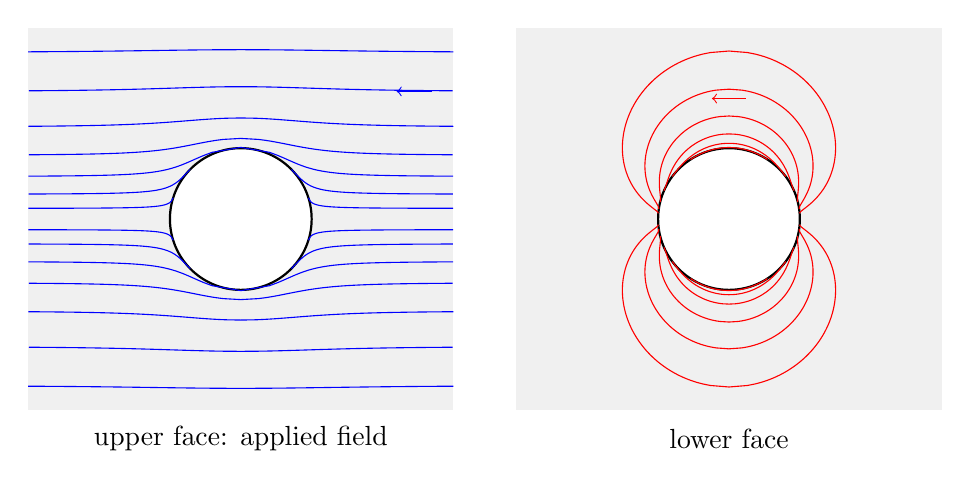
\begin{tikzpicture}[x=.9cm,y=.9cm]
\begin{scope}[xshift=0.0cm]
\fill[gray!12] (-3,-2.7) rectangle (3,2.7);
\filldraw[fill=white,draw=black,thick] (0,0) circle (1);
\draw[blue,thin] plot coordinates {(0.9539392,-0.3000000) (0.9827902,-0.2484115) (1.0007094,-0.2326496) (1.0170875,-0.2222917) (1.0327382,-0.2145772) (1.0479593,-0.2084680) (1.0628964,-0.2034460) (1.0776319,-0.1992115) (1.0922173,-0.1955741) (1.1066867,-0.1924049) (1.1210642,-0.1896123) (1.1353672,-0.1871287) (1.1496086,-0.1849029) (1.1637985,-0.1828951) (1.1779447,-0.1810739) (1.1920535,-0.1794136) (1.2061298,-0.1778937) (1.2201778,-0.1764969) (1.2342009,-0.1752088) (1.2482021,-0.1740174) (1.2621837,-0.1729122) (1.2761477,-0.1718844) (1.2900960,-0.1709264) (1.3040301,-0.1700315) (1.3179512,-0.1691939) (1.3318607,-0.1684084) (1.3457594,-0.1676706) (1.3596483,-0.1669765) (1.3735282,-0.1663224) (1.3873997,-0.1657053) (1.4012636,-0.1651222) (1.4151204,-0.1645706) (1.4289705,-0.1640482) (1.4428145,-0.1635528) (1.4566527,-0.1630826) (1.4704856,-0.1626359) (1.4843135,-0.1622110) (1.4981367,-0.1618065) (1.5119554,-0.1614212) (1.5257700,-0.1610538) (1.5395807,-0.1607031) (1.5533877,-0.1603683) (1.5671913,-0.1600482) (1.5809915,-0.1597421) (1.5947886,-0.1594491) (1.6085827,-0.1591686) (1.6223740,-0.1588997) (1.6361627,-0.1586419) (1.6499488,-0.1583946) (1.6637324,-0.1581571) (1.6775138,-0.1579291) (1.6912930,-0.1577099) (1.7050700,-0.1574991) (1.7188451,-0.1572964) (1.7326182,-0.1571013) (1.7463895,-0.1569135) (1.7601590,-0.1567325) (1.7739268,-0.1565581) (1.7876930,-0.1563899) (1.8014576,-0.1562277) (1.8152207,-0.1560712) (1.8289824,-0.1559201) (1.8427427,-0.1557742) (1.8565016,-0.1556333) (1.8702593,-0.1554970) (1.8840157,-0.1553654) (1.8977709,-0.1552380) (1.9115250,-0.1551148) (1.9252779,-0.1549956) (1.9390298,-0.1548802) (1.9527806,-0.1547684) (1.9665304,-0.1546601) (1.9802792,-0.1545552) (1.9940271,-0.1544536) (2.0077741,-0.1543550) (2.0215201,-0.1542594) (2.0352654,-0.1541667) (2.0490097,-0.1540767) (2.0627533,-0.1539894) (2.0764961,-0.1539047) (2.0902381,-0.1538223) (2.1039794,-0.1537424) (2.1177199,-0.1536647) (2.1314598,-0.1535892) (2.1451990,-0.1535159) (2.1589375,-0.1534445) (2.1726753,-0.1533752) (2.1864126,-0.1533077) (2.2001492,-0.1532421) (2.2138852,-0.1531782) (2.2276207,-0.1531160) (2.2413556,-0.1530555) (2.2550899,-0.1529966) (2.2688237,-0.1529392) (2.2825570,-0.1528833) (2.2962897,-0.1528289) (2.3100220,-0.1527758) (2.3237538,-0.1527241) (2.3374851,-0.1526737) (2.3512159,-0.1526245) (2.3649463,-0.1525766) (2.3786763,-0.1525299) (2.3924058,-0.1524843) (2.4061349,-0.1524398) (2.4198635,-0.1523964) (2.4335918,-0.1523540) (2.4473197,-0.1523126) (2.4610472,-0.1522723) (2.4747743,-0.1522328) (2.4885010,-0.1521943) (2.5022274,-0.1521567) (2.5159534,-0.1521200) (2.5296791,-0.1520841) (2.5434044,-0.1520490) (2.5571294,-0.1520148) (2.5708540,-0.1519812) (2.5845784,-0.1519485) (2.5983024,-0.1519165) (2.6120261,-0.1518851) (2.6257496,-0.1518545) (2.6394727,-0.1518246) (2.6531955,-0.1517952) (2.6669181,-0.1517666) (2.6806403,-0.1517385) (2.6943623,-0.1517111) (2.7080841,-0.1516842) (2.7218055,-0.1516579) (2.7355267,-0.1516321) (2.7492477,-0.1516069) (2.7629684,-0.1515822) (2.7766888,-0.1515580) (2.7904090,-0.1515343) (2.8041290,-0.1515111) (2.8178487,-0.1514884) (2.8315682,-0.1514661) (2.8452875,-0.1514443) (2.8590066,-0.1514229) (2.8727254,-0.1514020) (2.8864440,-0.1513814) (2.9001625,-0.1513613) (2.9138807,-0.1513415) (2.9275987,-0.1513221) (2.9413165,-0.1513032) (2.9550341,-0.1512845) (2.9687515,-0.1512663) (2.9824687,-0.1512483) (2.9961858,-0.1512308)};
\draw[blue,thin] plot coordinates {(-0.9539392,-0.3000000) (-0.9827902,-0.2484115) (-1.0007094,-0.2326496) (-1.0170875,-0.2222917) (-1.0327382,-0.2145772) (-1.0479593,-0.2084680) (-1.0628964,-0.2034460) (-1.0776319,-0.1992115) (-1.0922173,-0.1955741) (-1.1066867,-0.1924049) (-1.1210642,-0.1896123) (-1.1353672,-0.1871287) (-1.1496086,-0.1849029) (-1.1637985,-0.1828951) (-1.1779447,-0.1810739) (-1.1920535,-0.1794136) (-1.2061298,-0.1778937) (-1.2201778,-0.1764969) (-1.2342009,-0.1752088) (-1.2482021,-0.1740174) (-1.2621837,-0.1729122) (-1.2761477,-0.1718844) (-1.2900960,-0.1709264) (-1.3040301,-0.1700315) (-1.3179512,-0.1691939) (-1.3318607,-0.1684084) (-1.3457594,-0.1676706) (-1.3596483,-0.1669765) (-1.3735282,-0.1663224) (-1.3873997,-0.1657053) (-1.4012636,-0.1651222) (-1.4151204,-0.1645706) (-1.4289705,-0.1640482) (-1.4428145,-0.1635528) (-1.4566527,-0.1630826) (-1.4704856,-0.1626359) (-1.4843135,-0.1622110) (-1.4981367,-0.1618065) (-1.5119554,-0.1614212) (-1.5257700,-0.1610538) (-1.5395807,-0.1607031) (-1.5533877,-0.1603683) (-1.5671913,-0.1600482) (-1.5809915,-0.1597421) (-1.5947886,-0.1594491) (-1.6085827,-0.1591686) (-1.6223740,-0.1588997) (-1.6361627,-0.1586419) (-1.6499488,-0.1583946) (-1.6637324,-0.1581571) (-1.6775138,-0.1579291) (-1.6912930,-0.1577099) (-1.7050700,-0.1574991) (-1.7188451,-0.1572964) (-1.7326182,-0.1571013) (-1.7463895,-0.1569135) (-1.7601590,-0.1567325) (-1.7739268,-0.1565581) (-1.7876930,-0.1563899) (-1.8014576,-0.1562277) (-1.8152207,-0.1560712) (-1.8289824,-0.1559201) (-1.8427427,-0.1557742) (-1.8565016,-0.1556333) (-1.8702593,-0.1554970) (-1.8840157,-0.1553654) (-1.8977709,-0.1552380) (-1.9115250,-0.1551148) (-1.9252779,-0.1549956) (-1.9390298,-0.1548802) (-1.9527806,-0.1547684) (-1.9665304,-0.1546601) (-1.9802792,-0.1545552) (-1.9940271,-0.1544536) (-2.0077741,-0.1543550) (-2.0215201,-0.1542594) (-2.0352654,-0.1541667) (-2.0490097,-0.1540767) (-2.0627533,-0.1539894) (-2.0764961,-0.1539047) (-2.0902381,-0.1538223) (-2.1039794,-0.1537424) (-2.1177199,-0.1536647) (-2.1314598,-0.1535892) (-2.1451990,-0.1535159) (-2.1589375,-0.1534445) (-2.1726753,-0.1533752) (-2.1864126,-0.1533077) (-2.2001492,-0.1532421) (-2.2138852,-0.1531782) (-2.2276207,-0.1531160) (-2.2413556,-0.1530555) (-2.2550899,-0.1529966) (-2.2688237,-0.1529392) (-2.2825570,-0.1528833) (-2.2962897,-0.1528289) (-2.3100220,-0.1527758) (-2.3237538,-0.1527241) (-2.3374851,-0.1526737) (-2.3512159,-0.1526245) (-2.3649463,-0.1525766) (-2.3786763,-0.1525299) (-2.3924058,-0.1524843) (-2.4061349,-0.1524398) (-2.4198635,-0.1523964) (-2.4335918,-0.1523540) (-2.4473197,-0.1523126) (-2.4610472,-0.1522723) (-2.4747743,-0.1522328) (-2.4885010,-0.1521943) (-2.5022274,-0.1521567) (-2.5159534,-0.1521200) (-2.5296791,-0.1520841) (-2.5434044,-0.1520490) (-2.5571294,-0.1520148) (-2.5708540,-0.1519812) (-2.5845784,-0.1519485) (-2.5983024,-0.1519165) (-2.6120261,-0.1518851) (-2.6257496,-0.1518545) (-2.6394727,-0.1518246) (-2.6531955,-0.1517952) (-2.6669181,-0.1517666) (-2.6806403,-0.1517385) (-2.6943623,-0.1517111) (-2.7080841,-0.1516842) (-2.7218055,-0.1516579) (-2.7355267,-0.1516321) (-2.7492477,-0.1516069) (-2.7629684,-0.1515822) (-2.7766888,-0.1515580) (-2.7904090,-0.1515343) (-2.8041290,-0.1515111) (-2.8178487,-0.1514884) (-2.8315682,-0.1514661) (-2.8452875,-0.1514443) (-2.8590066,-0.1514229) (-2.8727254,-0.1514020) (-2.8864440,-0.1513814) (-2.9001625,-0.1513613) (-2.9138807,-0.1513415) (-2.9275987,-0.1513221) (-2.9413165,-0.1513032) (-2.9550341,-0.1512845) (-2.9687515,-0.1512663) (-2.9824687,-0.1512483) (-2.9961858,-0.1512308)};
\draw[blue,thin] plot coordinates {(0.9539392,0.3000000) (0.9827902,0.2484115) (1.0007094,0.2326496) (1.0170875,0.2222917) (1.0327382,0.2145772) (1.0479593,0.2084680) (1.0628964,0.2034460) (1.0776319,0.1992115) (1.0922173,0.1955741) (1.1066867,0.1924049) (1.1210642,0.1896123) (1.1353672,0.1871287) (1.1496086,0.1849029) (1.1637985,0.1828951) (1.1779447,0.1810739) (1.1920535,0.1794136) (1.2061298,0.1778937) (1.2201778,0.1764969) (1.2342009,0.1752088) (1.2482021,0.1740174) (1.2621837,0.1729122) (1.2761477,0.1718844) (1.2900960,0.1709264) (1.3040301,0.1700315) (1.3179512,0.1691939) (1.3318607,0.1684084) (1.3457594,0.1676706) (1.3596483,0.1669765) (1.3735282,0.1663224) (1.3873997,0.1657053) (1.4012636,0.1651222) (1.4151204,0.1645706) (1.4289705,0.1640482) (1.4428145,0.1635528) (1.4566527,0.1630826) (1.4704856,0.1626359) (1.4843135,0.1622110) (1.4981367,0.1618065) (1.5119554,0.1614212) (1.5257700,0.1610538) (1.5395807,0.1607031) (1.5533877,0.1603683) (1.5671913,0.1600482) (1.5809915,0.1597421) (1.5947886,0.1594491) (1.6085827,0.1591686) (1.6223740,0.1588997) (1.6361627,0.1586419) (1.6499488,0.1583946) (1.6637324,0.1581571) (1.6775138,0.1579291) (1.6912930,0.1577099) (1.7050700,0.1574991) (1.7188451,0.1572964) (1.7326182,0.1571013) (1.7463895,0.1569135) (1.7601590,0.1567325) (1.7739268,0.1565581) (1.7876930,0.1563899) (1.8014576,0.1562277) (1.8152207,0.1560712) (1.8289824,0.1559201) (1.8427427,0.1557742) (1.8565016,0.1556333) (1.8702593,0.1554970) (1.8840157,0.1553654) (1.8977709,0.1552380) (1.9115250,0.1551148) (1.9252779,0.1549956) (1.9390298,0.1548802) (1.9527806,0.1547684) (1.9665304,0.1546601) (1.9802792,0.1545552) (1.9940271,0.1544536) (2.0077741,0.1543550) (2.0215201,0.1542594) (2.0352654,0.1541667) (2.0490097,0.1540767) (2.0627533,0.1539894) (2.0764961,0.1539047) (2.0902381,0.1538223) (2.1039794,0.1537424) (2.1177199,0.1536647) (2.1314598,0.1535892) (2.1451990,0.1535159) (2.1589375,0.1534445) (2.1726753,0.1533752) (2.1864126,0.1533077) (2.2001492,0.1532421) (2.2138852,0.1531782) (2.2276207,0.1531160) (2.2413556,0.1530555) (2.2550899,0.1529966) (2.2688237,0.1529392) (2.2825570,0.1528833) (2.2962897,0.1528289) (2.3100220,0.1527758) (2.3237538,0.1527241) (2.3374851,0.1526737) (2.3512159,0.1526245) (2.3649463,0.1525766) (2.3786763,0.1525299) (2.3924058,0.1524843) (2.4061349,0.1524398) (2.4198635,0.1523964) (2.4335918,0.1523540) (2.4473197,0.1523126) (2.4610472,0.1522723) (2.4747743,0.1522328) (2.4885010,0.1521943) (2.5022274,0.1521567) (2.5159534,0.1521200) (2.5296791,0.1520841) (2.5434044,0.1520490) (2.5571294,0.1520148) (2.5708540,0.1519812) (2.5845784,0.1519485) (2.5983024,0.1519165) (2.6120261,0.1518851) (2.6257496,0.1518545) (2.6394727,0.1518246) (2.6531955,0.1517952) (2.6669181,0.1517666) (2.6806403,0.1517385) (2.6943623,0.1517111) (2.7080841,0.1516842) (2.7218055,0.1516579) (2.7355267,0.1516321) (2.7492477,0.1516069) (2.7629684,0.1515822) (2.7766888,0.1515580) (2.7904090,0.1515343) (2.8041290,0.1515111) (2.8178487,0.1514884) (2.8315682,0.1514661) (2.8452875,0.1514443) (2.8590066,0.1514229) (2.8727254,0.1514020) (2.8864440,0.1513814) (2.9001625,0.1513613) (2.9138807,0.1513415) (2.9275987,0.1513221) (2.9413165,0.1513032) (2.9550341,0.1512845) (2.9687515,0.1512663) (2.9824687,0.1512483) (2.9961858,0.1512308)};
\draw[blue,thin] plot coordinates {(-0.9539392,0.3000000) (-0.9827902,0.2484115) (-1.0007094,0.2326496) (-1.0170875,0.2222917) (-1.0327382,0.2145772) (-1.0479593,0.2084680) (-1.0628964,0.2034460) (-1.0776319,0.1992115) (-1.0922173,0.1955741) (-1.1066867,0.1924049) (-1.1210642,0.1896123) (-1.1353672,0.1871287) (-1.1496086,0.1849029) (-1.1637985,0.1828951) (-1.1779447,0.1810739) (-1.1920535,0.1794136) (-1.2061298,0.1778937) (-1.2201778,0.1764969) (-1.2342009,0.1752088) (-1.2482021,0.1740174) (-1.2621837,0.1729122) (-1.2761477,0.1718844) (-1.2900960,0.1709264) (-1.3040301,0.1700315) (-1.3179512,0.1691939) (-1.3318607,0.1684084) (-1.3457594,0.1676706) (-1.3596483,0.1669765) (-1.3735282,0.1663224) (-1.3873997,0.1657053) (-1.4012636,0.1651222) (-1.4151204,0.1645706) (-1.4289705,0.1640482) (-1.4428145,0.1635528) (-1.4566527,0.1630826) (-1.4704856,0.1626359) (-1.4843135,0.1622110) (-1.4981367,0.1618065) (-1.5119554,0.1614212) (-1.5257700,0.1610538) (-1.5395807,0.1607031) (-1.5533877,0.1603683) (-1.5671913,0.1600482) (-1.5809915,0.1597421) (-1.5947886,0.1594491) (-1.6085827,0.1591686) (-1.6223740,0.1588997) (-1.6361627,0.1586419) (-1.6499488,0.1583946) (-1.6637324,0.1581571) (-1.6775138,0.1579291) (-1.6912930,0.1577099) (-1.7050700,0.1574991) (-1.7188451,0.1572964) (-1.7326182,0.1571013) (-1.7463895,0.1569135) (-1.7601590,0.1567325) (-1.7739268,0.1565581) (-1.7876930,0.1563899) (-1.8014576,0.1562277) (-1.8152207,0.1560712) (-1.8289824,0.1559201) (-1.8427427,0.1557742) (-1.8565016,0.1556333) (-1.8702593,0.1554970) (-1.8840157,0.1553654) (-1.8977709,0.1552380) (-1.9115250,0.1551148) (-1.9252779,0.1549956) (-1.9390298,0.1548802) (-1.9527806,0.1547684) (-1.9665304,0.1546601) (-1.9802792,0.1545552) (-1.9940271,0.1544536) (-2.0077741,0.1543550) (-2.0215201,0.1542594) (-2.0352654,0.1541667) (-2.0490097,0.1540767) (-2.0627533,0.1539894) (-2.0764961,0.1539047) (-2.0902381,0.1538223) (-2.1039794,0.1537424) (-2.1177199,0.1536647) (-2.1314598,0.1535892) (-2.1451990,0.1535159) (-2.1589375,0.1534445) (-2.1726753,0.1533752) (-2.1864126,0.1533077) (-2.2001492,0.1532421) (-2.2138852,0.1531782) (-2.2276207,0.1531160) (-2.2413556,0.1530555) (-2.2550899,0.1529966) (-2.2688237,0.1529392) (-2.2825570,0.1528833) (-2.2962897,0.1528289) (-2.3100220,0.1527758) (-2.3237538,0.1527241) (-2.3374851,0.1526737) (-2.3512159,0.1526245) (-2.3649463,0.1525766) (-2.3786763,0.1525299) (-2.3924058,0.1524843) (-2.4061349,0.1524398) (-2.4198635,0.1523964) (-2.4335918,0.1523540) (-2.4473197,0.1523126) (-2.4610472,0.1522723) (-2.4747743,0.1522328) (-2.4885010,0.1521943) (-2.5022274,0.1521567) (-2.5159534,0.1521200) (-2.5296791,0.1520841) (-2.5434044,0.1520490) (-2.5571294,0.1520148) (-2.5708540,0.1519812) (-2.5845784,0.1519485) (-2.5983024,0.1519165) (-2.6120261,0.1518851) (-2.6257496,0.1518545) (-2.6394727,0.1518246) (-2.6531955,0.1517952) (-2.6669181,0.1517666) (-2.6806403,0.1517385) (-2.6943623,0.1517111) (-2.7080841,0.1516842) (-2.7218055,0.1516579) (-2.7355267,0.1516321) (-2.7492477,0.1516069) (-2.7629684,0.1515822) (-2.7766888,0.1515580) (-2.7904090,0.1515343) (-2.8041290,0.1515111) (-2.8178487,0.1514884) (-2.8315682,0.1514661) (-2.8452875,0.1514443) (-2.8590066,0.1514229) (-2.8727254,0.1514020) (-2.8864440,0.1513814) (-2.9001625,0.1513613) (-2.9138807,0.1513415) (-2.9275987,0.1513221) (-2.9413165,0.1513032) (-2.9550341,0.1512845) (-2.9687515,0.1512663) (-2.9824687,0.1512483) (-2.9961858,0.1512308)};
\draw[blue,thin] plot coordinates {(0.7141428,-0.7000000) (0.8316356,-0.5796267) (0.8722729,-0.5428490) (0.9026911,-0.5186805) (0.9283916,-0.5006801) (0.9513506,-0.4864253) (0.9725184,-0.4747073) (0.9924273,-0.4648268) (1.0114060,-0.4563396) (1.0296717,-0.4489448) (1.0473752,-0.4424286) (1.0646253,-0.4366336) (1.0815029,-0.4314401) (1.0980699,-0.4267553) (1.1143745,-0.4225057) (1.1304548,-0.4186318) (1.1463417,-0.4150853) (1.1620604,-0.4118261) (1.1776314,-0.4088206) (1.1930723,-0.4060405) (1.2083976,-0.4034618) (1.2236197,-0.4010637) (1.2387492,-0.3988283) (1.2537952,-0.3967402) (1.2687657,-0.3947857) (1.2836675,-0.3929530) (1.2985067,-0.3912315) (1.3132887,-0.3896118) (1.3280182,-0.3880857) (1.3426993,-0.3866457) (1.3573358,-0.3852851) (1.3719310,-0.3839980) (1.3864879,-0.3827790) (1.4010092,-0.3816232) (1.4154974,-0.3805261) (1.4299547,-0.3794837) (1.4443831,-0.3784923) (1.4587844,-0.3775486) (1.4731603,-0.3766495) (1.4875123,-0.3757921) (1.5018418,-0.3749740) (1.5161502,-0.3741926) (1.5304385,-0.3734458) (1.5447080,-0.3727315) (1.5589596,-0.3720480) (1.5731942,-0.3713933) (1.5874127,-0.3707660) (1.6016160,-0.3701644) (1.6158048,-0.3695873) (1.6299797,-0.3690333) (1.6441415,-0.3685011) (1.6582907,-0.3679897) (1.6724279,-0.3674980) (1.6865537,-0.3670250) (1.7006685,-0.3665698) (1.7147728,-0.3661314) (1.7288671,-0.3657091) (1.7429518,-0.3653022) (1.7570273,-0.3649098) (1.7710939,-0.3645313) (1.7851520,-0.3641662) (1.7992019,-0.3638136) (1.8132439,-0.3634732) (1.8272784,-0.3631443) (1.8413056,-0.3628264) (1.8553257,-0.3625192) (1.8693391,-0.3622220) (1.8833459,-0.3619346) (1.8973464,-0.3616564) (1.9113408,-0.3613871) (1.9253294,-0.3611263) (1.9393122,-0.3608737) (1.9532895,-0.3606289) (1.9672615,-0.3603917) (1.9812283,-0.3601617) (1.9951902,-0.3599387) (2.0091472,-0.3597223) (2.0230994,-0.3595124) (2.0370472,-0.3593087) (2.0509905,-0.3591109) (2.0649295,-0.3589188) (2.0788644,-0.3587322) (2.0927952,-0.3585510) (2.1067221,-0.3583749) (2.1206451,-0.3582037) (2.1345645,-0.3580372) (2.1484802,-0.3578754) (2.1623924,-0.3577180) (2.1763012,-0.3575648) (2.1902067,-0.3574158) (2.2041089,-0.3572707) (2.2180079,-0.3571295) (2.2319039,-0.3569921) (2.2457969,-0.3568582) (2.2596869,-0.3567278) (2.2735741,-0.3566007) (2.2874585,-0.3564769) (2.3013402,-0.3563562) (2.3152192,-0.3562386) (2.3290956,-0.3561239) (2.3429695,-0.3560121) (2.3568409,-0.3559030) (2.3707099,-0.3557966) (2.3845766,-0.3556928) (2.3984409,-0.3555915) (2.4123030,-0.3554927) (2.4261629,-0.3553962) (2.4400206,-0.3553020) (2.4538762,-0.3552100) (2.4677297,-0.3551201) (2.4815812,-0.3550324) (2.4954308,-0.3549467) (2.5092784,-0.3548629) (2.5231241,-0.3547811) (2.5369679,-0.3547011) (2.5508100,-0.3546229) (2.5646502,-0.3545465) (2.5784887,-0.3544717) (2.5923255,-0.3543987) (2.6061605,-0.3543272) (2.6199940,-0.3542573) (2.6338258,-0.3541889) (2.6476561,-0.3541220) (2.6614848,-0.3540565) (2.6753119,-0.3539925) (2.6891376,-0.3539298) (2.7029618,-0.3538684) (2.7167846,-0.3538083) (2.7306059,-0.3537494) (2.7444259,-0.3536918) (2.7582445,-0.3536354) (2.7720617,-0.3535801) (2.7858777,-0.3535260) (2.7996923,-0.3534729) (2.8135057,-0.3534210) (2.8273178,-0.3533700) (2.8411287,-0.3533201) (2.8549384,-0.3532712) (2.8687469,-0.3532233) (2.8825543,-0.3531763) (2.8963605,-0.3531302) (2.9101655,-0.3530850) (2.9239695,-0.3530407) (2.9377724,-0.3529972) (2.9515742,-0.3529546) (2.9653749,-0.3529128) (2.9791746,-0.3528718) (2.9929733,-0.3528315)};
\draw[blue,thin] plot coordinates {(-0.7141428,-0.7000000) (-0.8316356,-0.5796267) (-0.8722729,-0.5428490) (-0.9026911,-0.5186805) (-0.9283916,-0.5006801) (-0.9513506,-0.4864253) (-0.9725184,-0.4747073) (-0.9924273,-0.4648268) (-1.0114060,-0.4563396) (-1.0296717,-0.4489448) (-1.0473752,-0.4424286) (-1.0646253,-0.4366336) (-1.0815029,-0.4314401) (-1.0980699,-0.4267553) (-1.1143745,-0.4225057) (-1.1304548,-0.4186318) (-1.1463417,-0.4150853) (-1.1620604,-0.4118261) (-1.1776314,-0.4088206) (-1.1930723,-0.4060405) (-1.2083976,-0.4034618) (-1.2236197,-0.4010637) (-1.2387492,-0.3988283) (-1.2537952,-0.3967402) (-1.2687657,-0.3947857) (-1.2836675,-0.3929530) (-1.2985067,-0.3912315) (-1.3132887,-0.3896118) (-1.3280182,-0.3880857) (-1.3426993,-0.3866457) (-1.3573358,-0.3852851) (-1.3719310,-0.3839980) (-1.3864879,-0.3827790) (-1.4010092,-0.3816232) (-1.4154974,-0.3805261) (-1.4299547,-0.3794837) (-1.4443831,-0.3784923) (-1.4587844,-0.3775486) (-1.4731603,-0.3766495) (-1.4875123,-0.3757921) (-1.5018418,-0.3749740) (-1.5161502,-0.3741926) (-1.5304385,-0.3734458) (-1.5447080,-0.3727315) (-1.5589596,-0.3720480) (-1.5731942,-0.3713933) (-1.5874127,-0.3707660) (-1.6016160,-0.3701644) (-1.6158048,-0.3695873) (-1.6299797,-0.3690333) (-1.6441415,-0.3685011) (-1.6582907,-0.3679897) (-1.6724279,-0.3674980) (-1.6865537,-0.3670250) (-1.7006685,-0.3665698) (-1.7147728,-0.3661314) (-1.7288671,-0.3657091) (-1.7429518,-0.3653022) (-1.7570273,-0.3649098) (-1.7710939,-0.3645313) (-1.7851520,-0.3641662) (-1.7992019,-0.3638136) (-1.8132439,-0.3634732) (-1.8272784,-0.3631443) (-1.8413056,-0.3628264) (-1.8553257,-0.3625192) (-1.8693391,-0.3622220) (-1.8833459,-0.3619346) (-1.8973464,-0.3616564) (-1.9113408,-0.3613871) (-1.9253294,-0.3611263) (-1.9393122,-0.3608737) (-1.9532895,-0.3606289) (-1.9672615,-0.3603917) (-1.9812283,-0.3601617) (-1.9951902,-0.3599387) (-2.0091472,-0.3597223) (-2.0230994,-0.3595124) (-2.0370472,-0.3593087) (-2.0509905,-0.3591109) (-2.0649295,-0.3589188) (-2.0788644,-0.3587322) (-2.0927952,-0.3585510) (-2.1067221,-0.3583749) (-2.1206451,-0.3582037) (-2.1345645,-0.3580372) (-2.1484802,-0.3578754) (-2.1623924,-0.3577180) (-2.1763012,-0.3575648) (-2.1902067,-0.3574158) (-2.2041089,-0.3572707) (-2.2180079,-0.3571295) (-2.2319039,-0.3569921) (-2.2457969,-0.3568582) (-2.2596869,-0.3567278) (-2.2735741,-0.3566007) (-2.2874585,-0.3564769) (-2.3013402,-0.3563562) (-2.3152192,-0.3562386) (-2.3290956,-0.3561239) (-2.3429695,-0.3560121) (-2.3568409,-0.3559030) (-2.3707099,-0.3557966) (-2.3845766,-0.3556928) (-2.3984409,-0.3555915) (-2.4123030,-0.3554927) (-2.4261629,-0.3553962) (-2.4400206,-0.3553020) (-2.4538762,-0.3552100) (-2.4677297,-0.3551201) (-2.4815812,-0.3550324) (-2.4954308,-0.3549467) (-2.5092784,-0.3548629) (-2.5231241,-0.3547811) (-2.5369679,-0.3547011) (-2.5508100,-0.3546229) (-2.5646502,-0.3545465) (-2.5784887,-0.3544717) (-2.5923255,-0.3543987) (-2.6061605,-0.3543272) (-2.6199940,-0.3542573) (-2.6338258,-0.3541889) (-2.6476561,-0.3541220) (-2.6614848,-0.3540565) (-2.6753119,-0.3539925) (-2.6891376,-0.3539298) (-2.7029618,-0.3538684) (-2.7167846,-0.3538083) (-2.7306059,-0.3537494) (-2.7444259,-0.3536918) (-2.7582445,-0.3536354) (-2.7720617,-0.3535801) (-2.7858777,-0.3535260) (-2.7996923,-0.3534729) (-2.8135057,-0.3534210) (-2.8273178,-0.3533700) (-2.8411287,-0.3533201) (-2.8549384,-0.3532712) (-2.8687469,-0.3532233) (-2.8825543,-0.3531763) (-2.8963605,-0.3531302) (-2.9101655,-0.3530850) (-2.9239695,-0.3530407) (-2.9377724,-0.3529972) (-2.9515742,-0.3529546) (-2.9653749,-0.3529128) (-2.9791746,-0.3528718) (-2.9929733,-0.3528315)};
\draw[blue,thin] plot coordinates {(0.7141428,0.7000000) (0.8316356,0.5796267) (0.8722729,0.5428490) (0.9026911,0.5186805) (0.9283916,0.5006801) (0.9513506,0.4864253) (0.9725184,0.4747073) (0.9924273,0.4648268) (1.0114060,0.4563396) (1.0296717,0.4489448) (1.0473752,0.4424286) (1.0646253,0.4366336) (1.0815029,0.4314401) (1.0980699,0.4267553) (1.1143745,0.4225057) (1.1304548,0.4186318) (1.1463417,0.4150853) (1.1620604,0.4118261) (1.1776314,0.4088206) (1.1930723,0.4060405) (1.2083976,0.4034618) (1.2236197,0.4010637) (1.2387492,0.3988283) (1.2537952,0.3967402) (1.2687657,0.3947857) (1.2836675,0.3929530) (1.2985067,0.3912315) (1.3132887,0.3896118) (1.3280182,0.3880857) (1.3426993,0.3866457) (1.3573358,0.3852851) (1.3719310,0.3839980) (1.3864879,0.3827790) (1.4010092,0.3816232) (1.4154974,0.3805261) (1.4299547,0.3794837) (1.4443831,0.3784923) (1.4587844,0.3775486) (1.4731603,0.3766495) (1.4875123,0.3757921) (1.5018418,0.3749740) (1.5161502,0.3741926) (1.5304385,0.3734458) (1.5447080,0.3727315) (1.5589596,0.3720480) (1.5731942,0.3713933) (1.5874127,0.3707660) (1.6016160,0.3701644) (1.6158048,0.3695873) (1.6299797,0.3690333) (1.6441415,0.3685011) (1.6582907,0.3679897) (1.6724279,0.3674980) (1.6865537,0.3670250) (1.7006685,0.3665698) (1.7147728,0.3661314) (1.7288671,0.3657091) (1.7429518,0.3653022) (1.7570273,0.3649098) (1.7710939,0.3645313) (1.7851520,0.3641662) (1.7992019,0.3638136) (1.8132439,0.3634732) (1.8272784,0.3631443) (1.8413056,0.3628264) (1.8553257,0.3625192) (1.8693391,0.3622220) (1.8833459,0.3619346) (1.8973464,0.3616564) (1.9113408,0.3613871) (1.9253294,0.3611263) (1.9393122,0.3608737) (1.9532895,0.3606289) (1.9672615,0.3603917) (1.9812283,0.3601617) (1.9951902,0.3599387) (2.0091472,0.3597223) (2.0230994,0.3595124) (2.0370472,0.3593087) (2.0509905,0.3591109) (2.0649295,0.3589188) (2.0788644,0.3587322) (2.0927952,0.3585510) (2.1067221,0.3583749) (2.1206451,0.3582037) (2.1345645,0.3580372) (2.1484802,0.3578754) (2.1623924,0.3577180) (2.1763012,0.3575648) (2.1902067,0.3574158) (2.2041089,0.3572707) (2.2180079,0.3571295) (2.2319039,0.3569921) (2.2457969,0.3568582) (2.2596869,0.3567278) (2.2735741,0.3566007) (2.2874585,0.3564769) (2.3013402,0.3563562) (2.3152192,0.3562386) (2.3290956,0.3561239) (2.3429695,0.3560121) (2.3568409,0.3559030) (2.3707099,0.3557966) (2.3845766,0.3556928) (2.3984409,0.3555915) (2.4123030,0.3554927) (2.4261629,0.3553962) (2.4400206,0.3553020) (2.4538762,0.3552100) (2.4677297,0.3551201) (2.4815812,0.3550324) (2.4954308,0.3549467) (2.5092784,0.3548629) (2.5231241,0.3547811) (2.5369679,0.3547011) (2.5508100,0.3546229) (2.5646502,0.3545465) (2.5784887,0.3544717) (2.5923255,0.3543987) (2.6061605,0.3543272) (2.6199940,0.3542573) (2.6338258,0.3541889) (2.6476561,0.3541220) (2.6614848,0.3540565) (2.6753119,0.3539925) (2.6891376,0.3539298) (2.7029618,0.3538684) (2.7167846,0.3538083) (2.7306059,0.3537494) (2.7444259,0.3536918) (2.7582445,0.3536354) (2.7720617,0.3535801) (2.7858777,0.3535260) (2.7996923,0.3534729) (2.8135057,0.3534210) (2.8273178,0.3533700) (2.8411287,0.3533201) (2.8549384,0.3532712) (2.8687469,0.3532233) (2.8825543,0.3531763) (2.8963605,0.3531302) (2.9101655,0.3530850) (2.9239695,0.3530407) (2.9377724,0.3529972) (2.9515742,0.3529546) (2.9653749,0.3529128) (2.9791746,0.3528718) (2.9929733,0.3528315)};
\draw[blue,thin] plot coordinates {(-0.7141428,0.7000000) (-0.8316356,0.5796267) (-0.8722729,0.5428490) (-0.9026911,0.5186805) (-0.9283916,0.5006801) (-0.9513506,0.4864253) (-0.9725184,0.4747073) (-0.9924273,0.4648268) (-1.0114060,0.4563396) (-1.0296717,0.4489448) (-1.0473752,0.4424286) (-1.0646253,0.4366336) (-1.0815029,0.4314401) (-1.0980699,0.4267553) (-1.1143745,0.4225057) (-1.1304548,0.4186318) (-1.1463417,0.4150853) (-1.1620604,0.4118261) (-1.1776314,0.4088206) (-1.1930723,0.4060405) (-1.2083976,0.4034618) (-1.2236197,0.4010637) (-1.2387492,0.3988283) (-1.2537952,0.3967402) (-1.2687657,0.3947857) (-1.2836675,0.3929530) (-1.2985067,0.3912315) (-1.3132887,0.3896118) (-1.3280182,0.3880857) (-1.3426993,0.3866457) (-1.3573358,0.3852851) (-1.3719310,0.3839980) (-1.3864879,0.3827790) (-1.4010092,0.3816232) (-1.4154974,0.3805261) (-1.4299547,0.3794837) (-1.4443831,0.3784923) (-1.4587844,0.3775486) (-1.4731603,0.3766495) (-1.4875123,0.3757921) (-1.5018418,0.3749740) (-1.5161502,0.3741926) (-1.5304385,0.3734458) (-1.5447080,0.3727315) (-1.5589596,0.3720480) (-1.5731942,0.3713933) (-1.5874127,0.3707660) (-1.6016160,0.3701644) (-1.6158048,0.3695873) (-1.6299797,0.3690333) (-1.6441415,0.3685011) (-1.6582907,0.3679897) (-1.6724279,0.3674980) (-1.6865537,0.3670250) (-1.7006685,0.3665698) (-1.7147728,0.3661314) (-1.7288671,0.3657091) (-1.7429518,0.3653022) (-1.7570273,0.3649098) (-1.7710939,0.3645313) (-1.7851520,0.3641662) (-1.7992019,0.3638136) (-1.8132439,0.3634732) (-1.8272784,0.3631443) (-1.8413056,0.3628264) (-1.8553257,0.3625192) (-1.8693391,0.3622220) (-1.8833459,0.3619346) (-1.8973464,0.3616564) (-1.9113408,0.3613871) (-1.9253294,0.3611263) (-1.9393122,0.3608737) (-1.9532895,0.3606289) (-1.9672615,0.3603917) (-1.9812283,0.3601617) (-1.9951902,0.3599387) (-2.0091472,0.3597223) (-2.0230994,0.3595124) (-2.0370472,0.3593087) (-2.0509905,0.3591109) (-2.0649295,0.3589188) (-2.0788644,0.3587322) (-2.0927952,0.3585510) (-2.1067221,0.3583749) (-2.1206451,0.3582037) (-2.1345645,0.3580372) (-2.1484802,0.3578754) (-2.1623924,0.3577180) (-2.1763012,0.3575648) (-2.1902067,0.3574158) (-2.2041089,0.3572707) (-2.2180079,0.3571295) (-2.2319039,0.3569921) (-2.2457969,0.3568582) (-2.2596869,0.3567278) (-2.2735741,0.3566007) (-2.2874585,0.3564769) (-2.3013402,0.3563562) (-2.3152192,0.3562386) (-2.3290956,0.3561239) (-2.3429695,0.3560121) (-2.3568409,0.3559030) (-2.3707099,0.3557966) (-2.3845766,0.3556928) (-2.3984409,0.3555915) (-2.4123030,0.3554927) (-2.4261629,0.3553962) (-2.4400206,0.3553020) (-2.4538762,0.3552100) (-2.4677297,0.3551201) (-2.4815812,0.3550324) (-2.4954308,0.3549467) (-2.5092784,0.3548629) (-2.5231241,0.3547811) (-2.5369679,0.3547011) (-2.5508100,0.3546229) (-2.5646502,0.3545465) (-2.5784887,0.3544717) (-2.5923255,0.3543987) (-2.6061605,0.3543272) (-2.6199940,0.3542573) (-2.6338258,0.3541889) (-2.6476561,0.3541220) (-2.6614848,0.3540565) (-2.6753119,0.3539925) (-2.6891376,0.3539298) (-2.7029618,0.3538684) (-2.7167846,0.3538083) (-2.7306059,0.3537494) (-2.7444259,0.3536918) (-2.7582445,0.3536354) (-2.7720617,0.3535801) (-2.7858777,0.3535260) (-2.7996923,0.3534729) (-2.8135057,0.3534210) (-2.8273178,0.3533700) (-2.8411287,0.3533201) (-2.8549384,0.3532712) (-2.8687469,0.3532233) (-2.8825543,0.3531763) (-2.8963605,0.3531302) (-2.9101655,0.3530850) (-2.9239695,0.3530407) (-2.9377724,0.3529972) (-2.9515742,0.3529546) (-2.9653749,0.3529128) (-2.9791746,0.3528718) (-2.9929733,0.3528315)};
\draw[blue,thin] plot coordinates {(-2.9979046,-0.6046384) (-2.9839671,-0.6047030) (-2.9700267,-0.6047689) (-2.9560834,-0.6048360) (-2.9421370,-0.6049044) (-2.9281875,-0.6049741) (-2.9142349,-0.6050451) (-2.9002791,-0.6051175) (-2.8863201,-0.6051914) (-2.8723578,-0.6052666) (-2.8583921,-0.6053434) (-2.8444230,-0.6054216) (-2.8304505,-0.6055014) (-2.8164744,-0.6055828) (-2.8024947,-0.6056659) (-2.7885114,-0.6057506) (-2.7745244,-0.6058370) (-2.7605336,-0.6059252) (-2.7465390,-0.6060152) (-2.7325404,-0.6061071) (-2.7185378,-0.6062009) (-2.7045312,-0.6062966) (-2.6905204,-0.6063943) (-2.6765055,-0.6064941) (-2.6624862,-0.6065960) (-2.6484625,-0.6067001) (-2.6344344,-0.6068064) (-2.6204017,-0.6069150) (-2.6063644,-0.6070260) (-2.5923224,-0.6071394) (-2.5782756,-0.6072552) (-2.5642238,-0.6073737) (-2.5501670,-0.6074947) (-2.5361051,-0.6076185) (-2.5220380,-0.6077451) (-2.5079656,-0.6078745) (-2.4938877,-0.6080069) (-2.4798042,-0.6081423) (-2.4657151,-0.6082808) (-2.4516202,-0.6084226) (-2.4375194,-0.6085676) (-2.4234125,-0.6087161) (-2.4092994,-0.6088681) (-2.3951801,-0.6090237) (-2.3810542,-0.6091830) (-2.3669218,-0.6093462) (-2.3527826,-0.6095133) (-2.3386365,-0.6096845) (-2.3244833,-0.6098600) (-2.3103229,-0.6100398) (-2.2961551,-0.6102241) (-2.2819797,-0.6104130) (-2.2677965,-0.6106067) (-2.2536054,-0.6108053) (-2.2394061,-0.6110090) (-2.2251984,-0.6112180) (-2.2109822,-0.6114325) (-2.1967571,-0.6116526) (-2.1825231,-0.6118784) (-2.1682798,-0.6121104) (-2.1540270,-0.6123485) (-2.1397644,-0.6125931) (-2.1254919,-0.6128443) (-2.1112090,-0.6131024) (-2.0969156,-0.6133677) (-2.0826112,-0.6136404) (-2.0682958,-0.6139208) (-2.0539688,-0.6142091) (-2.0396300,-0.6145056) (-2.0252789,-0.6148108) (-2.0109154,-0.6151247) (-1.9965389,-0.6154479) (-1.9821491,-0.6157806) (-1.9677456,-0.6161233) (-1.9533280,-0.6164762) (-1.9388957,-0.6168399) (-1.9244483,-0.6172147) (-1.9099854,-0.6176011) (-1.8955063,-0.6179996) (-1.8810107,-0.6184106) (-1.8664978,-0.6188346) (-1.8519672,-0.6192723) (-1.8374181,-0.6197241) (-1.8228500,-0.6201907) (-1.8082620,-0.6206727) (-1.7936536,-0.6211709) (-1.7790240,-0.6216858) (-1.7643723,-0.6222182) (-1.7496976,-0.6227690) (-1.7349992,-0.6233389) (-1.7202759,-0.6239289) (-1.7055270,-0.6245398) (-1.6907512,-0.6251727) (-1.6759474,-0.6258286) (-1.6611145,-0.6265087) (-1.6462511,-0.6272140) (-1.6313560,-0.6279460) (-1.6164277,-0.6287058) (-1.6014647,-0.6294949) (-1.5864653,-0.6303148) (-1.5714279,-0.6311673) (-1.5563505,-0.6320538) (-1.5412311,-0.6329765) (-1.5260677,-0.6339371) (-1.5108579,-0.6349378) (-1.4955993,-0.6359809) (-1.4802892,-0.6370687) (-1.4649248,-0.6382041) (-1.4495030,-0.6393896) (-1.4340205,-0.6406285) (-1.4184737,-0.6419239) (-1.4028585,-0.6432794) (-1.3871709,-0.6446988) (-1.3714060,-0.6461864) (-1.3555589,-0.6477465) (-1.3396240,-0.6493842) (-1.3235952,-0.6511048) (-1.3074658,-0.6529142) (-1.2912283,-0.6548188) (-1.2748746,-0.6568256) (-1.2583957,-0.6589424) (-1.2417814,-0.6611777) (-1.2250204,-0.6635410) (-1.2081001,-0.6660428) (-1.1910063,-0.6686946) (-1.1737230,-0.6715097) (-1.1562320,-0.6745024) (-1.1385125,-0.6776891) (-1.1205408,-0.6810884) (-1.1022897,-0.6847213) (-1.0837274,-0.6886115) (-1.0648171,-0.6927864) (-1.0455155,-0.6972775) (-1.0257714,-0.7021213) (-1.0055237,-0.7073603) (-0.9846988,-0.7130447) (-0.9632069,-0.7192338) (-0.9409376,-0.7259987) (-0.9177526,-0.7334258) (-0.8934764,-0.7416206) (-0.8678818,-0.7507149) (-0.8406685,-0.7608753) (-0.8114287,-0.7723173) (-0.7795906,-0.7853261) (-0.7443205,-0.8002915) (-0.7043374,-0.8177662) (-0.6575336,-0.8385751) (-0.6000812,-0.8640368) (-0.5238770,-0.8964825) (-0.4061043,-0.9407714) (-0.0000002,-1.0110329) (0.4061043,-0.9407714) (0.5238770,-0.8964825) (0.6000812,-0.8640368) (0.6575336,-0.8385751) (0.7043374,-0.8177662) (0.7443205,-0.8002915) (0.7795906,-0.7853261) (0.8114287,-0.7723173) (0.8406685,-0.7608753) (0.8678818,-0.7507149) (0.8934764,-0.7416206) (0.9177526,-0.7334258) (0.9409376,-0.7259987) (0.9632069,-0.7192338) (0.9846988,-0.7130447) (1.0055237,-0.7073603) (1.0257714,-0.7021213) (1.0455155,-0.6972775) (1.0648171,-0.6927864) (1.0837274,-0.6886115) (1.1022897,-0.6847213) (1.1205408,-0.6810884) (1.1385125,-0.6776891) (1.1562320,-0.6745024) (1.1737230,-0.6715097) (1.1910063,-0.6686946) (1.2081001,-0.6660428) (1.2250204,-0.6635410) (1.2417814,-0.6611777) (1.2583957,-0.6589424) (1.2748746,-0.6568256) (1.2912283,-0.6548188) (1.3074658,-0.6529142) (1.3235952,-0.6511048) (1.3396240,-0.6493842) (1.3555589,-0.6477465) (1.3714060,-0.6461864) (1.3871709,-0.6446988) (1.4028585,-0.6432794) (1.4184737,-0.6419239) (1.4340205,-0.6406285) (1.4495030,-0.6393896) (1.4649248,-0.6382041) (1.4802892,-0.6370687) (1.4955993,-0.6359809) (1.5108579,-0.6349378) (1.5260677,-0.6339371) (1.5412311,-0.6329765) (1.5563505,-0.6320538) (1.5714279,-0.6311673) (1.5864653,-0.6303148) (1.6014647,-0.6294949) (1.6164277,-0.6287058) (1.6313560,-0.6279460) (1.6462511,-0.6272140) (1.6611145,-0.6265087) (1.6759474,-0.6258286) (1.6907512,-0.6251727) (1.7055270,-0.6245398) (1.7202759,-0.6239289) (1.7349992,-0.6233389) (1.7496976,-0.6227690) (1.7643723,-0.6222182) (1.7790240,-0.6216858) (1.7936536,-0.6211709) (1.8082620,-0.6206727) (1.8228500,-0.6201907) (1.8374181,-0.6197241) (1.8519672,-0.6192723) (1.8664978,-0.6188346) (1.8810107,-0.6184106) (1.8955063,-0.6179996) (1.9099854,-0.6176011) (1.9244483,-0.6172147) (1.9388957,-0.6168399) (1.9533280,-0.6164762) (1.9677456,-0.6161233) (1.9821491,-0.6157806) (1.9965389,-0.6154479) (2.0109154,-0.6151247) (2.0252789,-0.6148108) (2.0396300,-0.6145056) (2.0539688,-0.6142091) (2.0682958,-0.6139208) (2.0826112,-0.6136404) (2.0969156,-0.6133677) (2.1112090,-0.6131024) (2.1254919,-0.6128443) (2.1397644,-0.6125931) (2.1540270,-0.6123485) (2.1682798,-0.6121104) (2.1825231,-0.6118784) (2.1967571,-0.6116526) (2.2109822,-0.6114325) (2.2251984,-0.6112180) (2.2394061,-0.6110090) (2.2536054,-0.6108053) (2.2677965,-0.6106067) (2.2819797,-0.6104130) (2.2961551,-0.6102241) (2.3103229,-0.6100398) (2.3244833,-0.6098600) (2.3386365,-0.6096845) (2.3527826,-0.6095133) (2.3669218,-0.6093462) (2.3810542,-0.6091830) (2.3951801,-0.6090237) (2.4092994,-0.6088681) (2.4234125,-0.6087161) (2.4375194,-0.6085676) (2.4516202,-0.6084226) (2.4657151,-0.6082808) (2.4798042,-0.6081423) (2.4938877,-0.6080069) (2.5079656,-0.6078745) (2.5220380,-0.6077451) (2.5361051,-0.6076185) (2.5501670,-0.6074947) (2.5642238,-0.6073737) (2.5782756,-0.6072552) (2.5923224,-0.6071394) (2.6063644,-0.6070260) (2.6204017,-0.6069150) (2.6344344,-0.6068064) (2.6484625,-0.6067001) (2.6624862,-0.6065960) (2.6765055,-0.6064941) (2.6905204,-0.6063943) (2.7045312,-0.6062966) (2.7185378,-0.6062009) (2.7325404,-0.6061071) (2.7465390,-0.6060152) (2.7605336,-0.6059252) (2.7745244,-0.6058370) (2.7885114,-0.6057506) (2.8024947,-0.6056659) (2.8164744,-0.6055828) (2.8304505,-0.6055014) (2.8444230,-0.6054216) (2.8583921,-0.6053434) (2.8723578,-0.6052666) (2.8863201,-0.6051914) (2.9002791,-0.6051175) (2.9142349,-0.6050451) (2.9281875,-0.6049741) (2.9421370,-0.6049044) (2.9560834,-0.6048360) (2.9700267,-0.6047689) (2.9839671,-0.6047030) (2.9979046,-0.6046384)};
\draw[blue,thin] plot coordinates {(-2.9979046,0.6046384) (-2.9839671,0.6047030) (-2.9700267,0.6047689) (-2.9560834,0.6048360) (-2.9421370,0.6049044) (-2.9281875,0.6049741) (-2.9142349,0.6050451) (-2.9002791,0.6051175) (-2.8863201,0.6051914) (-2.8723578,0.6052666) (-2.8583921,0.6053434) (-2.8444230,0.6054216) (-2.8304505,0.6055014) (-2.8164744,0.6055828) (-2.8024947,0.6056659) (-2.7885114,0.6057506) (-2.7745244,0.6058370) (-2.7605336,0.6059252) (-2.7465390,0.6060152) (-2.7325404,0.6061071) (-2.7185378,0.6062009) (-2.7045312,0.6062966) (-2.6905204,0.6063943) (-2.6765055,0.6064941) (-2.6624862,0.6065960) (-2.6484625,0.6067001) (-2.6344344,0.6068064) (-2.6204017,0.6069150) (-2.6063644,0.6070260) (-2.5923224,0.6071394) (-2.5782756,0.6072552) (-2.5642238,0.6073737) (-2.5501670,0.6074947) (-2.5361051,0.6076185) (-2.5220380,0.6077451) (-2.5079656,0.6078745) (-2.4938877,0.6080069) (-2.4798042,0.6081423) (-2.4657151,0.6082808) (-2.4516202,0.6084226) (-2.4375194,0.6085676) (-2.4234125,0.6087161) (-2.4092994,0.6088681) (-2.3951801,0.6090237) (-2.3810542,0.6091830) (-2.3669218,0.6093462) (-2.3527826,0.6095133) (-2.3386365,0.6096845) (-2.3244833,0.6098600) (-2.3103229,0.6100398) (-2.2961551,0.6102241) (-2.2819797,0.6104130) (-2.2677965,0.6106067) (-2.2536054,0.6108053) (-2.2394061,0.6110090) (-2.2251984,0.6112180) (-2.2109822,0.6114325) (-2.1967571,0.6116526) (-2.1825231,0.6118784) (-2.1682798,0.6121104) (-2.1540270,0.6123485) (-2.1397644,0.6125931) (-2.1254919,0.6128443) (-2.1112090,0.6131024) (-2.0969156,0.6133677) (-2.0826112,0.6136404) (-2.0682958,0.6139208) (-2.0539688,0.6142091) (-2.0396300,0.6145056) (-2.0252789,0.6148108) (-2.0109154,0.6151247) (-1.9965389,0.6154479) (-1.9821491,0.6157806) (-1.9677456,0.6161233) (-1.9533280,0.6164762) (-1.9388957,0.6168399) (-1.9244483,0.6172147) (-1.9099854,0.6176011) (-1.8955063,0.6179996) (-1.8810107,0.6184106) (-1.8664978,0.6188346) (-1.8519672,0.6192723) (-1.8374181,0.6197241) (-1.8228500,0.6201907) (-1.8082620,0.6206727) (-1.7936536,0.6211709) (-1.7790240,0.6216858) (-1.7643723,0.6222182) (-1.7496976,0.6227690) (-1.7349992,0.6233389) (-1.7202759,0.6239289) (-1.7055270,0.6245398) (-1.6907512,0.6251727) (-1.6759474,0.6258286) (-1.6611145,0.6265087) (-1.6462511,0.6272140) (-1.6313560,0.6279460) (-1.6164277,0.6287058) (-1.6014647,0.6294949) (-1.5864653,0.6303148) (-1.5714279,0.6311673) (-1.5563505,0.6320538) (-1.5412311,0.6329765) (-1.5260677,0.6339371) (-1.5108579,0.6349378) (-1.4955993,0.6359809) (-1.4802892,0.6370687) (-1.4649248,0.6382041) (-1.4495030,0.6393896) (-1.4340205,0.6406285) (-1.4184737,0.6419239) (-1.4028585,0.6432794) (-1.3871709,0.6446988) (-1.3714060,0.6461864) (-1.3555589,0.6477465) (-1.3396240,0.6493842) (-1.3235952,0.6511048) (-1.3074658,0.6529142) (-1.2912283,0.6548188) (-1.2748746,0.6568256) (-1.2583957,0.6589424) (-1.2417814,0.6611777) (-1.2250204,0.6635410) (-1.2081001,0.6660428) (-1.1910063,0.6686946) (-1.1737230,0.6715097) (-1.1562320,0.6745024) (-1.1385125,0.6776891) (-1.1205408,0.6810884) (-1.1022897,0.6847213) (-1.0837274,0.6886115) (-1.0648171,0.6927864) (-1.0455155,0.6972775) (-1.0257714,0.7021213) (-1.0055237,0.7073603) (-0.9846988,0.7130447) (-0.9632069,0.7192338) (-0.9409376,0.7259987) (-0.9177526,0.7334258) (-0.8934764,0.7416206) (-0.8678818,0.7507149) (-0.8406685,0.7608753) (-0.8114287,0.7723173) (-0.7795906,0.7853261) (-0.7443205,0.8002915) (-0.7043374,0.8177662) (-0.6575336,0.8385751) (-0.6000812,0.8640368) (-0.5238770,0.8964825) (-0.4061043,0.9407714) (-0.0000002,1.0110329) (0.4061043,0.9407714) (0.5238770,0.8964825) (0.6000812,0.8640368) (0.6575336,0.8385751) (0.7043374,0.8177662) (0.7443205,0.8002915) (0.7795906,0.7853261) (0.8114287,0.7723173) (0.8406685,0.7608753) (0.8678818,0.7507149) (0.8934764,0.7416206) (0.9177526,0.7334258) (0.9409376,0.7259987) (0.9632069,0.7192338) (0.9846988,0.7130447) (1.0055237,0.7073603) (1.0257714,0.7021213) (1.0455155,0.6972775) (1.0648171,0.6927864) (1.0837274,0.6886115) (1.1022897,0.6847213) (1.1205408,0.6810884) (1.1385125,0.6776891) (1.1562320,0.6745024) (1.1737230,0.6715097) (1.1910063,0.6686946) (1.2081001,0.6660428) (1.2250204,0.6635410) (1.2417814,0.6611777) (1.2583957,0.6589424) (1.2748746,0.6568256) (1.2912283,0.6548188) (1.3074658,0.6529142) (1.3235952,0.6511048) (1.3396240,0.6493842) (1.3555589,0.6477465) (1.3714060,0.6461864) (1.3871709,0.6446988) (1.4028585,0.6432794) (1.4184737,0.6419239) (1.4340205,0.6406285) (1.4495030,0.6393896) (1.4649248,0.6382041) (1.4802892,0.6370687) (1.4955993,0.6359809) (1.5108579,0.6349378) (1.5260677,0.6339371) (1.5412311,0.6329765) (1.5563505,0.6320538) (1.5714279,0.6311673) (1.5864653,0.6303148) (1.6014647,0.6294949) (1.6164277,0.6287058) (1.6313560,0.6279460) (1.6462511,0.6272140) (1.6611145,0.6265087) (1.6759474,0.6258286) (1.6907512,0.6251727) (1.7055270,0.6245398) (1.7202759,0.6239289) (1.7349992,0.6233389) (1.7496976,0.6227690) (1.7643723,0.6222182) (1.7790240,0.6216858) (1.7936536,0.6211709) (1.8082620,0.6206727) (1.8228500,0.6201907) (1.8374181,0.6197241) (1.8519672,0.6192723) (1.8664978,0.6188346) (1.8810107,0.6184106) (1.8955063,0.6179996) (1.9099854,0.6176011) (1.9244483,0.6172147) (1.9388957,0.6168399) (1.9533280,0.6164762) (1.9677456,0.6161233) (1.9821491,0.6157806) (1.9965389,0.6154479) (2.0109154,0.6151247) (2.0252789,0.6148108) (2.0396300,0.6145056) (2.0539688,0.6142091) (2.0682958,0.6139208) (2.0826112,0.6136404) (2.0969156,0.6133677) (2.1112090,0.6131024) (2.1254919,0.6128443) (2.1397644,0.6125931) (2.1540270,0.6123485) (2.1682798,0.6121104) (2.1825231,0.6118784) (2.1967571,0.6116526) (2.2109822,0.6114325) (2.2251984,0.6112180) (2.2394061,0.6110090) (2.2536054,0.6108053) (2.2677965,0.6106067) (2.2819797,0.6104130) (2.2961551,0.6102241) (2.3103229,0.6100398) (2.3244833,0.6098600) (2.3386365,0.6096845) (2.3527826,0.6095133) (2.3669218,0.6093462) (2.3810542,0.6091830) (2.3951801,0.6090237) (2.4092994,0.6088681) (2.4234125,0.6087161) (2.4375194,0.6085676) (2.4516202,0.6084226) (2.4657151,0.6082808) (2.4798042,0.6081423) (2.4938877,0.6080069) (2.5079656,0.6078745) (2.5220380,0.6077451) (2.5361051,0.6076185) (2.5501670,0.6074947) (2.5642238,0.6073737) (2.5782756,0.6072552) (2.5923224,0.6071394) (2.6063644,0.6070260) (2.6204017,0.6069150) (2.6344344,0.6068064) (2.6484625,0.6067001) (2.6624862,0.6065960) (2.6765055,0.6064941) (2.6905204,0.6063943) (2.7045312,0.6062966) (2.7185378,0.6062009) (2.7325404,0.6061071) (2.7465390,0.6060152) (2.7605336,0.6059252) (2.7745244,0.6058370) (2.7885114,0.6057506) (2.8024947,0.6056659) (2.8164744,0.6055828) (2.8304505,0.6055014) (2.8444230,0.6054216) (2.8583921,0.6053434) (2.8723578,0.6052666) (2.8863201,0.6051914) (2.9002791,0.6051175) (2.9142349,0.6050451) (2.9281875,0.6049741) (2.9421370,0.6049044) (2.9560834,0.6048360) (2.9700267,0.6047689) (2.9839671,0.6047030) (2.9979046,0.6046384)};
\draw[blue,thin] plot coordinates {(-2.9897910,-0.9065137) (-2.9761032,-0.9065986) (-2.9624093,-0.9066850) (-2.9487094,-0.9067730) (-2.9350032,-0.9068625) (-2.9212907,-0.9069536) (-2.9075718,-0.9070464) (-2.8938464,-0.9071408) (-2.8801143,-0.9072369) (-2.8663755,-0.9073348) (-2.8526299,-0.9074345) (-2.8388773,-0.9075360) (-2.8251176,-0.9076394) (-2.8113508,-0.9077447) (-2.7975766,-0.9078520) (-2.7837950,-0.9079613) (-2.7700059,-0.9080727) (-2.7562090,-0.9081862) (-2.7424043,-0.9083018) (-2.7285917,-0.9084197) (-2.7147709,-0.9085398) (-2.7009419,-0.9086622) (-2.6871046,-0.9087871) (-2.6732586,-0.9089143) (-2.6594040,-0.9090441) (-2.6455405,-0.9091764) (-2.6316680,-0.9093114) (-2.6177863,-0.9094491) (-2.6038953,-0.9095895) (-2.5899947,-0.9097327) (-2.5760844,-0.9098789) (-2.5621642,-0.9100281) (-2.5482339,-0.9101803) (-2.5342934,-0.9103356) (-2.5203423,-0.9104942) (-2.5063806,-0.9106561) (-2.4924079,-0.9108214) (-2.4784241,-0.9109901) (-2.4644290,-0.9111625) (-2.4504223,-0.9113385) (-2.4364038,-0.9115183) (-2.4223732,-0.9117020) (-2.4083303,-0.9118897) (-2.3942748,-0.9120815) (-2.3802065,-0.9122775) (-2.3661250,-0.9124778) (-2.3520302,-0.9126826) (-2.3379216,-0.9128920) (-2.3237991,-0.9131061) (-2.3096622,-0.9133251) (-2.2955107,-0.9135490) (-2.2813442,-0.9137781) (-2.2671625,-0.9140125) (-2.2529650,-0.9142523) (-2.2387515,-0.9144978) (-2.2245217,-0.9147490) (-2.2102750,-0.9150062) (-2.1960111,-0.9152695) (-2.1817296,-0.9155392) (-2.1674300,-0.9158153) (-2.1531119,-0.9160982) (-2.1387749,-0.9163881) (-2.1244184,-0.9166850) (-2.1100419,-0.9169894) (-2.0956450,-0.9173014) (-2.0812271,-0.9176212) (-2.0667876,-0.9179492) (-2.0523260,-0.9182856) (-2.0378416,-0.9186306) (-2.0233339,-0.9189845) (-2.0088022,-0.9193478) (-1.9942457,-0.9197206) (-1.9796639,-0.9201032) (-1.9650560,-0.9204961) (-1.9504212,-0.9208996) (-1.9357587,-0.9213141) (-1.9210677,-0.9217399) (-1.9063474,-0.9221774) (-1.8915968,-0.9226271) (-1.8768150,-0.9230894) (-1.8620010,-0.9235648) (-1.8471538,-0.9240537) (-1.8322724,-0.9245567) (-1.8173555,-0.9250742) (-1.8024021,-0.9256069) (-1.7874109,-0.9261553) (-1.7723806,-0.9267199) (-1.7573099,-0.9273015) (-1.7421973,-0.9279008) (-1.7270413,-0.9285183) (-1.7118404,-0.9291548) (-1.6965930,-0.9298112) (-1.6812972,-0.9304882) (-1.6659513,-0.9311866) (-1.6505533,-0.9319074) (-1.6351012,-0.9326515) (-1.6195929,-0.9334199) (-1.6040260,-0.9342137) (-1.5883981,-0.9350339) (-1.5727067,-0.9358817) (-1.5569492,-0.9367583) (-1.5411225,-0.9376651) (-1.5252237,-0.9386034) (-1.5092496,-0.9395747) (-1.4931966,-0.9405805) (-1.4770611,-0.9416225) (-1.4608391,-0.9427023) (-1.4445265,-0.9438219) (-1.4281188,-0.9449831) (-1.4116111,-0.9461881) (-1.3949983,-0.9474390) (-1.3782749,-0.9487383) (-1.3614348,-0.9500885) (-1.3444716,-0.9514921) (-1.3273785,-0.9529521) (-1.3101478,-0.9544717) (-1.2927714,-0.9560539) (-1.2752405,-0.9577024) (-1.2575455,-0.9594210) (-1.2396760,-0.9612137) (-1.2216204,-0.9630848) (-1.2033663,-0.9650392) (-1.1849000,-0.9670819) (-1.1662062,-0.9692183) (-1.1472684,-0.9714545) (-1.1280680,-0.9737969) (-1.1085847,-0.9762525) (-1.0887955,-0.9788290) (-1.0686749,-0.9815346) (-1.0481943,-0.9843785) (-1.0273215,-0.9873707) (-1.0060200,-0.9905220) (-0.9842483,-0.9938445) (-0.9619589,-0.9973514) (-0.9390972,-1.0010575) (-0.9156002,-1.0049789) (-0.8913941,-1.0091338) (-0.8663927,-1.0135425) (-0.8404935,-1.0182275) (-0.8135740,-1.0232143) (-0.7854859,-1.0285317) (-0.7560473,-1.0342123) (-0.7250319,-1.0402933) (-0.6921528,-1.0468173) (-0.6570381,-1.0538336) (-0.6191932,-1.0613991) (-0.5779373,-1.0695805) (-0.5322905,-1.0784564) (-0.4807547,-1.0881202) (-0.4208265,-1.0986841) (-0.3476828,-1.1102842) (-0.2490811,-1.1230883) (-0.0000000,-1.1373060) (0.2490811,-1.1230883) (0.3476828,-1.1102842) (0.4208265,-1.0986841) (0.4807547,-1.0881202) (0.5322905,-1.0784564) (0.5779373,-1.0695805) (0.6191932,-1.0613991) (0.6570381,-1.0538336) (0.6921528,-1.0468173) (0.7250319,-1.0402933) (0.7560473,-1.0342123) (0.7854859,-1.0285317) (0.8135740,-1.0232143) (0.8404935,-1.0182275) (0.8663927,-1.0135425) (0.8913941,-1.0091338) (0.9156002,-1.0049789) (0.9390972,-1.0010575) (0.9619589,-0.9973514) (0.9842483,-0.9938445) (1.0060200,-0.9905220) (1.0273215,-0.9873707) (1.0481943,-0.9843785) (1.0686749,-0.9815346) (1.0887955,-0.9788290) (1.1085847,-0.9762525) (1.1280680,-0.9737969) (1.1472684,-0.9714545) (1.1662062,-0.9692183) (1.1849000,-0.9670819) (1.2033663,-0.9650392) (1.2216204,-0.9630848) (1.2396760,-0.9612137) (1.2575455,-0.9594210) (1.2752405,-0.9577024) (1.2927714,-0.9560539) (1.3101478,-0.9544717) (1.3273785,-0.9529521) (1.3444716,-0.9514921) (1.3614348,-0.9500885) (1.3782749,-0.9487383) (1.3949983,-0.9474390) (1.4116111,-0.9461881) (1.4281188,-0.9449831) (1.4445265,-0.9438219) (1.4608391,-0.9427023) (1.4770611,-0.9416225) (1.4931966,-0.9405805) (1.5092496,-0.9395747) (1.5252237,-0.9386034) (1.5411225,-0.9376651) (1.5569492,-0.9367583) (1.5727067,-0.9358817) (1.5883981,-0.9350339) (1.6040260,-0.9342137) (1.6195929,-0.9334199) (1.6351012,-0.9326515) (1.6505533,-0.9319074) (1.6659513,-0.9311866) (1.6812972,-0.9304882) (1.6965930,-0.9298112) (1.7118404,-0.9291548) (1.7270413,-0.9285183) (1.7421973,-0.9279008) (1.7573099,-0.9273015) (1.7723806,-0.9267199) (1.7874109,-0.9261553) (1.8024021,-0.9256069) (1.8173555,-0.9250742) (1.8322724,-0.9245567) (1.8471538,-0.9240537) (1.8620010,-0.9235648) (1.8768150,-0.9230894) (1.8915968,-0.9226271) (1.9063474,-0.9221774) (1.9210677,-0.9217399) (1.9357587,-0.9213141) (1.9504212,-0.9208996) (1.9650560,-0.9204961) (1.9796639,-0.9201032) (1.9942457,-0.9197206) (2.0088022,-0.9193478) (2.0233339,-0.9189845) (2.0378416,-0.9186306) (2.0523260,-0.9182856) (2.0667876,-0.9179492) (2.0812271,-0.9176212) (2.0956450,-0.9173014) (2.1100419,-0.9169894) (2.1244184,-0.9166850) (2.1387749,-0.9163881) (2.1531119,-0.9160982) (2.1674300,-0.9158153) (2.1817296,-0.9155392) (2.1960111,-0.9152695) (2.2102750,-0.9150062) (2.2245217,-0.9147490) (2.2387515,-0.9144978) (2.2529650,-0.9142523) (2.2671625,-0.9140125) (2.2813442,-0.9137781) (2.2955107,-0.9135490) (2.3096622,-0.9133251) (2.3237991,-0.9131061) (2.3379216,-0.9128920) (2.3520302,-0.9126826) (2.3661250,-0.9124778) (2.3802065,-0.9122775) (2.3942748,-0.9120815) (2.4083303,-0.9118897) (2.4223732,-0.9117020) (2.4364038,-0.9115183) (2.4504223,-0.9113385) (2.4644290,-0.9111625) (2.4784241,-0.9109901) (2.4924079,-0.9108214) (2.5063806,-0.9106561) (2.5203423,-0.9104942) (2.5342934,-0.9103356) (2.5482339,-0.9101803) (2.5621642,-0.9100281) (2.5760844,-0.9098789) (2.5899947,-0.9097327) (2.6038953,-0.9095895) (2.6177863,-0.9094491) (2.6316680,-0.9093114) (2.6455405,-0.9091764) (2.6594040,-0.9090441) (2.6732586,-0.9089143) (2.6871046,-0.9087871) (2.7009419,-0.9086622) (2.7147709,-0.9085398) (2.7285917,-0.9084197) (2.7424043,-0.9083018) (2.7562090,-0.9081862) (2.7700059,-0.9080727) (2.7837950,-0.9079613) (2.7975766,-0.9078520) (2.8113508,-0.9077447) (2.8251176,-0.9076394) (2.8388773,-0.9075360) (2.8526299,-0.9074345) (2.8663755,-0.9073348) (2.8801143,-0.9072369) (2.8938464,-0.9071408) (2.9075718,-0.9070464) (2.9212907,-0.9069536) (2.9350032,-0.9068625) (2.9487094,-0.9067730) (2.9624093,-0.9066850) (2.9761032,-0.9065986) (2.9897910,-0.9065137)};
\draw[blue,thin] plot coordinates {(-2.9897910,0.9065137) (-2.9761032,0.9065986) (-2.9624093,0.9066850) (-2.9487094,0.9067730) (-2.9350032,0.9068625) (-2.9212907,0.9069536) (-2.9075718,0.9070464) (-2.8938464,0.9071408) (-2.8801143,0.9072369) (-2.8663755,0.9073348) (-2.8526299,0.9074345) (-2.8388773,0.9075360) (-2.8251176,0.9076394) (-2.8113508,0.9077447) (-2.7975766,0.9078520) (-2.7837950,0.9079613) (-2.7700059,0.9080727) (-2.7562090,0.9081862) (-2.7424043,0.9083018) (-2.7285917,0.9084197) (-2.7147709,0.9085398) (-2.7009419,0.9086622) (-2.6871046,0.9087871) (-2.6732586,0.9089143) (-2.6594040,0.9090441) (-2.6455405,0.9091764) (-2.6316680,0.9093114) (-2.6177863,0.9094491) (-2.6038953,0.9095895) (-2.5899947,0.9097327) (-2.5760844,0.9098789) (-2.5621642,0.9100281) (-2.5482339,0.9101803) (-2.5342934,0.9103356) (-2.5203423,0.9104942) (-2.5063806,0.9106561) (-2.4924079,0.9108214) (-2.4784241,0.9109901) (-2.4644290,0.9111625) (-2.4504223,0.9113385) (-2.4364038,0.9115183) (-2.4223732,0.9117020) (-2.4083303,0.9118897) (-2.3942748,0.9120815) (-2.3802065,0.9122775) (-2.3661250,0.9124778) (-2.3520302,0.9126826) (-2.3379216,0.9128920) (-2.3237991,0.9131061) (-2.3096622,0.9133251) (-2.2955107,0.9135490) (-2.2813442,0.9137781) (-2.2671625,0.9140125) (-2.2529650,0.9142523) (-2.2387515,0.9144978) (-2.2245217,0.9147490) (-2.2102750,0.9150062) (-2.1960111,0.9152695) (-2.1817296,0.9155392) (-2.1674300,0.9158153) (-2.1531119,0.9160982) (-2.1387749,0.9163881) (-2.1244184,0.9166850) (-2.1100419,0.9169894) (-2.0956450,0.9173014) (-2.0812271,0.9176212) (-2.0667876,0.9179492) (-2.0523260,0.9182856) (-2.0378416,0.9186306) (-2.0233339,0.9189845) (-2.0088022,0.9193478) (-1.9942457,0.9197206) (-1.9796639,0.9201032) (-1.9650560,0.9204961) (-1.9504212,0.9208996) (-1.9357587,0.9213141) (-1.9210677,0.9217399) (-1.9063474,0.9221774) (-1.8915968,0.9226271) (-1.8768150,0.9230894) (-1.8620010,0.9235648) (-1.8471538,0.9240537) (-1.8322724,0.9245567) (-1.8173555,0.9250742) (-1.8024021,0.9256069) (-1.7874109,0.9261553) (-1.7723806,0.9267199) (-1.7573099,0.9273015) (-1.7421973,0.9279008) (-1.7270413,0.9285183) (-1.7118404,0.9291548) (-1.6965930,0.9298112) (-1.6812972,0.9304882) (-1.6659513,0.9311866) (-1.6505533,0.9319074) (-1.6351012,0.9326515) (-1.6195929,0.9334199) (-1.6040260,0.9342137) (-1.5883981,0.9350339) (-1.5727067,0.9358817) (-1.5569492,0.9367583) (-1.5411225,0.9376651) (-1.5252237,0.9386034) (-1.5092496,0.9395747) (-1.4931966,0.9405805) (-1.4770611,0.9416225) (-1.4608391,0.9427023) (-1.4445265,0.9438219) (-1.4281188,0.9449831) (-1.4116111,0.9461881) (-1.3949983,0.9474390) (-1.3782749,0.9487383) (-1.3614348,0.9500885) (-1.3444716,0.9514921) (-1.3273785,0.9529521) (-1.3101478,0.9544717) (-1.2927714,0.9560539) (-1.2752405,0.9577024) (-1.2575455,0.9594210) (-1.2396760,0.9612137) (-1.2216204,0.9630848) (-1.2033663,0.9650392) (-1.1849000,0.9670819) (-1.1662062,0.9692183) (-1.1472684,0.9714545) (-1.1280680,0.9737969) (-1.1085847,0.9762525) (-1.0887955,0.9788290) (-1.0686749,0.9815346) (-1.0481943,0.9843785) (-1.0273215,0.9873707) (-1.0060200,0.9905220) (-0.9842483,0.9938445) (-0.9619589,0.9973514) (-0.9390972,1.0010575) (-0.9156002,1.0049789) (-0.8913941,1.0091338) (-0.8663927,1.0135425) (-0.8404935,1.0182275) (-0.8135740,1.0232143) (-0.7854859,1.0285317) (-0.7560473,1.0342123) (-0.7250319,1.0402933) (-0.6921528,1.0468173) (-0.6570381,1.0538336) (-0.6191932,1.0613991) (-0.5779373,1.0695805) (-0.5322905,1.0784564) (-0.4807547,1.0881202) (-0.4208265,1.0986841) (-0.3476828,1.1102842) (-0.2490811,1.1230883) (-0.0000000,1.1373060) (0.2490811,1.1230883) (0.3476828,1.1102842) (0.4208265,1.0986841) (0.4807547,1.0881202) (0.5322905,1.0784564) (0.5779373,1.0695805) (0.6191932,1.0613991) (0.6570381,1.0538336) (0.6921528,1.0468173) (0.7250319,1.0402933) (0.7560473,1.0342123) (0.7854859,1.0285317) (0.8135740,1.0232143) (0.8404935,1.0182275) (0.8663927,1.0135425) (0.8913941,1.0091338) (0.9156002,1.0049789) (0.9390972,1.0010575) (0.9619589,0.9973514) (0.9842483,0.9938445) (1.0060200,0.9905220) (1.0273215,0.9873707) (1.0481943,0.9843785) (1.0686749,0.9815346) (1.0887955,0.9788290) (1.1085847,0.9762525) (1.1280680,0.9737969) (1.1472684,0.9714545) (1.1662062,0.9692183) (1.1849000,0.9670819) (1.2033663,0.9650392) (1.2216204,0.9630848) (1.2396760,0.9612137) (1.2575455,0.9594210) (1.2752405,0.9577024) (1.2927714,0.9560539) (1.3101478,0.9544717) (1.3273785,0.9529521) (1.3444716,0.9514921) (1.3614348,0.9500885) (1.3782749,0.9487383) (1.3949983,0.9474390) (1.4116111,0.9461881) (1.4281188,0.9449831) (1.4445265,0.9438219) (1.4608391,0.9427023) (1.4770611,0.9416225) (1.4931966,0.9405805) (1.5092496,0.9395747) (1.5252237,0.9386034) (1.5411225,0.9376651) (1.5569492,0.9367583) (1.5727067,0.9358817) (1.5883981,0.9350339) (1.6040260,0.9342137) (1.6195929,0.9334199) (1.6351012,0.9326515) (1.6505533,0.9319074) (1.6659513,0.9311866) (1.6812972,0.9304882) (1.6965930,0.9298112) (1.7118404,0.9291548) (1.7270413,0.9285183) (1.7421973,0.9279008) (1.7573099,0.9273015) (1.7723806,0.9267199) (1.7874109,0.9261553) (1.8024021,0.9256069) (1.8173555,0.9250742) (1.8322724,0.9245567) (1.8471538,0.9240537) (1.8620010,0.9235648) (1.8768150,0.9230894) (1.8915968,0.9226271) (1.9063474,0.9221774) (1.9210677,0.9217399) (1.9357587,0.9213141) (1.9504212,0.9208996) (1.9650560,0.9204961) (1.9796639,0.9201032) (1.9942457,0.9197206) (2.0088022,0.9193478) (2.0233339,0.9189845) (2.0378416,0.9186306) (2.0523260,0.9182856) (2.0667876,0.9179492) (2.0812271,0.9176212) (2.0956450,0.9173014) (2.1100419,0.9169894) (2.1244184,0.9166850) (2.1387749,0.9163881) (2.1531119,0.9160982) (2.1674300,0.9158153) (2.1817296,0.9155392) (2.1960111,0.9152695) (2.2102750,0.9150062) (2.2245217,0.9147490) (2.2387515,0.9144978) (2.2529650,0.9142523) (2.2671625,0.9140125) (2.2813442,0.9137781) (2.2955107,0.9135490) (2.3096622,0.9133251) (2.3237991,0.9131061) (2.3379216,0.9128920) (2.3520302,0.9126826) (2.3661250,0.9124778) (2.3802065,0.9122775) (2.3942748,0.9120815) (2.4083303,0.9118897) (2.4223732,0.9117020) (2.4364038,0.9115183) (2.4504223,0.9113385) (2.4644290,0.9111625) (2.4784241,0.9109901) (2.4924079,0.9108214) (2.5063806,0.9106561) (2.5203423,0.9104942) (2.5342934,0.9103356) (2.5482339,0.9101803) (2.5621642,0.9100281) (2.5760844,0.9098789) (2.5899947,0.9097327) (2.6038953,0.9095895) (2.6177863,0.9094491) (2.6316680,0.9093114) (2.6455405,0.9091764) (2.6594040,0.9090441) (2.6732586,0.9089143) (2.6871046,0.9087871) (2.7009419,0.9086622) (2.7147709,0.9085398) (2.7285917,0.9084197) (2.7424043,0.9083018) (2.7562090,0.9081862) (2.7700059,0.9080727) (2.7837950,0.9079613) (2.7975766,0.9078520) (2.8113508,0.9077447) (2.8251176,0.9076394) (2.8388773,0.9075360) (2.8526299,0.9074345) (2.8663755,0.9073348) (2.8801143,0.9072369) (2.8938464,0.9071408) (2.9075718,0.9070464) (2.9212907,0.9069536) (2.9350032,0.9068625) (2.9487094,0.9067730) (2.9624093,0.9066850) (2.9761032,0.9065986) (2.9897910,0.9065137)};
\draw[blue,thin] plot coordinates {(-2.9982971,-1.3081643) (-2.9854287,-1.3082553) (-2.9725505,-1.3083477) (-2.9596624,-1.3084415) (-2.9467641,-1.3085367) (-2.9338555,-1.3086334) (-2.9209366,-1.3087315) (-2.9080070,-1.3088311) (-2.8950668,-1.3089323) (-2.8821156,-1.3090351) (-2.8691535,-1.3091394) (-2.8561801,-1.3092454) (-2.8431954,-1.3093530) (-2.8301991,-1.3094623) (-2.8171910,-1.3095734) (-2.8041711,-1.3096862) (-2.7911391,-1.3098008) (-2.7780949,-1.3099173) (-2.7650381,-1.3100356) (-2.7519687,-1.3101558) (-2.7388865,-1.3102780) (-2.7257912,-1.3104021) (-2.7126826,-1.3105283) (-2.6995605,-1.3106566) (-2.6864247,-1.3107870) (-2.6732750,-1.3109195) (-2.6601111,-1.3110543) (-2.6469329,-1.3111913) (-2.6337400,-1.3113306) (-2.6205322,-1.3114722) (-2.6073093,-1.3116162) (-2.5940710,-1.3117627) (-2.5808170,-1.3119117) (-2.5675471,-1.3120633) (-2.5542611,-1.3122174) (-2.5409585,-1.3123743) (-2.5276391,-1.3125338) (-2.5143027,-1.3126962) (-2.5009489,-1.3128614) (-2.4875774,-1.3130295) (-2.4741879,-1.3132006) (-2.4607800,-1.3133748) (-2.4473535,-1.3135521) (-2.4339079,-1.3137325) (-2.4204429,-1.3139162) (-2.4069581,-1.3141033) (-2.3934532,-1.3142938) (-2.3799278,-1.3144877) (-2.3663814,-1.3146853) (-2.3528137,-1.3148865) (-2.3392243,-1.3150914) (-2.3256127,-1.3153002) (-2.3119784,-1.3155129) (-2.2983210,-1.3157297) (-2.2846401,-1.3159505) (-2.2709352,-1.3161756) (-2.2572056,-1.3164050) (-2.2434511,-1.3166388) (-2.2296709,-1.3168772) (-2.2158646,-1.3171202) (-2.2020316,-1.3173679) (-2.1881713,-1.3176206) (-2.1742831,-1.3178782) (-2.1603665,-1.3181410) (-2.1464207,-1.3184091) (-2.1324451,-1.3186826) (-2.1184391,-1.3189616) (-2.1044019,-1.3192463) (-2.0903328,-1.3195368) (-2.0762310,-1.3198333) (-2.0620959,-1.3201360) (-2.0479265,-1.3204449) (-2.0337221,-1.3207604) (-2.0194818,-1.3210824) (-2.0052047,-1.3214114) (-1.9908899,-1.3217473) (-1.9765365,-1.3220905) (-1.9621434,-1.3224410) (-1.9477097,-1.3227992) (-1.9332342,-1.3231652) (-1.9187159,-1.3235392) (-1.9041537,-1.3239215) (-1.8895463,-1.3243123) (-1.8748925,-1.3247119) (-1.8601910,-1.3251205) (-1.8454406,-1.3255384) (-1.8306397,-1.3259657) (-1.8157871,-1.3264030) (-1.8008811,-1.3268503) (-1.7859201,-1.3273080) (-1.7709027,-1.3277765) (-1.7558270,-1.3282560) (-1.7406913,-1.3287469) (-1.7254937,-1.3292496) (-1.7102323,-1.3297643) (-1.6949050,-1.3302915) (-1.6795097,-1.3308316) (-1.6640443,-1.3313850) (-1.6485063,-1.3319521) (-1.6328933,-1.3325333) (-1.6172027,-1.3331291) (-1.6014320,-1.3337401) (-1.5855781,-1.3343665) (-1.5696383,-1.3350091) (-1.5536092,-1.3356683) (-1.5374877,-1.3363447) (-1.5212702,-1.3370389) (-1.5049531,-1.3377514) (-1.4885325,-1.3384830) (-1.4720043,-1.3392342) (-1.4553642,-1.3400058) (-1.4386077,-1.3407986) (-1.4217297,-1.3416131) (-1.4047252,-1.3424503) (-1.3875886,-1.3433110) (-1.3703142,-1.3441960) (-1.3528957,-1.3451063) (-1.3353264,-1.3460427) (-1.3175992,-1.3470062) (-1.2997067,-1.3479980) (-1.2816405,-1.3490191) (-1.2633920,-1.3500706) (-1.2449518,-1.3511537) (-1.2263098,-1.3522698) (-1.2074550,-1.3534200) (-1.1883757,-1.3546058) (-1.1690590,-1.3558287) (-1.1494911,-1.3570902) (-1.1296567,-1.3583919) (-1.1095395,-1.3597355) (-1.0891212,-1.3611229) (-1.0683821,-1.3625558) (-1.0473004,-1.3640364) (-1.0258518,-1.3655667) (-1.0040095,-1.3671490) (-0.9817439,-1.3687856) (-0.9590214,-1.3704791) (-0.9358046,-1.3722320) (-0.9120513,-1.3740473) (-0.8877132,-1.3759279) (-0.8627355,-1.3778770) (-0.8370548,-1.3798979) (-0.8105976,-1.3819943) (-0.7832779,-1.3841700) (-0.7549939,-1.3864290) (-0.7256237,-1.3887757) (-0.6950194,-1.3912148) (-0.6629988,-1.3937513) (-0.6293324,-1.3963905) (-0.5937258,-1.3991381) (-0.5557889,-1.4020002) (-0.5149872,-1.4049835) (-0.4705524,-1.4080951) (-0.4213082,-1.4113426) (-0.3652790,-1.4147344) (-0.2986231,-1.4182793) (-0.2114491,-1.4219871) (-0.0000000,-1.4258683) (0.2114491,-1.4219871) (0.2986231,-1.4182793) (0.3652790,-1.4147344) (0.4213082,-1.4113426) (0.4705524,-1.4080951) (0.5149872,-1.4049835) (0.5557889,-1.4020002) (0.5937258,-1.3991381) (0.6293324,-1.3963905) (0.6629988,-1.3937513) (0.6950194,-1.3912148) (0.7256237,-1.3887757) (0.7549939,-1.3864290) (0.7832779,-1.3841700) (0.8105976,-1.3819943) (0.8370548,-1.3798979) (0.8627355,-1.3778770) (0.8877132,-1.3759279) (0.9120513,-1.3740473) (0.9358046,-1.3722320) (0.9590214,-1.3704791) (0.9817439,-1.3687856) (1.0040095,-1.3671490) (1.0258518,-1.3655667) (1.0473004,-1.3640364) (1.0683821,-1.3625558) (1.0891212,-1.3611229) (1.1095395,-1.3597355) (1.1296567,-1.3583919) (1.1494911,-1.3570902) (1.1690590,-1.3558287) (1.1883757,-1.3546058) (1.2074550,-1.3534200) (1.2263098,-1.3522698) (1.2449518,-1.3511537) (1.2633920,-1.3500706) (1.2816405,-1.3490191) (1.2997067,-1.3479980) (1.3175992,-1.3470062) (1.3353264,-1.3460427) (1.3528957,-1.3451063) (1.3703142,-1.3441960) (1.3875886,-1.3433110) (1.4047252,-1.3424503) (1.4217297,-1.3416131) (1.4386077,-1.3407986) (1.4553642,-1.3400058) (1.4720043,-1.3392342) (1.4885325,-1.3384830) (1.5049531,-1.3377514) (1.5212702,-1.3370389) (1.5374877,-1.3363447) (1.5536092,-1.3356683) (1.5696383,-1.3350091) (1.5855781,-1.3343665) (1.6014320,-1.3337401) (1.6172027,-1.3331291) (1.6328933,-1.3325333) (1.6485063,-1.3319521) (1.6640443,-1.3313850) (1.6795097,-1.3308316) (1.6949050,-1.3302915) (1.7102323,-1.3297643) (1.7254937,-1.3292496) (1.7406913,-1.3287469) (1.7558270,-1.3282560) (1.7709027,-1.3277765) (1.7859201,-1.3273080) (1.8008811,-1.3268503) (1.8157871,-1.3264030) (1.8306397,-1.3259657) (1.8454406,-1.3255384) (1.8601910,-1.3251205) (1.8748925,-1.3247119) (1.8895463,-1.3243123) (1.9041537,-1.3239215) (1.9187159,-1.3235392) (1.9332342,-1.3231652) (1.9477097,-1.3227992) (1.9621434,-1.3224410) (1.9765365,-1.3220905) (1.9908899,-1.3217473) (2.0052047,-1.3214114) (2.0194818,-1.3210824) (2.0337221,-1.3207604) (2.0479265,-1.3204449) (2.0620959,-1.3201360) (2.0762310,-1.3198333) (2.0903328,-1.3195368) (2.1044019,-1.3192463) (2.1184391,-1.3189616) (2.1324451,-1.3186826) (2.1464207,-1.3184091) (2.1603665,-1.3181410) (2.1742831,-1.3178782) (2.1881713,-1.3176206) (2.2020316,-1.3173679) (2.2158646,-1.3171202) (2.2296709,-1.3168772) (2.2434511,-1.3166388) (2.2572056,-1.3164050) (2.2709352,-1.3161756) (2.2846401,-1.3159505) (2.2983210,-1.3157297) (2.3119784,-1.3155129) (2.3256127,-1.3153002) (2.3392243,-1.3150914) (2.3528137,-1.3148865) (2.3663814,-1.3146853) (2.3799278,-1.3144877) (2.3934532,-1.3142938) (2.4069581,-1.3141033) (2.4204429,-1.3139162) (2.4339079,-1.3137325) (2.4473535,-1.3135521) (2.4607800,-1.3133748) (2.4741879,-1.3132006) (2.4875774,-1.3130295) (2.5009489,-1.3128614) (2.5143027,-1.3126962) (2.5276391,-1.3125338) (2.5409585,-1.3123743) (2.5542611,-1.3122174) (2.5675471,-1.3120633) (2.5808170,-1.3119117) (2.5940710,-1.3117627) (2.6073093,-1.3116162) (2.6205322,-1.3114722) (2.6337400,-1.3113306) (2.6469329,-1.3111913) (2.6601111,-1.3110543) (2.6732750,-1.3109195) (2.6864247,-1.3107870) (2.6995605,-1.3106566) (2.7126826,-1.3105283) (2.7257912,-1.3104021) (2.7388865,-1.3102780) (2.7519687,-1.3101558) (2.7650381,-1.3100356) (2.7780949,-1.3099173) (2.7911391,-1.3098008) (2.8041711,-1.3096862) (2.8171910,-1.3095734) (2.8301991,-1.3094623) (2.8431954,-1.3093530) (2.8561801,-1.3092454) (2.8691535,-1.3091394) (2.8821156,-1.3090351) (2.8950668,-1.3089323) (2.9080070,-1.3088311) (2.9209366,-1.3087315) (2.9338555,-1.3086334) (2.9467641,-1.3085367) (2.9596624,-1.3084415) (2.9725505,-1.3083477) (2.9854287,-1.3082553) (2.9982971,-1.3081643)};
\draw[blue,thin] plot coordinates {(-2.9982971,1.3081643) (-2.9854287,1.3082553) (-2.9725505,1.3083477) (-2.9596624,1.3084415) (-2.9467641,1.3085367) (-2.9338555,1.3086334) (-2.9209366,1.3087315) (-2.9080070,1.3088311) (-2.8950668,1.3089323) (-2.8821156,1.3090351) (-2.8691535,1.3091394) (-2.8561801,1.3092454) (-2.8431954,1.3093530) (-2.8301991,1.3094623) (-2.8171910,1.3095734) (-2.8041711,1.3096862) (-2.7911391,1.3098008) (-2.7780949,1.3099173) (-2.7650381,1.3100356) (-2.7519687,1.3101558) (-2.7388865,1.3102780) (-2.7257912,1.3104021) (-2.7126826,1.3105283) (-2.6995605,1.3106566) (-2.6864247,1.3107870) (-2.6732750,1.3109195) (-2.6601111,1.3110543) (-2.6469329,1.3111913) (-2.6337400,1.3113306) (-2.6205322,1.3114722) (-2.6073093,1.3116162) (-2.5940710,1.3117627) (-2.5808170,1.3119117) (-2.5675471,1.3120633) (-2.5542611,1.3122174) (-2.5409585,1.3123743) (-2.5276391,1.3125338) (-2.5143027,1.3126962) (-2.5009489,1.3128614) (-2.4875774,1.3130295) (-2.4741879,1.3132006) (-2.4607800,1.3133748) (-2.4473535,1.3135521) (-2.4339079,1.3137325) (-2.4204429,1.3139162) (-2.4069581,1.3141033) (-2.3934532,1.3142938) (-2.3799278,1.3144877) (-2.3663814,1.3146853) (-2.3528137,1.3148865) (-2.3392243,1.3150914) (-2.3256127,1.3153002) (-2.3119784,1.3155129) (-2.2983210,1.3157297) (-2.2846401,1.3159505) (-2.2709352,1.3161756) (-2.2572056,1.3164050) (-2.2434511,1.3166388) (-2.2296709,1.3168772) (-2.2158646,1.3171202) (-2.2020316,1.3173679) (-2.1881713,1.3176206) (-2.1742831,1.3178782) (-2.1603665,1.3181410) (-2.1464207,1.3184091) (-2.1324451,1.3186826) (-2.1184391,1.3189616) (-2.1044019,1.3192463) (-2.0903328,1.3195368) (-2.0762310,1.3198333) (-2.0620959,1.3201360) (-2.0479265,1.3204449) (-2.0337221,1.3207604) (-2.0194818,1.3210824) (-2.0052047,1.3214114) (-1.9908899,1.3217473) (-1.9765365,1.3220905) (-1.9621434,1.3224410) (-1.9477097,1.3227992) (-1.9332342,1.3231652) (-1.9187159,1.3235392) (-1.9041537,1.3239215) (-1.8895463,1.3243123) (-1.8748925,1.3247119) (-1.8601910,1.3251205) (-1.8454406,1.3255384) (-1.8306397,1.3259657) (-1.8157871,1.3264030) (-1.8008811,1.3268503) (-1.7859201,1.3273080) (-1.7709027,1.3277765) (-1.7558270,1.3282560) (-1.7406913,1.3287469) (-1.7254937,1.3292496) (-1.7102323,1.3297643) (-1.6949050,1.3302915) (-1.6795097,1.3308316) (-1.6640443,1.3313850) (-1.6485063,1.3319521) (-1.6328933,1.3325333) (-1.6172027,1.3331291) (-1.6014320,1.3337401) (-1.5855781,1.3343665) (-1.5696383,1.3350091) (-1.5536092,1.3356683) (-1.5374877,1.3363447) (-1.5212702,1.3370389) (-1.5049531,1.3377514) (-1.4885325,1.3384830) (-1.4720043,1.3392342) (-1.4553642,1.3400058) (-1.4386077,1.3407986) (-1.4217297,1.3416131) (-1.4047252,1.3424503) (-1.3875886,1.3433110) (-1.3703142,1.3441960) (-1.3528957,1.3451063) (-1.3353264,1.3460427) (-1.3175992,1.3470062) (-1.2997067,1.3479980) (-1.2816405,1.3490191) (-1.2633920,1.3500706) (-1.2449518,1.3511537) (-1.2263098,1.3522698) (-1.2074550,1.3534200) (-1.1883757,1.3546058) (-1.1690590,1.3558287) (-1.1494911,1.3570902) (-1.1296567,1.3583919) (-1.1095395,1.3597355) (-1.0891212,1.3611229) (-1.0683821,1.3625558) (-1.0473004,1.3640364) (-1.0258518,1.3655667) (-1.0040095,1.3671490) (-0.9817439,1.3687856) (-0.9590214,1.3704791) (-0.9358046,1.3722320) (-0.9120513,1.3740473) (-0.8877132,1.3759279) (-0.8627355,1.3778770) (-0.8370548,1.3798979) (-0.8105976,1.3819943) (-0.7832779,1.3841700) (-0.7549939,1.3864290) (-0.7256237,1.3887757) (-0.6950194,1.3912148) (-0.6629988,1.3937513) (-0.6293324,1.3963905) (-0.5937258,1.3991381) (-0.5557889,1.4020002) (-0.5149872,1.4049835) (-0.4705524,1.4080951) (-0.4213082,1.4113426) (-0.3652790,1.4147344) (-0.2986231,1.4182793) (-0.2114491,1.4219871) (-0.0000000,1.4258683) (0.2114491,1.4219871) (0.2986231,1.4182793) (0.3652790,1.4147344) (0.4213082,1.4113426) (0.4705524,1.4080951) (0.5149872,1.4049835) (0.5557889,1.4020002) (0.5937258,1.3991381) (0.6293324,1.3963905) (0.6629988,1.3937513) (0.6950194,1.3912148) (0.7256237,1.3887757) (0.7549939,1.3864290) (0.7832779,1.3841700) (0.8105976,1.3819943) (0.8370548,1.3798979) (0.8627355,1.3778770) (0.8877132,1.3759279) (0.9120513,1.3740473) (0.9358046,1.3722320) (0.9590214,1.3704791) (0.9817439,1.3687856) (1.0040095,1.3671490) (1.0258518,1.3655667) (1.0473004,1.3640364) (1.0683821,1.3625558) (1.0891212,1.3611229) (1.1095395,1.3597355) (1.1296567,1.3583919) (1.1494911,1.3570902) (1.1690590,1.3558287) (1.1883757,1.3546058) (1.2074550,1.3534200) (1.2263098,1.3522698) (1.2449518,1.3511537) (1.2633920,1.3500706) (1.2816405,1.3490191) (1.2997067,1.3479980) (1.3175992,1.3470062) (1.3353264,1.3460427) (1.3528957,1.3451063) (1.3703142,1.3441960) (1.3875886,1.3433110) (1.4047252,1.3424503) (1.4217297,1.3416131) (1.4386077,1.3407986) (1.4553642,1.3400058) (1.4720043,1.3392342) (1.4885325,1.3384830) (1.5049531,1.3377514) (1.5212702,1.3370389) (1.5374877,1.3363447) (1.5536092,1.3356683) (1.5696383,1.3350091) (1.5855781,1.3343665) (1.6014320,1.3337401) (1.6172027,1.3331291) (1.6328933,1.3325333) (1.6485063,1.3319521) (1.6640443,1.3313850) (1.6795097,1.3308316) (1.6949050,1.3302915) (1.7102323,1.3297643) (1.7254937,1.3292496) (1.7406913,1.3287469) (1.7558270,1.3282560) (1.7709027,1.3277765) (1.7859201,1.3273080) (1.8008811,1.3268503) (1.8157871,1.3264030) (1.8306397,1.3259657) (1.8454406,1.3255384) (1.8601910,1.3251205) (1.8748925,1.3247119) (1.8895463,1.3243123) (1.9041537,1.3239215) (1.9187159,1.3235392) (1.9332342,1.3231652) (1.9477097,1.3227992) (1.9621434,1.3224410) (1.9765365,1.3220905) (1.9908899,1.3217473) (2.0052047,1.3214114) (2.0194818,1.3210824) (2.0337221,1.3207604) (2.0479265,1.3204449) (2.0620959,1.3201360) (2.0762310,1.3198333) (2.0903328,1.3195368) (2.1044019,1.3192463) (2.1184391,1.3189616) (2.1324451,1.3186826) (2.1464207,1.3184091) (2.1603665,1.3181410) (2.1742831,1.3178782) (2.1881713,1.3176206) (2.2020316,1.3173679) (2.2158646,1.3171202) (2.2296709,1.3168772) (2.2434511,1.3166388) (2.2572056,1.3164050) (2.2709352,1.3161756) (2.2846401,1.3159505) (2.2983210,1.3157297) (2.3119784,1.3155129) (2.3256127,1.3153002) (2.3392243,1.3150914) (2.3528137,1.3148865) (2.3663814,1.3146853) (2.3799278,1.3144877) (2.3934532,1.3142938) (2.4069581,1.3141033) (2.4204429,1.3139162) (2.4339079,1.3137325) (2.4473535,1.3135521) (2.4607800,1.3133748) (2.4741879,1.3132006) (2.4875774,1.3130295) (2.5009489,1.3128614) (2.5143027,1.3126962) (2.5276391,1.3125338) (2.5409585,1.3123743) (2.5542611,1.3122174) (2.5675471,1.3120633) (2.5808170,1.3119117) (2.5940710,1.3117627) (2.6073093,1.3116162) (2.6205322,1.3114722) (2.6337400,1.3113306) (2.6469329,1.3111913) (2.6601111,1.3110543) (2.6732750,1.3109195) (2.6864247,1.3107870) (2.6995605,1.3106566) (2.7126826,1.3105283) (2.7257912,1.3104021) (2.7388865,1.3102780) (2.7519687,1.3101558) (2.7650381,1.3100356) (2.7780949,1.3099173) (2.7911391,1.3098008) (2.8041711,1.3096862) (2.8171910,1.3095734) (2.8301991,1.3094623) (2.8431954,1.3093530) (2.8561801,1.3092454) (2.8691535,1.3091394) (2.8821156,1.3090351) (2.8950668,1.3089323) (2.9080070,1.3088311) (2.9209366,1.3087315) (2.9338555,1.3086334) (2.9467641,1.3085367) (2.9596624,1.3084415) (2.9725505,1.3083477) (2.9854287,1.3082553) (2.9982971,1.3081643)};
\draw[blue,thin] plot coordinates {(-2.9885818,-1.8092359) (-2.9771429,-1.8093153) (-2.9656911,-1.8093957) (-2.9542266,-1.8094770) (-2.9427490,-1.8095593) (-2.9312583,-1.8096425) (-2.9197542,-1.8097267) (-2.9082366,-1.8098119) (-2.8967053,-1.8098981) (-2.8851601,-1.8099853) (-2.8736010,-1.8100735) (-2.8620276,-1.8101628) (-2.8504398,-1.8102532) (-2.8388374,-1.8103446) (-2.8272203,-1.8104372) (-2.8155882,-1.8105308) (-2.8039410,-1.8106256) (-2.7922783,-1.8107216) (-2.7806001,-1.8108187) (-2.7689062,-1.8109170) (-2.7571962,-1.8110165) (-2.7454701,-1.8111172) (-2.7337275,-1.8112192) (-2.7219682,-1.8113224) (-2.7101921,-1.8114270) (-2.6983989,-1.8115328) (-2.6865883,-1.8116399) (-2.6747600,-1.8117484) (-2.6629140,-1.8118582) (-2.6510498,-1.8119695) (-2.6391673,-1.8120821) (-2.6272661,-1.8121962) (-2.6153461,-1.8123117) (-2.6034068,-1.8124287) (-2.5914481,-1.8125472) (-2.5794697,-1.8126673) (-2.5674712,-1.8127888) (-2.5554524,-1.8129120) (-2.5434129,-1.8130368) (-2.5313525,-1.8131631) (-2.5192707,-1.8132912) (-2.5071674,-1.8134209) (-2.4950421,-1.8135523) (-2.4828946,-1.8136855) (-2.4707244,-1.8138205) (-2.4585312,-1.8139572) (-2.4463146,-1.8140958) (-2.4340743,-1.8142362) (-2.4218098,-1.8143785) (-2.4095209,-1.8145228) (-2.3972070,-1.8146690) (-2.3848678,-1.8148172) (-2.3725029,-1.8149674) (-2.3601117,-1.8151197) (-2.3476940,-1.8152740) (-2.3352491,-1.8154305) (-2.3227767,-1.8155892) (-2.3102763,-1.8157501) (-2.2977474,-1.8159132) (-2.2851894,-1.8160787) (-2.2726019,-1.8162464) (-2.2599844,-1.8164165) (-2.2473363,-1.8165890) (-2.2346570,-1.8167640) (-2.2219460,-1.8169415) (-2.2092027,-1.8171215) (-2.1964265,-1.8173042) (-2.1836168,-1.8174894) (-2.1707729,-1.8176774) (-2.1578942,-1.8178680) (-2.1449800,-1.8180615) (-2.1320296,-1.8182578) (-2.1190423,-1.8184570) (-2.1060175,-1.8186592) (-2.0929543,-1.8188643) (-2.0798519,-1.8190725) (-2.0667096,-1.8192839) (-2.0535265,-1.8194984) (-2.0403019,-1.8197161) (-2.0270347,-1.8199371) (-2.0137242,-1.8201616) (-2.0003695,-1.8203894) (-1.9869694,-1.8206207) (-1.9735231,-1.8208556) (-1.9600296,-1.8210941) (-1.9464878,-1.8213364) (-1.9328965,-1.8215824) (-1.9192548,-1.8218322) (-1.9055613,-1.8220860) (-1.8918150,-1.8223439) (-1.8780146,-1.8226058) (-1.8641588,-1.8228718) (-1.8502463,-1.8231422) (-1.8362756,-1.8234168) (-1.8222454,-1.8236960) (-1.8081542,-1.8239796) (-1.7940005,-1.8242679) (-1.7797826,-1.8245608) (-1.7654989,-1.8248586) (-1.7511477,-1.8251613) (-1.7367272,-1.8254691) (-1.7222355,-1.8257819) (-1.7076707,-1.8261000) (-1.6930309,-1.8264235) (-1.6783138,-1.8267524) (-1.6635174,-1.8270869) (-1.6486393,-1.8274271) (-1.6336772,-1.8277731) (-1.6186286,-1.8281251) (-1.6034909,-1.8284831) (-1.5882614,-1.8288474) (-1.5729372,-1.8292181) (-1.5575155,-1.8295952) (-1.5419931,-1.8299790) (-1.5263667,-1.8303696) (-1.5106329,-1.8307672) (-1.4947881,-1.8311719) (-1.4788287,-1.8315838) (-1.4627504,-1.8320032) (-1.4465493,-1.8324302) (-1.4302209,-1.8328651) (-1.4137605,-1.8333078) (-1.3971632,-1.8337588) (-1.3804238,-1.8342181) (-1.3635368,-1.8346860) (-1.3464964,-1.8351627) (-1.3292963,-1.8356483) (-1.3119300,-1.8361431) (-1.2943904,-1.8366474) (-1.2766701,-1.8371613) (-1.2587610,-1.8376851) (-1.2406546,-1.8382190) (-1.2223418,-1.8387634) (-1.2038127,-1.8393184) (-1.1850567,-1.8398843) (-1.1660624,-1.8404614) (-1.1468176,-1.8410499) (-1.1273088,-1.8416503) (-1.1075216,-1.8422628) (-1.0874403,-1.8428876) (-1.0670477,-1.8435252) (-1.0463249,-1.8441758) (-1.0252513,-1.8448399) (-1.0038041,-1.8455177) (-0.9819580,-1.8462097) (-0.9596852,-1.8469162) (-0.9369543,-1.8476376) (-0.9137303,-1.8483743) (-0.8899737,-1.8491268) (-0.8656396,-1.8498954) (-0.8406769,-1.8506807) (-0.8150266,-1.8514832) (-0.7886206,-1.8523032) (-0.7613788,-1.8531413) (-0.7332068,-1.8539980) (-0.7039915,-1.8548739) (-0.6735954,-1.8557695) (-0.6418490,-1.8566854) (-0.6085392,-1.8576222) (-0.5733915,-1.8585805) (-0.5360419,-1.8595610) (-0.4959908,-1.8605644) (-0.4525184,-1.8615912) (-0.4045196,-1.8626424) (-0.3501337,-1.8637186) (-0.2857310,-1.8648205) (-0.2019376,-1.8659491) (-0.0000005,-1.8671051) (0.2019376,-1.8659491) (0.2857310,-1.8648205) (0.3501337,-1.8637186) (0.4045196,-1.8626424) (0.4525184,-1.8615912) (0.4959908,-1.8605644) (0.5360419,-1.8595610) (0.5733915,-1.8585805) (0.6085392,-1.8576222) (0.6418490,-1.8566854) (0.6735954,-1.8557695) (0.7039915,-1.8548739) (0.7332068,-1.8539980) (0.7613788,-1.8531413) (0.7886206,-1.8523032) (0.8150266,-1.8514832) (0.8406769,-1.8506807) (0.8656396,-1.8498954) (0.8899737,-1.8491268) (0.9137303,-1.8483743) (0.9369543,-1.8476376) (0.9596852,-1.8469162) (0.9819580,-1.8462097) (1.0038041,-1.8455177) (1.0252513,-1.8448399) (1.0463249,-1.8441758) (1.0670477,-1.8435252) (1.0874403,-1.8428876) (1.1075216,-1.8422628) (1.1273088,-1.8416503) (1.1468176,-1.8410499) (1.1660624,-1.8404614) (1.1850567,-1.8398843) (1.2038127,-1.8393184) (1.2223418,-1.8387634) (1.2406546,-1.8382190) (1.2587610,-1.8376851) (1.2766701,-1.8371613) (1.2943904,-1.8366474) (1.3119300,-1.8361431) (1.3292963,-1.8356483) (1.3464964,-1.8351627) (1.3635368,-1.8346860) (1.3804238,-1.8342181) (1.3971632,-1.8337588) (1.4137605,-1.8333078) (1.4302209,-1.8328651) (1.4465493,-1.8324302) (1.4627504,-1.8320032) (1.4788287,-1.8315838) (1.4947881,-1.8311719) (1.5106329,-1.8307672) (1.5263667,-1.8303696) (1.5419931,-1.8299790) (1.5575155,-1.8295952) (1.5729372,-1.8292181) (1.5882614,-1.8288474) (1.6034909,-1.8284831) (1.6186286,-1.8281251) (1.6336772,-1.8277731) (1.6486393,-1.8274271) (1.6635174,-1.8270869) (1.6783138,-1.8267524) (1.6930309,-1.8264235) (1.7076707,-1.8261000) (1.7222355,-1.8257819) (1.7367272,-1.8254691) (1.7511477,-1.8251613) (1.7654989,-1.8248586) (1.7797826,-1.8245608) (1.7940005,-1.8242679) (1.8081542,-1.8239796) (1.8222454,-1.8236960) (1.8362756,-1.8234168) (1.8502463,-1.8231422) (1.8641588,-1.8228718) (1.8780146,-1.8226058) (1.8918150,-1.8223439) (1.9055613,-1.8220860) (1.9192548,-1.8218322) (1.9328965,-1.8215824) (1.9464878,-1.8213364) (1.9600296,-1.8210941) (1.9735231,-1.8208556) (1.9869694,-1.8206207) (2.0003695,-1.8203894) (2.0137242,-1.8201616) (2.0270347,-1.8199371) (2.0403019,-1.8197161) (2.0535265,-1.8194984) (2.0667096,-1.8192839) (2.0798519,-1.8190725) (2.0929543,-1.8188643) (2.1060175,-1.8186592) (2.1190423,-1.8184570) (2.1320296,-1.8182578) (2.1449800,-1.8180615) (2.1578942,-1.8178680) (2.1707729,-1.8176774) (2.1836168,-1.8174894) (2.1964265,-1.8173042) (2.2092027,-1.8171215) (2.2219460,-1.8169415) (2.2346570,-1.8167640) (2.2473363,-1.8165890) (2.2599844,-1.8164165) (2.2726019,-1.8162464) (2.2851894,-1.8160787) (2.2977474,-1.8159132) (2.3102763,-1.8157501) (2.3227767,-1.8155892) (2.3352491,-1.8154305) (2.3476940,-1.8152740) (2.3601117,-1.8151197) (2.3725029,-1.8149674) (2.3848678,-1.8148172) (2.3972070,-1.8146690) (2.4095209,-1.8145228) (2.4218098,-1.8143785) (2.4340743,-1.8142362) (2.4463146,-1.8140958) (2.4585312,-1.8139572) (2.4707244,-1.8138205) (2.4828946,-1.8136855) (2.4950421,-1.8135523) (2.5071674,-1.8134209) (2.5192707,-1.8132912) (2.5313525,-1.8131631) (2.5434129,-1.8130368) (2.5554524,-1.8129120) (2.5674712,-1.8127888) (2.5794697,-1.8126673) (2.5914481,-1.8125472) (2.6034068,-1.8124287) (2.6153461,-1.8123117) (2.6272661,-1.8121962) (2.6391673,-1.8120821) (2.6510498,-1.8119695) (2.6629140,-1.8118582) (2.6747600,-1.8117484) (2.6865883,-1.8116399) (2.6983989,-1.8115328) (2.7101921,-1.8114270) (2.7219682,-1.8113224) (2.7337275,-1.8112192) (2.7454701,-1.8111172) (2.7571962,-1.8110165) (2.7689062,-1.8109170) (2.7806001,-1.8108187) (2.7922783,-1.8107216) (2.8039410,-1.8106256) (2.8155882,-1.8105308) (2.8272203,-1.8104372) (2.8388374,-1.8103446) (2.8504398,-1.8102532) (2.8620276,-1.8101628) (2.8736010,-1.8100735) (2.8851601,-1.8099853) (2.8967053,-1.8098981) (2.9082366,-1.8098119) (2.9197542,-1.8097267) (2.9312583,-1.8096425) (2.9427490,-1.8095593) (2.9542266,-1.8094770) (2.9656911,-1.8093957) (2.9771429,-1.8093153) (2.9885818,-1.8092359)};
\draw[blue,thin] plot coordinates {(-2.9885818,1.8092359) (-2.9771429,1.8093153) (-2.9656911,1.8093957) (-2.9542266,1.8094770) (-2.9427490,1.8095593) (-2.9312583,1.8096425) (-2.9197542,1.8097267) (-2.9082366,1.8098119) (-2.8967053,1.8098981) (-2.8851601,1.8099853) (-2.8736010,1.8100735) (-2.8620276,1.8101628) (-2.8504398,1.8102532) (-2.8388374,1.8103446) (-2.8272203,1.8104372) (-2.8155882,1.8105308) (-2.8039410,1.8106256) (-2.7922783,1.8107216) (-2.7806001,1.8108187) (-2.7689062,1.8109170) (-2.7571962,1.8110165) (-2.7454701,1.8111172) (-2.7337275,1.8112192) (-2.7219682,1.8113224) (-2.7101921,1.8114270) (-2.6983989,1.8115328) (-2.6865883,1.8116399) (-2.6747600,1.8117484) (-2.6629140,1.8118582) (-2.6510498,1.8119695) (-2.6391673,1.8120821) (-2.6272661,1.8121962) (-2.6153461,1.8123117) (-2.6034068,1.8124287) (-2.5914481,1.8125472) (-2.5794697,1.8126673) (-2.5674712,1.8127888) (-2.5554524,1.8129120) (-2.5434129,1.8130368) (-2.5313525,1.8131631) (-2.5192707,1.8132912) (-2.5071674,1.8134209) (-2.4950421,1.8135523) (-2.4828946,1.8136855) (-2.4707244,1.8138205) (-2.4585312,1.8139572) (-2.4463146,1.8140958) (-2.4340743,1.8142362) (-2.4218098,1.8143785) (-2.4095209,1.8145228) (-2.3972070,1.8146690) (-2.3848678,1.8148172) (-2.3725029,1.8149674) (-2.3601117,1.8151197) (-2.3476940,1.8152740) (-2.3352491,1.8154305) (-2.3227767,1.8155892) (-2.3102763,1.8157501) (-2.2977474,1.8159132) (-2.2851894,1.8160787) (-2.2726019,1.8162464) (-2.2599844,1.8164165) (-2.2473363,1.8165890) (-2.2346570,1.8167640) (-2.2219460,1.8169415) (-2.2092027,1.8171215) (-2.1964265,1.8173042) (-2.1836168,1.8174894) (-2.1707729,1.8176774) (-2.1578942,1.8178680) (-2.1449800,1.8180615) (-2.1320296,1.8182578) (-2.1190423,1.8184570) (-2.1060175,1.8186592) (-2.0929543,1.8188643) (-2.0798519,1.8190725) (-2.0667096,1.8192839) (-2.0535265,1.8194984) (-2.0403019,1.8197161) (-2.0270347,1.8199371) (-2.0137242,1.8201616) (-2.0003695,1.8203894) (-1.9869694,1.8206207) (-1.9735231,1.8208556) (-1.9600296,1.8210941) (-1.9464878,1.8213364) (-1.9328965,1.8215824) (-1.9192548,1.8218322) (-1.9055613,1.8220860) (-1.8918150,1.8223439) (-1.8780146,1.8226058) (-1.8641588,1.8228718) (-1.8502463,1.8231422) (-1.8362756,1.8234168) (-1.8222454,1.8236960) (-1.8081542,1.8239796) (-1.7940005,1.8242679) (-1.7797826,1.8245608) (-1.7654989,1.8248586) (-1.7511477,1.8251613) (-1.7367272,1.8254691) (-1.7222355,1.8257819) (-1.7076707,1.8261000) (-1.6930309,1.8264235) (-1.6783138,1.8267524) (-1.6635174,1.8270869) (-1.6486393,1.8274271) (-1.6336772,1.8277731) (-1.6186286,1.8281251) (-1.6034909,1.8284831) (-1.5882614,1.8288474) (-1.5729372,1.8292181) (-1.5575155,1.8295952) (-1.5419931,1.8299790) (-1.5263667,1.8303696) (-1.5106329,1.8307672) (-1.4947881,1.8311719) (-1.4788287,1.8315838) (-1.4627504,1.8320032) (-1.4465493,1.8324302) (-1.4302209,1.8328651) (-1.4137605,1.8333078) (-1.3971632,1.8337588) (-1.3804238,1.8342181) (-1.3635368,1.8346860) (-1.3464964,1.8351627) (-1.3292963,1.8356483) (-1.3119300,1.8361431) (-1.2943904,1.8366474) (-1.2766701,1.8371613) (-1.2587610,1.8376851) (-1.2406546,1.8382190) (-1.2223418,1.8387634) (-1.2038127,1.8393184) (-1.1850567,1.8398843) (-1.1660624,1.8404614) (-1.1468176,1.8410499) (-1.1273088,1.8416503) (-1.1075216,1.8422628) (-1.0874403,1.8428876) (-1.0670477,1.8435252) (-1.0463249,1.8441758) (-1.0252513,1.8448399) (-1.0038041,1.8455177) (-0.9819580,1.8462097) (-0.9596852,1.8469162) (-0.9369543,1.8476376) (-0.9137303,1.8483743) (-0.8899737,1.8491268) (-0.8656396,1.8498954) (-0.8406769,1.8506807) (-0.8150266,1.8514832) (-0.7886206,1.8523032) (-0.7613788,1.8531413) (-0.7332068,1.8539980) (-0.7039915,1.8548739) (-0.6735954,1.8557695) (-0.6418490,1.8566854) (-0.6085392,1.8576222) (-0.5733915,1.8585805) (-0.5360419,1.8595610) (-0.4959908,1.8605644) (-0.4525184,1.8615912) (-0.4045196,1.8626424) (-0.3501337,1.8637186) (-0.2857310,1.8648205) (-0.2019376,1.8659491) (-0.0000005,1.8671051) (0.2019376,1.8659491) (0.2857310,1.8648205) (0.3501337,1.8637186) (0.4045196,1.8626424) (0.4525184,1.8615912) (0.4959908,1.8605644) (0.5360419,1.8595610) (0.5733915,1.8585805) (0.6085392,1.8576222) (0.6418490,1.8566854) (0.6735954,1.8557695) (0.7039915,1.8548739) (0.7332068,1.8539980) (0.7613788,1.8531413) (0.7886206,1.8523032) (0.8150266,1.8514832) (0.8406769,1.8506807) (0.8656396,1.8498954) (0.8899737,1.8491268) (0.9137303,1.8483743) (0.9369543,1.8476376) (0.9596852,1.8469162) (0.9819580,1.8462097) (1.0038041,1.8455177) (1.0252513,1.8448399) (1.0463249,1.8441758) (1.0670477,1.8435252) (1.0874403,1.8428876) (1.1075216,1.8422628) (1.1273088,1.8416503) (1.1468176,1.8410499) (1.1660624,1.8404614) (1.1850567,1.8398843) (1.2038127,1.8393184) (1.2223418,1.8387634) (1.2406546,1.8382190) (1.2587610,1.8376851) (1.2766701,1.8371613) (1.2943904,1.8366474) (1.3119300,1.8361431) (1.3292963,1.8356483) (1.3464964,1.8351627) (1.3635368,1.8346860) (1.3804238,1.8342181) (1.3971632,1.8337588) (1.4137605,1.8333078) (1.4302209,1.8328651) (1.4465493,1.8324302) (1.4627504,1.8320032) (1.4788287,1.8315838) (1.4947881,1.8311719) (1.5106329,1.8307672) (1.5263667,1.8303696) (1.5419931,1.8299790) (1.5575155,1.8295952) (1.5729372,1.8292181) (1.5882614,1.8288474) (1.6034909,1.8284831) (1.6186286,1.8281251) (1.6336772,1.8277731) (1.6486393,1.8274271) (1.6635174,1.8270869) (1.6783138,1.8267524) (1.6930309,1.8264235) (1.7076707,1.8261000) (1.7222355,1.8257819) (1.7367272,1.8254691) (1.7511477,1.8251613) (1.7654989,1.8248586) (1.7797826,1.8245608) (1.7940005,1.8242679) (1.8081542,1.8239796) (1.8222454,1.8236960) (1.8362756,1.8234168) (1.8502463,1.8231422) (1.8641588,1.8228718) (1.8780146,1.8226058) (1.8918150,1.8223439) (1.9055613,1.8220860) (1.9192548,1.8218322) (1.9328965,1.8215824) (1.9464878,1.8213364) (1.9600296,1.8210941) (1.9735231,1.8208556) (1.9869694,1.8206207) (2.0003695,1.8203894) (2.0137242,1.8201616) (2.0270347,1.8199371) (2.0403019,1.8197161) (2.0535265,1.8194984) (2.0667096,1.8192839) (2.0798519,1.8190725) (2.0929543,1.8188643) (2.1060175,1.8186592) (2.1190423,1.8184570) (2.1320296,1.8182578) (2.1449800,1.8180615) (2.1578942,1.8178680) (2.1707729,1.8176774) (2.1836168,1.8174894) (2.1964265,1.8173042) (2.2092027,1.8171215) (2.2219460,1.8169415) (2.2346570,1.8167640) (2.2473363,1.8165890) (2.2599844,1.8164165) (2.2726019,1.8162464) (2.2851894,1.8160787) (2.2977474,1.8159132) (2.3102763,1.8157501) (2.3227767,1.8155892) (2.3352491,1.8154305) (2.3476940,1.8152740) (2.3601117,1.8151197) (2.3725029,1.8149674) (2.3848678,1.8148172) (2.3972070,1.8146690) (2.4095209,1.8145228) (2.4218098,1.8143785) (2.4340743,1.8142362) (2.4463146,1.8140958) (2.4585312,1.8139572) (2.4707244,1.8138205) (2.4828946,1.8136855) (2.4950421,1.8135523) (2.5071674,1.8134209) (2.5192707,1.8132912) (2.5313525,1.8131631) (2.5434129,1.8130368) (2.5554524,1.8129120) (2.5674712,1.8127888) (2.5794697,1.8126673) (2.5914481,1.8125472) (2.6034068,1.8124287) (2.6153461,1.8123117) (2.6272661,1.8121962) (2.6391673,1.8120821) (2.6510498,1.8119695) (2.6629140,1.8118582) (2.6747600,1.8117484) (2.6865883,1.8116399) (2.6983989,1.8115328) (2.7101921,1.8114270) (2.7219682,1.8113224) (2.7337275,1.8112192) (2.7454701,1.8111172) (2.7571962,1.8110165) (2.7689062,1.8109170) (2.7806001,1.8108187) (2.7922783,1.8107216) (2.8039410,1.8106256) (2.8155882,1.8105308) (2.8272203,1.8104372) (2.8388374,1.8103446) (2.8504398,1.8102532) (2.8620276,1.8101628) (2.8736010,1.8100735) (2.8851601,1.8099853) (2.8967053,1.8098981) (2.9082366,1.8098119) (2.9197542,1.8097267) (2.9312583,1.8096425) (2.9427490,1.8095593) (2.9542266,1.8094770) (2.9656911,1.8093957) (2.9771429,1.8093153) (2.9885818,1.8092359)};
\draw[blue,thin] plot coordinates {(-2.9995077,-2.3592012) (-2.9901022,-2.3592556) (-2.9806848,-2.3593105) (-2.9712555,-2.3593657) (-2.9618140,-2.3594214) (-2.9523603,-2.3594776) (-2.9428942,-2.3595342) (-2.9334157,-2.3595912) (-2.9239246,-2.3596488) (-2.9144207,-2.3597067) (-2.9049040,-2.3597652) (-2.8953744,-2.3598241) (-2.8858316,-2.3598835) (-2.8762755,-2.3599434) (-2.8667061,-2.3600038) (-2.8571231,-2.3600646) (-2.8475265,-2.3601260) (-2.8379160,-2.3601878) (-2.8282916,-2.3602502) (-2.8186531,-2.3603131) (-2.8090003,-2.3603765) (-2.7993331,-2.3604404) (-2.7896514,-2.3605049) (-2.7799550,-2.3605699) (-2.7702436,-2.3606354) (-2.7605173,-2.3607015) (-2.7507757,-2.3607681) (-2.7410188,-2.3608353) (-2.7312463,-2.3609030) (-2.7214581,-2.3609714) (-2.7116541,-2.3610403) (-2.7018339,-2.3611097) (-2.6919975,-2.3611798) (-2.6821447,-2.3612505) (-2.6722753,-2.3613217) (-2.6623890,-2.3613936) (-2.6524858,-2.3614661) (-2.6425653,-2.3615392) (-2.6326275,-2.3616129) (-2.6226720,-2.3616873) (-2.6126987,-2.3617623) (-2.6027074,-2.3618380) (-2.5926979,-2.3619143) (-2.5826699,-2.3619912) (-2.5726232,-2.3620689) (-2.5625577,-2.3621472) (-2.5524730,-2.3622262) (-2.5423689,-2.3623059) (-2.5322452,-2.3623863) (-2.5221016,-2.3624674) (-2.5119380,-2.3625492) (-2.5017540,-2.3626317) (-2.4915493,-2.3627150) (-2.4813238,-2.3627990) (-2.4710772,-2.3628838) (-2.4608091,-2.3629693) (-2.4505194,-2.3630556) (-2.4402077,-2.3631426) (-2.4298737,-2.3632304) (-2.4195172,-2.3633191) (-2.4091378,-2.3634085) (-2.3987352,-2.3634987) (-2.3883092,-2.3635897) (-2.3778594,-2.3636816) (-2.3673854,-2.3637743) (-2.3568870,-2.3638679) (-2.3463639,-2.3639623) (-2.3358156,-2.3640576) (-2.3252418,-2.3641537) (-2.3146422,-2.3642508) (-2.3040163,-2.3643487) (-2.2933639,-2.3644476) (-2.2826845,-2.3645473) (-2.2719777,-2.3646480) (-2.2612432,-2.3647496) (-2.2504805,-2.3648522) (-2.2396892,-2.3649558) (-2.2288689,-2.3650603) (-2.2180192,-2.3651658) (-2.2071395,-2.3652723) (-2.1962295,-2.3653798) (-2.1852887,-2.3654883) (-2.1743166,-2.3655979) (-2.1633126,-2.3657085) (-2.1522764,-2.3658201) (-2.1412074,-2.3659329) (-2.1301050,-2.3660467) (-2.1189688,-2.3661616) (-2.1077981,-2.3662776) (-2.0965924,-2.3663948) (-2.0853512,-2.3665131) (-2.0740738,-2.3666325) (-2.0627596,-2.3667531) (-2.0514080,-2.3668749) (-2.0400184,-2.3669979) (-2.0285901,-2.3671220) (-2.0171224,-2.3672475) (-2.0056146,-2.3673741) (-1.9940660,-2.3675020) (-1.9824759,-2.3676312) (-1.9708436,-2.3677617) (-1.9591682,-2.3678934) (-1.9474490,-2.3680265) (-1.9356851,-2.3681609) (-1.9238758,-2.3682967) (-1.9120200,-2.3684339) (-1.9001171,-2.3685724) (-1.8881659,-2.3687124) (-1.8761657,-2.3688537) (-1.8641154,-2.3689965) (-1.8520140,-2.3691408) (-1.8398605,-2.3692866) (-1.8276538,-2.3694338) (-1.8153929,-2.3695826) (-1.8030765,-2.3697329) (-1.7907035,-2.3698848) (-1.7782728,-2.3700382) (-1.7657830,-2.3701933) (-1.7532329,-2.3703500) (-1.7406211,-2.3705083) (-1.7279463,-2.3706683) (-1.7152070,-2.3708299) (-1.7024018,-2.3709933) (-1.6895291,-2.3711584) (-1.6765873,-2.3713253) (-1.6635748,-2.3714939) (-1.6504898,-2.3716644) (-1.6373307,-2.3718367) (-1.6240955,-2.3720108) (-1.6107824,-2.3721868) (-1.5973893,-2.3723648) (-1.5839142,-2.3725446) (-1.5703550,-2.3727264) (-1.5567093,-2.3729102) (-1.5429749,-2.3730960) (-1.5291494,-2.3732839) (-1.5152301,-2.3734738) (-1.5012145,-2.3736658) (-1.4870997,-2.3738600) (-1.4728829,-2.3740563) (-1.4585610,-2.3742547) (-1.4441309,-2.3744554) (-1.4295892,-2.3746584) (-1.4149324,-2.3748636) (-1.4001569,-2.3750712) (-1.3852588,-2.3752811) (-1.3702340,-2.3754934) (-1.3550782,-2.3757081) (-1.3397870,-2.3759252) (-1.3243557,-2.3761449) (-1.3087790,-2.3763670) (-1.2930519,-2.3765918) (-1.2771686,-2.3768191) (-1.2611231,-2.3770490) (-1.2449091,-2.3772817) (-1.2285199,-2.3775170) (-1.2119482,-2.3777551) (-1.1951864,-2.3779960) (-1.1782263,-2.3782397) (-1.1610591,-2.3784864) (-1.1436755,-2.3787359) (-1.1260651,-2.3789884) (-1.1082173,-2.3792439) (-1.0901201,-2.3795025) (-1.0717610,-2.3797642) (-1.0531259,-2.3800290) (-1.0342000,-2.3802971) (-1.0149669,-2.3805684) (-0.9954085,-2.3808430) (-0.9755052,-2.3811209) (-0.9552354,-2.3814022) (-0.9345750,-2.3816871) (-0.9134974,-2.3819754) (-0.8919729,-2.3822673) (-0.8699680,-2.3825628) (-0.8474454,-2.3828620) (-0.8243622,-2.3831649) (-0.8006700,-2.3834716) (-0.7763127,-2.3837822) (-0.7512254,-2.3840968) (-0.7253321,-2.3844153) (-0.6985431,-2.3847378) (-0.6707508,-2.3850645) (-0.6418246,-2.3853954) (-0.6116034,-2.3857305) (-0.5798844,-2.3860699) (-0.5464065,-2.3864137) (-0.5108236,-2.3867620) (-0.4726603,-2.3871149) (-0.4312316,-2.3874723) (-0.3854856,-2.3878345) (-0.3336505,-2.3882014) (-0.2722700,-2.3885732) (-0.1924149,-2.3889499) (-0.0000001,-2.3893316) (0.1924149,-2.3889499) (0.2722700,-2.3885732) (0.3336505,-2.3882014) (0.3854856,-2.3878345) (0.4312316,-2.3874723) (0.4726603,-2.3871149) (0.5108236,-2.3867620) (0.5464065,-2.3864137) (0.5798844,-2.3860699) (0.6116034,-2.3857305) (0.6418246,-2.3853954) (0.6707508,-2.3850645) (0.6985431,-2.3847378) (0.7253321,-2.3844153) (0.7512254,-2.3840968) (0.7763127,-2.3837822) (0.8006700,-2.3834716) (0.8243622,-2.3831649) (0.8474454,-2.3828620) (0.8699680,-2.3825628) (0.8919729,-2.3822673) (0.9134974,-2.3819754) (0.9345750,-2.3816871) (0.9552354,-2.3814022) (0.9755052,-2.3811209) (0.9954085,-2.3808430) (1.0149669,-2.3805684) (1.0342000,-2.3802971) (1.0531259,-2.3800290) (1.0717610,-2.3797642) (1.0901201,-2.3795025) (1.1082173,-2.3792439) (1.1260651,-2.3789884) (1.1436755,-2.3787359) (1.1610591,-2.3784864) (1.1782263,-2.3782397) (1.1951864,-2.3779960) (1.2119482,-2.3777551) (1.2285199,-2.3775170) (1.2449091,-2.3772817) (1.2611231,-2.3770490) (1.2771686,-2.3768191) (1.2930519,-2.3765918) (1.3087790,-2.3763670) (1.3243557,-2.3761449) (1.3397870,-2.3759252) (1.3550782,-2.3757081) (1.3702340,-2.3754934) (1.3852588,-2.3752811) (1.4001569,-2.3750712) (1.4149324,-2.3748636) (1.4295892,-2.3746584) (1.4441309,-2.3744554) (1.4585610,-2.3742547) (1.4728829,-2.3740563) (1.4870997,-2.3738600) (1.5012145,-2.3736658) (1.5152301,-2.3734738) (1.5291494,-2.3732839) (1.5429749,-2.3730960) (1.5567093,-2.3729102) (1.5703550,-2.3727264) (1.5839142,-2.3725446) (1.5973893,-2.3723648) (1.6107824,-2.3721868) (1.6240955,-2.3720108) (1.6373307,-2.3718367) (1.6504898,-2.3716644) (1.6635748,-2.3714939) (1.6765873,-2.3713253) (1.6895291,-2.3711584) (1.7024018,-2.3709933) (1.7152070,-2.3708299) (1.7279463,-2.3706683) (1.7406211,-2.3705083) (1.7532329,-2.3703500) (1.7657830,-2.3701933) (1.7782728,-2.3700382) (1.7907035,-2.3698848) (1.8030765,-2.3697329) (1.8153929,-2.3695826) (1.8276538,-2.3694338) (1.8398605,-2.3692866) (1.8520140,-2.3691408) (1.8641154,-2.3689965) (1.8761657,-2.3688537) (1.8881659,-2.3687124) (1.9001171,-2.3685724) (1.9120200,-2.3684339) (1.9238758,-2.3682967) (1.9356851,-2.3681609) (1.9474490,-2.3680265) (1.9591682,-2.3678934) (1.9708436,-2.3677617) (1.9824759,-2.3676312) (1.9940660,-2.3675020) (2.0056146,-2.3673741) (2.0171224,-2.3672475) (2.0285901,-2.3671220) (2.0400184,-2.3669979) (2.0514080,-2.3668749) (2.0627596,-2.3667531) (2.0740738,-2.3666325) (2.0853512,-2.3665131) (2.0965924,-2.3663948) (2.1077981,-2.3662776) (2.1189688,-2.3661616) (2.1301050,-2.3660467) (2.1412074,-2.3659329) (2.1522764,-2.3658201) (2.1633126,-2.3657085) (2.1743166,-2.3655979) (2.1852887,-2.3654883) (2.1962295,-2.3653798) (2.2071395,-2.3652723) (2.2180192,-2.3651658) (2.2288689,-2.3650603) (2.2396892,-2.3649558) (2.2504805,-2.3648522) (2.2612432,-2.3647496) (2.2719777,-2.3646480) (2.2826845,-2.3645473) (2.2933639,-2.3644476) (2.3040163,-2.3643487) (2.3146422,-2.3642508) (2.3252418,-2.3641537) (2.3358156,-2.3640576) (2.3463639,-2.3639623) (2.3568870,-2.3638679) (2.3673854,-2.3637743) (2.3778594,-2.3636816) (2.3883092,-2.3635897) (2.3987352,-2.3634987) (2.4091378,-2.3634085) (2.4195172,-2.3633191) (2.4298737,-2.3632304) (2.4402077,-2.3631426) (2.4505194,-2.3630556) (2.4608091,-2.3629693) (2.4710772,-2.3628838) (2.4813238,-2.3627990) (2.4915493,-2.3627150) (2.5017540,-2.3626317) (2.5119380,-2.3625492) (2.5221016,-2.3624674) (2.5322452,-2.3623863) (2.5423689,-2.3623059) (2.5524730,-2.3622262) (2.5625577,-2.3621472) (2.5726232,-2.3620689) (2.5826699,-2.3619912) (2.5926979,-2.3619143) (2.6027074,-2.3618380) (2.6126987,-2.3617623) (2.6226720,-2.3616873) (2.6326275,-2.3616129) (2.6425653,-2.3615392) (2.6524858,-2.3614661) (2.6623890,-2.3613936) (2.6722753,-2.3613217) (2.6821447,-2.3612505) (2.6919975,-2.3611798) (2.7018339,-2.3611097) (2.7116541,-2.3610403) (2.7214581,-2.3609714) (2.7312463,-2.3609030) (2.7410188,-2.3608353) (2.7507757,-2.3607681) (2.7605173,-2.3607015) (2.7702436,-2.3606354) (2.7799550,-2.3605699) (2.7896514,-2.3605049) (2.7993331,-2.3604404) (2.8090003,-2.3603765) (2.8186531,-2.3603131) (2.8282916,-2.3602502) (2.8379160,-2.3601878) (2.8475265,-2.3601260) (2.8571231,-2.3600646) (2.8667061,-2.3600038) (2.8762755,-2.3599434) (2.8858316,-2.3598835) (2.8953744,-2.3598241) (2.9049040,-2.3597652) (2.9144207,-2.3597067) (2.9239246,-2.3596488) (2.9334157,-2.3595912) (2.9428942,-2.3595342) (2.9523603,-2.3594776) (2.9618140,-2.3594214) (2.9712555,-2.3593657) (2.9806848,-2.3593105) (2.9901022,-2.3592556) (2.9995077,-2.3592012)};
\draw[blue,thin] plot coordinates {(-2.9995077,2.3592012) (-2.9901022,2.3592556) (-2.9806848,2.3593105) (-2.9712555,2.3593657) (-2.9618140,2.3594214) (-2.9523603,2.3594776) (-2.9428942,2.3595342) (-2.9334157,2.3595912) (-2.9239246,2.3596488) (-2.9144207,2.3597067) (-2.9049040,2.3597652) (-2.8953744,2.3598241) (-2.8858316,2.3598835) (-2.8762755,2.3599434) (-2.8667061,2.3600038) (-2.8571231,2.3600646) (-2.8475265,2.3601260) (-2.8379160,2.3601878) (-2.8282916,2.3602502) (-2.8186531,2.3603131) (-2.8090003,2.3603765) (-2.7993331,2.3604404) (-2.7896514,2.3605049) (-2.7799550,2.3605699) (-2.7702436,2.3606354) (-2.7605173,2.3607015) (-2.7507757,2.3607681) (-2.7410188,2.3608353) (-2.7312463,2.3609030) (-2.7214581,2.3609714) (-2.7116541,2.3610403) (-2.7018339,2.3611097) (-2.6919975,2.3611798) (-2.6821447,2.3612505) (-2.6722753,2.3613217) (-2.6623890,2.3613936) (-2.6524858,2.3614661) (-2.6425653,2.3615392) (-2.6326275,2.3616129) (-2.6226720,2.3616873) (-2.6126987,2.3617623) (-2.6027074,2.3618380) (-2.5926979,2.3619143) (-2.5826699,2.3619912) (-2.5726232,2.3620689) (-2.5625577,2.3621472) (-2.5524730,2.3622262) (-2.5423689,2.3623059) (-2.5322452,2.3623863) (-2.5221016,2.3624674) (-2.5119380,2.3625492) (-2.5017540,2.3626317) (-2.4915493,2.3627150) (-2.4813238,2.3627990) (-2.4710772,2.3628838) (-2.4608091,2.3629693) (-2.4505194,2.3630556) (-2.4402077,2.3631426) (-2.4298737,2.3632304) (-2.4195172,2.3633191) (-2.4091378,2.3634085) (-2.3987352,2.3634987) (-2.3883092,2.3635897) (-2.3778594,2.3636816) (-2.3673854,2.3637743) (-2.3568870,2.3638679) (-2.3463639,2.3639623) (-2.3358156,2.3640576) (-2.3252418,2.3641537) (-2.3146422,2.3642508) (-2.3040163,2.3643487) (-2.2933639,2.3644476) (-2.2826845,2.3645473) (-2.2719777,2.3646480) (-2.2612432,2.3647496) (-2.2504805,2.3648522) (-2.2396892,2.3649558) (-2.2288689,2.3650603) (-2.2180192,2.3651658) (-2.2071395,2.3652723) (-2.1962295,2.3653798) (-2.1852887,2.3654883) (-2.1743166,2.3655979) (-2.1633126,2.3657085) (-2.1522764,2.3658201) (-2.1412074,2.3659329) (-2.1301050,2.3660467) (-2.1189688,2.3661616) (-2.1077981,2.3662776) (-2.0965924,2.3663948) (-2.0853512,2.3665131) (-2.0740738,2.3666325) (-2.0627596,2.3667531) (-2.0514080,2.3668749) (-2.0400184,2.3669979) (-2.0285901,2.3671220) (-2.0171224,2.3672475) (-2.0056146,2.3673741) (-1.9940660,2.3675020) (-1.9824759,2.3676312) (-1.9708436,2.3677617) (-1.9591682,2.3678934) (-1.9474490,2.3680265) (-1.9356851,2.3681609) (-1.9238758,2.3682967) (-1.9120200,2.3684339) (-1.9001171,2.3685724) (-1.8881659,2.3687124) (-1.8761657,2.3688537) (-1.8641154,2.3689965) (-1.8520140,2.3691408) (-1.8398605,2.3692866) (-1.8276538,2.3694338) (-1.8153929,2.3695826) (-1.8030765,2.3697329) (-1.7907035,2.3698848) (-1.7782728,2.3700382) (-1.7657830,2.3701933) (-1.7532329,2.3703500) (-1.7406211,2.3705083) (-1.7279463,2.3706683) (-1.7152070,2.3708299) (-1.7024018,2.3709933) (-1.6895291,2.3711584) (-1.6765873,2.3713253) (-1.6635748,2.3714939) (-1.6504898,2.3716644) (-1.6373307,2.3718367) (-1.6240955,2.3720108) (-1.6107824,2.3721868) (-1.5973893,2.3723648) (-1.5839142,2.3725446) (-1.5703550,2.3727264) (-1.5567093,2.3729102) (-1.5429749,2.3730960) (-1.5291494,2.3732839) (-1.5152301,2.3734738) (-1.5012145,2.3736658) (-1.4870997,2.3738600) (-1.4728829,2.3740563) (-1.4585610,2.3742547) (-1.4441309,2.3744554) (-1.4295892,2.3746584) (-1.4149324,2.3748636) (-1.4001569,2.3750712) (-1.3852588,2.3752811) (-1.3702340,2.3754934) (-1.3550782,2.3757081) (-1.3397870,2.3759252) (-1.3243557,2.3761449) (-1.3087790,2.3763670) (-1.2930519,2.3765918) (-1.2771686,2.3768191) (-1.2611231,2.3770490) (-1.2449091,2.3772817) (-1.2285199,2.3775170) (-1.2119482,2.3777551) (-1.1951864,2.3779960) (-1.1782263,2.3782397) (-1.1610591,2.3784864) (-1.1436755,2.3787359) (-1.1260651,2.3789884) (-1.1082173,2.3792439) (-1.0901201,2.3795025) (-1.0717610,2.3797642) (-1.0531259,2.3800290) (-1.0342000,2.3802971) (-1.0149669,2.3805684) (-0.9954085,2.3808430) (-0.9755052,2.3811209) (-0.9552354,2.3814022) (-0.9345750,2.3816871) (-0.9134974,2.3819754) (-0.8919729,2.3822673) (-0.8699680,2.3825628) (-0.8474454,2.3828620) (-0.8243622,2.3831649) (-0.8006700,2.3834716) (-0.7763127,2.3837822) (-0.7512254,2.3840968) (-0.7253321,2.3844153) (-0.6985431,2.3847378) (-0.6707508,2.3850645) (-0.6418246,2.3853954) (-0.6116034,2.3857305) (-0.5798844,2.3860699) (-0.5464065,2.3864137) (-0.5108236,2.3867620) (-0.4726603,2.3871149) (-0.4312316,2.3874723) (-0.3854856,2.3878345) (-0.3336505,2.3882014) (-0.2722700,2.3885732) (-0.1924149,2.3889499) (-0.0000001,2.3893316) (0.1924149,2.3889499) (0.2722700,2.3885732) (0.3336505,2.3882014) (0.3854856,2.3878345) (0.4312316,2.3874723) (0.4726603,2.3871149) (0.5108236,2.3867620) (0.5464065,2.3864137) (0.5798844,2.3860699) (0.6116034,2.3857305) (0.6418246,2.3853954) (0.6707508,2.3850645) (0.6985431,2.3847378) (0.7253321,2.3844153) (0.7512254,2.3840968) (0.7763127,2.3837822) (0.8006700,2.3834716) (0.8243622,2.3831649) (0.8474454,2.3828620) (0.8699680,2.3825628) (0.8919729,2.3822673) (0.9134974,2.3819754) (0.9345750,2.3816871) (0.9552354,2.3814022) (0.9755052,2.3811209) (0.9954085,2.3808430) (1.0149669,2.3805684) (1.0342000,2.3802971) (1.0531259,2.3800290) (1.0717610,2.3797642) (1.0901201,2.3795025) (1.1082173,2.3792439) (1.1260651,2.3789884) (1.1436755,2.3787359) (1.1610591,2.3784864) (1.1782263,2.3782397) (1.1951864,2.3779960) (1.2119482,2.3777551) (1.2285199,2.3775170) (1.2449091,2.3772817) (1.2611231,2.3770490) (1.2771686,2.3768191) (1.2930519,2.3765918) (1.3087790,2.3763670) (1.3243557,2.3761449) (1.3397870,2.3759252) (1.3550782,2.3757081) (1.3702340,2.3754934) (1.3852588,2.3752811) (1.4001569,2.3750712) (1.4149324,2.3748636) (1.4295892,2.3746584) (1.4441309,2.3744554) (1.4585610,2.3742547) (1.4728829,2.3740563) (1.4870997,2.3738600) (1.5012145,2.3736658) (1.5152301,2.3734738) (1.5291494,2.3732839) (1.5429749,2.3730960) (1.5567093,2.3729102) (1.5703550,2.3727264) (1.5839142,2.3725446) (1.5973893,2.3723648) (1.6107824,2.3721868) (1.6240955,2.3720108) (1.6373307,2.3718367) (1.6504898,2.3716644) (1.6635748,2.3714939) (1.6765873,2.3713253) (1.6895291,2.3711584) (1.7024018,2.3709933) (1.7152070,2.3708299) (1.7279463,2.3706683) (1.7406211,2.3705083) (1.7532329,2.3703500) (1.7657830,2.3701933) (1.7782728,2.3700382) (1.7907035,2.3698848) (1.8030765,2.3697329) (1.8153929,2.3695826) (1.8276538,2.3694338) (1.8398605,2.3692866) (1.8520140,2.3691408) (1.8641154,2.3689965) (1.8761657,2.3688537) (1.8881659,2.3687124) (1.9001171,2.3685724) (1.9120200,2.3684339) (1.9238758,2.3682967) (1.9356851,2.3681609) (1.9474490,2.3680265) (1.9591682,2.3678934) (1.9708436,2.3677617) (1.9824759,2.3676312) (1.9940660,2.3675020) (2.0056146,2.3673741) (2.0171224,2.3672475) (2.0285901,2.3671220) (2.0400184,2.3669979) (2.0514080,2.3668749) (2.0627596,2.3667531) (2.0740738,2.3666325) (2.0853512,2.3665131) (2.0965924,2.3663948) (2.1077981,2.3662776) (2.1189688,2.3661616) (2.1301050,2.3660467) (2.1412074,2.3659329) (2.1522764,2.3658201) (2.1633126,2.3657085) (2.1743166,2.3655979) (2.1852887,2.3654883) (2.1962295,2.3653798) (2.2071395,2.3652723) (2.2180192,2.3651658) (2.2288689,2.3650603) (2.2396892,2.3649558) (2.2504805,2.3648522) (2.2612432,2.3647496) (2.2719777,2.3646480) (2.2826845,2.3645473) (2.2933639,2.3644476) (2.3040163,2.3643487) (2.3146422,2.3642508) (2.3252418,2.3641537) (2.3358156,2.3640576) (2.3463639,2.3639623) (2.3568870,2.3638679) (2.3673854,2.3637743) (2.3778594,2.3636816) (2.3883092,2.3635897) (2.3987352,2.3634987) (2.4091378,2.3634085) (2.4195172,2.3633191) (2.4298737,2.3632304) (2.4402077,2.3631426) (2.4505194,2.3630556) (2.4608091,2.3629693) (2.4710772,2.3628838) (2.4813238,2.3627990) (2.4915493,2.3627150) (2.5017540,2.3626317) (2.5119380,2.3625492) (2.5221016,2.3624674) (2.5322452,2.3623863) (2.5423689,2.3623059) (2.5524730,2.3622262) (2.5625577,2.3621472) (2.5726232,2.3620689) (2.5826699,2.3619912) (2.5926979,2.3619143) (2.6027074,2.3618380) (2.6126987,2.3617623) (2.6226720,2.3616873) (2.6326275,2.3616129) (2.6425653,2.3615392) (2.6524858,2.3614661) (2.6623890,2.3613936) (2.6722753,2.3613217) (2.6821447,2.3612505) (2.6919975,2.3611798) (2.7018339,2.3611097) (2.7116541,2.3610403) (2.7214581,2.3609714) (2.7312463,2.3609030) (2.7410188,2.3608353) (2.7507757,2.3607681) (2.7605173,2.3607015) (2.7702436,2.3606354) (2.7799550,2.3605699) (2.7896514,2.3605049) (2.7993331,2.3604404) (2.8090003,2.3603765) (2.8186531,2.3603131) (2.8282916,2.3602502) (2.8379160,2.3601878) (2.8475265,2.3601260) (2.8571231,2.3600646) (2.8667061,2.3600038) (2.8762755,2.3599434) (2.8858316,2.3598835) (2.8953744,2.3598241) (2.9049040,2.3597652) (2.9144207,2.3597067) (2.9239246,2.3596488) (2.9334157,2.3595912) (2.9428942,2.3595342) (2.9523603,2.3594776) (2.9618140,2.3594214) (2.9712555,2.3593657) (2.9806848,2.3593105) (2.9901022,2.3592556) (2.9995077,2.3592012)};
\draw[->,blue] (2.7,1.8)--(2.2,1.8);
\node at (0,-3.1) {upper face: applied field};
\end{scope}
\begin{scope}[xshift=6.2cm]
\fill[gray!12] (-3,-2.7) rectangle (3,2.7);
\filldraw[fill=white,draw=black,thick] (0,0) circle (1);
\draw[red,thin] plot coordinates {(0.9967949,-0.0800000) (1.0024956,-0.0939322) (1.0087257,-0.1010385) (1.0150232,-0.1071194) (1.0213460,-0.1127134) (1.0276779,-0.1180263) (1.0340107,-0.1231620) (1.0403395,-0.1281819) (1.0466609,-0.1331252) (1.0529728,-0.1380191) (1.0592732,-0.1428834) (1.0655607,-0.1477325) (1.0718342,-0.1525781) (1.0780926,-0.1574289) (1.0843350,-0.1622924) (1.0905607,-0.1671744) (1.0967688,-0.1720802) (1.1029587,-0.1770138) (1.1091296,-0.1819789) (1.1152810,-0.1869788) (1.1214123,-0.1920161) (1.1275228,-0.1970934) (1.1336119,-0.2022128) (1.1396792,-0.2073763) (1.1457238,-0.2125857) (1.1517454,-0.2178425) (1.1577434,-0.2231484) (1.1637171,-0.2285045) (1.1696660,-0.2339123) (1.1755895,-0.2393729) (1.1814870,-0.2448873) (1.1873580,-0.2504566) (1.1932019,-0.2560819) (1.1990181,-0.2617639) (1.2048059,-0.2675036) (1.2105648,-0.2733019) (1.2162942,-0.2791594) (1.2219935,-0.2850770) (1.2276620,-0.2910555) (1.2332990,-0.2970954) (1.2389041,-0.3031975) (1.2444765,-0.3093625) (1.2500155,-0.3155909) (1.2555206,-0.3218835) (1.2609910,-0.3282408) (1.2664260,-0.3346633) (1.2718250,-0.3411518) (1.2771873,-0.3477067) (1.2825121,-0.3543285) (1.2877988,-0.3610179) (1.2930465,-0.3677754) (1.2982546,-0.3746014) (1.3034224,-0.3814965) (1.3085489,-0.3884612) (1.3136336,-0.3954959) (1.3186755,-0.4026013) (1.3236739,-0.4097777) (1.3286280,-0.4170256) (1.3335370,-0.4243455) (1.3384000,-0.4317379) (1.3432161,-0.4392032) (1.3479846,-0.4467419) (1.3527045,-0.4543545) (1.3573750,-0.4620413) (1.3619951,-0.4698029) (1.3665639,-0.4776396) (1.3710806,-0.4855519) (1.3755441,-0.4935403) (1.3799534,-0.5016052) (1.3843077,-0.5097469) (1.3886060,-0.5179660) (1.3928471,-0.5262628) (1.3970301,-0.5346379) (1.4011540,-0.5430915) (1.4052176,-0.5516241) (1.4092199,-0.5602362) (1.4131598,-0.5689281) (1.4170363,-0.5777002) (1.4208480,-0.5865530) (1.4245940,-0.5954869) (1.4282730,-0.6045023) (1.4318838,-0.6135995) (1.4354252,-0.6227791) (1.4388959,-0.6320413) (1.4422948,-0.6413866) (1.4456205,-0.6508154) (1.4488717,-0.6603281) (1.4520470,-0.6699251) (1.4551452,-0.6796068) (1.4581648,-0.6893736) (1.4611045,-0.6992259) (1.4639627,-0.7091640) (1.4667381,-0.7191884) (1.4694291,-0.7292995) (1.4720343,-0.7394976) (1.4745520,-0.7497832) (1.4769807,-0.7601566) (1.4793188,-0.7706182) (1.4815646,-0.7811684) (1.4837164,-0.7918077) (1.4857726,-0.8025363) (1.4877314,-0.8133548) (1.4895910,-0.8242633) (1.4913496,-0.8352625) (1.4930053,-0.8463526) (1.4945562,-0.8575340) (1.4960003,-0.8688071) (1.4973358,-0.8801723) (1.4985605,-0.8916300) (1.4996723,-0.9031805) (1.5006692,-0.9148243) (1.5015490,-0.9265617) (1.5023094,-0.9383931) (1.5029482,-0.9503189) (1.5034630,-0.9623395) (1.5038514,-0.9744552) (1.5041110,-0.9866665) (1.5042392,-0.9989737) (1.5042336,-1.0113772) (1.5040913,-1.0238774) (1.5038099,-1.0364746) (1.5033863,-1.0491692) (1.5028179,-1.0619617) (1.5021016,-1.0748524) (1.5012345,-1.0878416) (1.5002134,-1.1009298) (1.4990351,-1.1141173) (1.4976965,-1.1274045) (1.4961940,-1.1407918) (1.4945243,-1.1542796) (1.4926837,-1.1678682) (1.4906686,-1.1815580) (1.4884751,-1.1953494) (1.4860993,-1.2092428) (1.4835373,-1.2232386) (1.4807847,-1.2373370) (1.4778373,-1.2515386) (1.4746906,-1.2658436) (1.4713399,-1.2802525) (1.4677806,-1.2947657) (1.4640076,-1.3093834) (1.4600158,-1.3241061) (1.4557998,-1.3389341) (1.4513542,-1.3538679) (1.4466731,-1.3689078) (1.4417507,-1.3840542) (1.4365806,-1.3993075) (1.4311565,-1.4146679) (1.4254716,-1.4301360) (1.4195188,-1.4457121) (1.4132908,-1.4613965) (1.4067799,-1.4771896) (1.3999782,-1.4930918) (1.3928771,-1.5091035) (1.3854680,-1.5252251) (1.3777415,-1.5414569) (1.3696880,-1.5577993) (1.3612971,-1.5742527) (1.3525582,-1.5908174) (1.3434600,-1.6074938) (1.3339903,-1.6242823) (1.3241365,-1.6411833) (1.3138851,-1.6581971) (1.3032219,-1.6753242) (1.2921317,-1.6925648) (1.2805983,-1.7099194) (1.2686044,-1.7273883) (1.2561316,-1.7449719) (1.2431600,-1.7626706) (1.2296683,-1.7804848) (1.2156337,-1.7984147) (1.2010312,-1.8164609) (1.1858341,-1.8346236) (1.1700132,-1.8529033) (1.1535367,-1.8713003) (1.1363696,-1.8898150) (1.1184737,-1.9084477) (1.0998069,-1.9271989) (1.0803222,-1.9460689) (1.0599677,-1.9650580) (1.0386848,-1.9841667) (1.0164077,-2.0033953) (0.9930620,-2.0227442) (0.9685622,-2.0422138) (0.9428102,-2.0618044) (0.9156917,-2.0815164) (0.8870724,-2.1013502) (0.8567925,-2.1213062) (0.8246593,-2.1413846) (0.7904366,-2.1615860) (0.7538286,-2.1819106) (0.7144574,-2.2023589) (0.6718247,-2.2229312) (0.6252502,-2.2436278) (0.5737598,-2.2644493) (0.5158669,-2.2853958) (0.4490830,-2.3064678) (0.3685827,-2.3276657) (0.2619809,-2.3489899) (0.0000000,-2.3704406) (-0.2619809,-2.3489899) (-0.3685827,-2.3276657) (-0.4490830,-2.3064678) (-0.5158669,-2.2853958) (-0.5737598,-2.2644493) (-0.6252502,-2.2436278) (-0.6718247,-2.2229312) (-0.7144574,-2.2023589) (-0.7538286,-2.1819106) (-0.7904366,-2.1615860) (-0.8246593,-2.1413846) (-0.8567925,-2.1213062) (-0.8870724,-2.1013502) (-0.9156917,-2.0815164) (-0.9428102,-2.0618044) (-0.9685622,-2.0422138) (-0.9930620,-2.0227442) (-1.0164077,-2.0033953) (-1.0386848,-1.9841667) (-1.0599677,-1.9650580) (-1.0803222,-1.9460689) (-1.0998069,-1.9271989) (-1.1184737,-1.9084477) (-1.1363696,-1.8898150) (-1.1535367,-1.8713003) (-1.1700132,-1.8529033) (-1.1858341,-1.8346236) (-1.2010312,-1.8164609) (-1.2156337,-1.7984147) (-1.2296683,-1.7804848) (-1.2431600,-1.7626706) (-1.2561316,-1.7449719) (-1.2686044,-1.7273883) (-1.2805983,-1.7099194) (-1.2921317,-1.6925648) (-1.3032219,-1.6753242) (-1.3138851,-1.6581971) (-1.3241365,-1.6411833) (-1.3339903,-1.6242823) (-1.3434600,-1.6074938) (-1.3525582,-1.5908174) (-1.3612971,-1.5742527) (-1.3696880,-1.5577993) (-1.3777415,-1.5414569) (-1.3854680,-1.5252251) (-1.3928771,-1.5091035) (-1.3999782,-1.4930918) (-1.4067799,-1.4771896) (-1.4132908,-1.4613965) (-1.4195188,-1.4457121) (-1.4254716,-1.4301360) (-1.4311565,-1.4146679) (-1.4365806,-1.3993075) (-1.4417507,-1.3840542) (-1.4466731,-1.3689078) (-1.4513542,-1.3538679) (-1.4557998,-1.3389341) (-1.4600158,-1.3241061) (-1.4640076,-1.3093834) (-1.4677806,-1.2947657) (-1.4713399,-1.2802525) (-1.4746906,-1.2658436) (-1.4778373,-1.2515386) (-1.4807847,-1.2373370) (-1.4835373,-1.2232386) (-1.4860993,-1.2092428) (-1.4884751,-1.1953494) (-1.4906686,-1.1815580) (-1.4926837,-1.1678682) (-1.4945243,-1.1542796) (-1.4961940,-1.1407918) (-1.4976965,-1.1274045) (-1.4990351,-1.1141173) (-1.5002134,-1.1009298) (-1.5012345,-1.0878416) (-1.5021016,-1.0748524) (-1.5028179,-1.0619617) (-1.5033863,-1.0491692) (-1.5038099,-1.0364746) (-1.5040913,-1.0238774) (-1.5042336,-1.0113772) (-1.5042392,-0.9989737) (-1.5041110,-0.9866665) (-1.5038514,-0.9744552) (-1.5034630,-0.9623395) (-1.5029482,-0.9503189) (-1.5023094,-0.9383931) (-1.5015490,-0.9265617) (-1.5006692,-0.9148243) (-1.4996723,-0.9031805) (-1.4985605,-0.8916300) (-1.4973358,-0.8801723) (-1.4960003,-0.8688071) (-1.4945562,-0.8575340) (-1.4930053,-0.8463526) (-1.4913496,-0.8352625) (-1.4895910,-0.8242633) (-1.4877314,-0.8133548) (-1.4857726,-0.8025363) (-1.4837164,-0.7918077) (-1.4815646,-0.7811684) (-1.4793188,-0.7706182) (-1.4769807,-0.7601566) (-1.4745520,-0.7497832) (-1.4720343,-0.7394976) (-1.4694291,-0.7292995) (-1.4667381,-0.7191884) (-1.4639627,-0.7091640) (-1.4611045,-0.6992259) (-1.4581648,-0.6893736) (-1.4551452,-0.6796068) (-1.4520470,-0.6699251) (-1.4488717,-0.6603281) (-1.4456205,-0.6508154) (-1.4422948,-0.6413866) (-1.4388959,-0.6320413) (-1.4354252,-0.6227791) (-1.4318838,-0.6135995) (-1.4282730,-0.6045023) (-1.4245940,-0.5954869) (-1.4208480,-0.5865530) (-1.4170363,-0.5777002) (-1.4131598,-0.5689281) (-1.4092199,-0.5602362) (-1.4052176,-0.5516241) (-1.4011540,-0.5430915) (-1.3970301,-0.5346379) (-1.3928471,-0.5262628) (-1.3886060,-0.5179660) (-1.3843077,-0.5097469) (-1.3799534,-0.5016052) (-1.3755441,-0.4935403) (-1.3710806,-0.4855519) (-1.3665639,-0.4776396) (-1.3619951,-0.4698029) (-1.3573750,-0.4620413) (-1.3527045,-0.4543545) (-1.3479846,-0.4467419) (-1.3432161,-0.4392032) (-1.3384000,-0.4317379) (-1.3335370,-0.4243455) (-1.3286280,-0.4170256) (-1.3236739,-0.4097777) (-1.3186755,-0.4026013) (-1.3136336,-0.3954959) (-1.3085489,-0.3884612) (-1.3034224,-0.3814965) (-1.2982546,-0.3746014) (-1.2930465,-0.3677754) (-1.2877988,-0.3610179) (-1.2825121,-0.3543285) (-1.2771873,-0.3477067) (-1.2718250,-0.3411518) (-1.2664260,-0.3346633) (-1.2609910,-0.3282408) (-1.2555206,-0.3218835) (-1.2500155,-0.3155909) (-1.2444765,-0.3093625) (-1.2389041,-0.3031975) (-1.2332990,-0.2970954) (-1.2276620,-0.2910555) (-1.2219935,-0.2850770) (-1.2162942,-0.2791594) (-1.2105648,-0.2733019) (-1.2048059,-0.2675036) (-1.1990181,-0.2617639) (-1.1932019,-0.2560819) (-1.1873580,-0.2504566) (-1.1814870,-0.2448873) (-1.1755895,-0.2393729) (-1.1696660,-0.2339123) (-1.1637171,-0.2285045) (-1.1577434,-0.2231484) (-1.1517454,-0.2178425) (-1.1457238,-0.2125857) (-1.1396792,-0.2073763) (-1.1336119,-0.2022128) (-1.1275228,-0.1970934) (-1.1214123,-0.1920161) (-1.1152810,-0.1869788) (-1.1091296,-0.1819789) (-1.1029587,-0.1770138) (-1.0967688,-0.1720802) (-1.0905607,-0.1671744) (-1.0843350,-0.1622924) (-1.0780926,-0.1574289) (-1.0718342,-0.1525781) (-1.0655607,-0.1477325) (-1.0592732,-0.1428834) (-1.0529728,-0.1380191) (-1.0466609,-0.1331252) (-1.0403395,-0.1281819) (-1.0340107,-0.1231620) (-1.0276779,-0.1180263) (-1.0213460,-0.1127134) (-1.0150232,-0.1071194) (-1.0087257,-0.1010385) (-1.0024956,-0.0939322) (-0.9967949,-0.0800000)};
\draw[red,thin] plot coordinates {(0.9967949,0.0800000) (1.0024956,0.0939322) (1.0087257,0.1010385) (1.0150232,0.1071194) (1.0213460,0.1127134) (1.0276779,0.1180263) (1.0340107,0.1231620) (1.0403395,0.1281819) (1.0466609,0.1331252) (1.0529728,0.1380191) (1.0592732,0.1428834) (1.0655607,0.1477325) (1.0718342,0.1525781) (1.0780926,0.1574289) (1.0843350,0.1622924) (1.0905607,0.1671744) (1.0967688,0.1720802) (1.1029587,0.1770138) (1.1091296,0.1819789) (1.1152810,0.1869788) (1.1214123,0.1920161) (1.1275228,0.1970934) (1.1336119,0.2022128) (1.1396792,0.2073763) (1.1457238,0.2125857) (1.1517454,0.2178425) (1.1577434,0.2231484) (1.1637171,0.2285045) (1.1696660,0.2339123) (1.1755895,0.2393729) (1.1814870,0.2448873) (1.1873580,0.2504566) (1.1932019,0.2560819) (1.1990181,0.2617639) (1.2048059,0.2675036) (1.2105648,0.2733019) (1.2162942,0.2791594) (1.2219935,0.2850770) (1.2276620,0.2910555) (1.2332990,0.2970954) (1.2389041,0.3031975) (1.2444765,0.3093625) (1.2500155,0.3155909) (1.2555206,0.3218835) (1.2609910,0.3282408) (1.2664260,0.3346633) (1.2718250,0.3411518) (1.2771873,0.3477067) (1.2825121,0.3543285) (1.2877988,0.3610179) (1.2930465,0.3677754) (1.2982546,0.3746014) (1.3034224,0.3814965) (1.3085489,0.3884612) (1.3136336,0.3954959) (1.3186755,0.4026013) (1.3236739,0.4097777) (1.3286280,0.4170256) (1.3335370,0.4243455) (1.3384000,0.4317379) (1.3432161,0.4392032) (1.3479846,0.4467419) (1.3527045,0.4543545) (1.3573750,0.4620413) (1.3619951,0.4698029) (1.3665639,0.4776396) (1.3710806,0.4855519) (1.3755441,0.4935403) (1.3799534,0.5016052) (1.3843077,0.5097469) (1.3886060,0.5179660) (1.3928471,0.5262628) (1.3970301,0.5346379) (1.4011540,0.5430915) (1.4052176,0.5516241) (1.4092199,0.5602362) (1.4131598,0.5689281) (1.4170363,0.5777002) (1.4208480,0.5865530) (1.4245940,0.5954869) (1.4282730,0.6045023) (1.4318838,0.6135995) (1.4354252,0.6227791) (1.4388959,0.6320413) (1.4422948,0.6413866) (1.4456205,0.6508154) (1.4488717,0.6603281) (1.4520470,0.6699251) (1.4551452,0.6796068) (1.4581648,0.6893736) (1.4611045,0.6992259) (1.4639627,0.7091640) (1.4667381,0.7191884) (1.4694291,0.7292995) (1.4720343,0.7394976) (1.4745520,0.7497832) (1.4769807,0.7601566) (1.4793188,0.7706182) (1.4815646,0.7811684) (1.4837164,0.7918077) (1.4857726,0.8025363) (1.4877314,0.8133548) (1.4895910,0.8242633) (1.4913496,0.8352625) (1.4930053,0.8463526) (1.4945562,0.8575340) (1.4960003,0.8688071) (1.4973358,0.8801723) (1.4985605,0.8916300) (1.4996723,0.9031805) (1.5006692,0.9148243) (1.5015490,0.9265617) (1.5023094,0.9383931) (1.5029482,0.9503189) (1.5034630,0.9623395) (1.5038514,0.9744552) (1.5041110,0.9866665) (1.5042392,0.9989737) (1.5042336,1.0113772) (1.5040913,1.0238774) (1.5038099,1.0364746) (1.5033863,1.0491692) (1.5028179,1.0619617) (1.5021016,1.0748524) (1.5012345,1.0878416) (1.5002134,1.1009298) (1.4990351,1.1141173) (1.4976965,1.1274045) (1.4961940,1.1407918) (1.4945243,1.1542796) (1.4926837,1.1678682) (1.4906686,1.1815580) (1.4884751,1.1953494) (1.4860993,1.2092428) (1.4835373,1.2232386) (1.4807847,1.2373370) (1.4778373,1.2515386) (1.4746906,1.2658436) (1.4713399,1.2802525) (1.4677806,1.2947657) (1.4640076,1.3093834) (1.4600158,1.3241061) (1.4557998,1.3389341) (1.4513542,1.3538679) (1.4466731,1.3689078) (1.4417507,1.3840542) (1.4365806,1.3993075) (1.4311565,1.4146679) (1.4254716,1.4301360) (1.4195188,1.4457121) (1.4132908,1.4613965) (1.4067799,1.4771896) (1.3999782,1.4930918) (1.3928771,1.5091035) (1.3854680,1.5252251) (1.3777415,1.5414569) (1.3696880,1.5577993) (1.3612971,1.5742527) (1.3525582,1.5908174) (1.3434600,1.6074938) (1.3339903,1.6242823) (1.3241365,1.6411833) (1.3138851,1.6581971) (1.3032219,1.6753242) (1.2921317,1.6925648) (1.2805983,1.7099194) (1.2686044,1.7273883) (1.2561316,1.7449719) (1.2431600,1.7626706) (1.2296683,1.7804848) (1.2156337,1.7984147) (1.2010312,1.8164609) (1.1858341,1.8346236) (1.1700132,1.8529033) (1.1535367,1.8713003) (1.1363696,1.8898150) (1.1184737,1.9084477) (1.0998069,1.9271989) (1.0803222,1.9460689) (1.0599677,1.9650580) (1.0386848,1.9841667) (1.0164077,2.0033953) (0.9930620,2.0227442) (0.9685622,2.0422138) (0.9428102,2.0618044) (0.9156917,2.0815164) (0.8870724,2.1013502) (0.8567925,2.1213062) (0.8246593,2.1413846) (0.7904366,2.1615860) (0.7538286,2.1819106) (0.7144574,2.2023589) (0.6718247,2.2229312) (0.6252502,2.2436278) (0.5737598,2.2644493) (0.5158669,2.2853958) (0.4490830,2.3064678) (0.3685827,2.3276657) (0.2619809,2.3489899) (0.0000000,2.3704406) (-0.2619809,2.3489899) (-0.3685827,2.3276657) (-0.4490830,2.3064678) (-0.5158669,2.2853958) (-0.5737598,2.2644493) (-0.6252502,2.2436278) (-0.6718247,2.2229312) (-0.7144574,2.2023589) (-0.7538286,2.1819106) (-0.7904366,2.1615860) (-0.8246593,2.1413846) (-0.8567925,2.1213062) (-0.8870724,2.1013502) (-0.9156917,2.0815164) (-0.9428102,2.0618044) (-0.9685622,2.0422138) (-0.9930620,2.0227442) (-1.0164077,2.0033953) (-1.0386848,1.9841667) (-1.0599677,1.9650580) (-1.0803222,1.9460689) (-1.0998069,1.9271989) (-1.1184737,1.9084477) (-1.1363696,1.8898150) (-1.1535367,1.8713003) (-1.1700132,1.8529033) (-1.1858341,1.8346236) (-1.2010312,1.8164609) (-1.2156337,1.7984147) (-1.2296683,1.7804848) (-1.2431600,1.7626706) (-1.2561316,1.7449719) (-1.2686044,1.7273883) (-1.2805983,1.7099194) (-1.2921317,1.6925648) (-1.3032219,1.6753242) (-1.3138851,1.6581971) (-1.3241365,1.6411833) (-1.3339903,1.6242823) (-1.3434600,1.6074938) (-1.3525582,1.5908174) (-1.3612971,1.5742527) (-1.3696880,1.5577993) (-1.3777415,1.5414569) (-1.3854680,1.5252251) (-1.3928771,1.5091035) (-1.3999782,1.4930918) (-1.4067799,1.4771896) (-1.4132908,1.4613965) (-1.4195188,1.4457121) (-1.4254716,1.4301360) (-1.4311565,1.4146679) (-1.4365806,1.3993075) (-1.4417507,1.3840542) (-1.4466731,1.3689078) (-1.4513542,1.3538679) (-1.4557998,1.3389341) (-1.4600158,1.3241061) (-1.4640076,1.3093834) (-1.4677806,1.2947657) (-1.4713399,1.2802525) (-1.4746906,1.2658436) (-1.4778373,1.2515386) (-1.4807847,1.2373370) (-1.4835373,1.2232386) (-1.4860993,1.2092428) (-1.4884751,1.1953494) (-1.4906686,1.1815580) (-1.4926837,1.1678682) (-1.4945243,1.1542796) (-1.4961940,1.1407918) (-1.4976965,1.1274045) (-1.4990351,1.1141173) (-1.5002134,1.1009298) (-1.5012345,1.0878416) (-1.5021016,1.0748524) (-1.5028179,1.0619617) (-1.5033863,1.0491692) (-1.5038099,1.0364746) (-1.5040913,1.0238774) (-1.5042336,1.0113772) (-1.5042392,0.9989737) (-1.5041110,0.9866665) (-1.5038514,0.9744552) (-1.5034630,0.9623395) (-1.5029482,0.9503189) (-1.5023094,0.9383931) (-1.5015490,0.9265617) (-1.5006692,0.9148243) (-1.4996723,0.9031805) (-1.4985605,0.8916300) (-1.4973358,0.8801723) (-1.4960003,0.8688071) (-1.4945562,0.8575340) (-1.4930053,0.8463526) (-1.4913496,0.8352625) (-1.4895910,0.8242633) (-1.4877314,0.8133548) (-1.4857726,0.8025363) (-1.4837164,0.7918077) (-1.4815646,0.7811684) (-1.4793188,0.7706182) (-1.4769807,0.7601566) (-1.4745520,0.7497832) (-1.4720343,0.7394976) (-1.4694291,0.7292995) (-1.4667381,0.7191884) (-1.4639627,0.7091640) (-1.4611045,0.6992259) (-1.4581648,0.6893736) (-1.4551452,0.6796068) (-1.4520470,0.6699251) (-1.4488717,0.6603281) (-1.4456205,0.6508154) (-1.4422948,0.6413866) (-1.4388959,0.6320413) (-1.4354252,0.6227791) (-1.4318838,0.6135995) (-1.4282730,0.6045023) (-1.4245940,0.5954869) (-1.4208480,0.5865530) (-1.4170363,0.5777002) (-1.4131598,0.5689281) (-1.4092199,0.5602362) (-1.4052176,0.5516241) (-1.4011540,0.5430915) (-1.3970301,0.5346379) (-1.3928471,0.5262628) (-1.3886060,0.5179660) (-1.3843077,0.5097469) (-1.3799534,0.5016052) (-1.3755441,0.4935403) (-1.3710806,0.4855519) (-1.3665639,0.4776396) (-1.3619951,0.4698029) (-1.3573750,0.4620413) (-1.3527045,0.4543545) (-1.3479846,0.4467419) (-1.3432161,0.4392032) (-1.3384000,0.4317379) (-1.3335370,0.4243455) (-1.3286280,0.4170256) (-1.3236739,0.4097777) (-1.3186755,0.4026013) (-1.3136336,0.3954959) (-1.3085489,0.3884612) (-1.3034224,0.3814965) (-1.2982546,0.3746014) (-1.2930465,0.3677754) (-1.2877988,0.3610179) (-1.2825121,0.3543285) (-1.2771873,0.3477067) (-1.2718250,0.3411518) (-1.2664260,0.3346633) (-1.2609910,0.3282408) (-1.2555206,0.3218835) (-1.2500155,0.3155909) (-1.2444765,0.3093625) (-1.2389041,0.3031975) (-1.2332990,0.2970954) (-1.2276620,0.2910555) (-1.2219935,0.2850770) (-1.2162942,0.2791594) (-1.2105648,0.2733019) (-1.2048059,0.2675036) (-1.1990181,0.2617639) (-1.1932019,0.2560819) (-1.1873580,0.2504566) (-1.1814870,0.2448873) (-1.1755895,0.2393729) (-1.1696660,0.2339123) (-1.1637171,0.2285045) (-1.1577434,0.2231484) (-1.1517454,0.2178425) (-1.1457238,0.2125857) (-1.1396792,0.2073763) (-1.1336119,0.2022128) (-1.1275228,0.1970934) (-1.1214123,0.1920161) (-1.1152810,0.1869788) (-1.1091296,0.1819789) (-1.1029587,0.1770138) (-1.0967688,0.1720802) (-1.0905607,0.1671744) (-1.0843350,0.1622924) (-1.0780926,0.1574289) (-1.0718342,0.1525781) (-1.0655607,0.1477325) (-1.0592732,0.1428834) (-1.0529728,0.1380191) (-1.0466609,0.1331252) (-1.0403395,0.1281819) (-1.0340107,0.1231620) (-1.0276779,0.1180263) (-1.0213460,0.1127134) (-1.0150232,0.1071194) (-1.0087257,0.1010385) (-1.0024956,0.0939322) (-0.9967949,0.0800000)};
\draw[red,thin] plot coordinates {(0.9901515,-0.1400000) (0.9916167,-0.1583545) (0.9943867,-0.1673008) (0.9973455,-0.1747747) (1.0003897,-0.1815194) (1.0034800,-0.1878200) (1.0065964,-0.1938216) (1.0097270,-0.1996098) (1.0128642,-0.2052396) (1.0160026,-0.2107493) (1.0191384,-0.2161664) (1.0222686,-0.2215116) (1.0253908,-0.2268007) (1.0285031,-0.2320465) (1.0316039,-0.2372592) (1.0346918,-0.2424470) (1.0377658,-0.2476169) (1.0408247,-0.2527747) (1.0438677,-0.2579256) (1.0468938,-0.2630736) (1.0499024,-0.2682227) (1.0528927,-0.2733759) (1.0558641,-0.2785363) (1.0588160,-0.2837063) (1.0617476,-0.2888882) (1.0646586,-0.2940841) (1.0675482,-0.2992958) (1.0704161,-0.3045249) (1.0732616,-0.3097730) (1.0760843,-0.3150415) (1.0788837,-0.3203316) (1.0816592,-0.3256445) (1.0844104,-0.3309813) (1.0871369,-0.3363430) (1.0898381,-0.3417305) (1.0925135,-0.3471448) (1.0951628,-0.3525865) (1.0977854,-0.3580565) (1.1003809,-0.3635555) (1.1029488,-0.3690842) (1.1054886,-0.3746432) (1.1079998,-0.3802331) (1.1104821,-0.3858545) (1.1129348,-0.3915079) (1.1153576,-0.3971939) (1.1177499,-0.4029130) (1.1201113,-0.4086656) (1.1224412,-0.4144522) (1.1247393,-0.4202733) (1.1270049,-0.4261292) (1.1292376,-0.4320204) (1.1314368,-0.4379472) (1.1336021,-0.4439101) (1.1357330,-0.4499093) (1.1378289,-0.4559453) (1.1398893,-0.4620184) (1.1419136,-0.4681289) (1.1439013,-0.4742772) (1.1458519,-0.4804635) (1.1477648,-0.4866882) (1.1496394,-0.4929515) (1.1514752,-0.4992539) (1.1532717,-0.5055954) (1.1550281,-0.5119765) (1.1567439,-0.5183973) (1.1584185,-0.5248583) (1.1600514,-0.5313595) (1.1616418,-0.5379013) (1.1631892,-0.5444839) (1.1646929,-0.5511076) (1.1661523,-0.5577727) (1.1675667,-0.5644792) (1.1689354,-0.5712276) (1.1702578,-0.5780179) (1.1715332,-0.5848506) (1.1727609,-0.5917256) (1.1739401,-0.5986434) (1.1750702,-0.6056041) (1.1761505,-0.6126079) (1.1771801,-0.6196550) (1.1781583,-0.6267457) (1.1790844,-0.6338801) (1.1799576,-0.6410585) (1.1807770,-0.6482811) (1.1815419,-0.6555480) (1.1822515,-0.6628595) (1.1829048,-0.6702158) (1.1835011,-0.6776170) (1.1840395,-0.6850633) (1.1845190,-0.6925550) (1.1849389,-0.7000923) (1.1852981,-0.7076753) (1.1855958,-0.7153041) (1.1858309,-0.7229791) (1.1860026,-0.7307004) (1.1861098,-0.7384681) (1.1861515,-0.7462825) (1.1861267,-0.7541437) (1.1860343,-0.7620519) (1.1858733,-0.7700074) (1.1856425,-0.7780101) (1.1853409,-0.7860605) (1.1849673,-0.7941585) (1.1845205,-0.8023045) (1.1839993,-0.8104985) (1.1834026,-0.8187408) (1.1827291,-0.8270315) (1.1819775,-0.8353708) (1.1811465,-0.8437589) (1.1802348,-0.8521959) (1.1792410,-0.8606820) (1.1781638,-0.8692173) (1.1770016,-0.8778021) (1.1757531,-0.8864365) (1.1744167,-0.8951207) (1.1729910,-0.9038549) (1.1714742,-0.9126391) (1.1698649,-0.9214736) (1.1681614,-0.9303586) (1.1663619,-0.9392942) (1.1644648,-0.9482805) (1.1624682,-0.9573178) (1.1603703,-0.9664061) (1.1581692,-0.9755457) (1.1558630,-0.9847368) (1.1534496,-0.9939794) (1.1509270,-1.0032737) (1.1482932,-1.0126200) (1.1455458,-1.0220183) (1.1426827,-1.0314688) (1.1397016,-1.0409718) (1.1366000,-1.0505272) (1.1333755,-1.0601354) (1.1300255,-1.0697964) (1.1265474,-1.0795105) (1.1229386,-1.0892777) (1.1191961,-1.0990982) (1.1153171,-1.1089723) (1.1112985,-1.1189000) (1.1071373,-1.1288815) (1.1028301,-1.1389169) (1.0983737,-1.1490065) (1.0937645,-1.1591503) (1.0889990,-1.1693486) (1.0840733,-1.1796015) (1.0789836,-1.1899091) (1.0737257,-1.2002716) (1.0682954,-1.2106891) (1.0626882,-1.2211619) (1.0568996,-1.2316900) (1.0509247,-1.2422737) (1.0447583,-1.2529130) (1.0383953,-1.2636081) (1.0318300,-1.2743592) (1.0250566,-1.2851664) (1.0180689,-1.2960299) (1.0108605,-1.3069499) (1.0034247,-1.3179264) (0.9957542,-1.3289597) (0.9878414,-1.3400499) (0.9796784,-1.3511971) (0.9712566,-1.3624015) (0.9625671,-1.3736633) (0.9536003,-1.3849826) (0.9443459,-1.3963595) (0.9347932,-1.4077943) (0.9249304,-1.4192870) (0.9147452,-1.4308378) (0.9042242,-1.4424469) (0.8933529,-1.4541143) (0.8821160,-1.4658404) (0.8704965,-1.4776252) (0.8584763,-1.4894688) (0.8460356,-1.5013715) (0.8331526,-1.5133333) (0.8198038,-1.5253544) (0.8059630,-1.5374350) (0.7916014,-1.5495753) (0.7766870,-1.5617753) (0.7611841,-1.5740352) (0.7450527,-1.5863552) (0.7282477,-1.5987354) (0.7107178,-1.6111760) (0.6924044,-1.6236771) (0.6732397,-1.6362388) (0.6531449,-1.6488614) (0.6320274,-1.6615450) (0.6097767,-1.6742896) (0.5862592,-1.6870956) (0.5613113,-1.6999630) (0.5347277,-1.7128919) (0.5062458,-1.7258825) (0.4755188,-1.7389350) (0.4420728,-1.7520495) (0.4052285,-1.7652262) (0.3639478,-1.7784652) (0.3164908,-1.7917667) (0.2594802,-1.8051307) (0.1842364,-1.8185575) (0.0000000,-1.8320473) (-0.1842364,-1.8185575) (-0.2594802,-1.8051307) (-0.3164908,-1.7917667) (-0.3639478,-1.7784652) (-0.4052285,-1.7652262) (-0.4420728,-1.7520495) (-0.4755188,-1.7389350) (-0.5062458,-1.7258825) (-0.5347277,-1.7128919) (-0.5613113,-1.6999630) (-0.5862592,-1.6870956) (-0.6097767,-1.6742896) (-0.6320274,-1.6615450) (-0.6531449,-1.6488614) (-0.6732397,-1.6362388) (-0.6924044,-1.6236771) (-0.7107178,-1.6111760) (-0.7282477,-1.5987354) (-0.7450527,-1.5863552) (-0.7611841,-1.5740352) (-0.7766870,-1.5617753) (-0.7916014,-1.5495753) (-0.8059630,-1.5374350) (-0.8198038,-1.5253544) (-0.8331526,-1.5133333) (-0.8460356,-1.5013715) (-0.8584763,-1.4894688) (-0.8704965,-1.4776252) (-0.8821160,-1.4658404) (-0.8933529,-1.4541143) (-0.9042242,-1.4424469) (-0.9147452,-1.4308378) (-0.9249304,-1.4192870) (-0.9347932,-1.4077943) (-0.9443459,-1.3963595) (-0.9536003,-1.3849826) (-0.9625671,-1.3736633) (-0.9712566,-1.3624015) (-0.9796784,-1.3511971) (-0.9878414,-1.3400499) (-0.9957542,-1.3289597) (-1.0034247,-1.3179264) (-1.0108605,-1.3069499) (-1.0180689,-1.2960299) (-1.0250566,-1.2851664) (-1.0318300,-1.2743592) (-1.0383953,-1.2636081) (-1.0447583,-1.2529130) (-1.0509247,-1.2422737) (-1.0568996,-1.2316900) (-1.0626882,-1.2211619) (-1.0682954,-1.2106891) (-1.0737257,-1.2002716) (-1.0789836,-1.1899091) (-1.0840733,-1.1796015) (-1.0889990,-1.1693486) (-1.0937645,-1.1591503) (-1.0983737,-1.1490065) (-1.1028301,-1.1389169) (-1.1071373,-1.1288815) (-1.1112985,-1.1189000) (-1.1153171,-1.1089723) (-1.1191961,-1.0990982) (-1.1229386,-1.0892777) (-1.1265474,-1.0795105) (-1.1300255,-1.0697964) (-1.1333755,-1.0601354) (-1.1366000,-1.0505272) (-1.1397016,-1.0409718) (-1.1426827,-1.0314688) (-1.1455458,-1.0220183) (-1.1482932,-1.0126200) (-1.1509270,-1.0032737) (-1.1534496,-0.9939794) (-1.1558630,-0.9847368) (-1.1581692,-0.9755457) (-1.1603703,-0.9664061) (-1.1624682,-0.9573178) (-1.1644648,-0.9482805) (-1.1663619,-0.9392942) (-1.1681614,-0.9303586) (-1.1698649,-0.9214736) (-1.1714742,-0.9126391) (-1.1729910,-0.9038549) (-1.1744167,-0.8951207) (-1.1757531,-0.8864365) (-1.1770016,-0.8778021) (-1.1781638,-0.8692173) (-1.1792410,-0.8606820) (-1.1802348,-0.8521959) (-1.1811465,-0.8437589) (-1.1819775,-0.8353708) (-1.1827291,-0.8270315) (-1.1834026,-0.8187408) (-1.1839993,-0.8104985) (-1.1845205,-0.8023045) (-1.1849673,-0.7941585) (-1.1853409,-0.7860605) (-1.1856425,-0.7780101) (-1.1858733,-0.7700074) (-1.1860343,-0.7620519) (-1.1861267,-0.7541437) (-1.1861515,-0.7462825) (-1.1861098,-0.7384681) (-1.1860026,-0.7307004) (-1.1858309,-0.7229791) (-1.1855958,-0.7153041) (-1.1852981,-0.7076753) (-1.1849389,-0.7000923) (-1.1845190,-0.6925550) (-1.1840395,-0.6850633) (-1.1835011,-0.6776170) (-1.1829048,-0.6702158) (-1.1822515,-0.6628595) (-1.1815419,-0.6555480) (-1.1807770,-0.6482811) (-1.1799576,-0.6410585) (-1.1790844,-0.6338801) (-1.1781583,-0.6267457) (-1.1771801,-0.6196550) (-1.1761505,-0.6126079) (-1.1750702,-0.6056041) (-1.1739401,-0.5986434) (-1.1727609,-0.5917256) (-1.1715332,-0.5848506) (-1.1702578,-0.5780179) (-1.1689354,-0.5712276) (-1.1675667,-0.5644792) (-1.1661523,-0.5577727) (-1.1646929,-0.5511076) (-1.1631892,-0.5444839) (-1.1616418,-0.5379013) (-1.1600514,-0.5313595) (-1.1584185,-0.5248583) (-1.1567439,-0.5183973) (-1.1550281,-0.5119765) (-1.1532717,-0.5055954) (-1.1514752,-0.4992539) (-1.1496394,-0.4929515) (-1.1477648,-0.4866882) (-1.1458519,-0.4804635) (-1.1439013,-0.4742772) (-1.1419136,-0.4681289) (-1.1398893,-0.4620184) (-1.1378289,-0.4559453) (-1.1357330,-0.4499093) (-1.1336021,-0.4439101) (-1.1314368,-0.4379472) (-1.1292376,-0.4320204) (-1.1270049,-0.4261292) (-1.1247393,-0.4202733) (-1.1224412,-0.4144522) (-1.1201113,-0.4086656) (-1.1177499,-0.4029130) (-1.1153576,-0.3971939) (-1.1129348,-0.3915079) (-1.1104821,-0.3858545) (-1.1079998,-0.3802331) (-1.1054886,-0.3746432) (-1.1029488,-0.3690842) (-1.1003809,-0.3635555) (-1.0977854,-0.3580565) (-1.0951628,-0.3525865) (-1.0925135,-0.3471448) (-1.0898381,-0.3417305) (-1.0871369,-0.3363430) (-1.0844104,-0.3309813) (-1.0816592,-0.3256445) (-1.0788837,-0.3203316) (-1.0760843,-0.3150415) (-1.0732616,-0.3097730) (-1.0704161,-0.3045249) (-1.0675482,-0.2992958) (-1.0646586,-0.2940841) (-1.0617476,-0.2888882) (-1.0588160,-0.2837063) (-1.0558641,-0.2785363) (-1.0528927,-0.2733759) (-1.0499024,-0.2682227) (-1.0468938,-0.2630736) (-1.0438677,-0.2579256) (-1.0408247,-0.2527747) (-1.0377658,-0.2476169) (-1.0346918,-0.2424470) (-1.0316039,-0.2372592) (-1.0285031,-0.2320465) (-1.0253908,-0.2268007) (-1.0222686,-0.2215116) (-1.0191384,-0.2161664) (-1.0160026,-0.2107493) (-1.0128642,-0.2052396) (-1.0097270,-0.1996098) (-1.0065964,-0.1938216) (-1.0034800,-0.1878200) (-1.0003897,-0.1815194) (-0.9973455,-0.1747747) (-0.9943867,-0.1673008) (-0.9916167,-0.1583545) (-0.9901515,-0.1400000)};
\draw[red,thin] plot coordinates {(0.9901515,0.1400000) (0.9916167,0.1583545) (0.9943867,0.1673008) (0.9973455,0.1747747) (1.0003897,0.1815194) (1.0034800,0.1878200) (1.0065964,0.1938216) (1.0097270,0.1996098) (1.0128642,0.2052396) (1.0160026,0.2107493) (1.0191384,0.2161664) (1.0222686,0.2215116) (1.0253908,0.2268007) (1.0285031,0.2320465) (1.0316039,0.2372592) (1.0346918,0.2424470) (1.0377658,0.2476169) (1.0408247,0.2527747) (1.0438677,0.2579256) (1.0468938,0.2630736) (1.0499024,0.2682227) (1.0528927,0.2733759) (1.0558641,0.2785363) (1.0588160,0.2837063) (1.0617476,0.2888882) (1.0646586,0.2940841) (1.0675482,0.2992958) (1.0704161,0.3045249) (1.0732616,0.3097730) (1.0760843,0.3150415) (1.0788837,0.3203316) (1.0816592,0.3256445) (1.0844104,0.3309813) (1.0871369,0.3363430) (1.0898381,0.3417305) (1.0925135,0.3471448) (1.0951628,0.3525865) (1.0977854,0.3580565) (1.1003809,0.3635555) (1.1029488,0.3690842) (1.1054886,0.3746432) (1.1079998,0.3802331) (1.1104821,0.3858545) (1.1129348,0.3915079) (1.1153576,0.3971939) (1.1177499,0.4029130) (1.1201113,0.4086656) (1.1224412,0.4144522) (1.1247393,0.4202733) (1.1270049,0.4261292) (1.1292376,0.4320204) (1.1314368,0.4379472) (1.1336021,0.4439101) (1.1357330,0.4499093) (1.1378289,0.4559453) (1.1398893,0.4620184) (1.1419136,0.4681289) (1.1439013,0.4742772) (1.1458519,0.4804635) (1.1477648,0.4866882) (1.1496394,0.4929515) (1.1514752,0.4992539) (1.1532717,0.5055954) (1.1550281,0.5119765) (1.1567439,0.5183973) (1.1584185,0.5248583) (1.1600514,0.5313595) (1.1616418,0.5379013) (1.1631892,0.5444839) (1.1646929,0.5511076) (1.1661523,0.5577727) (1.1675667,0.5644792) (1.1689354,0.5712276) (1.1702578,0.5780179) (1.1715332,0.5848506) (1.1727609,0.5917256) (1.1739401,0.5986434) (1.1750702,0.6056041) (1.1761505,0.6126079) (1.1771801,0.6196550) (1.1781583,0.6267457) (1.1790844,0.6338801) (1.1799576,0.6410585) (1.1807770,0.6482811) (1.1815419,0.6555480) (1.1822515,0.6628595) (1.1829048,0.6702158) (1.1835011,0.6776170) (1.1840395,0.6850633) (1.1845190,0.6925550) (1.1849389,0.7000923) (1.1852981,0.7076753) (1.1855958,0.7153041) (1.1858309,0.7229791) (1.1860026,0.7307004) (1.1861098,0.7384681) (1.1861515,0.7462825) (1.1861267,0.7541437) (1.1860343,0.7620519) (1.1858733,0.7700074) (1.1856425,0.7780101) (1.1853409,0.7860605) (1.1849673,0.7941585) (1.1845205,0.8023045) (1.1839993,0.8104985) (1.1834026,0.8187408) (1.1827291,0.8270315) (1.1819775,0.8353708) (1.1811465,0.8437589) (1.1802348,0.8521959) (1.1792410,0.8606820) (1.1781638,0.8692173) (1.1770016,0.8778021) (1.1757531,0.8864365) (1.1744167,0.8951207) (1.1729910,0.9038549) (1.1714742,0.9126391) (1.1698649,0.9214736) (1.1681614,0.9303586) (1.1663619,0.9392942) (1.1644648,0.9482805) (1.1624682,0.9573178) (1.1603703,0.9664061) (1.1581692,0.9755457) (1.1558630,0.9847368) (1.1534496,0.9939794) (1.1509270,1.0032737) (1.1482932,1.0126200) (1.1455458,1.0220183) (1.1426827,1.0314688) (1.1397016,1.0409718) (1.1366000,1.0505272) (1.1333755,1.0601354) (1.1300255,1.0697964) (1.1265474,1.0795105) (1.1229386,1.0892777) (1.1191961,1.0990982) (1.1153171,1.1089723) (1.1112985,1.1189000) (1.1071373,1.1288815) (1.1028301,1.1389169) (1.0983737,1.1490065) (1.0937645,1.1591503) (1.0889990,1.1693486) (1.0840733,1.1796015) (1.0789836,1.1899091) (1.0737257,1.2002716) (1.0682954,1.2106891) (1.0626882,1.2211619) (1.0568996,1.2316900) (1.0509247,1.2422737) (1.0447583,1.2529130) (1.0383953,1.2636081) (1.0318300,1.2743592) (1.0250566,1.2851664) (1.0180689,1.2960299) (1.0108605,1.3069499) (1.0034247,1.3179264) (0.9957542,1.3289597) (0.9878414,1.3400499) (0.9796784,1.3511971) (0.9712566,1.3624015) (0.9625671,1.3736633) (0.9536003,1.3849826) (0.9443459,1.3963595) (0.9347932,1.4077943) (0.9249304,1.4192870) (0.9147452,1.4308378) (0.9042242,1.4424469) (0.8933529,1.4541143) (0.8821160,1.4658404) (0.8704965,1.4776252) (0.8584763,1.4894688) (0.8460356,1.5013715) (0.8331526,1.5133333) (0.8198038,1.5253544) (0.8059630,1.5374350) (0.7916014,1.5495753) (0.7766870,1.5617753) (0.7611841,1.5740352) (0.7450527,1.5863552) (0.7282477,1.5987354) (0.7107178,1.6111760) (0.6924044,1.6236771) (0.6732397,1.6362388) (0.6531449,1.6488614) (0.6320274,1.6615450) (0.6097767,1.6742896) (0.5862592,1.6870956) (0.5613113,1.6999630) (0.5347277,1.7128919) (0.5062458,1.7258825) (0.4755188,1.7389350) (0.4420728,1.7520495) (0.4052285,1.7652262) (0.3639478,1.7784652) (0.3164908,1.7917667) (0.2594802,1.8051307) (0.1842364,1.8185575) (0.0000000,1.8320473) (-0.1842364,1.8185575) (-0.2594802,1.8051307) (-0.3164908,1.7917667) (-0.3639478,1.7784652) (-0.4052285,1.7652262) (-0.4420728,1.7520495) (-0.4755188,1.7389350) (-0.5062458,1.7258825) (-0.5347277,1.7128919) (-0.5613113,1.6999630) (-0.5862592,1.6870956) (-0.6097767,1.6742896) (-0.6320274,1.6615450) (-0.6531449,1.6488614) (-0.6732397,1.6362388) (-0.6924044,1.6236771) (-0.7107178,1.6111760) (-0.7282477,1.5987354) (-0.7450527,1.5863552) (-0.7611841,1.5740352) (-0.7766870,1.5617753) (-0.7916014,1.5495753) (-0.8059630,1.5374350) (-0.8198038,1.5253544) (-0.8331526,1.5133333) (-0.8460356,1.5013715) (-0.8584763,1.4894688) (-0.8704965,1.4776252) (-0.8821160,1.4658404) (-0.8933529,1.4541143) (-0.9042242,1.4424469) (-0.9147452,1.4308378) (-0.9249304,1.4192870) (-0.9347932,1.4077943) (-0.9443459,1.3963595) (-0.9536003,1.3849826) (-0.9625671,1.3736633) (-0.9712566,1.3624015) (-0.9796784,1.3511971) (-0.9878414,1.3400499) (-0.9957542,1.3289597) (-1.0034247,1.3179264) (-1.0108605,1.3069499) (-1.0180689,1.2960299) (-1.0250566,1.2851664) (-1.0318300,1.2743592) (-1.0383953,1.2636081) (-1.0447583,1.2529130) (-1.0509247,1.2422737) (-1.0568996,1.2316900) (-1.0626882,1.2211619) (-1.0682954,1.2106891) (-1.0737257,1.2002716) (-1.0789836,1.1899091) (-1.0840733,1.1796015) (-1.0889990,1.1693486) (-1.0937645,1.1591503) (-1.0983737,1.1490065) (-1.1028301,1.1389169) (-1.1071373,1.1288815) (-1.1112985,1.1189000) (-1.1153171,1.1089723) (-1.1191961,1.0990982) (-1.1229386,1.0892777) (-1.1265474,1.0795105) (-1.1300255,1.0697964) (-1.1333755,1.0601354) (-1.1366000,1.0505272) (-1.1397016,1.0409718) (-1.1426827,1.0314688) (-1.1455458,1.0220183) (-1.1482932,1.0126200) (-1.1509270,1.0032737) (-1.1534496,0.9939794) (-1.1558630,0.9847368) (-1.1581692,0.9755457) (-1.1603703,0.9664061) (-1.1624682,0.9573178) (-1.1644648,0.9482805) (-1.1663619,0.9392942) (-1.1681614,0.9303586) (-1.1698649,0.9214736) (-1.1714742,0.9126391) (-1.1729910,0.9038549) (-1.1744167,0.8951207) (-1.1757531,0.8864365) (-1.1770016,0.8778021) (-1.1781638,0.8692173) (-1.1792410,0.8606820) (-1.1802348,0.8521959) (-1.1811465,0.8437589) (-1.1819775,0.8353708) (-1.1827291,0.8270315) (-1.1834026,0.8187408) (-1.1839993,0.8104985) (-1.1845205,0.8023045) (-1.1849673,0.7941585) (-1.1853409,0.7860605) (-1.1856425,0.7780101) (-1.1858733,0.7700074) (-1.1860343,0.7620519) (-1.1861267,0.7541437) (-1.1861515,0.7462825) (-1.1861098,0.7384681) (-1.1860026,0.7307004) (-1.1858309,0.7229791) (-1.1855958,0.7153041) (-1.1852981,0.7076753) (-1.1849389,0.7000923) (-1.1845190,0.6925550) (-1.1840395,0.6850633) (-1.1835011,0.6776170) (-1.1829048,0.6702158) (-1.1822515,0.6628595) (-1.1815419,0.6555480) (-1.1807770,0.6482811) (-1.1799576,0.6410585) (-1.1790844,0.6338801) (-1.1781583,0.6267457) (-1.1771801,0.6196550) (-1.1761505,0.6126079) (-1.1750702,0.6056041) (-1.1739401,0.5986434) (-1.1727609,0.5917256) (-1.1715332,0.5848506) (-1.1702578,0.5780179) (-1.1689354,0.5712276) (-1.1675667,0.5644792) (-1.1661523,0.5577727) (-1.1646929,0.5511076) (-1.1631892,0.5444839) (-1.1616418,0.5379013) (-1.1600514,0.5313595) (-1.1584185,0.5248583) (-1.1567439,0.5183973) (-1.1550281,0.5119765) (-1.1532717,0.5055954) (-1.1514752,0.4992539) (-1.1496394,0.4929515) (-1.1477648,0.4866882) (-1.1458519,0.4804635) (-1.1439013,0.4742772) (-1.1419136,0.4681289) (-1.1398893,0.4620184) (-1.1378289,0.4559453) (-1.1357330,0.4499093) (-1.1336021,0.4439101) (-1.1314368,0.4379472) (-1.1292376,0.4320204) (-1.1270049,0.4261292) (-1.1247393,0.4202733) (-1.1224412,0.4144522) (-1.1201113,0.4086656) (-1.1177499,0.4029130) (-1.1153576,0.3971939) (-1.1129348,0.3915079) (-1.1104821,0.3858545) (-1.1079998,0.3802331) (-1.1054886,0.3746432) (-1.1029488,0.3690842) (-1.1003809,0.3635555) (-1.0977854,0.3580565) (-1.0951628,0.3525865) (-1.0925135,0.3471448) (-1.0898381,0.3417305) (-1.0871369,0.3363430) (-1.0844104,0.3309813) (-1.0816592,0.3256445) (-1.0788837,0.3203316) (-1.0760843,0.3150415) (-1.0732616,0.3097730) (-1.0704161,0.3045249) (-1.0675482,0.2992958) (-1.0646586,0.2940841) (-1.0617476,0.2888882) (-1.0588160,0.2837063) (-1.0558641,0.2785363) (-1.0528927,0.2733759) (-1.0499024,0.2682227) (-1.0468938,0.2630736) (-1.0438677,0.2579256) (-1.0408247,0.2527747) (-1.0377658,0.2476169) (-1.0346918,0.2424470) (-1.0316039,0.2372592) (-1.0285031,0.2320465) (-1.0253908,0.2268007) (-1.0222686,0.2215116) (-1.0191384,0.2161664) (-1.0160026,0.2107493) (-1.0128642,0.2052396) (-1.0097270,0.1996098) (-1.0065964,0.1938216) (-1.0034800,0.1878200) (-1.0003897,0.1815194) (-0.9973455,0.1747747) (-0.9943867,0.1673008) (-0.9916167,0.1583545) (-0.9901515,0.1400000)};
\draw[red,thin] plot coordinates {(0.9707729,-0.2400000) (0.9672907,-0.2625133) (0.9667431,-0.2730332) (0.9666488,-0.2816289) (0.9667757,-0.2892491) (0.9670349,-0.2962597) (0.9673812,-0.3028471) (0.9677879,-0.3091218) (0.9682376,-0.3151552) (0.9687185,-0.3209970) (0.9692218,-0.3266828) (0.9697411,-0.3322397) (0.9702712,-0.3376886) (0.9708082,-0.3430460) (0.9713487,-0.3483251) (0.9718900,-0.3535371) (0.9724299,-0.3586909) (0.9729664,-0.3637942) (0.9734978,-0.3688537) (0.9740226,-0.3738749) (0.9745397,-0.3788628) (0.9750477,-0.3838215) (0.9755457,-0.3887548) (0.9760327,-0.3936661) (0.9765079,-0.3985583) (0.9769705,-0.4034340) (0.9774197,-0.4082956) (0.9778549,-0.4131453) (0.9782755,-0.4179850) (0.9786808,-0.4228164) (0.9790704,-0.4276412) (0.9794436,-0.4324609) (0.9797999,-0.4372767) (0.9801389,-0.4420900) (0.9804601,-0.4469019) (0.9807631,-0.4517134) (0.9810473,-0.4565256) (0.9813124,-0.4613394) (0.9815580,-0.4661556) (0.9817837,-0.4709750) (0.9819889,-0.4757985) (0.9821735,-0.4806266) (0.9823369,-0.4854600) (0.9824789,-0.4902995) (0.9825990,-0.4951455) (0.9826968,-0.4999985) (0.9827720,-0.5048593) (0.9828243,-0.5097281) (0.9828532,-0.5146055) (0.9828585,-0.5194920) (0.9828396,-0.5243880) (0.9827964,-0.5292938) (0.9827284,-0.5342098) (0.9826352,-0.5391365) (0.9825166,-0.5440741) (0.9823721,-0.5490230) (0.9822014,-0.5539836) (0.9820041,-0.5589560) (0.9817799,-0.5639407) (0.9815283,-0.5689379) (0.9812491,-0.5739479) (0.9809418,-0.5789708) (0.9806060,-0.5840071) (0.9802415,-0.5890569) (0.9798477,-0.5941204) (0.9794244,-0.5991979) (0.9789711,-0.6042896) (0.9784874,-0.6093958) (0.9779730,-0.6145165) (0.9774274,-0.6196520) (0.9768502,-0.6248025) (0.9762411,-0.6299682) (0.9755995,-0.6351493) (0.9749251,-0.6403459) (0.9742175,-0.6455582) (0.9734762,-0.6507863) (0.9727007,-0.6560305) (0.9718907,-0.6612908) (0.9710457,-0.6665675) (0.9701651,-0.6718606) (0.9692487,-0.6771704) (0.9682957,-0.6824969) (0.9673059,-0.6878403) (0.9662787,-0.6932007) (0.9652136,-0.6985783) (0.9641101,-0.7039731) (0.9629677,-0.7093854) (0.9617859,-0.7148152) (0.9605640,-0.7202626) (0.9593017,-0.7257278) (0.9579984,-0.7312108) (0.9566534,-0.7367119) (0.9552662,-0.7422310) (0.9538362,-0.7477683) (0.9523629,-0.7533240) (0.9508456,-0.7588980) (0.9492837,-0.7644906) (0.9476767,-0.7701017) (0.9460237,-0.7757316) (0.9443243,-0.7813803) (0.9425776,-0.7870479) (0.9407831,-0.7927344) (0.9389401,-0.7984401) (0.9370477,-0.8041649) (0.9351054,-0.8099090) (0.9331123,-0.8156724) (0.9310677,-0.8214553) (0.9289708,-0.8272577) (0.9268209,-0.8330797) (0.9246170,-0.8389213) (0.9223584,-0.8447828) (0.9200443,-0.8506641) (0.9176736,-0.8565653) (0.9152456,-0.8624865) (0.9127593,-0.8684279) (0.9102138,-0.8743893) (0.9076081,-0.8803710) (0.9049412,-0.8863731) (0.9022121,-0.8923955) (0.8994197,-0.8984383) (0.8965630,-0.9045017) (0.8936408,-0.9105857) (0.8906521,-0.9166904) (0.8875955,-0.9228158) (0.8844701,-0.9289620) (0.8812744,-0.9351291) (0.8780072,-0.9413172) (0.8746673,-0.9475262) (0.8712531,-0.9537564) (0.8677634,-0.9600077) (0.8641967,-0.9662802) (0.8605515,-0.9725740) (0.8568262,-0.9788891) (0.8530193,-0.9852257) (0.8491290,-0.9915837) (0.8451538,-0.9979632) (0.8410918,-1.0043644) (0.8369411,-1.0107872) (0.8327000,-1.0172317) (0.8283663,-1.0236980) (0.8239381,-1.0301862) (0.8194133,-1.0366962) (0.8147895,-1.0432283) (0.8100646,-1.0497823) (0.8052361,-1.0563584) (0.8003016,-1.0629567) (0.7952584,-1.0695771) (0.7901037,-1.0762198) (0.7848349,-1.0828848) (0.7794488,-1.0895722) (0.7739424,-1.0962820) (0.7683125,-1.1030143) (0.7625556,-1.1097692) (0.7566681,-1.1165466) (0.7506463,-1.1233467) (0.7444862,-1.1301695) (0.7381836,-1.1370151) (0.7317341,-1.1438834) (0.7251331,-1.1507747) (0.7183757,-1.1576888) (0.7114566,-1.1646260) (0.7043703,-1.1715862) (0.6971109,-1.1785694) (0.6896721,-1.1855758) (0.6820474,-1.1926054) (0.6742295,-1.1996583) (0.6662108,-1.2067344) (0.6579832,-1.2138339) (0.6495378,-1.2209568) (0.6408652,-1.2281031) (0.6319550,-1.2352730) (0.6227962,-1.2424664) (0.6133767,-1.2496834) (0.6036834,-1.2569241) (0.5937019,-1.2641885) (0.5834163,-1.2714766) (0.5728093,-1.2787886) (0.5618617,-1.2861244) (0.5505520,-1.2934841) (0.5388563,-1.3008678) (0.5267478,-1.3082755) (0.5141962,-1.3157073) (0.5011670,-1.3231631) (0.4876207,-1.3306432) (0.4735116,-1.3381474) (0.4587863,-1.3456759) (0.4433823,-1.3532288) (0.4272246,-1.3608059) (0.4102226,-1.3684075) (0.3922651,-1.3760335) (0.3732124,-1.3836841) (0.3528853,-1.3913592) (0.3310474,-1.3990588) (0.3073746,-1.4067832) (0.2814021,-1.4145322) (0.2524184,-1.4223060) (0.2192296,-1.4301045) (0.1795146,-1.4379279) (0.1273004,-1.4457762) (0.0000000,-1.4536494) (-0.1273004,-1.4457762) (-0.1795146,-1.4379279) (-0.2192296,-1.4301045) (-0.2524184,-1.4223060) (-0.2814021,-1.4145322) (-0.3073746,-1.4067832) (-0.3310474,-1.3990588) (-0.3528853,-1.3913592) (-0.3732124,-1.3836841) (-0.3922651,-1.3760335) (-0.4102226,-1.3684075) (-0.4272246,-1.3608059) (-0.4433823,-1.3532288) (-0.4587863,-1.3456759) (-0.4735116,-1.3381474) (-0.4876207,-1.3306432) (-0.5011670,-1.3231631) (-0.5141962,-1.3157073) (-0.5267478,-1.3082755) (-0.5388563,-1.3008678) (-0.5505520,-1.2934841) (-0.5618617,-1.2861244) (-0.5728093,-1.2787886) (-0.5834163,-1.2714766) (-0.5937019,-1.2641885) (-0.6036834,-1.2569241) (-0.6133767,-1.2496834) (-0.6227962,-1.2424664) (-0.6319550,-1.2352730) (-0.6408652,-1.2281031) (-0.6495378,-1.2209568) (-0.6579832,-1.2138339) (-0.6662108,-1.2067344) (-0.6742295,-1.1996583) (-0.6820474,-1.1926054) (-0.6896721,-1.1855758) (-0.6971109,-1.1785694) (-0.7043703,-1.1715862) (-0.7114566,-1.1646260) (-0.7183757,-1.1576888) (-0.7251331,-1.1507747) (-0.7317341,-1.1438834) (-0.7381836,-1.1370151) (-0.7444862,-1.1301695) (-0.7506463,-1.1233467) (-0.7566681,-1.1165466) (-0.7625556,-1.1097692) (-0.7683125,-1.1030143) (-0.7739424,-1.0962820) (-0.7794488,-1.0895722) (-0.7848349,-1.0828848) (-0.7901037,-1.0762198) (-0.7952584,-1.0695771) (-0.8003016,-1.0629567) (-0.8052361,-1.0563584) (-0.8100646,-1.0497823) (-0.8147895,-1.0432283) (-0.8194133,-1.0366962) (-0.8239381,-1.0301862) (-0.8283663,-1.0236980) (-0.8327000,-1.0172317) (-0.8369411,-1.0107872) (-0.8410918,-1.0043644) (-0.8451538,-0.9979632) (-0.8491290,-0.9915837) (-0.8530193,-0.9852257) (-0.8568262,-0.9788891) (-0.8605515,-0.9725740) (-0.8641967,-0.9662802) (-0.8677634,-0.9600077) (-0.8712531,-0.9537564) (-0.8746673,-0.9475262) (-0.8780072,-0.9413172) (-0.8812744,-0.9351291) (-0.8844701,-0.9289620) (-0.8875955,-0.9228158) (-0.8906521,-0.9166904) (-0.8936408,-0.9105857) (-0.8965630,-0.9045017) (-0.8994197,-0.8984383) (-0.9022121,-0.8923955) (-0.9049412,-0.8863731) (-0.9076081,-0.8803710) (-0.9102138,-0.8743893) (-0.9127593,-0.8684279) (-0.9152456,-0.8624865) (-0.9176736,-0.8565653) (-0.9200443,-0.8506641) (-0.9223584,-0.8447828) (-0.9246170,-0.8389213) (-0.9268209,-0.8330797) (-0.9289708,-0.8272577) (-0.9310677,-0.8214553) (-0.9331123,-0.8156724) (-0.9351054,-0.8099090) (-0.9370477,-0.8041649) (-0.9389401,-0.7984401) (-0.9407831,-0.7927344) (-0.9425776,-0.7870479) (-0.9443243,-0.7813803) (-0.9460237,-0.7757316) (-0.9476767,-0.7701017) (-0.9492837,-0.7644906) (-0.9508456,-0.7588980) (-0.9523629,-0.7533240) (-0.9538362,-0.7477683) (-0.9552662,-0.7422310) (-0.9566534,-0.7367119) (-0.9579984,-0.7312108) (-0.9593017,-0.7257278) (-0.9605640,-0.7202626) (-0.9617859,-0.7148152) (-0.9629677,-0.7093854) (-0.9641101,-0.7039731) (-0.9652136,-0.6985783) (-0.9662787,-0.6932007) (-0.9673059,-0.6878403) (-0.9682957,-0.6824969) (-0.9692487,-0.6771704) (-0.9701651,-0.6718606) (-0.9710457,-0.6665675) (-0.9718907,-0.6612908) (-0.9727007,-0.6560305) (-0.9734762,-0.6507863) (-0.9742175,-0.6455582) (-0.9749251,-0.6403459) (-0.9755995,-0.6351493) (-0.9762411,-0.6299682) (-0.9768502,-0.6248025) (-0.9774274,-0.6196520) (-0.9779730,-0.6145165) (-0.9784874,-0.6093958) (-0.9789711,-0.6042896) (-0.9794244,-0.5991979) (-0.9798477,-0.5941204) (-0.9802415,-0.5890569) (-0.9806060,-0.5840071) (-0.9809418,-0.5789708) (-0.9812491,-0.5739479) (-0.9815283,-0.5689379) (-0.9817799,-0.5639407) (-0.9820041,-0.5589560) (-0.9822014,-0.5539836) (-0.9823721,-0.5490230) (-0.9825166,-0.5440741) (-0.9826352,-0.5391365) (-0.9827284,-0.5342098) (-0.9827964,-0.5292938) (-0.9828396,-0.5243880) (-0.9828585,-0.5194920) (-0.9828532,-0.5146055) (-0.9828243,-0.5097281) (-0.9827720,-0.5048593) (-0.9826968,-0.4999985) (-0.9825990,-0.4951455) (-0.9824789,-0.4902995) (-0.9823369,-0.4854600) (-0.9821735,-0.4806266) (-0.9819889,-0.4757985) (-0.9817837,-0.4709750) (-0.9815580,-0.4661556) (-0.9813124,-0.4613394) (-0.9810473,-0.4565256) (-0.9807631,-0.4517134) (-0.9804601,-0.4469019) (-0.9801389,-0.4420900) (-0.9797999,-0.4372767) (-0.9794436,-0.4324609) (-0.9790704,-0.4276412) (-0.9786808,-0.4228164) (-0.9782755,-0.4179850) (-0.9778549,-0.4131453) (-0.9774197,-0.4082956) (-0.9769705,-0.4034340) (-0.9765079,-0.3985583) (-0.9760327,-0.3936661) (-0.9755457,-0.3887548) (-0.9750477,-0.3838215) (-0.9745397,-0.3788628) (-0.9740226,-0.3738749) (-0.9734978,-0.3688537) (-0.9729664,-0.3637942) (-0.9724299,-0.3586909) (-0.9718900,-0.3535371) (-0.9713487,-0.3483251) (-0.9708082,-0.3430460) (-0.9702712,-0.3376886) (-0.9697411,-0.3322397) (-0.9692218,-0.3266828) (-0.9687185,-0.3209970) (-0.9682376,-0.3151552) (-0.9677879,-0.3091218) (-0.9673812,-0.3028471) (-0.9670349,-0.2962597) (-0.9667757,-0.2892491) (-0.9666488,-0.2816289) (-0.9667431,-0.2730332) (-0.9672907,-0.2625133) (-0.9707729,-0.2400000)};
\draw[red,thin] plot coordinates {(0.9707729,0.2400000) (0.9672907,0.2625133) (0.9667431,0.2730332) (0.9666488,0.2816289) (0.9667757,0.2892491) (0.9670349,0.2962597) (0.9673812,0.3028471) (0.9677879,0.3091218) (0.9682376,0.3151552) (0.9687185,0.3209970) (0.9692218,0.3266828) (0.9697411,0.3322397) (0.9702712,0.3376886) (0.9708082,0.3430460) (0.9713487,0.3483251) (0.9718900,0.3535371) (0.9724299,0.3586909) (0.9729664,0.3637942) (0.9734978,0.3688537) (0.9740226,0.3738749) (0.9745397,0.3788628) (0.9750477,0.3838215) (0.9755457,0.3887548) (0.9760327,0.3936661) (0.9765079,0.3985583) (0.9769705,0.4034340) (0.9774197,0.4082956) (0.9778549,0.4131453) (0.9782755,0.4179850) (0.9786808,0.4228164) (0.9790704,0.4276412) (0.9794436,0.4324609) (0.9797999,0.4372767) (0.9801389,0.4420900) (0.9804601,0.4469019) (0.9807631,0.4517134) (0.9810473,0.4565256) (0.9813124,0.4613394) (0.9815580,0.4661556) (0.9817837,0.4709750) (0.9819889,0.4757985) (0.9821735,0.4806266) (0.9823369,0.4854600) (0.9824789,0.4902995) (0.9825990,0.4951455) (0.9826968,0.4999985) (0.9827720,0.5048593) (0.9828243,0.5097281) (0.9828532,0.5146055) (0.9828585,0.5194920) (0.9828396,0.5243880) (0.9827964,0.5292938) (0.9827284,0.5342098) (0.9826352,0.5391365) (0.9825166,0.5440741) (0.9823721,0.5490230) (0.9822014,0.5539836) (0.9820041,0.5589560) (0.9817799,0.5639407) (0.9815283,0.5689379) (0.9812491,0.5739479) (0.9809418,0.5789708) (0.9806060,0.5840071) (0.9802415,0.5890569) (0.9798477,0.5941204) (0.9794244,0.5991979) (0.9789711,0.6042896) (0.9784874,0.6093958) (0.9779730,0.6145165) (0.9774274,0.6196520) (0.9768502,0.6248025) (0.9762411,0.6299682) (0.9755995,0.6351493) (0.9749251,0.6403459) (0.9742175,0.6455582) (0.9734762,0.6507863) (0.9727007,0.6560305) (0.9718907,0.6612908) (0.9710457,0.6665675) (0.9701651,0.6718606) (0.9692487,0.6771704) (0.9682957,0.6824969) (0.9673059,0.6878403) (0.9662787,0.6932007) (0.9652136,0.6985783) (0.9641101,0.7039731) (0.9629677,0.7093854) (0.9617859,0.7148152) (0.9605640,0.7202626) (0.9593017,0.7257278) (0.9579984,0.7312108) (0.9566534,0.7367119) (0.9552662,0.7422310) (0.9538362,0.7477683) (0.9523629,0.7533240) (0.9508456,0.7588980) (0.9492837,0.7644906) (0.9476767,0.7701017) (0.9460237,0.7757316) (0.9443243,0.7813803) (0.9425776,0.7870479) (0.9407831,0.7927344) (0.9389401,0.7984401) (0.9370477,0.8041649) (0.9351054,0.8099090) (0.9331123,0.8156724) (0.9310677,0.8214553) (0.9289708,0.8272577) (0.9268209,0.8330797) (0.9246170,0.8389213) (0.9223584,0.8447828) (0.9200443,0.8506641) (0.9176736,0.8565653) (0.9152456,0.8624865) (0.9127593,0.8684279) (0.9102138,0.8743893) (0.9076081,0.8803710) (0.9049412,0.8863731) (0.9022121,0.8923955) (0.8994197,0.8984383) (0.8965630,0.9045017) (0.8936408,0.9105857) (0.8906521,0.9166904) (0.8875955,0.9228158) (0.8844701,0.9289620) (0.8812744,0.9351291) (0.8780072,0.9413172) (0.8746673,0.9475262) (0.8712531,0.9537564) (0.8677634,0.9600077) (0.8641967,0.9662802) (0.8605515,0.9725740) (0.8568262,0.9788891) (0.8530193,0.9852257) (0.8491290,0.9915837) (0.8451538,0.9979632) (0.8410918,1.0043644) (0.8369411,1.0107872) (0.8327000,1.0172317) (0.8283663,1.0236980) (0.8239381,1.0301862) (0.8194133,1.0366962) (0.8147895,1.0432283) (0.8100646,1.0497823) (0.8052361,1.0563584) (0.8003016,1.0629567) (0.7952584,1.0695771) (0.7901037,1.0762198) (0.7848349,1.0828848) (0.7794488,1.0895722) (0.7739424,1.0962820) (0.7683125,1.1030143) (0.7625556,1.1097692) (0.7566681,1.1165466) (0.7506463,1.1233467) (0.7444862,1.1301695) (0.7381836,1.1370151) (0.7317341,1.1438834) (0.7251331,1.1507747) (0.7183757,1.1576888) (0.7114566,1.1646260) (0.7043703,1.1715862) (0.6971109,1.1785694) (0.6896721,1.1855758) (0.6820474,1.1926054) (0.6742295,1.1996583) (0.6662108,1.2067344) (0.6579832,1.2138339) (0.6495378,1.2209568) (0.6408652,1.2281031) (0.6319550,1.2352730) (0.6227962,1.2424664) (0.6133767,1.2496834) (0.6036834,1.2569241) (0.5937019,1.2641885) (0.5834163,1.2714766) (0.5728093,1.2787886) (0.5618617,1.2861244) (0.5505520,1.2934841) (0.5388563,1.3008678) (0.5267478,1.3082755) (0.5141962,1.3157073) (0.5011670,1.3231631) (0.4876207,1.3306432) (0.4735116,1.3381474) (0.4587863,1.3456759) (0.4433823,1.3532288) (0.4272246,1.3608059) (0.4102226,1.3684075) (0.3922651,1.3760335) (0.3732124,1.3836841) (0.3528853,1.3913592) (0.3310474,1.3990588) (0.3073746,1.4067832) (0.2814021,1.4145322) (0.2524184,1.4223060) (0.2192296,1.4301045) (0.1795146,1.4379279) (0.1273004,1.4457762) (0.0000000,1.4536494) (-0.1273004,1.4457762) (-0.1795146,1.4379279) (-0.2192296,1.4301045) (-0.2524184,1.4223060) (-0.2814021,1.4145322) (-0.3073746,1.4067832) (-0.3310474,1.3990588) (-0.3528853,1.3913592) (-0.3732124,1.3836841) (-0.3922651,1.3760335) (-0.4102226,1.3684075) (-0.4272246,1.3608059) (-0.4433823,1.3532288) (-0.4587863,1.3456759) (-0.4735116,1.3381474) (-0.4876207,1.3306432) (-0.5011670,1.3231631) (-0.5141962,1.3157073) (-0.5267478,1.3082755) (-0.5388563,1.3008678) (-0.5505520,1.2934841) (-0.5618617,1.2861244) (-0.5728093,1.2787886) (-0.5834163,1.2714766) (-0.5937019,1.2641885) (-0.6036834,1.2569241) (-0.6133767,1.2496834) (-0.6227962,1.2424664) (-0.6319550,1.2352730) (-0.6408652,1.2281031) (-0.6495378,1.2209568) (-0.6579832,1.2138339) (-0.6662108,1.2067344) (-0.6742295,1.1996583) (-0.6820474,1.1926054) (-0.6896721,1.1855758) (-0.6971109,1.1785694) (-0.7043703,1.1715862) (-0.7114566,1.1646260) (-0.7183757,1.1576888) (-0.7251331,1.1507747) (-0.7317341,1.1438834) (-0.7381836,1.1370151) (-0.7444862,1.1301695) (-0.7506463,1.1233467) (-0.7566681,1.1165466) (-0.7625556,1.1097692) (-0.7683125,1.1030143) (-0.7739424,1.0962820) (-0.7794488,1.0895722) (-0.7848349,1.0828848) (-0.7901037,1.0762198) (-0.7952584,1.0695771) (-0.8003016,1.0629567) (-0.8052361,1.0563584) (-0.8100646,1.0497823) (-0.8147895,1.0432283) (-0.8194133,1.0366962) (-0.8239381,1.0301862) (-0.8283663,1.0236980) (-0.8327000,1.0172317) (-0.8369411,1.0107872) (-0.8410918,1.0043644) (-0.8451538,0.9979632) (-0.8491290,0.9915837) (-0.8530193,0.9852257) (-0.8568262,0.9788891) (-0.8605515,0.9725740) (-0.8641967,0.9662802) (-0.8677634,0.9600077) (-0.8712531,0.9537564) (-0.8746673,0.9475262) (-0.8780072,0.9413172) (-0.8812744,0.9351291) (-0.8844701,0.9289620) (-0.8875955,0.9228158) (-0.8906521,0.9166904) (-0.8936408,0.9105857) (-0.8965630,0.9045017) (-0.8994197,0.8984383) (-0.9022121,0.8923955) (-0.9049412,0.8863731) (-0.9076081,0.8803710) (-0.9102138,0.8743893) (-0.9127593,0.8684279) (-0.9152456,0.8624865) (-0.9176736,0.8565653) (-0.9200443,0.8506641) (-0.9223584,0.8447828) (-0.9246170,0.8389213) (-0.9268209,0.8330797) (-0.9289708,0.8272577) (-0.9310677,0.8214553) (-0.9331123,0.8156724) (-0.9351054,0.8099090) (-0.9370477,0.8041649) (-0.9389401,0.7984401) (-0.9407831,0.7927344) (-0.9425776,0.7870479) (-0.9443243,0.7813803) (-0.9460237,0.7757316) (-0.9476767,0.7701017) (-0.9492837,0.7644906) (-0.9508456,0.7588980) (-0.9523629,0.7533240) (-0.9538362,0.7477683) (-0.9552662,0.7422310) (-0.9566534,0.7367119) (-0.9579984,0.7312108) (-0.9593017,0.7257278) (-0.9605640,0.7202626) (-0.9617859,0.7148152) (-0.9629677,0.7093854) (-0.9641101,0.7039731) (-0.9652136,0.6985783) (-0.9662787,0.6932007) (-0.9673059,0.6878403) (-0.9682957,0.6824969) (-0.9692487,0.6771704) (-0.9701651,0.6718606) (-0.9710457,0.6665675) (-0.9718907,0.6612908) (-0.9727007,0.6560305) (-0.9734762,0.6507863) (-0.9742175,0.6455582) (-0.9749251,0.6403459) (-0.9755995,0.6351493) (-0.9762411,0.6299682) (-0.9768502,0.6248025) (-0.9774274,0.6196520) (-0.9779730,0.6145165) (-0.9784874,0.6093958) (-0.9789711,0.6042896) (-0.9794244,0.5991979) (-0.9798477,0.5941204) (-0.9802415,0.5890569) (-0.9806060,0.5840071) (-0.9809418,0.5789708) (-0.9812491,0.5739479) (-0.9815283,0.5689379) (-0.9817799,0.5639407) (-0.9820041,0.5589560) (-0.9822014,0.5539836) (-0.9823721,0.5490230) (-0.9825166,0.5440741) (-0.9826352,0.5391365) (-0.9827284,0.5342098) (-0.9827964,0.5292938) (-0.9828396,0.5243880) (-0.9828585,0.5194920) (-0.9828532,0.5146055) (-0.9828243,0.5097281) (-0.9827720,0.5048593) (-0.9826968,0.4999985) (-0.9825990,0.4951455) (-0.9824789,0.4902995) (-0.9823369,0.4854600) (-0.9821735,0.4806266) (-0.9819889,0.4757985) (-0.9817837,0.4709750) (-0.9815580,0.4661556) (-0.9813124,0.4613394) (-0.9810473,0.4565256) (-0.9807631,0.4517134) (-0.9804601,0.4469019) (-0.9801389,0.4420900) (-0.9797999,0.4372767) (-0.9794436,0.4324609) (-0.9790704,0.4276412) (-0.9786808,0.4228164) (-0.9782755,0.4179850) (-0.9778549,0.4131453) (-0.9774197,0.4082956) (-0.9769705,0.4034340) (-0.9765079,0.3985583) (-0.9760327,0.3936661) (-0.9755457,0.3887548) (-0.9750477,0.3838215) (-0.9745397,0.3788628) (-0.9740226,0.3738749) (-0.9734978,0.3688537) (-0.9729664,0.3637942) (-0.9724299,0.3586909) (-0.9718900,0.3535371) (-0.9713487,0.3483251) (-0.9708082,0.3430460) (-0.9702712,0.3376886) (-0.9697411,0.3322397) (-0.9692218,0.3266828) (-0.9687185,0.3209970) (-0.9682376,0.3151552) (-0.9677879,0.3091218) (-0.9673812,0.3028471) (-0.9670349,0.2962597) (-0.9667757,0.2892491) (-0.9666488,0.2816289) (-0.9667431,0.2730332) (-0.9672907,0.2625133) (-0.9707729,0.2400000)};
\draw[red,thin] plot coordinates {(0.9165151,-0.4000000) (0.9066676,-0.4242306) (0.9026179,-0.4351075) (0.8994955,-0.4438100) (0.8968415,-0.4513962) (0.8944792,-0.4582751) (0.8923183,-0.4646559) (0.8903054,-0.4706627) (0.8884058,-0.4763760) (0.8865957,-0.4818518) (0.8848575,-0.4871307) (0.8831783,-0.4922432) (0.8815478,-0.4972131) (0.8799580,-0.5020593) (0.8784023,-0.5067968) (0.8768755,-0.5114384) (0.8753731,-0.5159944) (0.8738911,-0.5204736) (0.8724265,-0.5248836) (0.8709764,-0.5292308) (0.8695384,-0.5335210) (0.8681103,-0.5377589) (0.8666902,-0.5419489) (0.8652765,-0.5460949) (0.8638675,-0.5502003) (0.8624621,-0.5542682) (0.8610589,-0.5583013) (0.8596568,-0.5623020) (0.8582548,-0.5662727) (0.8568519,-0.5702154) (0.8554472,-0.5741320) (0.8540400,-0.5780241) (0.8526295,-0.5818934) (0.8512150,-0.5857413) (0.8497958,-0.5895692) (0.8483713,-0.5933782) (0.8469410,-0.5971696) (0.8455042,-0.6009444) (0.8440605,-0.6047036) (0.8426094,-0.6084481) (0.8411503,-0.6121788) (0.8396829,-0.6158965) (0.8382066,-0.6196019) (0.8367212,-0.6232959) (0.8352261,-0.6269790) (0.8337210,-0.6306519) (0.8322056,-0.6343151) (0.8306793,-0.6379694) (0.8291420,-0.6416151) (0.8275933,-0.6452529) (0.8260327,-0.6488831) (0.8244600,-0.6525062) (0.8228749,-0.6561227) (0.8212771,-0.6597330) (0.8196662,-0.6633375) (0.8180419,-0.6669365) (0.8164040,-0.6705304) (0.8147521,-0.6741195) (0.8130859,-0.6777042) (0.8114052,-0.6812848) (0.8097097,-0.6848616) (0.8079991,-0.6884348) (0.8062730,-0.6920047) (0.8045313,-0.6955717) (0.8027737,-0.6991359) (0.8009997,-0.7026975) (0.7992093,-0.7062569) (0.7974021,-0.7098142) (0.7955778,-0.7133697) (0.7937361,-0.7169235) (0.7918769,-0.7204759) (0.7899997,-0.7240270) (0.7881043,-0.7275771) (0.7861904,-0.7311263) (0.7842578,-0.7346747) (0.7823061,-0.7382226) (0.7803350,-0.7417701) (0.7783444,-0.7453174) (0.7763338,-0.7488645) (0.7743031,-0.7524118) (0.7722518,-0.7559592) (0.7701797,-0.7595070) (0.7680865,-0.7630552) (0.7659718,-0.7666040) (0.7638355,-0.7701536) (0.7616771,-0.7737039) (0.7594963,-0.7772553) (0.7572928,-0.7808077) (0.7550663,-0.7843612) (0.7528165,-0.7879161) (0.7505430,-0.7914723) (0.7482454,-0.7950300) (0.7459235,-0.7985894) (0.7435768,-0.8021503) (0.7412050,-0.8057131) (0.7388078,-0.8092777) (0.7363848,-0.8128443) (0.7339355,-0.8164129) (0.7314596,-0.8199837) (0.7289568,-0.8235566) (0.7264265,-0.8271318) (0.7238685,-0.8307094) (0.7212822,-0.8342894) (0.7186673,-0.8378719) (0.7160233,-0.8414570) (0.7133497,-0.8450448) (0.7106462,-0.8486353) (0.7079122,-0.8522285) (0.7051473,-0.8558246) (0.7023510,-0.8594237) (0.6995227,-0.8630257) (0.6966620,-0.8666307) (0.6937684,-0.8702388) (0.6908413,-0.8738501) (0.6878802,-0.8774647) (0.6848844,-0.8810825) (0.6818535,-0.8847036) (0.6787868,-0.8883281) (0.6756837,-0.8919560) (0.6725436,-0.8955874) (0.6693658,-0.8992223) (0.6661497,-0.9028609) (0.6628946,-0.9065030) (0.6595998,-0.9101489) (0.6562646,-0.9137985) (0.6528882,-0.9174518) (0.6494698,-0.9211090) (0.6460087,-0.9247700) (0.6425040,-0.9284349) (0.6389549,-0.9321038) (0.6353605,-0.9357767) (0.6317199,-0.9394536) (0.6280322,-0.9431345) (0.6242964,-0.9468196) (0.6205115,-0.9505088) (0.6166765,-0.9542023) (0.6127903,-0.9578999) (0.6088518,-0.9616018) (0.6048597,-0.9653080) (0.6008130,-0.9690186) (0.5967104,-0.9727335) (0.5925505,-0.9764528) (0.5883321,-0.9801765) (0.5840536,-0.9839048) (0.5797137,-0.9876375) (0.5753108,-0.9913748) (0.5708432,-0.9951166) (0.5663094,-0.9988630) (0.5617076,-1.0026141) (0.5570359,-1.0063698) (0.5522923,-1.0101302) (0.5474750,-1.0138954) (0.5425818,-1.0176653) (0.5376104,-1.0214399) (0.5325585,-1.0252194) (0.5274236,-1.0290037) (0.5222031,-1.0327929) (0.5168943,-1.0365870) (0.5114943,-1.0403859) (0.5059999,-1.0441899) (0.5004079,-1.0479988) (0.4947149,-1.0518127) (0.4889170,-1.0556316) (0.4830104,-1.0594555) (0.4769909,-1.0632845) (0.4708538,-1.0671187) (0.4645945,-1.0709579) (0.4582077,-1.0748023) (0.4516878,-1.0786518) (0.4450287,-1.0825065) (0.4382240,-1.0863665) (0.4312665,-1.0902317) (0.4241486,-1.0941021) (0.4168617,-1.0979778) (0.4093967,-1.1018588) (0.4017434,-1.1057452) (0.3938907,-1.1096369) (0.3858261,-1.1135339) (0.3775358,-1.1174363) (0.3690043,-1.1213442) (0.3602144,-1.1252574) (0.3511464,-1.1291761) (0.3417778,-1.1331003) (0.3320830,-1.1370300) (0.3220322,-1.1409652) (0.3115907,-1.1449058) (0.3007175,-1.1488521) (0.2893637,-1.1528039) (0.2774699,-1.1567613) (0.2649632,-1.1607243) (0.2517517,-1.1646929) (0.2377178,-1.1686671) (0.2227056,-1.1726470) (0.2065013,-1.1766326) (0.1887978,-1.1806238) (0.1691245,-1.1846208) (0.1466904,-1.1886235) (0.1199555,-1.1926319) (0.0849511,-1.1966461) (0.0000004,-1.2006660) (-0.0849511,-1.1966461) (-0.1199555,-1.1926319) (-0.1466904,-1.1886235) (-0.1691245,-1.1846208) (-0.1887978,-1.1806238) (-0.2065013,-1.1766326) (-0.2227056,-1.1726470) (-0.2377178,-1.1686671) (-0.2517517,-1.1646929) (-0.2649632,-1.1607243) (-0.2774699,-1.1567613) (-0.2893637,-1.1528039) (-0.3007175,-1.1488521) (-0.3115907,-1.1449058) (-0.3220322,-1.1409652) (-0.3320830,-1.1370300) (-0.3417778,-1.1331003) (-0.3511464,-1.1291761) (-0.3602144,-1.1252574) (-0.3690043,-1.1213442) (-0.3775358,-1.1174363) (-0.3858261,-1.1135339) (-0.3938907,-1.1096369) (-0.4017434,-1.1057452) (-0.4093967,-1.1018588) (-0.4168617,-1.0979778) (-0.4241486,-1.0941021) (-0.4312665,-1.0902317) (-0.4382240,-1.0863665) (-0.4450287,-1.0825065) (-0.4516878,-1.0786518) (-0.4582077,-1.0748023) (-0.4645945,-1.0709579) (-0.4708538,-1.0671187) (-0.4769909,-1.0632845) (-0.4830104,-1.0594555) (-0.4889170,-1.0556316) (-0.4947149,-1.0518127) (-0.5004079,-1.0479988) (-0.5059999,-1.0441899) (-0.5114943,-1.0403859) (-0.5168943,-1.0365870) (-0.5222031,-1.0327929) (-0.5274236,-1.0290037) (-0.5325585,-1.0252194) (-0.5376104,-1.0214399) (-0.5425818,-1.0176653) (-0.5474750,-1.0138954) (-0.5522923,-1.0101302) (-0.5570359,-1.0063698) (-0.5617076,-1.0026141) (-0.5663094,-0.9988630) (-0.5708432,-0.9951166) (-0.5753108,-0.9913748) (-0.5797137,-0.9876375) (-0.5840536,-0.9839048) (-0.5883321,-0.9801765) (-0.5925505,-0.9764528) (-0.5967104,-0.9727335) (-0.6008130,-0.9690186) (-0.6048597,-0.9653080) (-0.6088518,-0.9616018) (-0.6127903,-0.9578999) (-0.6166765,-0.9542023) (-0.6205115,-0.9505088) (-0.6242964,-0.9468196) (-0.6280322,-0.9431345) (-0.6317199,-0.9394536) (-0.6353605,-0.9357767) (-0.6389549,-0.9321038) (-0.6425040,-0.9284349) (-0.6460087,-0.9247700) (-0.6494698,-0.9211090) (-0.6528882,-0.9174518) (-0.6562646,-0.9137985) (-0.6595998,-0.9101489) (-0.6628946,-0.9065030) (-0.6661497,-0.9028609) (-0.6693658,-0.8992223) (-0.6725436,-0.8955874) (-0.6756837,-0.8919560) (-0.6787868,-0.8883281) (-0.6818535,-0.8847036) (-0.6848844,-0.8810825) (-0.6878802,-0.8774647) (-0.6908413,-0.8738501) (-0.6937684,-0.8702388) (-0.6966620,-0.8666307) (-0.6995227,-0.8630257) (-0.7023510,-0.8594237) (-0.7051473,-0.8558246) (-0.7079122,-0.8522285) (-0.7106462,-0.8486353) (-0.7133497,-0.8450448) (-0.7160233,-0.8414570) (-0.7186673,-0.8378719) (-0.7212822,-0.8342894) (-0.7238685,-0.8307094) (-0.7264265,-0.8271318) (-0.7289568,-0.8235566) (-0.7314596,-0.8199837) (-0.7339355,-0.8164129) (-0.7363848,-0.8128443) (-0.7388078,-0.8092777) (-0.7412050,-0.8057131) (-0.7435768,-0.8021503) (-0.7459235,-0.7985894) (-0.7482454,-0.7950300) (-0.7505430,-0.7914723) (-0.7528165,-0.7879161) (-0.7550663,-0.7843612) (-0.7572928,-0.7808077) (-0.7594963,-0.7772553) (-0.7616771,-0.7737039) (-0.7638355,-0.7701536) (-0.7659718,-0.7666040) (-0.7680865,-0.7630552) (-0.7701797,-0.7595070) (-0.7722518,-0.7559592) (-0.7743031,-0.7524118) (-0.7763338,-0.7488645) (-0.7783444,-0.7453174) (-0.7803350,-0.7417701) (-0.7823061,-0.7382226) (-0.7842578,-0.7346747) (-0.7861904,-0.7311263) (-0.7881043,-0.7275771) (-0.7899997,-0.7240270) (-0.7918769,-0.7204759) (-0.7937361,-0.7169235) (-0.7955778,-0.7133697) (-0.7974021,-0.7098142) (-0.7992093,-0.7062569) (-0.8009997,-0.7026975) (-0.8027737,-0.6991359) (-0.8045313,-0.6955717) (-0.8062730,-0.6920047) (-0.8079991,-0.6884348) (-0.8097097,-0.6848616) (-0.8114052,-0.6812848) (-0.8130859,-0.6777042) (-0.8147521,-0.6741195) (-0.8164040,-0.6705304) (-0.8180419,-0.6669365) (-0.8196662,-0.6633375) (-0.8212771,-0.6597330) (-0.8228749,-0.6561227) (-0.8244600,-0.6525062) (-0.8260327,-0.6488831) (-0.8275933,-0.6452529) (-0.8291420,-0.6416151) (-0.8306793,-0.6379694) (-0.8322056,-0.6343151) (-0.8337210,-0.6306519) (-0.8352261,-0.6269790) (-0.8367212,-0.6232959) (-0.8382066,-0.6196019) (-0.8396829,-0.6158965) (-0.8411503,-0.6121788) (-0.8426094,-0.6084481) (-0.8440605,-0.6047036) (-0.8455042,-0.6009444) (-0.8469410,-0.5971696) (-0.8483713,-0.5933782) (-0.8497958,-0.5895692) (-0.8512150,-0.5857413) (-0.8526295,-0.5818934) (-0.8540400,-0.5780241) (-0.8554472,-0.5741320) (-0.8568519,-0.5702154) (-0.8582548,-0.5662727) (-0.8596568,-0.5623020) (-0.8610589,-0.5583013) (-0.8624621,-0.5542682) (-0.8638675,-0.5502003) (-0.8652765,-0.5460949) (-0.8666902,-0.5419489) (-0.8681103,-0.5377589) (-0.8695384,-0.5335210) (-0.8709764,-0.5292308) (-0.8724265,-0.5248836) (-0.8738911,-0.5204736) (-0.8753731,-0.5159944) (-0.8768755,-0.5114384) (-0.8784023,-0.5067968) (-0.8799580,-0.5020593) (-0.8815478,-0.4972131) (-0.8831783,-0.4922432) (-0.8848575,-0.4871307) (-0.8865957,-0.4818518) (-0.8884058,-0.4763760) (-0.8903054,-0.4706627) (-0.8923183,-0.4646559) (-0.8944792,-0.4582751) (-0.8968415,-0.4513962) (-0.8994955,-0.4438100) (-0.9026179,-0.4351075) (-0.9066676,-0.4242306) (-0.9165151,-0.4000000)};
\draw[red,thin] plot coordinates {(0.9165151,0.4000000) (0.9066676,0.4242306) (0.9026179,0.4351075) (0.8994955,0.4438100) (0.8968415,0.4513962) (0.8944792,0.4582751) (0.8923183,0.4646559) (0.8903054,0.4706627) (0.8884058,0.4763760) (0.8865957,0.4818518) (0.8848575,0.4871307) (0.8831783,0.4922432) (0.8815478,0.4972131) (0.8799580,0.5020593) (0.8784023,0.5067968) (0.8768755,0.5114384) (0.8753731,0.5159944) (0.8738911,0.5204736) (0.8724265,0.5248836) (0.8709764,0.5292308) (0.8695384,0.5335210) (0.8681103,0.5377589) (0.8666902,0.5419489) (0.8652765,0.5460949) (0.8638675,0.5502003) (0.8624621,0.5542682) (0.8610589,0.5583013) (0.8596568,0.5623020) (0.8582548,0.5662727) (0.8568519,0.5702154) (0.8554472,0.5741320) (0.8540400,0.5780241) (0.8526295,0.5818934) (0.8512150,0.5857413) (0.8497958,0.5895692) (0.8483713,0.5933782) (0.8469410,0.5971696) (0.8455042,0.6009444) (0.8440605,0.6047036) (0.8426094,0.6084481) (0.8411503,0.6121788) (0.8396829,0.6158965) (0.8382066,0.6196019) (0.8367212,0.6232959) (0.8352261,0.6269790) (0.8337210,0.6306519) (0.8322056,0.6343151) (0.8306793,0.6379694) (0.8291420,0.6416151) (0.8275933,0.6452529) (0.8260327,0.6488831) (0.8244600,0.6525062) (0.8228749,0.6561227) (0.8212771,0.6597330) (0.8196662,0.6633375) (0.8180419,0.6669365) (0.8164040,0.6705304) (0.8147521,0.6741195) (0.8130859,0.6777042) (0.8114052,0.6812848) (0.8097097,0.6848616) (0.8079991,0.6884348) (0.8062730,0.6920047) (0.8045313,0.6955717) (0.8027737,0.6991359) (0.8009997,0.7026975) (0.7992093,0.7062569) (0.7974021,0.7098142) (0.7955778,0.7133697) (0.7937361,0.7169235) (0.7918769,0.7204759) (0.7899997,0.7240270) (0.7881043,0.7275771) (0.7861904,0.7311263) (0.7842578,0.7346747) (0.7823061,0.7382226) (0.7803350,0.7417701) (0.7783444,0.7453174) (0.7763338,0.7488645) (0.7743031,0.7524118) (0.7722518,0.7559592) (0.7701797,0.7595070) (0.7680865,0.7630552) (0.7659718,0.7666040) (0.7638355,0.7701536) (0.7616771,0.7737039) (0.7594963,0.7772553) (0.7572928,0.7808077) (0.7550663,0.7843612) (0.7528165,0.7879161) (0.7505430,0.7914723) (0.7482454,0.7950300) (0.7459235,0.7985894) (0.7435768,0.8021503) (0.7412050,0.8057131) (0.7388078,0.8092777) (0.7363848,0.8128443) (0.7339355,0.8164129) (0.7314596,0.8199837) (0.7289568,0.8235566) (0.7264265,0.8271318) (0.7238685,0.8307094) (0.7212822,0.8342894) (0.7186673,0.8378719) (0.7160233,0.8414570) (0.7133497,0.8450448) (0.7106462,0.8486353) (0.7079122,0.8522285) (0.7051473,0.8558246) (0.7023510,0.8594237) (0.6995227,0.8630257) (0.6966620,0.8666307) (0.6937684,0.8702388) (0.6908413,0.8738501) (0.6878802,0.8774647) (0.6848844,0.8810825) (0.6818535,0.8847036) (0.6787868,0.8883281) (0.6756837,0.8919560) (0.6725436,0.8955874) (0.6693658,0.8992223) (0.6661497,0.9028609) (0.6628946,0.9065030) (0.6595998,0.9101489) (0.6562646,0.9137985) (0.6528882,0.9174518) (0.6494698,0.9211090) (0.6460087,0.9247700) (0.6425040,0.9284349) (0.6389549,0.9321038) (0.6353605,0.9357767) (0.6317199,0.9394536) (0.6280322,0.9431345) (0.6242964,0.9468196) (0.6205115,0.9505088) (0.6166765,0.9542023) (0.6127903,0.9578999) (0.6088518,0.9616018) (0.6048597,0.9653080) (0.6008130,0.9690186) (0.5967104,0.9727335) (0.5925505,0.9764528) (0.5883321,0.9801765) (0.5840536,0.9839048) (0.5797137,0.9876375) (0.5753108,0.9913748) (0.5708432,0.9951166) (0.5663094,0.9988630) (0.5617076,1.0026141) (0.5570359,1.0063698) (0.5522923,1.0101302) (0.5474750,1.0138954) (0.5425818,1.0176653) (0.5376104,1.0214399) (0.5325585,1.0252194) (0.5274236,1.0290037) (0.5222031,1.0327929) (0.5168943,1.0365870) (0.5114943,1.0403859) (0.5059999,1.0441899) (0.5004079,1.0479988) (0.4947149,1.0518127) (0.4889170,1.0556316) (0.4830104,1.0594555) (0.4769909,1.0632845) (0.4708538,1.0671187) (0.4645945,1.0709579) (0.4582077,1.0748023) (0.4516878,1.0786518) (0.4450287,1.0825065) (0.4382240,1.0863665) (0.4312665,1.0902317) (0.4241486,1.0941021) (0.4168617,1.0979778) (0.4093967,1.1018588) (0.4017434,1.1057452) (0.3938907,1.1096369) (0.3858261,1.1135339) (0.3775358,1.1174363) (0.3690043,1.1213442) (0.3602144,1.1252574) (0.3511464,1.1291761) (0.3417778,1.1331003) (0.3320830,1.1370300) (0.3220322,1.1409652) (0.3115907,1.1449058) (0.3007175,1.1488521) (0.2893637,1.1528039) (0.2774699,1.1567613) (0.2649632,1.1607243) (0.2517517,1.1646929) (0.2377178,1.1686671) (0.2227056,1.1726470) (0.2065013,1.1766326) (0.1887978,1.1806238) (0.1691245,1.1846208) (0.1466904,1.1886235) (0.1199555,1.1926319) (0.0849511,1.1966461) (0.0000004,1.2006660) (-0.0849511,1.1966461) (-0.1199555,1.1926319) (-0.1466904,1.1886235) (-0.1691245,1.1846208) (-0.1887978,1.1806238) (-0.2065013,1.1766326) (-0.2227056,1.1726470) (-0.2377178,1.1686671) (-0.2517517,1.1646929) (-0.2649632,1.1607243) (-0.2774699,1.1567613) (-0.2893637,1.1528039) (-0.3007175,1.1488521) (-0.3115907,1.1449058) (-0.3220322,1.1409652) (-0.3320830,1.1370300) (-0.3417778,1.1331003) (-0.3511464,1.1291761) (-0.3602144,1.1252574) (-0.3690043,1.1213442) (-0.3775358,1.1174363) (-0.3858261,1.1135339) (-0.3938907,1.1096369) (-0.4017434,1.1057452) (-0.4093967,1.1018588) (-0.4168617,1.0979778) (-0.4241486,1.0941021) (-0.4312665,1.0902317) (-0.4382240,1.0863665) (-0.4450287,1.0825065) (-0.4516878,1.0786518) (-0.4582077,1.0748023) (-0.4645945,1.0709579) (-0.4708538,1.0671187) (-0.4769909,1.0632845) (-0.4830104,1.0594555) (-0.4889170,1.0556316) (-0.4947149,1.0518127) (-0.5004079,1.0479988) (-0.5059999,1.0441899) (-0.5114943,1.0403859) (-0.5168943,1.0365870) (-0.5222031,1.0327929) (-0.5274236,1.0290037) (-0.5325585,1.0252194) (-0.5376104,1.0214399) (-0.5425818,1.0176653) (-0.5474750,1.0138954) (-0.5522923,1.0101302) (-0.5570359,1.0063698) (-0.5617076,1.0026141) (-0.5663094,0.9988630) (-0.5708432,0.9951166) (-0.5753108,0.9913748) (-0.5797137,0.9876375) (-0.5840536,0.9839048) (-0.5883321,0.9801765) (-0.5925505,0.9764528) (-0.5967104,0.9727335) (-0.6008130,0.9690186) (-0.6048597,0.9653080) (-0.6088518,0.9616018) (-0.6127903,0.9578999) (-0.6166765,0.9542023) (-0.6205115,0.9505088) (-0.6242964,0.9468196) (-0.6280322,0.9431345) (-0.6317199,0.9394536) (-0.6353605,0.9357767) (-0.6389549,0.9321038) (-0.6425040,0.9284349) (-0.6460087,0.9247700) (-0.6494698,0.9211090) (-0.6528882,0.9174518) (-0.6562646,0.9137985) (-0.6595998,0.9101489) (-0.6628946,0.9065030) (-0.6661497,0.9028609) (-0.6693658,0.8992223) (-0.6725436,0.8955874) (-0.6756837,0.8919560) (-0.6787868,0.8883281) (-0.6818535,0.8847036) (-0.6848844,0.8810825) (-0.6878802,0.8774647) (-0.6908413,0.8738501) (-0.6937684,0.8702388) (-0.6966620,0.8666307) (-0.6995227,0.8630257) (-0.7023510,0.8594237) (-0.7051473,0.8558246) (-0.7079122,0.8522285) (-0.7106462,0.8486353) (-0.7133497,0.8450448) (-0.7160233,0.8414570) (-0.7186673,0.8378719) (-0.7212822,0.8342894) (-0.7238685,0.8307094) (-0.7264265,0.8271318) (-0.7289568,0.8235566) (-0.7314596,0.8199837) (-0.7339355,0.8164129) (-0.7363848,0.8128443) (-0.7388078,0.8092777) (-0.7412050,0.8057131) (-0.7435768,0.8021503) (-0.7459235,0.7985894) (-0.7482454,0.7950300) (-0.7505430,0.7914723) (-0.7528165,0.7879161) (-0.7550663,0.7843612) (-0.7572928,0.7808077) (-0.7594963,0.7772553) (-0.7616771,0.7737039) (-0.7638355,0.7701536) (-0.7659718,0.7666040) (-0.7680865,0.7630552) (-0.7701797,0.7595070) (-0.7722518,0.7559592) (-0.7743031,0.7524118) (-0.7763338,0.7488645) (-0.7783444,0.7453174) (-0.7803350,0.7417701) (-0.7823061,0.7382226) (-0.7842578,0.7346747) (-0.7861904,0.7311263) (-0.7881043,0.7275771) (-0.7899997,0.7240270) (-0.7918769,0.7204759) (-0.7937361,0.7169235) (-0.7955778,0.7133697) (-0.7974021,0.7098142) (-0.7992093,0.7062569) (-0.8009997,0.7026975) (-0.8027737,0.6991359) (-0.8045313,0.6955717) (-0.8062730,0.6920047) (-0.8079991,0.6884348) (-0.8097097,0.6848616) (-0.8114052,0.6812848) (-0.8130859,0.6777042) (-0.8147521,0.6741195) (-0.8164040,0.6705304) (-0.8180419,0.6669365) (-0.8196662,0.6633375) (-0.8212771,0.6597330) (-0.8228749,0.6561227) (-0.8244600,0.6525062) (-0.8260327,0.6488831) (-0.8275933,0.6452529) (-0.8291420,0.6416151) (-0.8306793,0.6379694) (-0.8322056,0.6343151) (-0.8337210,0.6306519) (-0.8352261,0.6269790) (-0.8367212,0.6232959) (-0.8382066,0.6196019) (-0.8396829,0.6158965) (-0.8411503,0.6121788) (-0.8426094,0.6084481) (-0.8440605,0.6047036) (-0.8455042,0.6009444) (-0.8469410,0.5971696) (-0.8483713,0.5933782) (-0.8497958,0.5895692) (-0.8512150,0.5857413) (-0.8526295,0.5818934) (-0.8540400,0.5780241) (-0.8554472,0.5741320) (-0.8568519,0.5702154) (-0.8582548,0.5662727) (-0.8596568,0.5623020) (-0.8610589,0.5583013) (-0.8624621,0.5542682) (-0.8638675,0.5502003) (-0.8652765,0.5460949) (-0.8666902,0.5419489) (-0.8681103,0.5377589) (-0.8695384,0.5335210) (-0.8709764,0.5292308) (-0.8724265,0.5248836) (-0.8738911,0.5204736) (-0.8753731,0.5159944) (-0.8768755,0.5114384) (-0.8784023,0.5067968) (-0.8799580,0.5020593) (-0.8815478,0.4972131) (-0.8831783,0.4922432) (-0.8848575,0.4871307) (-0.8865957,0.4818518) (-0.8884058,0.4763760) (-0.8903054,0.4706627) (-0.8923183,0.4646559) (-0.8944792,0.4582751) (-0.8968415,0.4513962) (-0.8994955,0.4438100) (-0.9026179,0.4351075) (-0.9066676,0.4242306) (-0.9165151,0.4000000)};
\draw[red,thin] plot coordinates {(0.8000000,-0.6000000) (0.7844965,-0.6206859) (0.7777479,-0.6296665) (0.7724220,-0.6367278) (0.7678250,-0.6427980) (0.7636888,-0.6482366) (0.7598761,-0.6532277) (0.7563058,-0.6578806) (0.7529250,-0.6622664) (0.7496969,-0.6664346) (0.7465949,-0.6704210) (0.7435990,-0.6742529) (0.7406935,-0.6779512) (0.7378662,-0.6815327) (0.7351069,-0.6850110) (0.7324075,-0.6883971) (0.7297610,-0.6917004) (0.7271617,-0.6949288) (0.7246045,-0.6980890) (0.7220851,-0.7011868) (0.7195999,-0.7042273) (0.7171456,-0.7072149) (0.7147192,-0.7101534) (0.7123182,-0.7130464) (0.7099403,-0.7158968) (0.7075835,-0.7187076) (0.7052458,-0.7214810) (0.7029257,-0.7242195) (0.7006216,-0.7269250) (0.6983320,-0.7295994) (0.6960558,-0.7322444) (0.6937917,-0.7348615) (0.6915386,-0.7374522) (0.6892956,-0.7400178) (0.6870616,-0.7425595) (0.6848358,-0.7450784) (0.6826175,-0.7475757) (0.6804058,-0.7500522) (0.6782000,-0.7525088) (0.6759994,-0.7549465) (0.6738035,-0.7573660) (0.6716115,-0.7597681) (0.6694230,-0.7621534) (0.6672374,-0.7645226) (0.6650542,-0.7668763) (0.6628729,-0.7692152) (0.6606931,-0.7715398) (0.6585142,-0.7738505) (0.6563359,-0.7761479) (0.6541578,-0.7784324) (0.6519794,-0.7807046) (0.6498004,-0.7829647) (0.6476204,-0.7852133) (0.6454390,-0.7874506) (0.6432560,-0.7896771) (0.6410710,-0.7918931) (0.6388837,-0.7940989) (0.6366937,-0.7962949) (0.6345008,-0.7984812) (0.6323046,-0.8006584) (0.6301049,-0.8028265) (0.6279014,-0.8049859) (0.6256938,-0.8071368) (0.6234819,-0.8092795) (0.6212653,-0.8114141) (0.6190439,-0.8135410) (0.6168173,-0.8156604) (0.6145853,-0.8177723) (0.6123477,-0.8198771) (0.6101042,-0.8219749) (0.6078546,-0.8240660) (0.6055986,-0.8261504) (0.6033360,-0.8282284) (0.6010666,-0.8303001) (0.5987900,-0.8323658) (0.5965062,-0.8344254) (0.5942149,-0.8364793) (0.5919157,-0.8385274) (0.5896086,-0.8405701) (0.5872932,-0.8426074) (0.5849694,-0.8446394) (0.5826368,-0.8466662) (0.5802954,-0.8486881) (0.5779448,-0.8507050) (0.5755848,-0.8527172) (0.5732152,-0.8547247) (0.5708358,-0.8567277) (0.5684463,-0.8587262) (0.5660464,-0.8607203) (0.5636361,-0.8627102) (0.5612149,-0.8646959) (0.5587827,-0.8666776) (0.5563392,-0.8686553) (0.5538842,-0.8706291) (0.5514174,-0.8725991) (0.5489386,-0.8745654) (0.5464476,-0.8765280) (0.5439440,-0.8784871) (0.5414276,-0.8804427) (0.5388982,-0.8823949) (0.5363555,-0.8843438) (0.5337991,-0.8862894) (0.5312289,-0.8882318) (0.5286446,-0.8901711) (0.5260458,-0.8921073) (0.5234323,-0.8940405) (0.5208037,-0.8959708) (0.5181599,-0.8978983) (0.5155004,-0.8998229) (0.5128250,-0.9017448) (0.5101333,-0.9036640) (0.5074250,-0.9055805) (0.5046997,-0.9074944) (0.5019572,-0.9094059) (0.4991971,-0.9113148) (0.4964190,-0.9132213) (0.4936225,-0.9151255) (0.4908073,-0.9170273) (0.4879730,-0.9189268) (0.4851192,-0.9208241) (0.4822455,-0.9227192) (0.4793515,-0.9246121) (0.4764366,-0.9265029) (0.4735006,-0.9283917) (0.4705429,-0.9302785) (0.4675631,-0.9321633) (0.4645607,-0.9340461) (0.4615351,-0.9359271) (0.4584860,-0.9378062) (0.4554126,-0.9396835) (0.4523146,-0.9415589) (0.4491914,-0.9434327) (0.4460422,-0.9453047) (0.4428667,-0.9471751) (0.4396640,-0.9490438) (0.4364337,-0.9509109) (0.4331749,-0.9527764) (0.4298870,-0.9546403) (0.4265694,-0.9565028) (0.4232211,-0.9583638) (0.4198415,-0.9602233) (0.4164298,-0.9620814) (0.4129850,-0.9639381) (0.4095063,-0.9657935) (0.4059929,-0.9676475) (0.4024436,-0.9695002) (0.3988576,-0.9713516) (0.3952338,-0.9732018) (0.3915710,-0.9750507) (0.3878682,-0.9768985) (0.3841241,-0.9787450) (0.3803374,-0.9805904) (0.3765068,-0.9824347) (0.3726310,-0.9842779) (0.3687084,-0.9861200) (0.3647376,-0.9879611) (0.3607167,-0.9898011) (0.3566442,-0.9916402) (0.3525181,-0.9934782) (0.3483366,-0.9953153) (0.3440975,-0.9971514) (0.3397987,-0.9989866) (0.3354378,-1.0008209) (0.3310123,-1.0026544) (0.3265195,-1.0044869) (0.3219566,-1.0063187) (0.3173205,-1.0081496) (0.3126079,-1.0099797) (0.3078152,-1.0118090) (0.3029386,-1.0136376) (0.2979739,-1.0154654) (0.2929166,-1.0172925) (0.2877617,-1.0191189) (0.2825039,-1.0209446) (0.2771373,-1.0227696) (0.2716553,-1.0245940) (0.2660507,-1.0264178) (0.2603157,-1.0282409) (0.2544413,-1.0300634) (0.2484175,-1.0318853) (0.2422333,-1.0337067) (0.2358758,-1.0355274) (0.2293307,-1.0373477) (0.2225814,-1.0391674) (0.2156085,-1.0409866) (0.2083896,-1.0428053) (0.2008982,-1.0446236) (0.1931023,-1.0464413) (0.1849636,-1.0482586) (0.1764344,-1.0500755) (0.1674551,-1.0518919) (0.1579488,-1.0537080) (0.1478138,-1.0555236) (0.1369104,-1.0573388) (0.1250377,-1.0591537) (0.1118875,-1.0609682) (0.0969412,-1.0627824) (0.0791879,-1.0645962) (0.0560197,-1.0664097) (0.0000020,-1.0682229) (-0.0560197,-1.0664097) (-0.0791879,-1.0645962) (-0.0969412,-1.0627824) (-0.1118875,-1.0609682) (-0.1250377,-1.0591537) (-0.1369104,-1.0573388) (-0.1478138,-1.0555236) (-0.1579488,-1.0537080) (-0.1674551,-1.0518919) (-0.1764344,-1.0500755) (-0.1849636,-1.0482586) (-0.1931023,-1.0464413) (-0.2008982,-1.0446236) (-0.2083896,-1.0428053) (-0.2156085,-1.0409866) (-0.2225814,-1.0391674) (-0.2293307,-1.0373477) (-0.2358758,-1.0355274) (-0.2422333,-1.0337067) (-0.2484175,-1.0318853) (-0.2544413,-1.0300634) (-0.2603157,-1.0282409) (-0.2660507,-1.0264178) (-0.2716553,-1.0245940) (-0.2771373,-1.0227696) (-0.2825039,-1.0209446) (-0.2877617,-1.0191189) (-0.2929166,-1.0172925) (-0.2979739,-1.0154654) (-0.3029386,-1.0136376) (-0.3078152,-1.0118090) (-0.3126079,-1.0099797) (-0.3173205,-1.0081496) (-0.3219566,-1.0063187) (-0.3265195,-1.0044869) (-0.3310123,-1.0026544) (-0.3354378,-1.0008209) (-0.3397987,-0.9989866) (-0.3440975,-0.9971514) (-0.3483366,-0.9953153) (-0.3525181,-0.9934782) (-0.3566442,-0.9916402) (-0.3607167,-0.9898011) (-0.3647376,-0.9879611) (-0.3687084,-0.9861200) (-0.3726310,-0.9842779) (-0.3765068,-0.9824347) (-0.3803374,-0.9805904) (-0.3841241,-0.9787450) (-0.3878682,-0.9768985) (-0.3915710,-0.9750507) (-0.3952338,-0.9732018) (-0.3988576,-0.9713516) (-0.4024436,-0.9695002) (-0.4059929,-0.9676475) (-0.4095063,-0.9657935) (-0.4129850,-0.9639381) (-0.4164298,-0.9620814) (-0.4198415,-0.9602233) (-0.4232211,-0.9583638) (-0.4265694,-0.9565028) (-0.4298870,-0.9546403) (-0.4331749,-0.9527764) (-0.4364337,-0.9509109) (-0.4396640,-0.9490438) (-0.4428667,-0.9471751) (-0.4460422,-0.9453047) (-0.4491914,-0.9434327) (-0.4523146,-0.9415589) (-0.4554126,-0.9396835) (-0.4584860,-0.9378062) (-0.4615351,-0.9359271) (-0.4645607,-0.9340461) (-0.4675631,-0.9321633) (-0.4705429,-0.9302785) (-0.4735006,-0.9283917) (-0.4764366,-0.9265029) (-0.4793515,-0.9246121) (-0.4822455,-0.9227192) (-0.4851192,-0.9208241) (-0.4879730,-0.9189268) (-0.4908073,-0.9170273) (-0.4936225,-0.9151255) (-0.4964190,-0.9132213) (-0.4991971,-0.9113148) (-0.5019572,-0.9094059) (-0.5046997,-0.9074944) (-0.5074250,-0.9055805) (-0.5101333,-0.9036640) (-0.5128250,-0.9017448) (-0.5155004,-0.8998229) (-0.5181599,-0.8978983) (-0.5208037,-0.8959708) (-0.5234323,-0.8940405) (-0.5260458,-0.8921073) (-0.5286446,-0.8901711) (-0.5312289,-0.8882318) (-0.5337991,-0.8862894) (-0.5363555,-0.8843438) (-0.5388982,-0.8823949) (-0.5414276,-0.8804427) (-0.5439440,-0.8784871) (-0.5464476,-0.8765280) (-0.5489386,-0.8745654) (-0.5514174,-0.8725991) (-0.5538842,-0.8706291) (-0.5563392,-0.8686553) (-0.5587827,-0.8666776) (-0.5612149,-0.8646959) (-0.5636361,-0.8627102) (-0.5660464,-0.8607203) (-0.5684463,-0.8587262) (-0.5708358,-0.8567277) (-0.5732152,-0.8547247) (-0.5755848,-0.8527172) (-0.5779448,-0.8507050) (-0.5802954,-0.8486881) (-0.5826368,-0.8466662) (-0.5849694,-0.8446394) (-0.5872932,-0.8426074) (-0.5896086,-0.8405701) (-0.5919157,-0.8385274) (-0.5942149,-0.8364793) (-0.5965062,-0.8344254) (-0.5987900,-0.8323658) (-0.6010666,-0.8303001) (-0.6033360,-0.8282284) (-0.6055986,-0.8261504) (-0.6078546,-0.8240660) (-0.6101042,-0.8219749) (-0.6123477,-0.8198771) (-0.6145853,-0.8177723) (-0.6168173,-0.8156604) (-0.6190439,-0.8135410) (-0.6212653,-0.8114141) (-0.6234819,-0.8092795) (-0.6256938,-0.8071368) (-0.6279014,-0.8049859) (-0.6301049,-0.8028265) (-0.6323046,-0.8006584) (-0.6345008,-0.7984812) (-0.6366937,-0.7962949) (-0.6388837,-0.7940989) (-0.6410710,-0.7918931) (-0.6432560,-0.7896771) (-0.6454390,-0.7874506) (-0.6476204,-0.7852133) (-0.6498004,-0.7829647) (-0.6519794,-0.7807046) (-0.6541578,-0.7784324) (-0.6563359,-0.7761479) (-0.6585142,-0.7738505) (-0.6606931,-0.7715398) (-0.6628729,-0.7692152) (-0.6650542,-0.7668763) (-0.6672374,-0.7645226) (-0.6694230,-0.7621534) (-0.6716115,-0.7597681) (-0.6738035,-0.7573660) (-0.6759994,-0.7549465) (-0.6782000,-0.7525088) (-0.6804058,-0.7500522) (-0.6826175,-0.7475757) (-0.6848358,-0.7450784) (-0.6870616,-0.7425595) (-0.6892956,-0.7400178) (-0.6915386,-0.7374522) (-0.6937917,-0.7348615) (-0.6960558,-0.7322444) (-0.6983320,-0.7295994) (-0.7006216,-0.7269250) (-0.7029257,-0.7242195) (-0.7052458,-0.7214810) (-0.7075835,-0.7187076) (-0.7099403,-0.7158968) (-0.7123182,-0.7130464) (-0.7147192,-0.7101534) (-0.7171456,-0.7072149) (-0.7195999,-0.7042273) (-0.7220851,-0.7011868) (-0.7246045,-0.6980890) (-0.7271617,-0.6949288) (-0.7297610,-0.6917004) (-0.7324075,-0.6883971) (-0.7351069,-0.6850110) (-0.7378662,-0.6815327) (-0.7406935,-0.6779512) (-0.7435990,-0.6742529) (-0.7465949,-0.6704210) (-0.7496969,-0.6664346) (-0.7529250,-0.6622664) (-0.7563058,-0.6578806) (-0.7598761,-0.6532277) (-0.7636888,-0.6482366) (-0.7678250,-0.6427980) (-0.7724220,-0.6367278) (-0.7777479,-0.6296665) (-0.7844965,-0.6206859) (-0.8000000,-0.6000000)};
\draw[red,thin] plot coordinates {(0.8000000,0.6000000) (0.7844965,0.6206859) (0.7777479,0.6296665) (0.7724220,0.6367278) (0.7678250,0.6427980) (0.7636888,0.6482366) (0.7598761,0.6532277) (0.7563058,0.6578806) (0.7529250,0.6622664) (0.7496969,0.6664346) (0.7465949,0.6704210) (0.7435990,0.6742529) (0.7406935,0.6779512) (0.7378662,0.6815327) (0.7351069,0.6850110) (0.7324075,0.6883971) (0.7297610,0.6917004) (0.7271617,0.6949288) (0.7246045,0.6980890) (0.7220851,0.7011868) (0.7195999,0.7042273) (0.7171456,0.7072149) (0.7147192,0.7101534) (0.7123182,0.7130464) (0.7099403,0.7158968) (0.7075835,0.7187076) (0.7052458,0.7214810) (0.7029257,0.7242195) (0.7006216,0.7269250) (0.6983320,0.7295994) (0.6960558,0.7322444) (0.6937917,0.7348615) (0.6915386,0.7374522) (0.6892956,0.7400178) (0.6870616,0.7425595) (0.6848358,0.7450784) (0.6826175,0.7475757) (0.6804058,0.7500522) (0.6782000,0.7525088) (0.6759994,0.7549465) (0.6738035,0.7573660) (0.6716115,0.7597681) (0.6694230,0.7621534) (0.6672374,0.7645226) (0.6650542,0.7668763) (0.6628729,0.7692152) (0.6606931,0.7715398) (0.6585142,0.7738505) (0.6563359,0.7761479) (0.6541578,0.7784324) (0.6519794,0.7807046) (0.6498004,0.7829647) (0.6476204,0.7852133) (0.6454390,0.7874506) (0.6432560,0.7896771) (0.6410710,0.7918931) (0.6388837,0.7940989) (0.6366937,0.7962949) (0.6345008,0.7984812) (0.6323046,0.8006584) (0.6301049,0.8028265) (0.6279014,0.8049859) (0.6256938,0.8071368) (0.6234819,0.8092795) (0.6212653,0.8114141) (0.6190439,0.8135410) (0.6168173,0.8156604) (0.6145853,0.8177723) (0.6123477,0.8198771) (0.6101042,0.8219749) (0.6078546,0.8240660) (0.6055986,0.8261504) (0.6033360,0.8282284) (0.6010666,0.8303001) (0.5987900,0.8323658) (0.5965062,0.8344254) (0.5942149,0.8364793) (0.5919157,0.8385274) (0.5896086,0.8405701) (0.5872932,0.8426074) (0.5849694,0.8446394) (0.5826368,0.8466662) (0.5802954,0.8486881) (0.5779448,0.8507050) (0.5755848,0.8527172) (0.5732152,0.8547247) (0.5708358,0.8567277) (0.5684463,0.8587262) (0.5660464,0.8607203) (0.5636361,0.8627102) (0.5612149,0.8646959) (0.5587827,0.8666776) (0.5563392,0.8686553) (0.5538842,0.8706291) (0.5514174,0.8725991) (0.5489386,0.8745654) (0.5464476,0.8765280) (0.5439440,0.8784871) (0.5414276,0.8804427) (0.5388982,0.8823949) (0.5363555,0.8843438) (0.5337991,0.8862894) (0.5312289,0.8882318) (0.5286446,0.8901711) (0.5260458,0.8921073) (0.5234323,0.8940405) (0.5208037,0.8959708) (0.5181599,0.8978983) (0.5155004,0.8998229) (0.5128250,0.9017448) (0.5101333,0.9036640) (0.5074250,0.9055805) (0.5046997,0.9074944) (0.5019572,0.9094059) (0.4991971,0.9113148) (0.4964190,0.9132213) (0.4936225,0.9151255) (0.4908073,0.9170273) (0.4879730,0.9189268) (0.4851192,0.9208241) (0.4822455,0.9227192) (0.4793515,0.9246121) (0.4764366,0.9265029) (0.4735006,0.9283917) (0.4705429,0.9302785) (0.4675631,0.9321633) (0.4645607,0.9340461) (0.4615351,0.9359271) (0.4584860,0.9378062) (0.4554126,0.9396835) (0.4523146,0.9415589) (0.4491914,0.9434327) (0.4460422,0.9453047) (0.4428667,0.9471751) (0.4396640,0.9490438) (0.4364337,0.9509109) (0.4331749,0.9527764) (0.4298870,0.9546403) (0.4265694,0.9565028) (0.4232211,0.9583638) (0.4198415,0.9602233) (0.4164298,0.9620814) (0.4129850,0.9639381) (0.4095063,0.9657935) (0.4059929,0.9676475) (0.4024436,0.9695002) (0.3988576,0.9713516) (0.3952338,0.9732018) (0.3915710,0.9750507) (0.3878682,0.9768985) (0.3841241,0.9787450) (0.3803374,0.9805904) (0.3765068,0.9824347) (0.3726310,0.9842779) (0.3687084,0.9861200) (0.3647376,0.9879611) (0.3607167,0.9898011) (0.3566442,0.9916402) (0.3525181,0.9934782) (0.3483366,0.9953153) (0.3440975,0.9971514) (0.3397987,0.9989866) (0.3354378,1.0008209) (0.3310123,1.0026544) (0.3265195,1.0044869) (0.3219566,1.0063187) (0.3173205,1.0081496) (0.3126079,1.0099797) (0.3078152,1.0118090) (0.3029386,1.0136376) (0.2979739,1.0154654) (0.2929166,1.0172925) (0.2877617,1.0191189) (0.2825039,1.0209446) (0.2771373,1.0227696) (0.2716553,1.0245940) (0.2660507,1.0264178) (0.2603157,1.0282409) (0.2544413,1.0300634) (0.2484175,1.0318853) (0.2422333,1.0337067) (0.2358758,1.0355274) (0.2293307,1.0373477) (0.2225814,1.0391674) (0.2156085,1.0409866) (0.2083896,1.0428053) (0.2008982,1.0446236) (0.1931023,1.0464413) (0.1849636,1.0482586) (0.1764344,1.0500755) (0.1674551,1.0518919) (0.1579488,1.0537080) (0.1478138,1.0555236) (0.1369104,1.0573388) (0.1250377,1.0591537) (0.1118875,1.0609682) (0.0969412,1.0627824) (0.0791879,1.0645962) (0.0560197,1.0664097) (0.0000020,1.0682229) (-0.0560197,1.0664097) (-0.0791879,1.0645962) (-0.0969412,1.0627824) (-0.1118875,1.0609682) (-0.1250377,1.0591537) (-0.1369104,1.0573388) (-0.1478138,1.0555236) (-0.1579488,1.0537080) (-0.1674551,1.0518919) (-0.1764344,1.0500755) (-0.1849636,1.0482586) (-0.1931023,1.0464413) (-0.2008982,1.0446236) (-0.2083896,1.0428053) (-0.2156085,1.0409866) (-0.2225814,1.0391674) (-0.2293307,1.0373477) (-0.2358758,1.0355274) (-0.2422333,1.0337067) (-0.2484175,1.0318853) (-0.2544413,1.0300634) (-0.2603157,1.0282409) (-0.2660507,1.0264178) (-0.2716553,1.0245940) (-0.2771373,1.0227696) (-0.2825039,1.0209446) (-0.2877617,1.0191189) (-0.2929166,1.0172925) (-0.2979739,1.0154654) (-0.3029386,1.0136376) (-0.3078152,1.0118090) (-0.3126079,1.0099797) (-0.3173205,1.0081496) (-0.3219566,1.0063187) (-0.3265195,1.0044869) (-0.3310123,1.0026544) (-0.3354378,1.0008209) (-0.3397987,0.9989866) (-0.3440975,0.9971514) (-0.3483366,0.9953153) (-0.3525181,0.9934782) (-0.3566442,0.9916402) (-0.3607167,0.9898011) (-0.3647376,0.9879611) (-0.3687084,0.9861200) (-0.3726310,0.9842779) (-0.3765068,0.9824347) (-0.3803374,0.9805904) (-0.3841241,0.9787450) (-0.3878682,0.9768985) (-0.3915710,0.9750507) (-0.3952338,0.9732018) (-0.3988576,0.9713516) (-0.4024436,0.9695002) (-0.4059929,0.9676475) (-0.4095063,0.9657935) (-0.4129850,0.9639381) (-0.4164298,0.9620814) (-0.4198415,0.9602233) (-0.4232211,0.9583638) (-0.4265694,0.9565028) (-0.4298870,0.9546403) (-0.4331749,0.9527764) (-0.4364337,0.9509109) (-0.4396640,0.9490438) (-0.4428667,0.9471751) (-0.4460422,0.9453047) (-0.4491914,0.9434327) (-0.4523146,0.9415589) (-0.4554126,0.9396835) (-0.4584860,0.9378062) (-0.4615351,0.9359271) (-0.4645607,0.9340461) (-0.4675631,0.9321633) (-0.4705429,0.9302785) (-0.4735006,0.9283917) (-0.4764366,0.9265029) (-0.4793515,0.9246121) (-0.4822455,0.9227192) (-0.4851192,0.9208241) (-0.4879730,0.9189268) (-0.4908073,0.9170273) (-0.4936225,0.9151255) (-0.4964190,0.9132213) (-0.4991971,0.9113148) (-0.5019572,0.9094059) (-0.5046997,0.9074944) (-0.5074250,0.9055805) (-0.5101333,0.9036640) (-0.5128250,0.9017448) (-0.5155004,0.8998229) (-0.5181599,0.8978983) (-0.5208037,0.8959708) (-0.5234323,0.8940405) (-0.5260458,0.8921073) (-0.5286446,0.8901711) (-0.5312289,0.8882318) (-0.5337991,0.8862894) (-0.5363555,0.8843438) (-0.5388982,0.8823949) (-0.5414276,0.8804427) (-0.5439440,0.8784871) (-0.5464476,0.8765280) (-0.5489386,0.8745654) (-0.5514174,0.8725991) (-0.5538842,0.8706291) (-0.5563392,0.8686553) (-0.5587827,0.8666776) (-0.5612149,0.8646959) (-0.5636361,0.8627102) (-0.5660464,0.8607203) (-0.5684463,0.8587262) (-0.5708358,0.8567277) (-0.5732152,0.8547247) (-0.5755848,0.8527172) (-0.5779448,0.8507050) (-0.5802954,0.8486881) (-0.5826368,0.8466662) (-0.5849694,0.8446394) (-0.5872932,0.8426074) (-0.5896086,0.8405701) (-0.5919157,0.8385274) (-0.5942149,0.8364793) (-0.5965062,0.8344254) (-0.5987900,0.8323658) (-0.6010666,0.8303001) (-0.6033360,0.8282284) (-0.6055986,0.8261504) (-0.6078546,0.8240660) (-0.6101042,0.8219749) (-0.6123477,0.8198771) (-0.6145853,0.8177723) (-0.6168173,0.8156604) (-0.6190439,0.8135410) (-0.6212653,0.8114141) (-0.6234819,0.8092795) (-0.6256938,0.8071368) (-0.6279014,0.8049859) (-0.6301049,0.8028265) (-0.6323046,0.8006584) (-0.6345008,0.7984812) (-0.6366937,0.7962949) (-0.6388837,0.7940989) (-0.6410710,0.7918931) (-0.6432560,0.7896771) (-0.6454390,0.7874506) (-0.6476204,0.7852133) (-0.6498004,0.7829647) (-0.6519794,0.7807046) (-0.6541578,0.7784324) (-0.6563359,0.7761479) (-0.6585142,0.7738505) (-0.6606931,0.7715398) (-0.6628729,0.7692152) (-0.6650542,0.7668763) (-0.6672374,0.7645226) (-0.6694230,0.7621534) (-0.6716115,0.7597681) (-0.6738035,0.7573660) (-0.6759994,0.7549465) (-0.6782000,0.7525088) (-0.6804058,0.7500522) (-0.6826175,0.7475757) (-0.6848358,0.7450784) (-0.6870616,0.7425595) (-0.6892956,0.7400178) (-0.6915386,0.7374522) (-0.6937917,0.7348615) (-0.6960558,0.7322444) (-0.6983320,0.7295994) (-0.7006216,0.7269250) (-0.7029257,0.7242195) (-0.7052458,0.7214810) (-0.7075835,0.7187076) (-0.7099403,0.7158968) (-0.7123182,0.7130464) (-0.7147192,0.7101534) (-0.7171456,0.7072149) (-0.7195999,0.7042273) (-0.7220851,0.7011868) (-0.7246045,0.6980890) (-0.7271617,0.6949288) (-0.7297610,0.6917004) (-0.7324075,0.6883971) (-0.7351069,0.6850110) (-0.7378662,0.6815327) (-0.7406935,0.6779512) (-0.7435990,0.6742529) (-0.7465949,0.6704210) (-0.7496969,0.6664346) (-0.7529250,0.6622664) (-0.7563058,0.6578806) (-0.7598761,0.6532277) (-0.7636888,0.6482366) (-0.7678250,0.6427980) (-0.7724220,0.6367278) (-0.7777479,0.6296665) (-0.7844965,0.6206859) (-0.8000000,0.6000000)};
\draw[red,thin] plot coordinates {(0.5425864,-0.8400000) (0.5265762,-0.8501800) (0.5196733,-0.8544686) (0.5142612,-0.8577883) (0.5096175,-0.8606067) (0.5054626,-0.8631047) (0.5016535,-0.8653754) (0.4981051,-0.8674737) (0.4947620,-0.8694356) (0.4915859,-0.8712861) (0.4885488,-0.8730434) (0.4856296,-0.8747211) (0.4828120,-0.8763300) (0.4800829,-0.8778785) (0.4774318,-0.8793734) (0.4748500,-0.8808205) (0.4723303,-0.8822244) (0.4698664,-0.8835891) (0.4674533,-0.8849181) (0.4650863,-0.8862144) (0.4627615,-0.8874804) (0.4604755,-0.8887185) (0.4582252,-0.8899306) (0.4560079,-0.8911185) (0.4538212,-0.8922837) (0.4516629,-0.8934277) (0.4495311,-0.8945517) (0.4474240,-0.8956569) (0.4453400,-0.8967443) (0.4432777,-0.8978149) (0.4412356,-0.8988695) (0.4392125,-0.8999090) (0.4372074,-0.9009340) (0.4352192,-0.9019452) (0.4332468,-0.9029434) (0.4312894,-0.9039290) (0.4293461,-0.9049025) (0.4274162,-0.9058646) (0.4254990,-0.9068156) (0.4235936,-0.9077560) (0.4216995,-0.9086862) (0.4198161,-0.9096066) (0.4179428,-0.9105175) (0.4160790,-0.9114193) (0.4142243,-0.9123123) (0.4123781,-0.9131969) (0.4105399,-0.9140732) (0.4087095,-0.9149415) (0.4068862,-0.9158022) (0.4050698,-0.9166554) (0.4032598,-0.9175015) (0.4014558,-0.9183405) (0.3996576,-0.9191727) (0.3978648,-0.9199983) (0.3960770,-0.9208175) (0.3942940,-0.9216305) (0.3925155,-0.9224375) (0.3907411,-0.9232385) (0.3889706,-0.9240338) (0.3872037,-0.9248235) (0.3854402,-0.9256078) (0.3836798,-0.9263868) (0.3819223,-0.9271606) (0.3801674,-0.9279293) (0.3784148,-0.9286931) (0.3766645,-0.9294522) (0.3749161,-0.9302065) (0.3731694,-0.9309562) (0.3714243,-0.9317014) (0.3696805,-0.9324423) (0.3679378,-0.9331789) (0.3661960,-0.9339112) (0.3644550,-0.9346395) (0.3627145,-0.9353638) (0.3609744,-0.9360841) (0.3592345,-0.9368005) (0.3574946,-0.9375132) (0.3557545,-0.9382222) (0.3540141,-0.9389275) (0.3522732,-0.9396293) (0.3505315,-0.9403277) (0.3487890,-0.9410225) (0.3470455,-0.9417141) (0.3453008,-0.9424023) (0.3435547,-0.9430873) (0.3418071,-0.9437691) (0.3400579,-0.9444478) (0.3383068,-0.9451235) (0.3365537,-0.9457961) (0.3347984,-0.9464658) (0.3330408,-0.9471326) (0.3312807,-0.9477965) (0.3295179,-0.9484576) (0.3277524,-0.9491159) (0.3259839,-0.9497716) (0.3242122,-0.9504245) (0.3224372,-0.9510748) (0.3206588,-0.9517226) (0.3188768,-0.9523678) (0.3170910,-0.9530105) (0.3153012,-0.9536507) (0.3135073,-0.9542885) (0.3117091,-0.9549239) (0.3099065,-0.9555569) (0.3080992,-0.9561876) (0.3062871,-0.9568160) (0.3044701,-0.9574422) (0.3026478,-0.9580661) (0.3008202,-0.9586879) (0.2989871,-0.9593075) (0.2971483,-0.9599250) (0.2953035,-0.9605403) (0.2934527,-0.9611537) (0.2915955,-0.9617649) (0.2897319,-0.9623742) (0.2878615,-0.9629814) (0.2859843,-0.9635867) (0.2840999,-0.9641901) (0.2822082,-0.9647916) (0.2803089,-0.9653912) (0.2784018,-0.9659889) (0.2764866,-0.9665848) (0.2745633,-0.9671788) (0.2726314,-0.9677711) (0.2706907,-0.9683617) (0.2687411,-0.9689504) (0.2667821,-0.9695375) (0.2648136,-0.9701228) (0.2628353,-0.9707065) (0.2608468,-0.9712885) (0.2588480,-0.9718689) (0.2568384,-0.9724477) (0.2548177,-0.9730248) (0.2527857,-0.9736004) (0.2507420,-0.9741744) (0.2486863,-0.9747468) (0.2466181,-0.9753178) (0.2445372,-0.9758872) (0.2424430,-0.9764551) (0.2403353,-0.9770216) (0.2382136,-0.9775865) (0.2360775,-0.9781501) (0.2339265,-0.9787122) (0.2317602,-0.9792729) (0.2295780,-0.9798322) (0.2273795,-0.9803901) (0.2251641,-0.9809467) (0.2229312,-0.9815019) (0.2206803,-0.9820557) (0.2184108,-0.9826083) (0.2161221,-0.9831595) (0.2138134,-0.9837094) (0.2114840,-0.9842581) (0.2091332,-0.9848055) (0.2067603,-0.9853516) (0.2043644,-0.9858964) (0.2019446,-0.9864401) (0.1995000,-0.9869825) (0.1970297,-0.9875237) (0.1945326,-0.9880637) (0.1920076,-0.9886026) (0.1894535,-0.9891402) (0.1868692,-0.9896767) (0.1842532,-0.9902121) (0.1816042,-0.9907463) (0.1789207,-0.9912793) (0.1762010,-0.9918113) (0.1734433,-0.9923422) (0.1706459,-0.9928719) (0.1678066,-0.9934006) (0.1649232,-0.9939282) (0.1619933,-0.9944547) (0.1590143,-0.9949802) (0.1559834,-0.9955046) (0.1528974,-0.9960280) (0.1497528,-0.9965503) (0.1465458,-0.9970717) (0.1432722,-0.9975920) (0.1399273,-0.9981113) (0.1365057,-0.9986297) (0.1330015,-0.9991470) (0.1294080,-0.9996634) (0.1257173,-1.0001788) (0.1219206,-1.0006933) (0.1180077,-1.0012068) (0.1139665,-1.0017193) (0.1097828,-1.0022310) (0.1054395,-1.0027417) (0.1009160,-1.0032515) (0.0961868,-1.0037603) (0.0912199,-1.0042683) (0.0859739,-1.0047754) (0.0803943,-1.0052816) (0.0744058,-1.0057869) (0.0679004,-1.0062913) (0.0607119,-1.0067949) (0.0525608,-1.0072976) (0.0429018,-1.0077995) (0.0303263,-1.0083005) (0.0000000,-1.0088007) (-0.0303263,-1.0083005) (-0.0429018,-1.0077995) (-0.0525608,-1.0072976) (-0.0607119,-1.0067949) (-0.0679004,-1.0062913) (-0.0744058,-1.0057869) (-0.0803943,-1.0052816) (-0.0859739,-1.0047754) (-0.0912199,-1.0042683) (-0.0961868,-1.0037603) (-0.1009160,-1.0032515) (-0.1054395,-1.0027417) (-0.1097828,-1.0022310) (-0.1139665,-1.0017193) (-0.1180077,-1.0012068) (-0.1219206,-1.0006933) (-0.1257173,-1.0001788) (-0.1294080,-0.9996634) (-0.1330015,-0.9991470) (-0.1365057,-0.9986297) (-0.1399273,-0.9981113) (-0.1432722,-0.9975920) (-0.1465458,-0.9970717) (-0.1497528,-0.9965503) (-0.1528974,-0.9960280) (-0.1559834,-0.9955046) (-0.1590143,-0.9949802) (-0.1619933,-0.9944547) (-0.1649232,-0.9939282) (-0.1678066,-0.9934006) (-0.1706459,-0.9928719) (-0.1734433,-0.9923422) (-0.1762010,-0.9918113) (-0.1789207,-0.9912793) (-0.1816042,-0.9907463) (-0.1842532,-0.9902121) (-0.1868692,-0.9896767) (-0.1894535,-0.9891402) (-0.1920076,-0.9886026) (-0.1945326,-0.9880637) (-0.1970297,-0.9875237) (-0.1995000,-0.9869825) (-0.2019446,-0.9864401) (-0.2043644,-0.9858964) (-0.2067603,-0.9853516) (-0.2091332,-0.9848055) (-0.2114840,-0.9842581) (-0.2138134,-0.9837094) (-0.2161221,-0.9831595) (-0.2184108,-0.9826083) (-0.2206803,-0.9820557) (-0.2229312,-0.9815019) (-0.2251641,-0.9809467) (-0.2273795,-0.9803901) (-0.2295780,-0.9798322) (-0.2317602,-0.9792729) (-0.2339265,-0.9787122) (-0.2360775,-0.9781501) (-0.2382136,-0.9775865) (-0.2403353,-0.9770216) (-0.2424430,-0.9764551) (-0.2445372,-0.9758872) (-0.2466181,-0.9753178) (-0.2486863,-0.9747468) (-0.2507420,-0.9741744) (-0.2527857,-0.9736004) (-0.2548177,-0.9730248) (-0.2568384,-0.9724477) (-0.2588480,-0.9718689) (-0.2608468,-0.9712885) (-0.2628353,-0.9707065) (-0.2648136,-0.9701228) (-0.2667821,-0.9695375) (-0.2687411,-0.9689504) (-0.2706907,-0.9683617) (-0.2726314,-0.9677711) (-0.2745633,-0.9671788) (-0.2764866,-0.9665848) (-0.2784018,-0.9659889) (-0.2803089,-0.9653912) (-0.2822082,-0.9647916) (-0.2840999,-0.9641901) (-0.2859843,-0.9635867) (-0.2878615,-0.9629814) (-0.2897319,-0.9623742) (-0.2915955,-0.9617649) (-0.2934527,-0.9611537) (-0.2953035,-0.9605403) (-0.2971483,-0.9599250) (-0.2989871,-0.9593075) (-0.3008202,-0.9586879) (-0.3026478,-0.9580661) (-0.3044701,-0.9574422) (-0.3062871,-0.9568160) (-0.3080992,-0.9561876) (-0.3099065,-0.9555569) (-0.3117091,-0.9549239) (-0.3135073,-0.9542885) (-0.3153012,-0.9536507) (-0.3170910,-0.9530105) (-0.3188768,-0.9523678) (-0.3206588,-0.9517226) (-0.3224372,-0.9510748) (-0.3242122,-0.9504245) (-0.3259839,-0.9497716) (-0.3277524,-0.9491159) (-0.3295179,-0.9484576) (-0.3312807,-0.9477965) (-0.3330408,-0.9471326) (-0.3347984,-0.9464658) (-0.3365537,-0.9457961) (-0.3383068,-0.9451235) (-0.3400579,-0.9444478) (-0.3418071,-0.9437691) (-0.3435547,-0.9430873) (-0.3453008,-0.9424023) (-0.3470455,-0.9417141) (-0.3487890,-0.9410225) (-0.3505315,-0.9403277) (-0.3522732,-0.9396293) (-0.3540141,-0.9389275) (-0.3557545,-0.9382222) (-0.3574946,-0.9375132) (-0.3592345,-0.9368005) (-0.3609744,-0.9360841) (-0.3627145,-0.9353638) (-0.3644550,-0.9346395) (-0.3661960,-0.9339112) (-0.3679378,-0.9331789) (-0.3696805,-0.9324423) (-0.3714243,-0.9317014) (-0.3731694,-0.9309562) (-0.3749161,-0.9302065) (-0.3766645,-0.9294522) (-0.3784148,-0.9286931) (-0.3801674,-0.9279293) (-0.3819223,-0.9271606) (-0.3836798,-0.9263868) (-0.3854402,-0.9256078) (-0.3872037,-0.9248235) (-0.3889706,-0.9240338) (-0.3907411,-0.9232385) (-0.3925155,-0.9224375) (-0.3942940,-0.9216305) (-0.3960770,-0.9208175) (-0.3978648,-0.9199983) (-0.3996576,-0.9191727) (-0.4014558,-0.9183405) (-0.4032598,-0.9175015) (-0.4050698,-0.9166554) (-0.4068862,-0.9158022) (-0.4087095,-0.9149415) (-0.4105399,-0.9140732) (-0.4123781,-0.9131969) (-0.4142243,-0.9123123) (-0.4160790,-0.9114193) (-0.4179428,-0.9105175) (-0.4198161,-0.9096066) (-0.4216995,-0.9086862) (-0.4235936,-0.9077560) (-0.4254990,-0.9068156) (-0.4274162,-0.9058646) (-0.4293461,-0.9049025) (-0.4312894,-0.9039290) (-0.4332468,-0.9029434) (-0.4352192,-0.9019452) (-0.4372074,-0.9009340) (-0.4392125,-0.8999090) (-0.4412356,-0.8988695) (-0.4432777,-0.8978149) (-0.4453400,-0.8967443) (-0.4474240,-0.8956569) (-0.4495311,-0.8945517) (-0.4516629,-0.8934277) (-0.4538212,-0.8922837) (-0.4560079,-0.8911185) (-0.4582252,-0.8899306) (-0.4604755,-0.8887185) (-0.4627615,-0.8874804) (-0.4650863,-0.8862144) (-0.4674533,-0.8849181) (-0.4698664,-0.8835891) (-0.4723303,-0.8822244) (-0.4748500,-0.8808205) (-0.4774318,-0.8793734) (-0.4800829,-0.8778785) (-0.4828120,-0.8763300) (-0.4856296,-0.8747211) (-0.4885488,-0.8730434) (-0.4915859,-0.8712861) (-0.4947620,-0.8694356) (-0.4981051,-0.8674737) (-0.5016535,-0.8653754) (-0.5054626,-0.8631047) (-0.5096175,-0.8606067) (-0.5142612,-0.8577883) (-0.5196733,-0.8544686) (-0.5265762,-0.8501800) (-0.5425864,-0.8400000)};
\draw[red,thin] plot coordinates {(0.5425864,0.8400000) (0.5265762,0.8501800) (0.5196733,0.8544686) (0.5142612,0.8577883) (0.5096175,0.8606067) (0.5054626,0.8631047) (0.5016535,0.8653754) (0.4981051,0.8674737) (0.4947620,0.8694356) (0.4915859,0.8712861) (0.4885488,0.8730434) (0.4856296,0.8747211) (0.4828120,0.8763300) (0.4800829,0.8778785) (0.4774318,0.8793734) (0.4748500,0.8808205) (0.4723303,0.8822244) (0.4698664,0.8835891) (0.4674533,0.8849181) (0.4650863,0.8862144) (0.4627615,0.8874804) (0.4604755,0.8887185) (0.4582252,0.8899306) (0.4560079,0.8911185) (0.4538212,0.8922837) (0.4516629,0.8934277) (0.4495311,0.8945517) (0.4474240,0.8956569) (0.4453400,0.8967443) (0.4432777,0.8978149) (0.4412356,0.8988695) (0.4392125,0.8999090) (0.4372074,0.9009340) (0.4352192,0.9019452) (0.4332468,0.9029434) (0.4312894,0.9039290) (0.4293461,0.9049025) (0.4274162,0.9058646) (0.4254990,0.9068156) (0.4235936,0.9077560) (0.4216995,0.9086862) (0.4198161,0.9096066) (0.4179428,0.9105175) (0.4160790,0.9114193) (0.4142243,0.9123123) (0.4123781,0.9131969) (0.4105399,0.9140732) (0.4087095,0.9149415) (0.4068862,0.9158022) (0.4050698,0.9166554) (0.4032598,0.9175015) (0.4014558,0.9183405) (0.3996576,0.9191727) (0.3978648,0.9199983) (0.3960770,0.9208175) (0.3942940,0.9216305) (0.3925155,0.9224375) (0.3907411,0.9232385) (0.3889706,0.9240338) (0.3872037,0.9248235) (0.3854402,0.9256078) (0.3836798,0.9263868) (0.3819223,0.9271606) (0.3801674,0.9279293) (0.3784148,0.9286931) (0.3766645,0.9294522) (0.3749161,0.9302065) (0.3731694,0.9309562) (0.3714243,0.9317014) (0.3696805,0.9324423) (0.3679378,0.9331789) (0.3661960,0.9339112) (0.3644550,0.9346395) (0.3627145,0.9353638) (0.3609744,0.9360841) (0.3592345,0.9368005) (0.3574946,0.9375132) (0.3557545,0.9382222) (0.3540141,0.9389275) (0.3522732,0.9396293) (0.3505315,0.9403277) (0.3487890,0.9410225) (0.3470455,0.9417141) (0.3453008,0.9424023) (0.3435547,0.9430873) (0.3418071,0.9437691) (0.3400579,0.9444478) (0.3383068,0.9451235) (0.3365537,0.9457961) (0.3347984,0.9464658) (0.3330408,0.9471326) (0.3312807,0.9477965) (0.3295179,0.9484576) (0.3277524,0.9491159) (0.3259839,0.9497716) (0.3242122,0.9504245) (0.3224372,0.9510748) (0.3206588,0.9517226) (0.3188768,0.9523678) (0.3170910,0.9530105) (0.3153012,0.9536507) (0.3135073,0.9542885) (0.3117091,0.9549239) (0.3099065,0.9555569) (0.3080992,0.9561876) (0.3062871,0.9568160) (0.3044701,0.9574422) (0.3026478,0.9580661) (0.3008202,0.9586879) (0.2989871,0.9593075) (0.2971483,0.9599250) (0.2953035,0.9605403) (0.2934527,0.9611537) (0.2915955,0.9617649) (0.2897319,0.9623742) (0.2878615,0.9629814) (0.2859843,0.9635867) (0.2840999,0.9641901) (0.2822082,0.9647916) (0.2803089,0.9653912) (0.2784018,0.9659889) (0.2764866,0.9665848) (0.2745633,0.9671788) (0.2726314,0.9677711) (0.2706907,0.9683617) (0.2687411,0.9689504) (0.2667821,0.9695375) (0.2648136,0.9701228) (0.2628353,0.9707065) (0.2608468,0.9712885) (0.2588480,0.9718689) (0.2568384,0.9724477) (0.2548177,0.9730248) (0.2527857,0.9736004) (0.2507420,0.9741744) (0.2486863,0.9747468) (0.2466181,0.9753178) (0.2445372,0.9758872) (0.2424430,0.9764551) (0.2403353,0.9770216) (0.2382136,0.9775865) (0.2360775,0.9781501) (0.2339265,0.9787122) (0.2317602,0.9792729) (0.2295780,0.9798322) (0.2273795,0.9803901) (0.2251641,0.9809467) (0.2229312,0.9815019) (0.2206803,0.9820557) (0.2184108,0.9826083) (0.2161221,0.9831595) (0.2138134,0.9837094) (0.2114840,0.9842581) (0.2091332,0.9848055) (0.2067603,0.9853516) (0.2043644,0.9858964) (0.2019446,0.9864401) (0.1995000,0.9869825) (0.1970297,0.9875237) (0.1945326,0.9880637) (0.1920076,0.9886026) (0.1894535,0.9891402) (0.1868692,0.9896767) (0.1842532,0.9902121) (0.1816042,0.9907463) (0.1789207,0.9912793) (0.1762010,0.9918113) (0.1734433,0.9923422) (0.1706459,0.9928719) (0.1678066,0.9934006) (0.1649232,0.9939282) (0.1619933,0.9944547) (0.1590143,0.9949802) (0.1559834,0.9955046) (0.1528974,0.9960280) (0.1497528,0.9965503) (0.1465458,0.9970717) (0.1432722,0.9975920) (0.1399273,0.9981113) (0.1365057,0.9986297) (0.1330015,0.9991470) (0.1294080,0.9996634) (0.1257173,1.0001788) (0.1219206,1.0006933) (0.1180077,1.0012068) (0.1139665,1.0017193) (0.1097828,1.0022310) (0.1054395,1.0027417) (0.1009160,1.0032515) (0.0961868,1.0037603) (0.0912199,1.0042683) (0.0859739,1.0047754) (0.0803943,1.0052816) (0.0744058,1.0057869) (0.0679004,1.0062913) (0.0607119,1.0067949) (0.0525608,1.0072976) (0.0429018,1.0077995) (0.0303263,1.0083005) (0.0000000,1.0088007) (-0.0303263,1.0083005) (-0.0429018,1.0077995) (-0.0525608,1.0072976) (-0.0607119,1.0067949) (-0.0679004,1.0062913) (-0.0744058,1.0057869) (-0.0803943,1.0052816) (-0.0859739,1.0047754) (-0.0912199,1.0042683) (-0.0961868,1.0037603) (-0.1009160,1.0032515) (-0.1054395,1.0027417) (-0.1097828,1.0022310) (-0.1139665,1.0017193) (-0.1180077,1.0012068) (-0.1219206,1.0006933) (-0.1257173,1.0001788) (-0.1294080,0.9996634) (-0.1330015,0.9991470) (-0.1365057,0.9986297) (-0.1399273,0.9981113) (-0.1432722,0.9975920) (-0.1465458,0.9970717) (-0.1497528,0.9965503) (-0.1528974,0.9960280) (-0.1559834,0.9955046) (-0.1590143,0.9949802) (-0.1619933,0.9944547) (-0.1649232,0.9939282) (-0.1678066,0.9934006) (-0.1706459,0.9928719) (-0.1734433,0.9923422) (-0.1762010,0.9918113) (-0.1789207,0.9912793) (-0.1816042,0.9907463) (-0.1842532,0.9902121) (-0.1868692,0.9896767) (-0.1894535,0.9891402) (-0.1920076,0.9886026) (-0.1945326,0.9880637) (-0.1970297,0.9875237) (-0.1995000,0.9869825) (-0.2019446,0.9864401) (-0.2043644,0.9858964) (-0.2067603,0.9853516) (-0.2091332,0.9848055) (-0.2114840,0.9842581) (-0.2138134,0.9837094) (-0.2161221,0.9831595) (-0.2184108,0.9826083) (-0.2206803,0.9820557) (-0.2229312,0.9815019) (-0.2251641,0.9809467) (-0.2273795,0.9803901) (-0.2295780,0.9798322) (-0.2317602,0.9792729) (-0.2339265,0.9787122) (-0.2360775,0.9781501) (-0.2382136,0.9775865) (-0.2403353,0.9770216) (-0.2424430,0.9764551) (-0.2445372,0.9758872) (-0.2466181,0.9753178) (-0.2486863,0.9747468) (-0.2507420,0.9741744) (-0.2527857,0.9736004) (-0.2548177,0.9730248) (-0.2568384,0.9724477) (-0.2588480,0.9718689) (-0.2608468,0.9712885) (-0.2628353,0.9707065) (-0.2648136,0.9701228) (-0.2667821,0.9695375) (-0.2687411,0.9689504) (-0.2706907,0.9683617) (-0.2726314,0.9677711) (-0.2745633,0.9671788) (-0.2764866,0.9665848) (-0.2784018,0.9659889) (-0.2803089,0.9653912) (-0.2822082,0.9647916) (-0.2840999,0.9641901) (-0.2859843,0.9635867) (-0.2878615,0.9629814) (-0.2897319,0.9623742) (-0.2915955,0.9617649) (-0.2934527,0.9611537) (-0.2953035,0.9605403) (-0.2971483,0.9599250) (-0.2989871,0.9593075) (-0.3008202,0.9586879) (-0.3026478,0.9580661) (-0.3044701,0.9574422) (-0.3062871,0.9568160) (-0.3080992,0.9561876) (-0.3099065,0.9555569) (-0.3117091,0.9549239) (-0.3135073,0.9542885) (-0.3153012,0.9536507) (-0.3170910,0.9530105) (-0.3188768,0.9523678) (-0.3206588,0.9517226) (-0.3224372,0.9510748) (-0.3242122,0.9504245) (-0.3259839,0.9497716) (-0.3277524,0.9491159) (-0.3295179,0.9484576) (-0.3312807,0.9477965) (-0.3330408,0.9471326) (-0.3347984,0.9464658) (-0.3365537,0.9457961) (-0.3383068,0.9451235) (-0.3400579,0.9444478) (-0.3418071,0.9437691) (-0.3435547,0.9430873) (-0.3453008,0.9424023) (-0.3470455,0.9417141) (-0.3487890,0.9410225) (-0.3505315,0.9403277) (-0.3522732,0.9396293) (-0.3540141,0.9389275) (-0.3557545,0.9382222) (-0.3574946,0.9375132) (-0.3592345,0.9368005) (-0.3609744,0.9360841) (-0.3627145,0.9353638) (-0.3644550,0.9346395) (-0.3661960,0.9339112) (-0.3679378,0.9331789) (-0.3696805,0.9324423) (-0.3714243,0.9317014) (-0.3731694,0.9309562) (-0.3749161,0.9302065) (-0.3766645,0.9294522) (-0.3784148,0.9286931) (-0.3801674,0.9279293) (-0.3819223,0.9271606) (-0.3836798,0.9263868) (-0.3854402,0.9256078) (-0.3872037,0.9248235) (-0.3889706,0.9240338) (-0.3907411,0.9232385) (-0.3925155,0.9224375) (-0.3942940,0.9216305) (-0.3960770,0.9208175) (-0.3978648,0.9199983) (-0.3996576,0.9191727) (-0.4014558,0.9183405) (-0.4032598,0.9175015) (-0.4050698,0.9166554) (-0.4068862,0.9158022) (-0.4087095,0.9149415) (-0.4105399,0.9140732) (-0.4123781,0.9131969) (-0.4142243,0.9123123) (-0.4160790,0.9114193) (-0.4179428,0.9105175) (-0.4198161,0.9096066) (-0.4216995,0.9086862) (-0.4235936,0.9077560) (-0.4254990,0.9068156) (-0.4274162,0.9058646) (-0.4293461,0.9049025) (-0.4312894,0.9039290) (-0.4332468,0.9029434) (-0.4352192,0.9019452) (-0.4372074,0.9009340) (-0.4392125,0.8999090) (-0.4412356,0.8988695) (-0.4432777,0.8978149) (-0.4453400,0.8967443) (-0.4474240,0.8956569) (-0.4495311,0.8945517) (-0.4516629,0.8934277) (-0.4538212,0.8922837) (-0.4560079,0.8911185) (-0.4582252,0.8899306) (-0.4604755,0.8887185) (-0.4627615,0.8874804) (-0.4650863,0.8862144) (-0.4674533,0.8849181) (-0.4698664,0.8835891) (-0.4723303,0.8822244) (-0.4748500,0.8808205) (-0.4774318,0.8793734) (-0.4800829,0.8778785) (-0.4828120,0.8763300) (-0.4856296,0.8747211) (-0.4885488,0.8730434) (-0.4915859,0.8712861) (-0.4947620,0.8694356) (-0.4981051,0.8674737) (-0.5016535,0.8653754) (-0.5054626,0.8631047) (-0.5096175,0.8606067) (-0.5142612,0.8577883) (-0.5196733,0.8544686) (-0.5265762,0.8501800) (-0.5425864,0.8400000)};
\draw[->,red] (.24,1.7)--(-.24,1.7);
\node at (0,-3.1) {lower face};
\end{scope}
\end{tikzpicture}

\end{center}
Far from the hole the upper current is uniform toward $-x$, and
the lower current tends to zero. The square-root edge divergence is
the ideal zero-thickness conductor's edge field.


\Needspace{5\baselineskip}
\par\bigskip
\noindent\textbf{5.25}\quad A flat right rectangular loop carrying a constant current $I_{1}$ is placed near a long straight wire carrying a current $I_{2}$. The loop is oriented so that its center is a perpendicular distance $d$ from the wire; the sides of length $a$ are parallel to the wire and the sides of length $b$ make an angle $\alpha$ with the plane containing the wire and the loop's center. The direction of the current $I_{1}$ is the same as that of $I_{2}$ in the side of the rectangle nearest the wire.
\begin{enumerate}
\item[(a)] Show that the interaction magnetic energy
\[
W_{12}=\int\mathbf{J}_{1}\cdot\mathbf{A}_{2}\;d^{3}x=I_{1}F_{2}
\]
(where $F_{2}$ is the magnetic flux from $I_{2}$ linking the rectangular circuit carrying $I_{1}$), is
\[
W_{12}=\frac{\mu_{0}I_{1}I_{2}a}{4\pi}\ln\!\left[\frac{4d^{2}+b^{2}+4d\,b\cos\alpha}{4d^{2}+b^{2}-4d\,b\cos\alpha}\right]
\]
\item[(b)] Calculate the force between the loop and the wire for fixed currents.
\item[(c)] Repeat the calculation for a circular loop of radius $a$, whose plane is parallel to the wire and makes an angle $\alpha$ with respect to the plane containing the center of the loop and the wire. Show that the interaction energy is
\[
W_{12}=\mu_{0}I_{1}I_{2}\,d\cdot\mathrm{Re}\left\{e^{i\alpha}-\sqrt{e^{2i\alpha}-a^{2}/d^{2}}\right\}
\]
Find the force.
\item[(d)] For both loops, show that when $d\gg a$,$b$ the interaction energy reduces to $W_{12}\simeq\mathbf{m}\cdot\mathbf{B}$, where $\mathbf{m}$ is the magnetic moment of the loop. Explain the sign.
\end{enumerate}
\solution
Put the long wire on the $z$ axis with current $I_2\widehat{\mathbf z}$.
The loop center is $(d,0,0)$; define the transverse in-plane direction
$\mathbf u=(\cos\alpha,\sin\alpha,0)$. A convenient vector potential is
$\mathbf A_2=-(\mu_0I_2/2\pi)\ln\rho\,\widehat{\mathbf z}$.
Its additive constant cancels around a closed loop.

\textbf{(a)} The two long rectangular sides have transverse positions
$\mathbf r_\pm=d\widehat{\mathbf x}\pm(b/2)\mathbf u$ and distances
$r_\pm^2=d^2+b^2/4\pm db\cos\alpha$.
The near side carries $+I_1\widehat{\mathbf z}$ and the far side the
opposite current. The transverse sides have $\mathbf A_2\cdot d\mathbf l=0$.
Thus
\[
\begin{split}
W_{12}&=I_1\oint\mathbf A_2\cdot d\mathbf l
=I_1a[A_{2z}(r_-)-A_{2z}(r_+)]\\
&=\frac{\mu_0I_1I_2a}{2\pi}\ln\frac{r_+}{r_-}
=\boxed{\frac{\mu_0I_1I_2a}{4\pi}
\ln\frac{4d^2+b^2+4db\cos\alpha}
{4d^2+b^2-4db\cos\alpha}.}
\end{split}
\]
Stokes's theorem identifies $\oint\mathbf A_2\cdot d\mathbf l=F_2$,
proving $W_{12}=I_1F_2$ as well.

\textbf{(b)} At fixed currents the force is $+\nabla W_{12}$, with
the physical loop orientation held fixed. Directly adding the forces on
the two long sides gives the complete vector answer
\[
\boxed{\mathbf F=\frac{\mu_0I_1I_2a}{2\pi}
\left(\frac{\mathbf r_+}{r_+^2}-\frac{\mathbf r_-}{r_-^2}\right),\qquad F_z=0.}
\]
The two transverse sides have equal and opposite $z$ forces.
Explicitly,
\[
\begin{aligned}
F_x&=\frac{\mu_0I_1I_2a}{2\pi}
\left[\frac{d+(b/2)\cos\alpha}{r_+^2}
-\frac{d-(b/2)\cos\alpha}{r_-^2}\right],\\
F_y&=\frac{\mu_0I_1I_2ab\sin\alpha}{4\pi}
\left(\frac1{r_+^2}+\frac1{r_-^2}\right).
\end{aligned}
\]
For $\alpha=0$ and $d>b/2$, this is an attraction toward the wire.

\textbf{(c)} Parameterize the circular loop by
$\mathbf r=d\widehat{\mathbf x}+a\cos\theta\,\mathbf u
-a\sin\theta\,\widehat{\mathbf z}$, so the nearer side again carries
current in $+z$. Then
\[
W_{12}=\frac{\mu_0I_1I_2a}{2\pi}
\operatorname{Re}\int_0^{2\pi}
\cos\theta\ln(d+ae^{i\alpha}\cos\theta)\,d\theta.
\]
For $t=ae^{i\alpha}$, integrate by parts and use the elementary
integral of $(d+t\cos\theta)^{-1}$:
\[
\int_0^{2\pi}\cos\theta\ln(d+t\cos\theta)d\theta
=t\int_0^{2\pi}\frac{\sin^2\theta}{d+t\cos\theta}d\theta
=\frac{2\pi}{t}\left(d-\sqrt{d^2-t^2}\right).
\]
Conjugating inside the real part and simplifying gives
\[
\boxed{W_{12}=\mu_0I_1I_2\operatorname{Re}
\left[de^{i\alpha}-\sqrt{d^2e^{2i\alpha}-a^2}\right].}
\]
Choose the square-root branch that approaches $de^{i\alpha}$ as
$a/d\to0$, and continue it without crossing a wire-loop intersection.
This branch specification is essential; a principal square root used
without regard to orientation can give the wrong flux.

At fixed orientation in space, displacement along $x$ differentiates
$d$ at fixed $\alpha$, whereas displacement along $y$ changes the
angle relative to the radial plane by $d\alpha/dy=-1/d$.
Define
\[
Z=e^{i\alpha}-\frac{de^{2i\alpha}}{\sqrt{d^2e^{2i\alpha}-a^2}}.
\]
The force is therefore
\[
\boxed{F_x=\mu_0I_1I_2\operatorname{Re}Z,\qquad
F_y=\mu_0I_1I_2\operatorname{Im}Z,\qquad F_z=0.}
\]
Indeed $F_x=\partial_dW_{12}$ and
$F_y=-d^{-1}\partial_\alpha W_{12}$.

\textbf{(d)} For the rectangle,
$\ln[(1+\varepsilon)/(1-\varepsilon)]=2\varepsilon+O(\varepsilon^3)$
gives $W_{12}\simeq\mu_0I_1I_2ab\cos\alpha/(2\pi d)$.
For the circle, expand the square root to get
$W_{12}\simeq\mu_0I_1I_2a^2\cos\alpha/(2d)$.
In both cases $\mathbf m=I_1S(\widehat{\mathbf z}\times\mathbf u)$
and $\mathbf B(d)=\mu_0I_2\widehat{\mathbf y}/(2\pi d)$, so these are
$+\mathbf m\cdot\mathbf B$.
This is the cross term in the \emph{field energy}. Current sources
exchange twice its change when mutual inductance changes at fixed
currents. The mechanical potential is its negative, yielding the
familiar force and dipole mechanical energy $-\mathbf m\cdot\mathbf B$.


\Needspace{5\baselineskip}
\par\bigskip
\noindent\textbf{5.26}\quad A two-wire transmission line consists of a pair of nonpermeable parallel wires of radii $a$ and $b$ separated by a distance $d>a+b$. A current flows down one wire and back the other. It is uniformly distributed over the cross section of each wire. Show that the self-inductance per unit length is
\[
L=\frac{\mu_{0}}{4\pi}\left[1+2\ln\!\left(\frac{d^{2}}{ab}\right)\right]
\]
\solution
Let the axial densities be $J_1=I/(\pi a^2)$ and
$J_2=-I/(\pi b^2)$. In two dimensions
\[
A_z(\mathbf x)=-\frac{\mu_0}{2\pi}
\int J_z(\mathbf x')\ln|\mathbf x-\mathbf x'|\,d^2x'.
\]
The arbitrary length inside the logarithm cancels because the total
current is zero. With $W'=\frac12\int J_zA_z\,d^2x$, the energy per
length is determined by three mean logarithmic distances.

For a unit-normalized uniform disk of radius $a$, its logarithmic
potential inside is
\[
g_a(r)=\frac1{\pi a^2}\int_{D_a}\ln|\mathbf r-\mathbf r'|\,d^2r'
=\ln a-\frac12+\frac{r^2}{2a^2}.
\]
To verify it, use $\nabla^2\ln|\mathbf r-\mathbf r'|=2\pi\delta^2$:
$r^{-1}(rg_a')'=2/a^2$, so regularity gives $g_a'=r/a^2$.
Continuity with the exterior $g_a=\ln r$ fixes the constant.
Disk averaging, with $\langle r^2\rangle=a^2/2$, then gives
$\langle\ln|\mathbf r-\mathbf r'|\rangle=\ln a-1/4$.
The second disk similarly gives $\ln b-1/4$.
For disjoint disks the logarithmic kernel is harmonic in either
disk separately. Applying the mean-value theorem twice makes the
cross average exactly $\ln d$.

Therefore
\[
W'=-\frac{\mu_0I^2}{4\pi}
\left[(\ln a-\tfrac14)+(\ln b-\tfrac14)-2\ln d\right]
=\frac{\mu_0I^2}{4\pi}
\left[\ln\frac{d^2}{ab}+\frac12\right].
\]
Since $W'=L'I^2/2$,
\[
\boxed{L'=\frac{\mu_0}{4\pi}
\left[1+2\ln\frac{d^2}{ab}\right].}
\]
Within the stipulated uniform-current model this is exact for
$d>a+b$, not just for widely separated wires.
The constant term is the sum of the two internal inductances,
$\mu_0/(8\pi)$ per wire.


\Needspace{5\baselineskip}
\par\bigskip
\noindent\textbf{5.27}\quad A circuit consists of a long thin conducting shell of radius $a$ and a parallel return wire of radius $b$ on axis inside. If the current is assumed distributed uniformly throughout the cross section of the wire, calculate the self-inductance per unit length. What is the self-inductance if the inner conductor is a thin hollow tube?
\solution
Use $I$ along the inner conductor and $-I$ in the thin outer shell.
Ampere's law gives
\[
B_\phi(r)=
\begin{cases}
\mu_0Ir/(2\pi b^2),&0<r<b,\\
\mu_0I/(2\pi r),&b<r<a,\\
0,&r>a.
\end{cases}
\]
The energy per unit length is
\[
\begin{split}
W'&=\int_0^b\frac{B_\phi^2}{2\mu_0}2\pi r\,dr
+\int_b^a\frac{B_\phi^2}{2\mu_0}2\pi r\,dr\\
&=\frac{\mu_0I^2}{4\pi b^4}\frac{b^4}{4}
+\frac{\mu_0I^2}{4\pi}\ln\frac ab
=\frac{\mu_0I^2}{16\pi}
+\frac{\mu_0I^2}{4\pi}\ln\frac ab.
\end{split}
\]
Thus
\[
\boxed{L'=\frac{\mu_0}{2\pi}\ln\frac ab+\frac{\mu_0}{8\pi}.}
\]
If the inner conductor is a thin hollow tube, its current is a surface
sheet and $B=0$ for $r<b$. The internal term disappears:
$\boxed{L'_{\rm tube}=\mu_0\ln(a/b)/(2\pi)}$.
The infinitely thin outer shell contributes no internal energy.


\Needspace{5\baselineskip}
\par\bigskip
\noindent\textbf{5.28}\quad Show that the mutual inductance of two circular coaxial loops in a homogeneous medium of permeability $\mu$ is
\[
M_{12}=\mu\sqrt{ab}\left[\left(\frac{2}{k}-k\right)\!K(k)-\frac{2}{k}\,E(k)\right]
\]
where
\[
k^{2}=\frac{4ab}{\erratum{(a+b)^{2}}+d^{2}}
\]
and $a$, $b$ are the radii of the loops, $d$ is the distance between their centers, and $K$ and $E$ are the complete elliptic integrals.

Find the limiting value when $d\ll a$, $b$ and $a\simeq b$.
\solution
The Neumann formula is
$M=\mu(4\pi)^{-1}\oint\oint d\mathbf l_1\cdot d\mathbf l_2/R$.
For coaxial circles, the integrand depends only on the azimuthal difference:
\[
M=\frac{\mu ab}{2}\int_0^{2\pi}
\frac{\cos\varphi\,d\varphi}
{\sqrt{a^2+b^2+d^2-2ab\cos\varphi}}.
\]
Put $D=\sqrt{(a+b)^2+d^2}$ and $k^2=4ab/D^2$.
Set $\varphi=2t$. Then $\cos\varphi=2\cos^2t-1$ and
the denominator is $D\sqrt{1-k^2\cos^2t}$.
The integrand is symmetric about $t=\pi/2$, so the original integral
over $0<\varphi<2\pi$ becomes
\[
\frac4D\int_0^{\pi/2}
\frac{2\cos^2t-1}{\sqrt{1-k^2\cos^2t}}dt.
\]
Now set $u=\pi/2-t$. The result is
\[
\frac4D\int_0^{\pi/2}
\frac{2\sin^2u-1}{\sqrt{1-k^2\sin^2u}}du
=\frac4D\left[\frac{2(K-E)}{k^2}-K\right].
\]
Here the definitions of $K$ and $E$ give the needed reduction:
\[
K-E=\int_0^{\pi/2}
\frac{1-(1-k^2\sin^2u)}{\sqrt{1-k^2\sin^2u}}du
=k^2\int_0^{\pi/2}\frac{\sin^2u}{\sqrt{1-k^2\sin^2u}}du.
\]
Since $2ab/D=k\sqrt{ab}$, this gives
\[
\boxed{M=\mu\sqrt{ab}
\left[\left(\frac2k-k\right)K(k)-\frac2kE(k)\right].}
\]
Here the arguments are elliptic moduli; numerical libraries often
take the parameter $k^2$ instead.

For nearly coincident loops set
$\delta=\sqrt{(a-b)^2+d^2}$, so
$k'=\sqrt{1-k^2}=\delta/D\ll1$.
Using $K(k)=\ln(4/k')+O(k'^2\ln k')$ and
$E(k)=1+O(k'^2\ln k')$ gives
\[
\boxed{M\simeq\mu\sqrt{ab}
\left[\ln\frac{4\sqrt{(a+b)^2+d^2}}{\sqrt{(a-b)^2+d^2}}-2\right]
\simeq\mu a\left[\ln\frac{8a}{\sqrt{(a-b)^2+d^2}}-2\right].}
\]
For equal radii this is $\mu a[\ln(8a/|d|)-2]$.
The logarithmic divergence at exact coincidence belongs to the
filament model; finite wire radius supplies the cutoff for self-inductance.


\Needspace{5\baselineskip}
\par\bigskip
\noindent\textbf{5.29}\quad The figure represents a transmission line consisting of two, parallel \emph{perfect} conductors of arbitrary, but constant, cross section. Current flows down one conductor and returns via the other.

\begin{center}
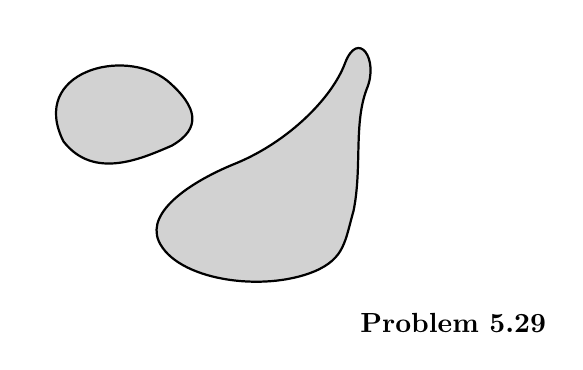
\begin{tikzpicture}[scale=1.1]
  % two irregular conductor cross-sections
  \fill[gray!35] (-1.9,0.6) .. controls (-2.3,1.4) and (-1.2,1.7) .. (-0.7,1.3)
    .. controls (-0.35,1.0) and (-0.3,0.75) .. (-0.65,0.55)
    .. controls (-1.0,0.4) and (-1.55,0.15) .. (-1.9,0.6) -- cycle;
  \draw[thick] (-1.9,0.6) .. controls (-2.3,1.4) and (-1.2,1.7) .. (-0.7,1.3)
    .. controls (-0.35,1.0) and (-0.3,0.75) .. (-0.65,0.55)
    .. controls (-1.0,0.4) and (-1.55,0.15) .. (-1.9,0.6) -- cycle;
  \fill[gray!35] (1.0,-0.9) .. controls (0.4,-1.15) and (-0.6,-1.0) .. (-0.8,-0.55)
    .. controls (-0.95,-0.2) and (-0.4,0.15) .. (0.1,0.35)
    .. controls (0.7,0.6) and (1.2,1.1) .. (1.35,1.5)
    .. controls (1.5,1.9) and (1.75,1.55) .. (1.6,1.2)
    .. controls (1.45,0.8) and (1.55,0.3) .. (1.45,-0.2)
    .. controls (1.35,-0.55) and (1.35,-0.75) .. (1.0,-0.9) -- cycle;
  \draw[thick] (1.0,-0.9) .. controls (0.4,-1.15) and (-0.6,-1.0) .. (-0.8,-0.55)
    .. controls (-0.95,-0.2) and (-0.4,0.15) .. (0.1,0.35)
    .. controls (0.7,0.6) and (1.2,1.1) .. (1.35,1.5)
    .. controls (1.5,1.9) and (1.75,1.55) .. (1.6,1.2)
    .. controls (1.45,0.8) and (1.55,0.3) .. (1.45,-0.2)
    .. controls (1.35,-0.55) and (1.35,-0.75) .. (1.0,-0.9) -- cycle;
  \node at (2.6,-1.5) {\textbf{Problem 5.29}};
\end{tikzpicture}
\end{center}

Show that the product of the inductance per unit length $L$ and the capacitance per unit length $C$ is
\[
LC=\mu\epsilon
\]
where $\mu$ and $\epsilon$ are the permeability and the permittivity of the medium surrounding the conductors. (See the discussion about magnetic fields near perfect conductors at the beginning of Section 5.13.)
\solution
Use the perfect-conductor magnetic boundary condition stated in
Section 5.13: no magnetic field in the conductors and no trapped flux.
Let the electrostatic transverse field for voltage difference $V$
be $\mathbf E$, with charges per length $\pm\lambda$, so $\lambda=C'V$.
In the homogeneous exterior medium, $\mathbf E$ is both curl-free
and divergence-free, and normal to each conductor.

The rotated field
$\mathbf H=\gamma\widehat{\mathbf z}\times\mathbf E$ is consequently
curl-free and divergence-free in the transverse exterior region,
and tangent to the conductor surfaces. On a contour around one wire,
\[
\oint\mathbf H\cdot d\mathbf l
=\gamma\oint\mathbf E\cdot\mathbf n\,dl
=\gamma\frac{\lambda}{\epsilon}=I.
\]
Thus $\gamma=\epsilon I/\lambda$.
The energy relation
$\frac{\epsilon}{2}\int E^2d^2x=C'V^2/2$ then gives
\[
W'_m=\frac{\mu}{2}\int H^2d^2x
=\frac{\mu}{\epsilon}\left(\frac{\epsilon I}{C'V}\right)^2
\frac{C'V^2}{2}
=\frac{\mu\epsilon I^2}{2C'}.
\]
Comparing with $W'_m=L'I^2/2$ proves
$\boxed{L'C'=\mu\epsilon}$.
This result concerns the external inductance of perfect conductors.
An internal magnetic field, such as that of a uniform-current wire
in 5.26, adds internal inductance and does not satisfy this same product.


\Needspace{5\baselineskip}
\par\bigskip
\noindent\textbf{5.30}\quad\begin{enumerate}
\item[(a)] Show that a surface current density $K(\phi)=I\cos\phi/2R$ flowing in the axial direction on a right circular cylindrical surface of radius $R$ produces inside the cylinder a uniform magnetic induction $B_{0}=\mu_{0}I/4R$ in a direction perpendicular to the cylinder axis. Show that the field outside is that of a two-dimensional dipole.
\item[(b)] Calculate the total magnetostatic field energy per unit length. How is it divided inside and outside the cylinder?
\item[(c)] What is the inductance per unit length of the system, viewed as a long circuit with current flowing up one side of the cylinder and back the other?
\end{enumerate}
\textbf{Answer:} $L=\pi\mu_{0}/8$.
\solution
\textbf{(a)} Set $K_z=K_0\cos\phi$, $K_0=I/(2R)$.
The axial vector potential solves the two-dimensional Laplace
equation on either side of the sheet. Regularity, decay of the field,
and continuity give
\[
A_z=C\cos\phi\begin{cases}\rho,&\rho<R,\\R^2/\rho,&\rho>R.\end{cases}
\]
Since $B_\rho=\rho^{-1}\partial_\phi A_z$ and
$B_\phi=-\partial_\rho A_z$,
\[
\mathbf B_{\rm in}=-C\widehat{\mathbf y},\qquad
(B_\rho,B_\phi)_{\rm out}
=\frac{CR^2}{\rho^2}(-\sin\phi,\cos\phi).
\]
The jump $B_{\phi,\rm out}-B_{\phi,\rm in}=\mu_0K_z$ gives
$2C\cos\phi=\mu_0I\cos\phi/(2R)$.
Therefore $\boxed{C=B_0=\mu_0I/(4R)}$, and the exterior field is the
two-dimensional dipole field displayed above.

\textbf{(b)} The energy per length inside is
$W'_{\rm in}=\pi R^2B_0^2/(2\mu_0)$.
Outside the magnitude is $B_0R^2/\rho^2$, so
\[
W'_{\rm out}=\frac1{2\mu_0}\int_R^\infty
\frac{B_0^2R^4}{\rho^4}2\pi\rho\,d\rho
=\frac{\pi R^2B_0^2}{2\mu_0}=W'_{\rm in}.
\]
Thus $\boxed{W'_{\rm total}=\pi\mu_0I^2/16}$, divided equally.

\textbf{(c)} The positive axial current integrates to
$\int_{-\pi/2}^{\pi/2}K_zR\,d\phi=I$; the other half carries $-I$.
Accordingly the circuit current is precisely the $I$ in the density,
and
$\boxed{L'=2W'_{\rm total}/I^2=\pi\mu_0/8}$.


\Needspace{5\baselineskip}
\par\bigskip
\noindent\textbf{5.31}\quad An accelerator bending magnet consists of $N$ turns of superconducting cable whose current configuration can be described approximately by the axial current density
\[
J_{z}(\rho,\phi)=\left(\frac{NI}{2R}\right)\!\cos\phi\;\delta(\rho-R)
\]
The right circular current cylinder is centered on the axis of a hollow iron cylinder of inner radius $R'$ ($R'>R$). The relative dimensions ($R$, $R'$ a few centimeters and a magnet length of several meters) permit the use of a two-dimensional approximation, at least away from the ends of the magnet. Assume that the relative permeability of the iron can be taken as infinite. [Then the outer radius of the iron is irrelevant.]
\begin{enumerate}
\item[(a)] Show that the magnetic field inside the current sheath is perpendicular to the axis of the cylinder in the direction defined by $\phi=\pm\pi/2$ and has the magnitude
\[
B_{0}=\left(\frac{\mu_{0}NI}{4R}\right)\!\left[1+\frac{R^{2}}{R'^{2}}\right]
\]
\item[(b)] Show that the magnetic energy inside $r=R$ is augmented (and that outside diminished) relative to the values in the absence of the iron. (Compare part b of Problem 5.30.)
\item[(c)] Show that the inductance per unit length is
\[
\frac{dL}{dz}=\left(\frac{\pi\mu_{0}N^{2}}{8}\right)\!\left[1+\frac{R^{2}}{R'^{2}}\right]
\]
\end{enumerate}
\solution
Let $c_0=\mu_0NI/(4R)$ and $\eta=R^2/R'^2$.
Write
\[
A_z=\cos\phi\begin{cases}C\rho,&\rho<R,\\
D\rho+E/\rho,&R<\rho<R'.\end{cases}
\]
At the inner face of infinitely permeable iron, tangential $H_\phi$
vanishes, so $D-E/R'^2=0$.
At the current sheath, continuity gives $C=D+E/R^2$ and the derivative
jump gives $2E/R^2=\mu_0NI/(2R)$.
These equations yield
$E=c_0R^2$, $D=c_0\eta$, and $C=c_0(1+\eta)$.

\textbf{(a)} As in 5.30 the core field is along $-y$ for the displayed
positive-current convention and has magnitude
\[
\boxed{B_0=c_0(1+\eta)
=\frac{\mu_0NI}{4R}\left(1+\frac{R^2}{R'^2}\right).}
\]
Reversing the current reverses its direction.

\textbf{(b)} Put $W'_0=\pi R^2c_0^2/(2\mu_0)$, the energy in each
region for the corresponding free-space sheath.
Inside, $W'_{\rm in}=W'_0(1+\eta)^2$.
In the gap,
$B^2=D^2+E^2/\rho^4-2DE\cos(2\phi)/\rho^2$.
Angular integration removes the last term, giving
\[
\begin{split}
W'_{\rm out}
&=\frac{\pi}{\mu_0}\int_R^{R'}
(D^2\rho+E^2/\rho^3)d\rho\\
&=\frac{\pi}{2\mu_0}
[D^2(R'^2-R^2)+E^2(R^{-2}-R'^{-2})]
=\boxed{W'_0(1-\eta^2)}.
\end{split}
\]
The iron contributes zero energy in the infinite-permeability limit.
Thus the interior energy increases and the exterior energy decreases.

\textbf{(c)} Their sum is $2W'_0(1+\eta)$.
Dividing twice this energy by the turn current squared gives
\[
\boxed{L'=\frac{\pi\mu_0N^2}{8}(1+\eta).}
\]
The factor is $N^2$, because $I$ is the current in each turn whereas
the sheet strength is proportional to $NI$.


\Needspace{5\baselineskip}
\par\bigskip
\noindent\textbf{5.32}\quad A circular loop of mean radius $a$ is made of wire having a circular cross section of radius $b$, with $b\ll a$. The sketch shows the relevant dimensions and coordinates for this problem.

\begin{center}
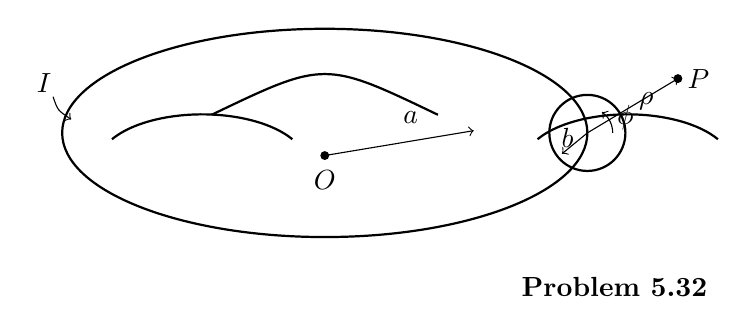
\begin{tikzpicture}[scale=1.15]
  % torus seen obliquely
  \draw[thick] (0,0.35) ellipse (2.9 and 1.15);
  \draw[thick] (-2.35,0.28) arc (150:30:1.15 and 0.55);
  \draw[thick] (2.35,0.28) arc (30:150:-1.15 and 0.55);
  % inner far edge of tube opening
  \draw[thick] (-1.25,0.55) .. controls (0,1.15) and (0,1.15) .. (1.25,0.55);
  % center O
  \fill (0,0.1) circle (1.4pt) node[below=2pt] {$O$};
  % radius a arrow to tube center on right
  \draw[->] (0,0.1) -- (30:1.9 and 0.75);
  \node at (0.95,0.52) {$a$};
  % wire cross-section circle on right
  \draw[thick] (2.9,0.35) circle (0.42);
  % radius b inside the cross-section
  \draw[->] (2.9,0.35) -- (2.62,0.12);
  \node at (2.68,0.3) {$b$};
  % phi angle on the cross-section
  \draw[->] (3.18,0.35) arc (0:55:0.28);
  \node at (3.32,0.52) {$\phi$};
  % rho and P outside
  \draw[->] (2.9,0.35) -- (3.9,0.95);
  \node at (3.55,0.7) {$\rho$};
  \fill (3.9,0.95) circle (1.4pt) node[right] {$P$};
  % current label I on left
  \node at (-3.1,0.9) {$I$};
  \draw[->] (-3.0,0.75) .. controls (-2.95,0.6) .. (-2.8,0.5);
  \node at (3.2,-1.35) {\textbf{Problem 5.32}};
\end{tikzpicture}
\end{center}

\begin{enumerate}
\item[(a)] Using (5.37), the expression for the vector potential of a filamentary circular loop, and appropriate approximations for the elliptic integrals, show that the vector potential at the point $P$ near the wire is approximately
\[
A_{\phi}=(\mu_{0}I/2\pi)[\ln(8a/\rho)-2]
\]
where $\rho$ is the transverse coordinate shown in the figure and corrections are of order $(\rho/a)\cos\phi$ and $(\rho/a)^{2}$.
\item[(b)] Since the vector potential of part a is, apart from a constant, just that outside a straight circular wire carrying a current $I$, determine the vector potential inside the wire ($\rho<b$) in the same approximation by requiring continuity of $A_{\phi}$ and its radial derivative at $\rho=b$, assuming that the current is uniform in density inside the wire:
\[
A_{\phi}=(\mu_{0}I/4\pi)(1-\rho^{2}/b^{2})+(\mu_{0}I/2\pi)[\ln(8a/b)-2],\qquad\rho<b
\]
\item[(c)] Use (5.149) to find the magnetic energy, hence the self-inductance,
\[
L=\mu_{0}a[\ln(8a/b)-7/4]
\]
Are the corrections of order $b/a$ or $(b/a)^{2}$? What is the change in $L$ if the current is assumed to flow only on the surface of the wire (as occurs at high frequencies when the skin depth is small compared to $b$)?
\end{enumerate}
\solution
Distinguish the large cylindrical radius $s$ about the loop axis
from the small local distance $\rho$ from the wire center.
Near the wire, $s=a+\rho\cos\phi$ and $z=\rho\sin\phi$.

\textbf{(a)} From the circular-loop potential, or 5.28 divided by the
circumference $2\pi s$,
\[
A_\varphi=\frac{\mu_0I}{\pi k}\sqrt{\frac as}
\left[\left(1-\frac{k^2}{2}\right)K(k)-E(k)\right],
\quad
k^2=\frac{4as}{(a+s)^2+z^2}.
\]
The complementary modulus is
$k'=\rho/\sqrt{(a+s)^2+z^2}=\rho/(2a)[1+O(\rho/a)]$.
Use $K=\ln(4/k')+O(k'^2\ln k')$ and
$E=1+O(k'^2\ln k')$, with $s\simeq a$, $k\simeq1$:
\[
\boxed{A_\varphi\simeq\frac{\mu_0I}{2\pi}
\left[\ln\frac{8a}{\rho}-2\right].}
\]
The first geometrical correction is proportional to
$(\rho/a)\cos\phi$ (with logarithmic coefficients), followed by
second-order terms. The local angle $\phi$ in the figure is not the
azimuth $\varphi$ specifying the direction of this vector potential.

\textbf{(b)} Locally the straight-wire equation is
$\rho^{-1}(\rho A_\varphi')'=-\mu_0I/(\pi b^2)$.
Integrate once and discard the singular $1/\rho$ derivative at the center:
$A_\varphi'=-\mu_0I\rho/(2\pi b^2)$.
Matching its value to the exterior potential at $\rho=b$ gives
\[
\boxed{A_\varphi=\frac{\mu_0I}{4\pi}\left(1-\frac{\rho^2}{b^2}\right)
+\frac{\mu_0I}{2\pi}\left[\ln\frac{8a}{b}-2\right],\quad\rho<b.}
\]
Its derivative at $b$ is $-\mu_0I/(2\pi b)$, also matching outside.

\textbf{(c)} To this order the volume element is
$2\pi a\,d^2\rho$, and $J=I/(\pi b^2)$.
Since $\langle\rho^2\rangle=b^2/2$ in a uniform disk,
\[
\langle A_\varphi\rangle
=\frac{\mu_0I}{8\pi}
+\frac{\mu_0I}{2\pi}\left[\ln\frac{8a}{b}-2\right]
=\frac{\mu_0I}{2\pi}\left[\ln\frac{8a}{b}-\frac74\right].
\]
Therefore
$W=\tfrac12(2\pi a)I\langle A_\varphi\rangle$
and
\[
\boxed{L=\mu_0a\left[\ln\frac{8a}{b}-\frac74\right].}
\]
Every first-order curvature term contains $\cos\phi$ and averages
to zero, including the first correction to the toroidal volume
element. The surviving corrections start at second order in $b/a$,
possibly multiplied by $\ln(a/b)$.
For surface current the local internal field and its internal energy
vanish; use $A_\varphi(b)$ in the energy integral instead. Then
\[
\boxed{L_{\rm surface}=\mu_0a\left[\ln\frac{8a}{b}-2\right]
=L-\frac{\mu_0a}{4}.}
\]


\Needspace{5\baselineskip}
\par\bigskip
\noindent\textbf{5.33}\quad Consider two current loops (as in Fig.~5.3) whose orientation in space is fixed, but whose relative separation can be changed. Let $O_{1}$ and $O_{2}$ be origins in the two loops, fixed relative to each loop, and $\mathbf{x}_{1}$ and $\mathbf{x}_{2}$ be coordinates of elements $d\mathbf{l}_{1}$ and $d\mathbf{l}_{2}$, respectively, of the loops referred to the respective origins. Let $\mathbf{R}$ be the relative coordinate of the origins, directed from loop 2 to loop 1.
\begin{enumerate}
\item[(a)] Starting from (5.10), the expression for the force between the loops, show that it can be written
\[
\mathbf{F}_{12}=I_{1}I_{2}\nabla_{R}M_{12}(\mathbf{R})
\]
where $M_{12}$ is the mutual inductance of the loops,
\[
M_{12}(\mathbf{R})=\frac{\mu_{0}}{4\pi}\oint\oint\frac{d\mathbf{l}_{1}\cdot d\mathbf{l}_{2}}{|\mathbf{x}_{1}-\mathbf{x}_{2}+\mathbf{R}|}
\]
and it is assumed that the orientation of the loops does not change with $\mathbf{R}$.
\item[(b)] Show that the mutual inductance, viewed as a function of $\mathbf{R}$ \erratum{in any open region where the two filaments do not intersect}, is a solution of the Laplace equation,
\[
\nabla_{R}^{2}M_{12}(\mathbf{R})=0
\]
The importance of this result is that the uniqueness of solutions of the Laplace equation allows the exploitation of the properties of such solutions, provided a solution can be found for a particular value of $\mathbf{R}$.
\end{enumerate}
\solution
\textbf{(a)} Put
$\mathbf s=\mathbf x_1-\mathbf x_2+\mathbf R$.
The magnetic force on loop 1 is
\[
\mathbf F_{12}=\frac{\mu_0I_1I_2}{4\pi}
\oint\oint\frac{d\mathbf l_1\times(d\mathbf l_2\times\mathbf s)}{s^3}.
\]
Expanding the triple product gives
$d\mathbf l_2(d\mathbf l_1\cdot\mathbf s)
-\mathbf s(d\mathbf l_1\cdot d\mathbf l_2)$.
For fixed loop-2 element,
$d\mathbf l_1\cdot\mathbf s/s^3=-d(1/s)$, whose integral around
closed loop 1 is zero. The remaining term is
$(d\mathbf l_1\cdot d\mathbf l_2)\nabla_R(1/s)$.
The loop orientations and their local coordinates are independent
of $\mathbf R$, so the derivative can be taken outside:
\[
\boxed{\mathbf F_{12}=I_1I_2\nabla_RM_{12},\qquad
M_{12}=\frac{\mu_0}{4\pi}\oint\oint
\frac{d\mathbf l_1\cdot d\mathbf l_2}{|\mathbf x_1-\mathbf x_2+\mathbf R|}.}
\]
\textbf{(b)} For any open set of separations in which the filaments
are disjoint, $s>0$ and $\nabla_R^2(1/s)=0$ throughout the integration.
Consequently $\boxed{\nabla_R^2M_{12}=0}$ in that set.
This qualification matters: at intersecting-loop separations, the
distributional identity instead reads
\[
\nabla_R^2M_{12}=-\mu_0\oint\oint d\mathbf l_1\cdot d\mathbf l_2\,
\delta^3(\mathbf R+\mathbf x_1-\mathbf x_2).
\]
Uniqueness and harmonic continuation are therefore used only within
a current-free region of separation space.


\Needspace{5\baselineskip}
\par\bigskip
\noindent\textbf{5.34}\quad Two identical circular loops of radius $a$ are initially located a distance $R$ apart on a common axis perpendicular to their planes.
\begin{enumerate}
\item[(a)] From the expression $W_{12}=\int d^{3}x\,\mathbf{J}_{1}\cdot\mathbf{A}_{2}$ and the result for $A_{\phi}$ from Problem 5.10b, show that the mutual inductance of the loops is
\[
M_{12}=\mu_{0}\pi a^{2}\int_{0}^{\infty}dk\;e^{-kR}J_{1}^{2}(ka)
\]
\item[(b)] Show that for $R>2a$, $M_{12}$ has the expansion,
\[
M_{12}=\frac{\mu_{0}\pi a}{2}\left[\left(\frac{a}{R}\right)^{3}-3\left(\frac{a}{R}\right)^{5}+\frac{75}{8}\left(\frac{a}{R}\right)^{7}+\cdots\right]
\]
\item[(c)] Use the techniques of Section 3.3 for solutions of the Laplace equation to show that the mutual inductance for two coplanar identical circular loops of radius $a$ whose centers are separated by a distance $R>2a$ is
\[
M_{12}=-\frac{\mu_{0}\pi a}{4}\left[\left(\frac{a}{R}\right)^{3}+\frac{9}{4}\left(\frac{a}{R}\right)^{5}+\frac{375}{64}\left(\frac{a}{R}\right)^{7}+\cdots\right]
\]
\item[(d)] Calculate the forces between the loops in the common axis and coplanar configurations. Relate the answers to those of Problem 5.18.
\end{enumerate}
\solution
\textbf{(a)} The azimuthal potential of loop 1 on loop 2 is constant.
Multiplying the result in 5.10(b) at $\rho=a,z=R$ by $2\pi aI_2$ gives
$W_{12}=I_1I_2M_{12}$ with
\[
\boxed{M_\parallel(R)=\mu_0\pi a^2
\int_0^\infty e^{-kR}J_1(ka)^2\,dk.}
\]
\textbf{(b)} The power series
$J_1(x)=\sum_{j\ge0}(-1)^j(x/2)^{2j+1}/[j!(j+1)!]$
gives
\[
J_1(x)^2=\frac{x^2}{4}-\frac{x^4}{16}
+\frac{5x^6}{768}+\cdots.
\]
More generally its coefficient of $(-1)^n(x/2)^{2n+2}$ is
\[
\sum_{j=0}^n\frac1{j!(j+1)!(n-j)!(n-j+1)!}
=\frac{(2n+2)!}{n!(n+2)![(n+1)!]^2}.
\]
This follows by factoring out $1/[n!(n+2)!]$ and applying the
binomial convolution to $\sum_j\binom nj\binom{n+2}{j+1}$.
Integrating each term with
$\int_0^\infty k^m e^{-kR}dk=m!/R^{m+1}$ gives
\[
M_\parallel(R)=\mu_0\pi a\sum_{n=0}^\infty
(-1)^nD_n(a/R)^{2n+3},
\quad
D_n=\frac{[(2n+2)!]^2}{2^{2n+2}n!(n+2)![(n+1)!]^2}.
\]
The ratio test gives convergence for $R>2a$.
For $n=0,1,2$, $D_n=1/2,3/2,75/16$, yielding
\[
\boxed{M_\parallel=\frac{\mu_0\pi a}{2}
\left[(a/R)^3-3(a/R)^5+\frac{75}{8}(a/R)^7+\cdots\right].}
\]
\textbf{(c)} With parallel loop normals fixed, rotational symmetry
makes $M(\mathbf R)$ axisymmetric in separation space.
By 5.33 it is harmonic for $R>2a$ and decays at infinity.
The exterior harmonic with axial value $R^{-2n-3}$ is
$R^{-2n-3}P_{2n+2}(\cos\Theta)$.
Thus replace each term by this angular form.
At $\Theta=\pi/2$,
\[
P_{2n+2}(0)=(-1)^{n+1}
\frac{(2n+2)!}{2^{2n+2}[(n+1)!]^2},
\]
so all terms in the coplanar mutual inductance are negative:
\[
\boxed{M_\perp=-\frac{\mu_0\pi a}{4}
\left[(a/R)^3+\frac94(a/R)^5+\frac{375}{64}(a/R)^7+\cdots\right].}
\]
\textbf{(d)} At fixed currents, $F_R=I_1I_2\,dM/dR$.
For positive $I_1I_2$,
\[
\boxed{F_{R,\parallel}=-\frac{3\mu_0\pi I_1I_2}{2}
(a/R)^4\left[1-5(a/R)^2+\frac{175}{8}(a/R)^4+\cdots\right],}
\]
\[
\boxed{F_{R,\perp}=+\frac{3\mu_0\pi I_1I_2}{4}
(a/R)^4\left[1+\frac{15}{4}(a/R)^2+\frac{875}{64}(a/R)^4+\cdots\right].}
\]
Coaxial like-current loops attract; coplanar like-current loops repel.
Reverse one current and both forces reverse.
For 5.18 use $R=2d$ and $I_2=\chi I_1$ in the axial case,
but $I_2=-\chi I_1$ in the coplanar case. Both then attract a
more-permeable slab, with precisely the two dipole limits found there.


\Needspace{5\baselineskip}
\par\bigskip
\noindent\textbf{5.35}\quad An insulated coil is wound on the surface of a sphere of radius $a$ in such a way as to produce a uniform magnetic induction $B_{0}$ in the $z$ direction inside the sphere and dipole field outside the sphere. The medium inside and outside the sphere has a uniform conductivity $\sigma$ and permeability $\mu$.
\begin{enumerate}
\item[(a)] Find the necessary surface current density $\mathbf{K}$ and show that the vector potential describing the magnetic field has only an azimuthal component, given by
\[
A_{\phi}=\frac{B_{0}a^{2}}{2}\frac{r_{<}}{r_{>}^{2}}\sin\theta
\]
where $r_{<}$ ($r_{>}$) is the smaller (larger) of $r$ and $a$.
\item[(b)] At $t=0$ the current in the coil is cut off. [The coil's presence may be ignored from now on.] With the neglect of Maxwell's displacement current, the decay of the magnetic field is described by the diffusion equation, (5.160). Using a Laplace transform and a spherical Bessel function expansion (3.113), show that the vector potential at times $t>0$ is given by
\[
A_{\phi}=\frac{3B_{0}a}{\pi}\sin\theta\int_{0}^{\infty}e^{-\nu tk^{2}}j_{1}(k)j_{1}\!\left(\frac{kr}{a}\right)dk
\]
where $\nu=1/\mu\sigma a^{2}$ is a characteristic decay rate and $j_{1}(x)$ is the spherical Bessel function of order one. Show that the magnetic field at the center of the sphere can be written explicitly in terms of the error function $\Phi(x)$ as
\[
B_{z}(0,t)=B_{0}\!\left[\Phi\!\left(\frac{1}{\sqrt{4\nu t}}\right)-\frac{1}{\sqrt{\pi\nu t}}\exp\!\left(-\frac{1}{4\nu t}\right)\right]
\]
\item[(c)] Show that the total magnetic energy at time $t>0$ can be written
\[
W_{\mathrm{m}}=\frac{6B_{0}^{2}a^{3}}{\mu}\int_{0}^{\infty}e^{-2\nu tk^{2}}[j_{1}(k)]^{2}\;dk
\]
Show that at long times ($\nu t\gg1$) the magnetic energy decays asymptotically as
\[
W_{\mathrm{m}}\to\frac{\sqrt{2\pi}B_{0}^{2}a^{3}}{24\mu(\nu t)^{3/2}}
\]
\item[(d)] Find a corresponding expression for the asymptotic form of the vector potential (at fixed $r$, $\theta$ and $\nu t\to\infty$) and show that it decays as $(\nu t)^{-3/2}$ as well. Since the energy is quadratic in the field strength, there seems to be a puzzle here. Show by numerical or analytic means that the behavior of the magnetic field at time $t$ is such that, for distances small compared to $R=a(\nu t)^{1/2}\gg a$, the field is uniform with strength $(B_{0}/6\pi^{1/2})\,(\nu t)^{-3/2}$, and for distances large compared to $R$, the field is essentially the original dipole field. Explain physically.
\end{enumerate}
\solution
\textbf{(a)} Write $A_\phi=f(r)\sin\theta$.
A uniform interior field requires $f=B_0r/2$.
Continuity with the decaying exterior dipole requires
$f=B_0a^3/(2r^2)$ outside. Thus
\[
\boxed{A_\phi=\frac{B_0a^2}{2}\frac{r_<}{r_>^2}\sin\theta.}
\]
Its curl gives $B_{r,\rm in}=B_0\cos\theta$,
$B_{\theta,\rm in}=-B_0\sin\theta$, and
$B_{r,\rm out}=B_0(a/r)^3\cos\theta$,
$B_{\theta,\rm out}=(B_0/2)(a/r)^3\sin\theta$.
The tangential jump is $3B_0\sin\theta/2$, so
\[
\boxed{\mathbf K=\frac{3B_0}{2\mu}\sin\theta\,\widehat{\boldsymbol\phi}.}
\]
\textbf{(b)} Put $x=r/a$, $\tau=\nu t$, $\nu=(\mu\sigma a^2)^{-1}$.
The vector diffusion equation reduces to
\[
\partial_tf=\nu\mathcal L_xf,\qquad
\mathcal L_x=\frac{d^2}{dx^2}+\frac2x\frac d{dx}-\frac2{x^2}.
\]
Initially $f=(B_0a/2)g(x)$ with $g=x$ for $x<1$ and $g=x^{-2}$
for $x>1$. Since $g$ is continuous and its first derivative jumps
from $1$ to $-2$, $\mathcal L_xg=-3\delta(x-1)$.
The spherical Bessel functions satisfy
$\mathcal L_xj_1(kx)=-k^2j_1(kx)$ and
\[
\int_0^\infty x^2j_1(kx)j_1(qx)dx
=\frac{\pi}{2k^2}\delta(k-q).
\]
The radial operator is self-adjoint with weight $x^2$: integrating
$u\mathcal L_xv-v\mathcal L_xu$ gives
$[x^2(uv'-u'v)]_0^\infty$. Apply this to $u=j_1(kx)$ and $v=g(x)$,
with a vanishing positive convergence factor at infinity if needed for
the oscillatory integral. The endpoint term vanishes, leaving the
derivative jump at $x=1$. Hence the initial transform satisfies
\[
-k^2\int_0^\infty x^2g(x)j_1(kx)dx
=\int_0^\infty x^2j_1(kx)\mathcal L_xg(x)dx=-3j_1(k).
\]
Thus $\widetilde g(k)=3j_1(k)/k^2$.
Laplace transformation in time gives
$(p+\nu k^2)\overline{\widetilde f}(k,p)
=(B_0a/2)\widetilde g(k)$.
Inverting the Laplace transform yields $e^{-\nu k^2t}$;
inverting the spherical Bessel transform, with measure $2k^2dk/\pi$,
then gives
\[
\boxed{A_\phi=\frac{3B_0a}{\pi}\sin\theta
\int_0^\infty e^{-\tau k^2}j_1(k)j_1(kx)dk.}
\]
Near the center $j_1(kx)=kx/3+O(x^3)$ and a potential
$A_\phi=Cr\sin\theta$ has $B_z=2C$. Hence
\[
B_z(0,t)=\frac{2B_0}{\pi}\int_0^\infty e^{-\tau k^2}
\left(\frac{\sin k}{k}-\cos k\right)dk.
\]
The cosine Gaussian integral is
$\sqrt\pi\,e^{-u^2/(4\tau)}/(2\sqrt\tau)$.
Integrating this identity from $u=0$ to $u=1$ gives
$\int e^{-\tau k^2}\sin k\,dk/k=(\pi/2)\operatorname{erf}(1/(2\sqrt\tau))$.
Therefore
\[
\boxed{B_z(0,t)=B_0\left[
\operatorname{erf}\frac1{2\sqrt\tau}
-\frac{e^{-1/(4\tau)}}{\sqrt{\pi\tau}}\right].}
\]
The question's $\Phi$ denotes this error function, not an electrostatic
potential. The expression tends to $B_0$ as $t\downarrow0$.

\textbf{(c)} Integration by parts gives
$\int B^2d^3x=\int\mathbf A\cdot(-\nabla^2\mathbf A)d^3x$.
The angular integral is $\int\sin^2\theta\,d\Omega=8\pi/3$, so
\[
W_m=\frac{4\pi}{3\mu}\int_0^\infty r^2f(-\mathcal L_rf)\,dr.
\]
Insert the two Bessel integrals for $f$ and $-\mathcal L_rf$.
The second supplies $k^2/a^2$; orthogonality in physical radius gives
$\pi a^3\delta(k-q)/(2k^2)$.
The prefactors reduce to
$(4\pi/3\mu)(3B_0a/\pi)^2(\pi a/2)=6B_0^2a^3/\mu$:
\[
\boxed{W_m=\frac{6B_0^2a^3}{\mu}
\int_0^\infty e^{-2\tau k^2}j_1(k)^2dk.}
\]
At $\tau\gg1$, only $k=O(\tau^{-1/2})$ contributes.
Use $j_1(k)=k/3+O(k^3)$ and
$\int_0^\infty k^2e^{-2\tau k^2}dk=\sqrt\pi/[4(2\tau)^{3/2}]$:
\[
\boxed{W_m\sim\frac{\sqrt{2\pi}B_0^2a^3}{24\mu\,\tau^{3/2}}.}
\]
As a normalization check, the initial energy is the sum of the uniform
interior contribution $2\pi B_0^2a^3/(3\mu)$ and the exterior dipole
contribution $\pi B_0^2a^3/(3\mu)$, namely $\pi B_0^2a^3/\mu$.
The integral formula agrees, since $\int_0^\infty j_1(k)^2dk=\pi/6$.

\textbf{(d)} At fixed $r$, expand both Bessel factors:
\[
A_\phi\sim\frac{3B_0a}{\pi}\frac{x}{9}\sin\theta
\int_0^\infty k^2e^{-\tau k^2}dk
=\boxed{\frac{B_0r\sin\theta}{12\sqrt\pi}\tau^{-3/2}.}
\]
To describe the changing spatial scale, keep $x/\sqrt\tau$ finite
and expand only $j_1(k)$. The remaining integral can be evaluated:
\[
A_\phi\sim\frac{B_0a^3}{2r^2}\mathcal F(s)\sin\theta,\qquad
s=\frac{r}{2a\sqrt\tau},\quad
\mathcal F(s)=\operatorname{erf}s-\frac{2s}{\sqrt\pi}e^{-s^2}.
\]
Indeed the integral of $ke^{-\tau k^2}j_1(kx)$ is
$\pi\mathcal F(x/(2\sqrt\tau))/(2x^2)$, by the same sine and cosine
integrals used for the center field.
Taking the curl gives
\[
B_r\sim\frac{B_0a^3}{r^3}\mathcal F(s)\cos\theta,\qquad
B_\theta\sim\frac{B_0a^3}{2r^3}
[\mathcal F(s)-s\mathcal F'(s)]\sin\theta.
\]
For $s\ll1$, $\mathcal F(s)=4s^3/(3\sqrt\pi)+O(s^5)$, so the
field is uniform to leading order, with
$\boxed{B_{\rm core}\sim B_0\tau^{-3/2}/(6\sqrt\pi)}$.
For $s\gg1$, $\mathcal F\to1$ and $\mathcal F'\to0$, giving the
original dipole field.

There is no conflict between field and total-energy decay: the nearly
uniform region grows to radius $R=O(a\sqrt\tau)$.
Its energy scales as $B_{\rm core}^2R^3\sim\tau^{-3}\tau^{3/2}$.
The exterior dipole energy beyond $R$ scales as $R^{-3}$, the same
$\tau^{-3/2}$. Magnetic diffusion changes a progressively larger
volume; it does not multiply a fixed spatial field shape by one
time-dependent amplitude.


\Needspace{5\baselineskip}
\par\bigskip
\noindent\textbf{5.36}\quad The time-varying magnetic field for $t>0$ in Problem 5.35 induces an electric field and causes current to flow.
\begin{enumerate}
\item[(a)] What components of electric field exist? Determine integral expressions for the components of the electric field and find a simple explicit form of the current density $\mathbf{J}=\sigma\mathbf{E}$ at $t=0^{+}$. Compare your result with the current density of Problem 5.35a. Find the asymptotic behavior of the electric fields in time.
\item[(b)] With Ohm's law and the electric fields found in part a, show that the total power dissipated in the resistive medium can be written
\[
P=\frac{12B_{0}^{2}a^{3}\nu}{\mu}\int_{0}^{\infty}e^{-2\nu tk^{2}}[kj_{1}(k)]^{2}\;dk
\]
Note that the power is the negative time derivative of the \emph{magnetic} energy, $W_{\mathrm{m}}$.
\item[(c)] Because of Ohm's law, the total \emph{electric} energy is $W_{\mathrm{e}}=\epsilon_{0}P/2\sigma$. The total energy is the sum of $W_{\mathrm{e}}$ and $W_{\mathrm{m}}$; its time derivative should be the negative of the power dissipation. Show that the neglect of the energy in the electric field is the same order of approximation as neglect of the displacement current in the equations governing the magnetic field.
\end{enumerate}
\solution
\textbf{(a)} There are no imposed electric charges or scalar-potential
gradients in this axially symmetric diffusion problem. In the
divergence-free gauge,
$\mathbf E=-\partial_t\mathbf A$, so $E_r=E_\theta=0$ and
\[
\boxed{E_\phi(r,\theta,t)=\frac{3B_0a\nu}{\pi}\sin\theta
\int_0^\infty k^2e^{-\tau k^2}j_1(k)j_1(kr/a)dk.}
\]
At $t=0^+$ use $\partial_tf=\nu\mathcal L_xf$ and the initial
$\mathcal L_xg=-3\delta(x-1)$ found in 5.35:
\[
E_\phi(0^+)=\frac{3B_0a\nu}{2}\sin\theta\,\delta(r/a-1)
=\frac{3B_0a^2\nu}{2}\sin\theta\,\delta(r-a).
\]
Since $\sigma a^2\nu=1/\mu$,
\[
\boxed{\mathbf J(0^+)=\frac{3B_0}{2\mu}
\sin\theta\,\delta(r-a)\widehat{\boldsymbol\phi}.}
\]
This induced sheet current initially replaces exactly the switched-off
coil current in 5.35(a). It is a distributional limit: at every positive
time diffusion smooths the sheet, and the instantaneous switch has a
singular initial dissipation in the ideal diffusion model.
For fixed $r$ at late times, differentiate the asymptotic potential:
\[
\boxed{E_\phi\sim\frac{B_0\nu r\sin\theta}{8\sqrt\pi}\tau^{-5/2}.}
\]
This limit is not uniform over radii of order $a\sqrt\tau$ or larger.

\textbf{(b)} Ohmic dissipation is $P=\sigma\int E_\phi^2d^3x$.
The angular integral is again $8\pi/3$, and the physical radial
orthogonality integral is $\pi a^3\delta(k-q)/(2k^2)$.
Consequently
\[
P=\sigma\left(\frac{3B_0a\nu}{\pi}\right)^2
\frac{8\pi}{3}\frac{\pi a^3}{2}
\int_0^\infty k^2e^{-2\tau k^2}j_1(k)^2dk.
\]
Using $\sigma a^2\nu=1/\mu$ reduces this to
\[
\boxed{P=\frac{12B_0^2a^3\nu}{\mu}
\int_0^\infty e^{-2\tau k^2}[kj_1(k)]^2dk
=-\frac{dW_m}{dt}.}
\]
The equality follows independently by differentiating the energy
integral in 5.35(c) for $t>0$.

\textbf{(c)} Because $\mathbf J=\sigma\mathbf E$,
$P=\sigma\int E^2d^3x$, whereas
$W_e=(\epsilon_0/2)\int E^2d^3x$.
Thus $W_e=\epsilon_0P/(2\sigma)$ as stated.
If the fields vary on a time scale $T$, the displacement-to-conduction
current ratio is
\[
\frac{|\epsilon_0\partial_t\mathbf E|}{|\sigma\mathbf E|}
=O\left(\frac{\epsilon_0}{\sigma T}\right).
\]
In the energy balance, the discarded term has the same relative order:
\[
\frac{|dW_e/dt|}{P}
=\frac{\epsilon_0}{2\sigma}\left|\frac{d\ln P}{dt}\right|
=O\left(\frac{\epsilon_0}{\sigma T}\right).
\]
For example, at late times $W_m\propto t^{-3/2}$ and
$P=(3/2)W_m/t\propto t^{-5/2}$, so
$W_e/W_m=3\epsilon_0/(4\sigma t)$ and
$|dW_e/dt|/P=5\epsilon_0/(4\sigma t)$.
Thus retaining electric energy while omitting displacement current
would mix approximation orders. For times comparable to
$\epsilon_0/\sigma$, the neglected current and electric energy must
both be restored; the ideal $t=0^+$ sheet limit is not a claim that
the quasistatic model resolves arbitrarily fast switching.
